\documentclass[twoside]{book}

% Packages required by doxygen
\usepackage{fixltx2e}
\usepackage{calc}
\usepackage{doxygen}
\usepackage{graphicx}
\usepackage[utf8]{inputenc}
\usepackage{makeidx}
\usepackage{multicol}
\usepackage{multirow}
\PassOptionsToPackage{warn}{textcomp}
\usepackage{textcomp}
\usepackage[nointegrals]{wasysym}
\usepackage[table]{xcolor}

% Font selection
\usepackage[T1]{fontenc}
\usepackage{mathptmx}
\usepackage[scaled=.90]{helvet}
\usepackage{courier}
\usepackage{amssymb}
\usepackage{sectsty}
\renewcommand{\familydefault}{\sfdefault}
\allsectionsfont{%
  \fontseries{bc}\selectfont%
  \color{darkgray}%
}
\renewcommand{\DoxyLabelFont}{%
  \fontseries{bc}\selectfont%
  \color{darkgray}%
}
\newcommand{\+}{\discretionary{\mbox{\scriptsize$\hookleftarrow$}}{}{}}

% Page & text layout
\usepackage{geometry}
\geometry{%
  a4paper,%
  top=2.5cm,%
  bottom=2.5cm,%
  left=2.5cm,%
  right=2.5cm%
}
\tolerance=750
\hfuzz=15pt
\hbadness=750
\setlength{\emergencystretch}{15pt}
\setlength{\parindent}{0cm}
\setlength{\parskip}{0.2cm}
\makeatletter
\renewcommand{\paragraph}{%
  \@startsection{paragraph}{4}{0ex}{-1.0ex}{1.0ex}{%
    \normalfont\normalsize\bfseries\SS@parafont%
  }%
}
\renewcommand{\subparagraph}{%
  \@startsection{subparagraph}{5}{0ex}{-1.0ex}{1.0ex}{%
    \normalfont\normalsize\bfseries\SS@subparafont%
  }%
}
\makeatother

% Headers & footers
\usepackage{fancyhdr}
\pagestyle{fancyplain}
\fancyhead[LE]{\fancyplain{}{\bfseries\thepage}}
\fancyhead[CE]{\fancyplain{}{}}
\fancyhead[RE]{\fancyplain{}{\bfseries\leftmark}}
\fancyhead[LO]{\fancyplain{}{\bfseries\rightmark}}
\fancyhead[CO]{\fancyplain{}{}}
\fancyhead[RO]{\fancyplain{}{\bfseries\thepage}}
\fancyfoot[LE]{\fancyplain{}{}}
\fancyfoot[CE]{\fancyplain{}{}}
\fancyfoot[RE]{\fancyplain{}{\bfseries\scriptsize Generated on Tue Jun 17 2014 10\+:06\+:55 for P\+F\+Q-\/\+Lang e\+D\+L\+S by Doxygen }}
\fancyfoot[LO]{\fancyplain{}{\bfseries\scriptsize Generated on Tue Jun 17 2014 10\+:06\+:55 for P\+F\+Q-\/\+Lang e\+D\+L\+S by Doxygen }}
\fancyfoot[CO]{\fancyplain{}{}}
\fancyfoot[RO]{\fancyplain{}{}}
\renewcommand{\footrulewidth}{0.4pt}
\renewcommand{\chaptermark}[1]{%
  \markboth{#1}{}%
}
\renewcommand{\sectionmark}[1]{%
  \markright{\thesection\ #1}%
}

% Indices & bibliography
\usepackage{natbib}
\usepackage[titles]{tocloft}
\setcounter{tocdepth}{3}
\setcounter{secnumdepth}{5}
\makeindex

% Hyperlinks (required, but should be loaded last)
\usepackage{ifpdf}
\ifpdf
  \usepackage[pdftex,pagebackref=true]{hyperref}
\else
  \usepackage[ps2pdf,pagebackref=true]{hyperref}
\fi
\hypersetup{%
  colorlinks=true,%
  linkcolor=blue,%
  citecolor=blue,%
  unicode%
}

% Custom commands
\newcommand{\clearemptydoublepage}{%
  \newpage{\pagestyle{empty}\cleardoublepage}%
}


%===== C O N T E N T S =====

\begin{document}

% Titlepage & ToC
\hypersetup{pageanchor=false,
             bookmarks=true,
             bookmarksnumbered=true,
             pdfencoding=unicode
            }
\pagenumbering{roman}
\begin{titlepage}
\vspace*{7cm}
\begin{center}%
{\Large P\+F\+Q-\/\+Lang e\+D\+L\+S \\[1ex]\large v3.\+0 }\\
\vspace*{1cm}
{\large Generated by Doxygen 1.8.7}\\
\vspace*{0.5cm}
{\small Tue Jun 17 2014 10:06:55}\\
\end{center}
\end{titlepage}
\clearemptydoublepage
\tableofcontents
\clearemptydoublepage
\pagenumbering{arabic}
\hypersetup{pageanchor=true}

%--- Begin generated contents ---
\chapter{Namespace Index}
\section{Namespace List}
Here is a list of all namespaces with brief descriptions\+:\begin{DoxyCompactList}
\item\contentsline{section}{\hyperlink{namespacepfq__lang}{pfq\+\_\+lang} }{\pageref{namespacepfq__lang}}{}
\item\contentsline{section}{\hyperlink{namespacepfq__lang_1_1anonymous__namespace_02default_8hpp_03}{pfq\+\_\+lang\+::anonymous\+\_\+namespace\{default.\+hpp\}} }{\pageref{namespacepfq__lang_1_1anonymous__namespace_02default_8hpp_03}}{}
\item\contentsline{section}{\hyperlink{namespacepfq__lang_1_1term}{pfq\+\_\+lang\+::term} }{\pageref{namespacepfq__lang_1_1term}}{}
\end{DoxyCompactList}

\chapter{Hierarchical Index}
\section{Class Hierarchy}
This inheritance list is sorted roughly, but not completely, alphabetically\+:\begin{DoxyCompactList}
\item \contentsline{section}{pfq\+:\+:lang\+:\+:Action$<$ a $>$}{\pageref{structpfq_1_1lang_1_1Action}}{}
\item \contentsline{section}{pfq\+:\+:lang\+:\+:Argument}{\pageref{structpfq_1_1lang_1_1Argument}}{}
\item bool\+\_\+type\begin{DoxyCompactList}
\item \contentsline{section}{pfq\+:\+:lang\+:\+:has\+\_\+insertion\+\_\+operator$<$ T $>$}{\pageref{structpfq_1_1lang_1_1has__insertion__operator}}{}
\item \contentsline{section}{pfq\+:\+:lang\+:\+:is\+\_\+mfunction$<$ Tp $>$}{\pageref{structpfq_1_1lang_1_1is__mfunction}}{}
\item \contentsline{section}{pfq\+:\+:lang\+:\+:is\+\_\+predicate$<$ Tp $>$}{\pageref{structpfq_1_1lang_1_1is__predicate}}{}
\item \contentsline{section}{pfq\+:\+:lang\+:\+:is\+\_\+property$<$ Tp $>$}{\pageref{structpfq_1_1lang_1_1is__property}}{}
\end{DoxyCompactList}
\item \contentsline{section}{pfq\+:\+:lang\+:\+:Composition$<$ F, G $>$}{\pageref{structpfq_1_1lang_1_1Composition}}{}
\item false\+\_\+type\begin{DoxyCompactList}
\item \contentsline{section}{pfq\+:\+:lang\+:\+:is\+\_\+\+Function$<$ Tp $>$}{\pageref{structpfq_1_1lang_1_1is__Function}}{}
\item \contentsline{section}{pfq\+:\+:lang\+:\+:is\+\_\+same\+\_\+type\+\_\+constructor$<$ T, Tp $>$}{\pageref{structpfq_1_1lang_1_1is__same__type__constructor}}{}
\end{DoxyCompactList}
\item \contentsline{section}{pfq\+:\+:lang\+:\+:Function$<$ Sig $>$}{\pageref{structpfq_1_1lang_1_1Function}}{}
\begin{DoxyCompactList}
\item \contentsline{section}{pfq\+:\+:lang\+:\+:Combinator1$<$ Pred $>$}{\pageref{structpfq_1_1lang_1_1Combinator1}}{}
\item \contentsline{section}{pfq\+:\+:lang\+:\+:Combinator2$<$ Pred1, Pred2 $>$}{\pageref{structpfq_1_1lang_1_1Combinator2}}{}
\item \contentsline{section}{pfq\+:\+:lang\+:\+:M\+Function}{\pageref{structpfq_1_1lang_1_1MFunction}}{}
\item \contentsline{section}{pfq\+:\+:lang\+:\+:M\+Function1}{\pageref{structpfq_1_1lang_1_1MFunction1}}{}
\item \contentsline{section}{pfq\+:\+:lang\+:\+:M\+Function1\+P$<$ P $>$}{\pageref{structpfq_1_1lang_1_1MFunction1P}}{}
\item \contentsline{section}{pfq\+:\+:lang\+:\+:M\+Function2}{\pageref{structpfq_1_1lang_1_1MFunction2}}{}
\item \contentsline{section}{pfq\+:\+:lang\+:\+:M\+Function3}{\pageref{structpfq_1_1lang_1_1MFunction3}}{}
\item \contentsline{section}{pfq\+:\+:lang\+:\+:M\+Function\+F$<$ F $>$}{\pageref{structpfq_1_1lang_1_1MFunctionF}}{}
\item \contentsline{section}{pfq\+:\+:lang\+:\+:M\+Function\+F\+F$<$ F, G $>$}{\pageref{structpfq_1_1lang_1_1MFunctionFF}}{}
\item \contentsline{section}{pfq\+:\+:lang\+:\+:M\+Function\+P$<$ P $>$}{\pageref{structpfq_1_1lang_1_1MFunctionP}}{}
\item \contentsline{section}{pfq\+:\+:lang\+:\+:M\+Function\+P\+F$<$ P, F $>$}{\pageref{structpfq_1_1lang_1_1MFunctionPF}}{}
\item \contentsline{section}{pfq\+:\+:lang\+:\+:M\+Function\+P\+F\+F$<$ P, F, G $>$}{\pageref{structpfq_1_1lang_1_1MFunctionPFF}}{}
\item \contentsline{section}{pfq\+:\+:lang\+:\+:Predicate}{\pageref{structpfq_1_1lang_1_1Predicate}}{}
\item \contentsline{section}{pfq\+:\+:lang\+:\+:Predicate1}{\pageref{structpfq_1_1lang_1_1Predicate1}}{}
\item \contentsline{section}{pfq\+:\+:lang\+:\+:Predicate2}{\pageref{structpfq_1_1lang_1_1Predicate2}}{}
\item \contentsline{section}{pfq\+:\+:lang\+:\+:Predicate3}{\pageref{structpfq_1_1lang_1_1Predicate3}}{}
\item \contentsline{section}{pfq\+:\+:lang\+:\+:Predicate\+R$<$ Prop $>$}{\pageref{structpfq_1_1lang_1_1PredicateR}}{}
\item \contentsline{section}{pfq\+:\+:lang\+:\+:Predicate\+R1$<$ Prop $>$}{\pageref{structpfq_1_1lang_1_1PredicateR1}}{}
\item \contentsline{section}{pfq\+:\+:lang\+:\+:Property}{\pageref{structpfq_1_1lang_1_1Property}}{}
\end{DoxyCompactList}
\item \contentsline{section}{pfq\+:\+:lang\+:\+:Function\+Descr}{\pageref{structpfq_1_1lang_1_1FunctionDescr}}{}
\item \contentsline{section}{pfq\+:\+:lang\+:\+:ipv4\+\_\+t}{\pageref{structpfq_1_1lang_1_1ipv4__t}}{}
\item \contentsline{section}{pfq\+:\+:lang\+:\+:kleisly$<$ F, G $>$}{\pageref{structpfq_1_1lang_1_1kleisly}}{}
\item \contentsline{section}{pfq\+:\+:lang\+:\+:kleisly$<$ Function$<$ M$<$ B $>$(A) $>$, Composition$<$ F, G $>$ $>$}{\pageref{structpfq_1_1lang_1_1kleisly_3_01Function_3_01M_3_01B_01_4_07A_08_01_4_00_01Composition_3_01F_00_01G_01_4_01_4}}{}
\item \contentsline{section}{pfq\+:\+:lang\+:\+:kleisly$<$ Function$<$ M$<$ B $>$(A) $>$, Function$<$ M$<$ C $>$(B)$>$ $>$}{\pageref{structpfq_1_1lang_1_1kleisly_3_01Function_3_01M_3_01B_01_4_07A_08_01_4_00_01Function_3_01M_3_01C_01_4_07B_08_4_01_4}}{}
\item \contentsline{section}{pfq\+:\+:lang\+:\+:Property1}{\pageref{structpfq_1_1lang_1_1Property1}}{}
\item \contentsline{section}{pfq\+:\+:lang\+:\+:Sk\+Buff}{\pageref{structpfq_1_1lang_1_1SkBuff}}{}
\item \contentsline{section}{pfq\+:\+:lang\+:\+:Storable\+Show\+Base}{\pageref{structpfq_1_1lang_1_1StorableShowBase}}{}
\begin{DoxyCompactList}
\item \contentsline{section}{pfq\+:\+:lang\+:\+:Storable\+Show$<$ Tp $>$}{\pageref{structpfq_1_1lang_1_1StorableShow}}{}
\end{DoxyCompactList}
\item true\+\_\+type\begin{DoxyCompactList}
\item \contentsline{section}{pfq\+:\+:lang\+:\+:is\+\_\+\+Function$<$ Function$<$ S $>$ $>$}{\pageref{structpfq_1_1lang_1_1is__Function_3_01Function_3_01S_01_4_01_4}}{}
\item \contentsline{section}{pfq\+:\+:lang\+:\+:is\+\_\+same\+\_\+type\+\_\+constructor$<$ Tp$<$ Ti...$>$, Tp $>$}{\pageref{structpfq_1_1lang_1_1is__same__type__constructor_3_01Tp_3_01Ti_8_8_8_4_00_01Tp_01_4}}{}
\end{DoxyCompactList}
\end{DoxyCompactList}

\chapter{Class Index}
\section{Class List}
Here are the classes, structs, unions and interfaces with brief descriptions\+:\begin{DoxyCompactList}
\item\contentsline{section}{\hyperlink{structpfq_1_1lang_1_1Action}{pfq\+::lang\+::\+Action$<$ a $>$} }{\pageref{structpfq_1_1lang_1_1Action}}{}
\item\contentsline{section}{\hyperlink{structpfq_1_1lang_1_1Argument}{pfq\+::lang\+::\+Argument} }{\pageref{structpfq_1_1lang_1_1Argument}}{}
\item\contentsline{section}{\hyperlink{structpfq_1_1lang_1_1Combinator1}{pfq\+::lang\+::\+Combinator1$<$ Pred $>$} }{\pageref{structpfq_1_1lang_1_1Combinator1}}{}
\item\contentsline{section}{\hyperlink{structpfq_1_1lang_1_1Combinator2}{pfq\+::lang\+::\+Combinator2$<$ Pred1, Pred2 $>$} }{\pageref{structpfq_1_1lang_1_1Combinator2}}{}
\item\contentsline{section}{\hyperlink{structpfq_1_1lang_1_1Composition}{pfq\+::lang\+::\+Composition$<$ F, G $>$} }{\pageref{structpfq_1_1lang_1_1Composition}}{}
\item\contentsline{section}{\hyperlink{structpfq_1_1lang_1_1Function}{pfq\+::lang\+::\+Function$<$ Sig $>$} }{\pageref{structpfq_1_1lang_1_1Function}}{}
\item\contentsline{section}{\hyperlink{structpfq_1_1lang_1_1FunctionDescr}{pfq\+::lang\+::\+Function\+Descr} }{\pageref{structpfq_1_1lang_1_1FunctionDescr}}{}
\item\contentsline{section}{\hyperlink{structpfq_1_1lang_1_1has__insertion__operator}{pfq\+::lang\+::has\+\_\+insertion\+\_\+operator$<$ T $>$} }{\pageref{structpfq_1_1lang_1_1has__insertion__operator}}{}
\item\contentsline{section}{\hyperlink{structpfq_1_1lang_1_1ipv4__t}{pfq\+::lang\+::ipv4\+\_\+t} }{\pageref{structpfq_1_1lang_1_1ipv4__t}}{}
\item\contentsline{section}{\hyperlink{structpfq_1_1lang_1_1is__Function}{pfq\+::lang\+::is\+\_\+\+Function$<$ Tp $>$} }{\pageref{structpfq_1_1lang_1_1is__Function}}{}
\item\contentsline{section}{\hyperlink{structpfq_1_1lang_1_1is__Function_3_01Function_3_01S_01_4_01_4}{pfq\+::lang\+::is\+\_\+\+Function$<$ Function$<$ S $>$ $>$} }{\pageref{structpfq_1_1lang_1_1is__Function_3_01Function_3_01S_01_4_01_4}}{}
\item\contentsline{section}{\hyperlink{structpfq_1_1lang_1_1is__mfunction}{pfq\+::lang\+::is\+\_\+mfunction$<$ Tp $>$} }{\pageref{structpfq_1_1lang_1_1is__mfunction}}{}
\item\contentsline{section}{\hyperlink{structpfq_1_1lang_1_1is__predicate}{pfq\+::lang\+::is\+\_\+predicate$<$ Tp $>$} }{\pageref{structpfq_1_1lang_1_1is__predicate}}{}
\item\contentsline{section}{\hyperlink{structpfq_1_1lang_1_1is__property}{pfq\+::lang\+::is\+\_\+property$<$ Tp $>$} }{\pageref{structpfq_1_1lang_1_1is__property}}{}
\item\contentsline{section}{\hyperlink{structpfq_1_1lang_1_1is__same__type__constructor}{pfq\+::lang\+::is\+\_\+same\+\_\+type\+\_\+constructor$<$ T, Tp $>$} }{\pageref{structpfq_1_1lang_1_1is__same__type__constructor}}{}
\item\contentsline{section}{\hyperlink{structpfq_1_1lang_1_1is__same__type__constructor_3_01Tp_3_01Ti_8_8_8_4_00_01Tp_01_4}{pfq\+::lang\+::is\+\_\+same\+\_\+type\+\_\+constructor$<$ Tp$<$ Ti...$>$, Tp $>$} }{\pageref{structpfq_1_1lang_1_1is__same__type__constructor_3_01Tp_3_01Ti_8_8_8_4_00_01Tp_01_4}}{}
\item\contentsline{section}{\hyperlink{structpfq_1_1lang_1_1kleisly}{pfq\+::lang\+::kleisly$<$ F, G $>$} }{\pageref{structpfq_1_1lang_1_1kleisly}}{}
\item\contentsline{section}{\hyperlink{structpfq_1_1lang_1_1kleisly_3_01Function_3_01M_3_01B_01_4_07A_08_01_4_00_01Composition_3_01F_00_01G_01_4_01_4}{pfq\+::lang\+::kleisly$<$ Function$<$ M$<$ B $>$(\+A) $>$, Composition$<$ F, G $>$ $>$} }{\pageref{structpfq_1_1lang_1_1kleisly_3_01Function_3_01M_3_01B_01_4_07A_08_01_4_00_01Composition_3_01F_00_01G_01_4_01_4}}{}
\item\contentsline{section}{\hyperlink{structpfq_1_1lang_1_1kleisly_3_01Function_3_01M_3_01B_01_4_07A_08_01_4_00_01Function_3_01M_3_01C_01_4_07B_08_4_01_4}{pfq\+::lang\+::kleisly$<$ Function$<$ M$<$ B $>$(\+A) $>$, Function$<$ M$<$ C $>$(\+B)$>$ $>$} }{\pageref{structpfq_1_1lang_1_1kleisly_3_01Function_3_01M_3_01B_01_4_07A_08_01_4_00_01Function_3_01M_3_01C_01_4_07B_08_4_01_4}}{}
\item\contentsline{section}{\hyperlink{structpfq_1_1lang_1_1MFunction}{pfq\+::lang\+::\+M\+Function} }{\pageref{structpfq_1_1lang_1_1MFunction}}{}
\item\contentsline{section}{\hyperlink{structpfq_1_1lang_1_1MFunction1}{pfq\+::lang\+::\+M\+Function1} }{\pageref{structpfq_1_1lang_1_1MFunction1}}{}
\item\contentsline{section}{\hyperlink{structpfq_1_1lang_1_1MFunction1P}{pfq\+::lang\+::\+M\+Function1\+P$<$ P $>$} }{\pageref{structpfq_1_1lang_1_1MFunction1P}}{}
\item\contentsline{section}{\hyperlink{structpfq_1_1lang_1_1MFunction2}{pfq\+::lang\+::\+M\+Function2} }{\pageref{structpfq_1_1lang_1_1MFunction2}}{}
\item\contentsline{section}{\hyperlink{structpfq_1_1lang_1_1MFunction3}{pfq\+::lang\+::\+M\+Function3} }{\pageref{structpfq_1_1lang_1_1MFunction3}}{}
\item\contentsline{section}{\hyperlink{structpfq_1_1lang_1_1MFunctionF}{pfq\+::lang\+::\+M\+Function\+F$<$ F $>$} }{\pageref{structpfq_1_1lang_1_1MFunctionF}}{}
\item\contentsline{section}{\hyperlink{structpfq_1_1lang_1_1MFunctionFF}{pfq\+::lang\+::\+M\+Function\+F\+F$<$ F, G $>$} }{\pageref{structpfq_1_1lang_1_1MFunctionFF}}{}
\item\contentsline{section}{\hyperlink{structpfq_1_1lang_1_1MFunctionP}{pfq\+::lang\+::\+M\+Function\+P$<$ P $>$} }{\pageref{structpfq_1_1lang_1_1MFunctionP}}{}
\item\contentsline{section}{\hyperlink{structpfq_1_1lang_1_1MFunctionPF}{pfq\+::lang\+::\+M\+Function\+P\+F$<$ P, F $>$} }{\pageref{structpfq_1_1lang_1_1MFunctionPF}}{}
\item\contentsline{section}{\hyperlink{structpfq_1_1lang_1_1MFunctionPFF}{pfq\+::lang\+::\+M\+Function\+P\+F\+F$<$ P, F, G $>$} }{\pageref{structpfq_1_1lang_1_1MFunctionPFF}}{}
\item\contentsline{section}{\hyperlink{structpfq_1_1lang_1_1Predicate}{pfq\+::lang\+::\+Predicate} }{\pageref{structpfq_1_1lang_1_1Predicate}}{}
\item\contentsline{section}{\hyperlink{structpfq_1_1lang_1_1Predicate1}{pfq\+::lang\+::\+Predicate1} }{\pageref{structpfq_1_1lang_1_1Predicate1}}{}
\item\contentsline{section}{\hyperlink{structpfq_1_1lang_1_1Predicate2}{pfq\+::lang\+::\+Predicate2} }{\pageref{structpfq_1_1lang_1_1Predicate2}}{}
\item\contentsline{section}{\hyperlink{structpfq_1_1lang_1_1Predicate3}{pfq\+::lang\+::\+Predicate3} }{\pageref{structpfq_1_1lang_1_1Predicate3}}{}
\item\contentsline{section}{\hyperlink{structpfq_1_1lang_1_1PredicateR}{pfq\+::lang\+::\+Predicate\+R$<$ Prop $>$} }{\pageref{structpfq_1_1lang_1_1PredicateR}}{}
\item\contentsline{section}{\hyperlink{structpfq_1_1lang_1_1PredicateR1}{pfq\+::lang\+::\+Predicate\+R1$<$ Prop $>$} }{\pageref{structpfq_1_1lang_1_1PredicateR1}}{}
\item\contentsline{section}{\hyperlink{structpfq_1_1lang_1_1Property}{pfq\+::lang\+::\+Property} }{\pageref{structpfq_1_1lang_1_1Property}}{}
\item\contentsline{section}{\hyperlink{structpfq_1_1lang_1_1Property1}{pfq\+::lang\+::\+Property1} }{\pageref{structpfq_1_1lang_1_1Property1}}{}
\item\contentsline{section}{\hyperlink{structpfq_1_1lang_1_1SkBuff}{pfq\+::lang\+::\+Sk\+Buff} }{\pageref{structpfq_1_1lang_1_1SkBuff}}{}
\item\contentsline{section}{\hyperlink{structpfq_1_1lang_1_1StorableShow}{pfq\+::lang\+::\+Storable\+Show$<$ Tp $>$} }{\pageref{structpfq_1_1lang_1_1StorableShow}}{}
\item\contentsline{section}{\hyperlink{structpfq_1_1lang_1_1StorableShowBase}{pfq\+::lang\+::\+Storable\+Show\+Base} }{\pageref{structpfq_1_1lang_1_1StorableShowBase}}{}
\end{DoxyCompactList}

\chapter{File Index}
\section{File List}
Here is a list of all files with brief descriptions\-:\begin{DoxyCompactList}
\item\contentsline{section}{C/\hyperlink{pfq_8h}{pfq.\-h} }{\pageref{pfq_8h}}{}
\end{DoxyCompactList}

\chapter{Namespace Documentation}
\hypertarget{namespacepfq__lang}{\section{pfq\-\_\-lang Namespace Reference}
\label{namespacepfq__lang}\index{pfq\-\_\-lang@{pfq\-\_\-lang}}
}
\subsection*{Namespaces}
\begin{DoxyCompactItemize}
\item 
\hyperlink{namespacepfq__lang_1_1anonymous__namespace_02default_8hpp_03}{anonymous\-\_\-namespace\{default.\-hpp\}}
\item 
\hyperlink{namespacepfq__lang_1_1term}{term}
\end{DoxyCompactItemize}
\subsection*{Classes}
\begin{DoxyCompactItemize}
\item 
struct \hyperlink{structpfq__lang_1_1FunDescr}{Fun\-Descr}
\end{DoxyCompactItemize}
\subsection*{Functions}
\begin{DoxyCompactItemize}
\item 
static std\-::string \hyperlink{namespacepfq__lang_a8fd413aae51832e7fc7f727dae11129c}{show} (enum pfq\-\_\-functional\-\_\-type ft)
\item 
static std\-::string \hyperlink{namespacepfq__lang_a1a60cc110a7a44a7d94775d5d6b1692d}{show} (pfq\-\_\-functional\-\_\-descr const \&descr)
\item 
static std\-::string \hyperlink{namespacepfq__lang_a35c9e73911d862b90ecfeb32fbfcfc8f}{show} (\hyperlink{structpfq__lang_1_1FunDescr}{Fun\-Descr} const \&descr)
\item 
\hyperlink{structpfq__lang_1_1term_1_1Combinator}{term\-::\-Combinator} \hyperlink{namespacepfq__lang_a35f3de0a6684c64d0465aa3f263fa8a6}{combinator} (std\-::string name)
\item 
\hyperlink{structpfq__lang_1_1term_1_1Pred1}{term\-::\-Pred1} \hyperlink{namespacepfq__lang_abd58b2244ff8b0775a3b5865bc128872}{predicate} (std\-::string name)
\item 
{\footnotesize template$<$typename T $>$ }\\std\-::enable\-\_\-if$<$ std\-::is\-\_\-pod$<$ T $>$\\*
\-::value, \hyperlink{structpfq__lang_1_1term_1_1Pred1}{term\-::\-Pred1} $>$\-::type \hyperlink{namespacepfq__lang_ae23a03cee94b5ddfde4a8d2e5c521f0e}{predicate1} (std\-::string name, const T \&arg)
\item 
{\footnotesize template$<$typename P1 , typename P2 $>$ }\\std\-::enable\-\_\-if\\*
$<$ \hyperlink{structpfq__lang_1_1term_1_1is__predicate}{term\-::is\-\_\-predicate}$<$ P1 $>$\\*
\-::value \&\&\hyperlink{structpfq__lang_1_1term_1_1is__predicate}{term\-::is\-\_\-predicate}\\*
$<$ P2 $>$\-::value, \hyperlink{structpfq__lang_1_1term_1_1Pred2}{term\-::\-Pred2}$<$ P1, \\*
P2 $>$ $>$\-::type \hyperlink{namespacepfq__lang_a89ea436faf8b7f13512e07efbce83b41}{predicate2} (\hyperlink{structpfq__lang_1_1term_1_1Combinator}{term\-::\-Combinator} c, P1 const \&left, P2 const \&right)
\item 
{\footnotesize template$<$typename P $>$ }\\std\-::enable\-\_\-if\\*
$<$ \hyperlink{structpfq__lang_1_1term_1_1is__property}{term\-::is\-\_\-property}$<$ P $>$\\*
\-::value, \hyperlink{structpfq__lang_1_1term_1_1Pred3}{term\-::\-Pred3}$<$ P $>$\\*
 $>$\-::type \hyperlink{namespacepfq__lang_a863e349ba4942bf8a01b61d91859164a}{predicate3} (std\-::string name, P p)
\item 
{\footnotesize template$<$typename T , typename P $>$ }\\std\-::enable\-\_\-if\\*
$<$ \hyperlink{structpfq__lang_1_1term_1_1is__property}{term\-::is\-\_\-property}$<$ P $>$\\*
\-::value \&\&std\-::is\-\_\-pod$<$ T $>$\\*
\-::value, \hyperlink{structpfq__lang_1_1term_1_1Pred4}{term\-::\-Pred4}$<$ P $>$\\*
 $>$\-::type \hyperlink{namespacepfq__lang_a1a9064340f4197e3dd4109a849a224dc}{predicate4} (std\-::string name, P p, const T \&arg)
\item 
\hyperlink{structpfq__lang_1_1term_1_1Prop}{term\-::\-Prop} \hyperlink{namespacepfq__lang_ad70b40071ed0fd32c05ab8e82bbfec61}{property} (std\-::string name)
\item 
{\footnotesize template$<$typename T $>$ }\\std\-::enable\-\_\-if$<$ std\-::is\-\_\-pod$<$ T $>$\\*
\-::value, \hyperlink{structpfq__lang_1_1term_1_1Prop1}{term\-::\-Prop1} $>$\-::type \hyperlink{namespacepfq__lang_a3a4768b9f4e03b86943d332254cca27e}{property1} (std\-::string name, const T \&arg)
\item 
\hyperlink{structpfq__lang_1_1term_1_1Fun}{term\-::\-Fun} \hyperlink{namespacepfq__lang_a9f546a4602872df5ca74050ecb68a6b3}{netfunction} (std\-::string name)
\item 
{\footnotesize template$<$typename T $>$ }\\std\-::enable\-\_\-if$<$ std\-::is\-\_\-pod$<$ T $>$\\*
\-::value, \hyperlink{structpfq__lang_1_1term_1_1Fun1}{term\-::\-Fun1} $>$\-::type \hyperlink{namespacepfq__lang_af215f25fa7ebd61fdc90cf0ef78a3164}{netfunction1} (std\-::string name, const T \&arg)
\item 
{\footnotesize template$<$typename P $>$ }\\std\-::enable\-\_\-if\\*
$<$ \hyperlink{structpfq__lang_1_1term_1_1is__predicate}{term\-::is\-\_\-predicate}$<$ P $>$\\*
\-::value, \hyperlink{structpfq__lang_1_1term_1_1HFun}{term\-::\-H\-Fun}$<$ P $>$\\*
 $>$\-::type \hyperlink{namespacepfq__lang_a78972807ac46884d5cd0719795946936}{hnetfunction} (std\-::string name, P const \&p)
\item 
{\footnotesize template$<$typename P , typename C $>$ }\\std\-::enable\-\_\-if\\*
$<$ \hyperlink{structpfq__lang_1_1term_1_1is__predicate}{term\-::is\-\_\-predicate}$<$ P $>$\\*
\-::value \&\&\hyperlink{structpfq__lang_1_1term_1_1is__netfunction}{term\-::is\-\_\-netfunction}\\*
$<$ C $>$\-::value, \hyperlink{structpfq__lang_1_1term_1_1HFun1}{term\-::\-H\-Fun1}$<$ P, \\*
C $>$ $>$\-::type \hyperlink{namespacepfq__lang_a71df0d0d66c45c40ad348a35a1781c71}{hnetfunction1} (std\-::string name, P const \&p, C const \&c)
\item 
{\footnotesize template$<$typename P , typename C1 , typename C2 $>$ }\\std\-::enable\-\_\-if\\*
$<$ \hyperlink{structpfq__lang_1_1term_1_1is__predicate}{term\-::is\-\_\-predicate}$<$ P $>$\\*
\-::value \&\&\hyperlink{structpfq__lang_1_1term_1_1is__netfunction}{term\-::is\-\_\-netfunction}\\*
$<$ C1 $>$\-::value \\*
\&\&\hyperlink{structpfq__lang_1_1term_1_1is__netfunction}{term\-::is\-\_\-netfunction}$<$ C2 $>$\\*
\-::value, \hyperlink{structpfq__lang_1_1term_1_1HFun2}{term\-::\-H\-Fun2}$<$ P, C1, \\*
C2 $>$ $>$\-::type \hyperlink{namespacepfq__lang_a0899ef1c7c1872d3d2da51cf5704ab84}{hnetfunction2} (std\-::string name, P const \&p, C1 const \&c1, C2 const \&c2)
\item 
{\footnotesize template$<$typename C1 , typename C2 $>$ }\\std\-::enable\-\_\-if\\*
$<$ \hyperlink{structpfq__lang_1_1term_1_1is__netfunction}{term\-::is\-\_\-netfunction}$<$ C1 $>$\\*
\-::value \&\&\hyperlink{structpfq__lang_1_1term_1_1is__netfunction}{term\-::is\-\_\-netfunction}\\*
$<$ C2 $>$\-::value, \hyperlink{structpfq__lang_1_1term_1_1Comp}{term\-::\-Comp}$<$ C1, \\*
C2 $>$ $>$\-::type \hyperlink{namespacepfq__lang_a4c0690ecb14af669a41969a5de14acad}{operator$>$$>$} (C1 c1, C2 c2)
\item 
{\footnotesize template$<$typename P1 , typename P2 $>$ }\\auto \hyperlink{namespacepfq__lang_aa6f7aa80466e4cfd61a341fcf7a2eda4}{operator\&} (P1 const \&p1, P2 const \&p2) -\/$>$ decltype(\hyperlink{namespacepfq__lang_a89ea436faf8b7f13512e07efbce83b41}{predicate2}(\hyperlink{namespacepfq__lang_a35f3de0a6684c64d0465aa3f263fa8a6}{combinator}(nullptr), p1, p2))
\item 
{\footnotesize template$<$typename P1 , typename P2 $>$ }\\auto \hyperlink{namespacepfq__lang_adeec773d44aae2b2f2957e1498c4ce8f}{operator$\vert$} (P1 const \&p1, P2 const \&p2) -\/$>$ decltype(\hyperlink{namespacepfq__lang_a89ea436faf8b7f13512e07efbce83b41}{predicate2}(\hyperlink{namespacepfq__lang_a35f3de0a6684c64d0465aa3f263fa8a6}{combinator}(nullptr), p1, p2))
\item 
{\footnotesize template$<$typename P1 , typename P2 $>$ }\\auto \hyperlink{namespacepfq__lang_a29166c6bb957d6edd6892b7081f574df}{operator$^\wedge$} (P1 const \&p1, P2 const \&p2) -\/$>$ decltype(\hyperlink{namespacepfq__lang_a89ea436faf8b7f13512e07efbce83b41}{predicate2}(\hyperlink{namespacepfq__lang_a35f3de0a6684c64d0465aa3f263fa8a6}{combinator}(nullptr), p1, p2))
\item 
{\footnotesize template$<$typename P $>$ }\\auto \hyperlink{namespacepfq__lang_a222bd443a88e69ec2b3acd886bb80e37}{operator$<$} (P const \&prop, uint64\-\_\-t arg) -\/$>$ decltype(\hyperlink{namespacepfq__lang_a1a9064340f4197e3dd4109a849a224dc}{predicate4}(nullptr, prop, arg))
\item 
{\footnotesize template$<$typename P $>$ }\\auto \hyperlink{namespacepfq__lang_a67b8e80010c51a199869c1c2368b87be}{operator$<$=} (P const \&prop, uint64\-\_\-t arg) -\/$>$ decltype(\hyperlink{namespacepfq__lang_a1a9064340f4197e3dd4109a849a224dc}{predicate4}(nullptr, prop, arg))
\item 
{\footnotesize template$<$typename P $>$ }\\auto \hyperlink{namespacepfq__lang_ab210ad49979608b563eaa74a0d42b63a}{operator$>$} (P const \&prop, uint64\-\_\-t arg) -\/$>$ decltype(\hyperlink{namespacepfq__lang_a1a9064340f4197e3dd4109a849a224dc}{predicate4}(nullptr, prop, arg))
\item 
{\footnotesize template$<$typename P $>$ }\\auto \hyperlink{namespacepfq__lang_ac37c4aac9486ceca12814ccd9b4c3306}{operator$>$=} (P const \&prop, uint64\-\_\-t arg) -\/$>$ decltype(\hyperlink{namespacepfq__lang_a1a9064340f4197e3dd4109a849a224dc}{predicate4}(nullptr, prop, arg))
\item 
{\footnotesize template$<$typename P $>$ }\\auto \hyperlink{namespacepfq__lang_ac55d12423490f127fcb57b29535ca791}{operator==} (P const \&prop, uint64\-\_\-t arg) -\/$>$ decltype(\hyperlink{namespacepfq__lang_a1a9064340f4197e3dd4109a849a224dc}{predicate4}(nullptr, prop, arg))
\item 
{\footnotesize template$<$typename P $>$ }\\auto \hyperlink{namespacepfq__lang_a982f7b6137536d7e75fe9b2c13d581d4}{operator!=} (P const \&prop, uint64\-\_\-t arg) -\/$>$ decltype(\hyperlink{namespacepfq__lang_a1a9064340f4197e3dd4109a849a224dc}{predicate4}(nullptr, prop, arg))
\item 
{\footnotesize template$<$typename P $>$ }\\auto \hyperlink{namespacepfq__lang_a9e93958b1fecbd660154947b474ffd05}{any\-\_\-bit} (P const \&prop, uint64\-\_\-t mask) -\/$>$ decltype(\hyperlink{namespacepfq__lang_a1a9064340f4197e3dd4109a849a224dc}{predicate4}(nullptr, prop, mask))
\item 
{\footnotesize template$<$typename P $>$ }\\auto \hyperlink{namespacepfq__lang_a424b5bd6563ed52fd84807def8ba2f5f}{all\-\_\-bit} (P const \&prop, uint64\-\_\-t mask) -\/$>$ decltype(\hyperlink{namespacepfq__lang_a1a9064340f4197e3dd4109a849a224dc}{predicate4}(nullptr, prop, mask))
\end{DoxyCompactItemize}


\subsection{Function Documentation}
\hypertarget{namespacepfq__lang_a424b5bd6563ed52fd84807def8ba2f5f}{\index{pfq\-\_\-lang@{pfq\-\_\-lang}!all\-\_\-bit@{all\-\_\-bit}}
\index{all\-\_\-bit@{all\-\_\-bit}!pfq_lang@{pfq\-\_\-lang}}
\subsubsection[{all\-\_\-bit}]{\setlength{\rightskip}{0pt plus 5cm}template$<$typename P $>$ auto pfq\-\_\-lang\-::all\-\_\-bit (
\begin{DoxyParamCaption}
\item[{P const \&}]{prop, }
\item[{uint64\-\_\-t}]{mask}
\end{DoxyParamCaption}
) -\/$>$ decltype(predicate4(nullptr, prop, mask))
    \hspace{0.3cm}{\ttfamily [inline]}}}\label{namespacepfq__lang_a424b5bd6563ed52fd84807def8ba2f5f}
\hypertarget{namespacepfq__lang_a9e93958b1fecbd660154947b474ffd05}{\index{pfq\-\_\-lang@{pfq\-\_\-lang}!any\-\_\-bit@{any\-\_\-bit}}
\index{any\-\_\-bit@{any\-\_\-bit}!pfq_lang@{pfq\-\_\-lang}}
\subsubsection[{any\-\_\-bit}]{\setlength{\rightskip}{0pt plus 5cm}template$<$typename P $>$ auto pfq\-\_\-lang\-::any\-\_\-bit (
\begin{DoxyParamCaption}
\item[{P const \&}]{prop, }
\item[{uint64\-\_\-t}]{mask}
\end{DoxyParamCaption}
) -\/$>$ decltype(predicate4(nullptr, prop, mask))
    \hspace{0.3cm}{\ttfamily [inline]}}}\label{namespacepfq__lang_a9e93958b1fecbd660154947b474ffd05}
\hypertarget{namespacepfq__lang_a35f3de0a6684c64d0465aa3f263fa8a6}{\index{pfq\-\_\-lang@{pfq\-\_\-lang}!combinator@{combinator}}
\index{combinator@{combinator}!pfq_lang@{pfq\-\_\-lang}}
\subsubsection[{combinator}]{\setlength{\rightskip}{0pt plus 5cm}{\bf term\-::\-Combinator} pfq\-\_\-lang\-::combinator (
\begin{DoxyParamCaption}
\item[{std\-::string}]{name}
\end{DoxyParamCaption}
)\hspace{0.3cm}{\ttfamily [inline]}}}\label{namespacepfq__lang_a35f3de0a6684c64d0465aa3f263fa8a6}
\hypertarget{namespacepfq__lang_a78972807ac46884d5cd0719795946936}{\index{pfq\-\_\-lang@{pfq\-\_\-lang}!hnetfunction@{hnetfunction}}
\index{hnetfunction@{hnetfunction}!pfq_lang@{pfq\-\_\-lang}}
\subsubsection[{hnetfunction}]{\setlength{\rightskip}{0pt plus 5cm}template$<$typename P $>$ std\-::enable\-\_\-if$<$ {\bf term\-::is\-\_\-predicate}$<$P$>$\-::value, {\bf term\-::\-H\-Fun}$<$P$>$ $>$\-::type pfq\-\_\-lang\-::hnetfunction (
\begin{DoxyParamCaption}
\item[{std\-::string}]{name, }
\item[{P const \&}]{p}
\end{DoxyParamCaption}
)\hspace{0.3cm}{\ttfamily [inline]}}}\label{namespacepfq__lang_a78972807ac46884d5cd0719795946936}
\hypertarget{namespacepfq__lang_a71df0d0d66c45c40ad348a35a1781c71}{\index{pfq\-\_\-lang@{pfq\-\_\-lang}!hnetfunction1@{hnetfunction1}}
\index{hnetfunction1@{hnetfunction1}!pfq_lang@{pfq\-\_\-lang}}
\subsubsection[{hnetfunction1}]{\setlength{\rightskip}{0pt plus 5cm}template$<$typename P , typename C $>$ std\-::enable\-\_\-if$<$ {\bf term\-::is\-\_\-predicate}$<$P$>$\-::value \&\& {\bf term\-::is\-\_\-netfunction}$<$C$>$\-::value, {\bf term\-::\-H\-Fun1}$<$P,C$>$ $>$\-::type pfq\-\_\-lang\-::hnetfunction1 (
\begin{DoxyParamCaption}
\item[{std\-::string}]{name, }
\item[{P const \&}]{p, }
\item[{C const \&}]{c}
\end{DoxyParamCaption}
)\hspace{0.3cm}{\ttfamily [inline]}}}\label{namespacepfq__lang_a71df0d0d66c45c40ad348a35a1781c71}
\hypertarget{namespacepfq__lang_a0899ef1c7c1872d3d2da51cf5704ab84}{\index{pfq\-\_\-lang@{pfq\-\_\-lang}!hnetfunction2@{hnetfunction2}}
\index{hnetfunction2@{hnetfunction2}!pfq_lang@{pfq\-\_\-lang}}
\subsubsection[{hnetfunction2}]{\setlength{\rightskip}{0pt plus 5cm}template$<$typename P , typename C1 , typename C2 $>$ std\-::enable\-\_\-if$<$ {\bf term\-::is\-\_\-predicate}$<$P$>$\-::value \&\& {\bf term\-::is\-\_\-netfunction}$<$C1$>$\-::value \&\& {\bf term\-::is\-\_\-netfunction}$<$C2$>$\-::value, {\bf term\-::\-H\-Fun2}$<$P,C1, C2$>$ $>$\-::type pfq\-\_\-lang\-::hnetfunction2 (
\begin{DoxyParamCaption}
\item[{std\-::string}]{name, }
\item[{P const \&}]{p, }
\item[{C1 const \&}]{c1, }
\item[{C2 const \&}]{c2}
\end{DoxyParamCaption}
)\hspace{0.3cm}{\ttfamily [inline]}}}\label{namespacepfq__lang_a0899ef1c7c1872d3d2da51cf5704ab84}
\hypertarget{namespacepfq__lang_a9f546a4602872df5ca74050ecb68a6b3}{\index{pfq\-\_\-lang@{pfq\-\_\-lang}!netfunction@{netfunction}}
\index{netfunction@{netfunction}!pfq_lang@{pfq\-\_\-lang}}
\subsubsection[{netfunction}]{\setlength{\rightskip}{0pt plus 5cm}{\bf term\-::\-Fun} pfq\-\_\-lang\-::netfunction (
\begin{DoxyParamCaption}
\item[{std\-::string}]{name}
\end{DoxyParamCaption}
)\hspace{0.3cm}{\ttfamily [inline]}}}\label{namespacepfq__lang_a9f546a4602872df5ca74050ecb68a6b3}
\hypertarget{namespacepfq__lang_af215f25fa7ebd61fdc90cf0ef78a3164}{\index{pfq\-\_\-lang@{pfq\-\_\-lang}!netfunction1@{netfunction1}}
\index{netfunction1@{netfunction1}!pfq_lang@{pfq\-\_\-lang}}
\subsubsection[{netfunction1}]{\setlength{\rightskip}{0pt plus 5cm}template$<$typename T $>$ std\-::enable\-\_\-if$<$ std\-::is\-\_\-pod$<$T$>$\-::value, {\bf term\-::\-Fun1}$>$\-::type pfq\-\_\-lang\-::netfunction1 (
\begin{DoxyParamCaption}
\item[{std\-::string}]{name, }
\item[{const T \&}]{arg}
\end{DoxyParamCaption}
)\hspace{0.3cm}{\ttfamily [inline]}}}\label{namespacepfq__lang_af215f25fa7ebd61fdc90cf0ef78a3164}
\hypertarget{namespacepfq__lang_a982f7b6137536d7e75fe9b2c13d581d4}{\index{pfq\-\_\-lang@{pfq\-\_\-lang}!operator!=@{operator!=}}
\index{operator!=@{operator!=}!pfq_lang@{pfq\-\_\-lang}}
\subsubsection[{operator!=}]{\setlength{\rightskip}{0pt plus 5cm}template$<$typename P $>$ auto pfq\-\_\-lang\-::operator!= (
\begin{DoxyParamCaption}
\item[{P const \&}]{prop, }
\item[{uint64\-\_\-t}]{arg}
\end{DoxyParamCaption}
) -\/$>$ decltype(predicate4(nullptr, prop, arg))
    \hspace{0.3cm}{\ttfamily [inline]}}}\label{namespacepfq__lang_a982f7b6137536d7e75fe9b2c13d581d4}
\hypertarget{namespacepfq__lang_aa6f7aa80466e4cfd61a341fcf7a2eda4}{\index{pfq\-\_\-lang@{pfq\-\_\-lang}!operator\&@{operator\&}}
\index{operator\&@{operator\&}!pfq_lang@{pfq\-\_\-lang}}
\subsubsection[{operator\&}]{\setlength{\rightskip}{0pt plus 5cm}template$<$typename P1 , typename P2 $>$ auto pfq\-\_\-lang\-::operator\& (
\begin{DoxyParamCaption}
\item[{P1 const \&}]{p1, }
\item[{P2 const \&}]{p2}
\end{DoxyParamCaption}
) -\/$>$ decltype(predicate2(combinator(nullptr), p1, p2))
    \hspace{0.3cm}{\ttfamily [inline]}}}\label{namespacepfq__lang_aa6f7aa80466e4cfd61a341fcf7a2eda4}
\hypertarget{namespacepfq__lang_a222bd443a88e69ec2b3acd886bb80e37}{\index{pfq\-\_\-lang@{pfq\-\_\-lang}!operator$<$@{operator$<$}}
\index{operator$<$@{operator$<$}!pfq_lang@{pfq\-\_\-lang}}
\subsubsection[{operator$<$}]{\setlength{\rightskip}{0pt plus 5cm}template$<$typename P $>$ auto pfq\-\_\-lang\-::operator$<$ (
\begin{DoxyParamCaption}
\item[{P const \&}]{prop, }
\item[{uint64\-\_\-t}]{arg}
\end{DoxyParamCaption}
) -\/$>$ decltype(predicate4(nullptr, prop, arg))
    \hspace{0.3cm}{\ttfamily [inline]}}}\label{namespacepfq__lang_a222bd443a88e69ec2b3acd886bb80e37}
\hypertarget{namespacepfq__lang_a67b8e80010c51a199869c1c2368b87be}{\index{pfq\-\_\-lang@{pfq\-\_\-lang}!operator$<$=@{operator$<$=}}
\index{operator$<$=@{operator$<$=}!pfq_lang@{pfq\-\_\-lang}}
\subsubsection[{operator$<$=}]{\setlength{\rightskip}{0pt plus 5cm}template$<$typename P $>$ auto pfq\-\_\-lang\-::operator$<$= (
\begin{DoxyParamCaption}
\item[{P const \&}]{prop, }
\item[{uint64\-\_\-t}]{arg}
\end{DoxyParamCaption}
) -\/$>$ decltype(predicate4(nullptr, prop, arg))
    \hspace{0.3cm}{\ttfamily [inline]}}}\label{namespacepfq__lang_a67b8e80010c51a199869c1c2368b87be}
\hypertarget{namespacepfq__lang_ac55d12423490f127fcb57b29535ca791}{\index{pfq\-\_\-lang@{pfq\-\_\-lang}!operator==@{operator==}}
\index{operator==@{operator==}!pfq_lang@{pfq\-\_\-lang}}
\subsubsection[{operator==}]{\setlength{\rightskip}{0pt plus 5cm}template$<$typename P $>$ auto pfq\-\_\-lang\-::operator== (
\begin{DoxyParamCaption}
\item[{P const \&}]{prop, }
\item[{uint64\-\_\-t}]{arg}
\end{DoxyParamCaption}
) -\/$>$ decltype(predicate4(nullptr, prop, arg))
    \hspace{0.3cm}{\ttfamily [inline]}}}\label{namespacepfq__lang_ac55d12423490f127fcb57b29535ca791}
\hypertarget{namespacepfq__lang_ab210ad49979608b563eaa74a0d42b63a}{\index{pfq\-\_\-lang@{pfq\-\_\-lang}!operator$>$@{operator$>$}}
\index{operator$>$@{operator$>$}!pfq_lang@{pfq\-\_\-lang}}
\subsubsection[{operator$>$}]{\setlength{\rightskip}{0pt plus 5cm}template$<$typename P $>$ auto pfq\-\_\-lang\-::operator$>$ (
\begin{DoxyParamCaption}
\item[{P const \&}]{prop, }
\item[{uint64\-\_\-t}]{arg}
\end{DoxyParamCaption}
) -\/$>$ decltype(predicate4(nullptr, prop, arg))
    \hspace{0.3cm}{\ttfamily [inline]}}}\label{namespacepfq__lang_ab210ad49979608b563eaa74a0d42b63a}
\hypertarget{namespacepfq__lang_ac37c4aac9486ceca12814ccd9b4c3306}{\index{pfq\-\_\-lang@{pfq\-\_\-lang}!operator$>$=@{operator$>$=}}
\index{operator$>$=@{operator$>$=}!pfq_lang@{pfq\-\_\-lang}}
\subsubsection[{operator$>$=}]{\setlength{\rightskip}{0pt plus 5cm}template$<$typename P $>$ auto pfq\-\_\-lang\-::operator$>$= (
\begin{DoxyParamCaption}
\item[{P const \&}]{prop, }
\item[{uint64\-\_\-t}]{arg}
\end{DoxyParamCaption}
) -\/$>$ decltype(predicate4(nullptr, prop, arg))
    \hspace{0.3cm}{\ttfamily [inline]}}}\label{namespacepfq__lang_ac37c4aac9486ceca12814ccd9b4c3306}
\hypertarget{namespacepfq__lang_a4c0690ecb14af669a41969a5de14acad}{\index{pfq\-\_\-lang@{pfq\-\_\-lang}!operator$>$$>$@{operator$>$$>$}}
\index{operator$>$$>$@{operator$>$$>$}!pfq_lang@{pfq\-\_\-lang}}
\subsubsection[{operator$>$$>$}]{\setlength{\rightskip}{0pt plus 5cm}template$<$typename C1 , typename C2 $>$ std\-::enable\-\_\-if$<$ {\bf term\-::is\-\_\-netfunction}$<$C1$>$\-::value \&\& {\bf term\-::is\-\_\-netfunction}$<$C2$>$\-::value, {\bf term\-::\-Comp}$<$C1, C2$>$ $>$\-::type pfq\-\_\-lang\-::operator$>$$>$ (
\begin{DoxyParamCaption}
\item[{C1}]{c1, }
\item[{C2}]{c2}
\end{DoxyParamCaption}
)\hspace{0.3cm}{\ttfamily [inline]}}}\label{namespacepfq__lang_a4c0690ecb14af669a41969a5de14acad}
\hypertarget{namespacepfq__lang_a29166c6bb957d6edd6892b7081f574df}{\index{pfq\-\_\-lang@{pfq\-\_\-lang}!operator$^\wedge$@{operator$^\wedge$}}
\index{operator$^\wedge$@{operator$^\wedge$}!pfq_lang@{pfq\-\_\-lang}}
\subsubsection[{operator$^\wedge$}]{\setlength{\rightskip}{0pt plus 5cm}template$<$typename P1 , typename P2 $>$ auto pfq\-\_\-lang\-::operator$^\wedge$ (
\begin{DoxyParamCaption}
\item[{P1 const \&}]{p1, }
\item[{P2 const \&}]{p2}
\end{DoxyParamCaption}
) -\/$>$ decltype(predicate2(combinator(nullptr), p1, p2))
    \hspace{0.3cm}{\ttfamily [inline]}}}\label{namespacepfq__lang_a29166c6bb957d6edd6892b7081f574df}
\hypertarget{namespacepfq__lang_adeec773d44aae2b2f2957e1498c4ce8f}{\index{pfq\-\_\-lang@{pfq\-\_\-lang}!operator$\vert$@{operator$\vert$}}
\index{operator$\vert$@{operator$\vert$}!pfq_lang@{pfq\-\_\-lang}}
\subsubsection[{operator$\vert$}]{\setlength{\rightskip}{0pt plus 5cm}template$<$typename P1 , typename P2 $>$ auto pfq\-\_\-lang\-::operator$\vert$ (
\begin{DoxyParamCaption}
\item[{P1 const \&}]{p1, }
\item[{P2 const \&}]{p2}
\end{DoxyParamCaption}
) -\/$>$ decltype(predicate2(combinator(nullptr), p1, p2))
    \hspace{0.3cm}{\ttfamily [inline]}}}\label{namespacepfq__lang_adeec773d44aae2b2f2957e1498c4ce8f}
\hypertarget{namespacepfq__lang_abd58b2244ff8b0775a3b5865bc128872}{\index{pfq\-\_\-lang@{pfq\-\_\-lang}!predicate@{predicate}}
\index{predicate@{predicate}!pfq_lang@{pfq\-\_\-lang}}
\subsubsection[{predicate}]{\setlength{\rightskip}{0pt plus 5cm}{\bf term\-::\-Pred1} pfq\-\_\-lang\-::predicate (
\begin{DoxyParamCaption}
\item[{std\-::string}]{name}
\end{DoxyParamCaption}
)\hspace{0.3cm}{\ttfamily [inline]}}}\label{namespacepfq__lang_abd58b2244ff8b0775a3b5865bc128872}
\hypertarget{namespacepfq__lang_ae23a03cee94b5ddfde4a8d2e5c521f0e}{\index{pfq\-\_\-lang@{pfq\-\_\-lang}!predicate1@{predicate1}}
\index{predicate1@{predicate1}!pfq_lang@{pfq\-\_\-lang}}
\subsubsection[{predicate1}]{\setlength{\rightskip}{0pt plus 5cm}template$<$typename T $>$ std\-::enable\-\_\-if$<$ std\-::is\-\_\-pod$<$T$>$\-::value, {\bf term\-::\-Pred1}$>$\-::type pfq\-\_\-lang\-::predicate1 (
\begin{DoxyParamCaption}
\item[{std\-::string}]{name, }
\item[{const T \&}]{arg}
\end{DoxyParamCaption}
)\hspace{0.3cm}{\ttfamily [inline]}}}\label{namespacepfq__lang_ae23a03cee94b5ddfde4a8d2e5c521f0e}
\hypertarget{namespacepfq__lang_a89ea436faf8b7f13512e07efbce83b41}{\index{pfq\-\_\-lang@{pfq\-\_\-lang}!predicate2@{predicate2}}
\index{predicate2@{predicate2}!pfq_lang@{pfq\-\_\-lang}}
\subsubsection[{predicate2}]{\setlength{\rightskip}{0pt plus 5cm}template$<$typename P1 , typename P2 $>$ std\-::enable\-\_\-if$<$ {\bf term\-::is\-\_\-predicate}$<$P1$>$\-::value \&\& {\bf term\-::is\-\_\-predicate}$<$P2$>$\-::value, {\bf term\-::\-Pred2}$<$P1,P2$>$ $>$\-::type pfq\-\_\-lang\-::predicate2 (
\begin{DoxyParamCaption}
\item[{term\-::\-Combinator}]{c, }
\item[{P1 const \&}]{left, }
\item[{P2 const \&}]{right}
\end{DoxyParamCaption}
)\hspace{0.3cm}{\ttfamily [inline]}}}\label{namespacepfq__lang_a89ea436faf8b7f13512e07efbce83b41}
\hypertarget{namespacepfq__lang_a863e349ba4942bf8a01b61d91859164a}{\index{pfq\-\_\-lang@{pfq\-\_\-lang}!predicate3@{predicate3}}
\index{predicate3@{predicate3}!pfq_lang@{pfq\-\_\-lang}}
\subsubsection[{predicate3}]{\setlength{\rightskip}{0pt plus 5cm}template$<$typename P $>$ std\-::enable\-\_\-if$<$ {\bf term\-::is\-\_\-property}$<$P$>$\-::value, {\bf term\-::\-Pred3}$<$P$>$ $>$\-::type pfq\-\_\-lang\-::predicate3 (
\begin{DoxyParamCaption}
\item[{std\-::string}]{name, }
\item[{P}]{p}
\end{DoxyParamCaption}
)\hspace{0.3cm}{\ttfamily [inline]}}}\label{namespacepfq__lang_a863e349ba4942bf8a01b61d91859164a}
\hypertarget{namespacepfq__lang_a1a9064340f4197e3dd4109a849a224dc}{\index{pfq\-\_\-lang@{pfq\-\_\-lang}!predicate4@{predicate4}}
\index{predicate4@{predicate4}!pfq_lang@{pfq\-\_\-lang}}
\subsubsection[{predicate4}]{\setlength{\rightskip}{0pt plus 5cm}template$<$typename T , typename P $>$ std\-::enable\-\_\-if$<$ {\bf term\-::is\-\_\-property}$<$P$>$\-::value \&\& std\-::is\-\_\-pod$<$T$>$\-::value, {\bf term\-::\-Pred4}$<$P$>$ $>$\-::type pfq\-\_\-lang\-::predicate4 (
\begin{DoxyParamCaption}
\item[{std\-::string}]{name, }
\item[{P}]{p, }
\item[{const T \&}]{arg}
\end{DoxyParamCaption}
)\hspace{0.3cm}{\ttfamily [inline]}}}\label{namespacepfq__lang_a1a9064340f4197e3dd4109a849a224dc}
\hypertarget{namespacepfq__lang_ad70b40071ed0fd32c05ab8e82bbfec61}{\index{pfq\-\_\-lang@{pfq\-\_\-lang}!property@{property}}
\index{property@{property}!pfq_lang@{pfq\-\_\-lang}}
\subsubsection[{property}]{\setlength{\rightskip}{0pt plus 5cm}{\bf term\-::\-Prop} pfq\-\_\-lang\-::property (
\begin{DoxyParamCaption}
\item[{std\-::string}]{name}
\end{DoxyParamCaption}
)\hspace{0.3cm}{\ttfamily [inline]}}}\label{namespacepfq__lang_ad70b40071ed0fd32c05ab8e82bbfec61}
\hypertarget{namespacepfq__lang_a3a4768b9f4e03b86943d332254cca27e}{\index{pfq\-\_\-lang@{pfq\-\_\-lang}!property1@{property1}}
\index{property1@{property1}!pfq_lang@{pfq\-\_\-lang}}
\subsubsection[{property1}]{\setlength{\rightskip}{0pt plus 5cm}template$<$typename T $>$ std\-::enable\-\_\-if$<$ std\-::is\-\_\-pod$<$T$>$\-::value, {\bf term\-::\-Prop1}$>$\-::type pfq\-\_\-lang\-::property1 (
\begin{DoxyParamCaption}
\item[{std\-::string}]{name, }
\item[{const T \&}]{arg}
\end{DoxyParamCaption}
)\hspace{0.3cm}{\ttfamily [inline]}}}\label{namespacepfq__lang_a3a4768b9f4e03b86943d332254cca27e}
\hypertarget{namespacepfq__lang_a8fd413aae51832e7fc7f727dae11129c}{\index{pfq\-\_\-lang@{pfq\-\_\-lang}!show@{show}}
\index{show@{show}!pfq_lang@{pfq\-\_\-lang}}
\subsubsection[{show}]{\setlength{\rightskip}{0pt plus 5cm}static std\-::string pfq\-\_\-lang\-::show (
\begin{DoxyParamCaption}
\item[{enum pfq\-\_\-functional\-\_\-type}]{ft}
\end{DoxyParamCaption}
)\hspace{0.3cm}{\ttfamily [inline]}, {\ttfamily [static]}}}\label{namespacepfq__lang_a8fd413aae51832e7fc7f727dae11129c}
\hypertarget{namespacepfq__lang_a1a60cc110a7a44a7d94775d5d6b1692d}{\index{pfq\-\_\-lang@{pfq\-\_\-lang}!show@{show}}
\index{show@{show}!pfq_lang@{pfq\-\_\-lang}}
\subsubsection[{show}]{\setlength{\rightskip}{0pt plus 5cm}static std\-::string pfq\-\_\-lang\-::show (
\begin{DoxyParamCaption}
\item[{pfq\-\_\-functional\-\_\-descr const \&}]{descr}
\end{DoxyParamCaption}
)\hspace{0.3cm}{\ttfamily [inline]}, {\ttfamily [static]}}}\label{namespacepfq__lang_a1a60cc110a7a44a7d94775d5d6b1692d}
\hypertarget{namespacepfq__lang_a35c9e73911d862b90ecfeb32fbfcfc8f}{\index{pfq\-\_\-lang@{pfq\-\_\-lang}!show@{show}}
\index{show@{show}!pfq_lang@{pfq\-\_\-lang}}
\subsubsection[{show}]{\setlength{\rightskip}{0pt plus 5cm}static std\-::string pfq\-\_\-lang\-::show (
\begin{DoxyParamCaption}
\item[{Fun\-Descr const \&}]{descr}
\end{DoxyParamCaption}
)\hspace{0.3cm}{\ttfamily [inline]}, {\ttfamily [static]}}}\label{namespacepfq__lang_a35c9e73911d862b90ecfeb32fbfcfc8f}

\hypertarget{namespacepfq__lang_1_1anonymous__namespace_02default_8hpp_03}{\section{pfq\+\_\+lang\+:\+:anonymous\+\_\+namespace\{default.\+hpp\} Namespace Reference}
\label{namespacepfq__lang_1_1anonymous__namespace_02default_8hpp_03}\index{pfq\+\_\+lang\+::anonymous\+\_\+namespace\lcurly{}default.\+hpp\rcurly{}@{pfq\+\_\+lang\+::anonymous\+\_\+namespace\lcurly{}default.\+hpp\rcurly{}}}
}
\subsection*{Variables}
\begin{DoxyCompactItemize}
\item 
auto \hyperlink{namespacepfq__lang_1_1anonymous__namespace_02default_8hpp_03_a43ee18537268245a58354e044a134df5}{is\+\_\+ip} = \hyperlink{namespacepfq__lang_abd58b2244ff8b0775a3b5865bc128872}{predicate} (\char`\"{}is\+\_\+ip\char`\"{})
\item 
auto \hyperlink{namespacepfq__lang_1_1anonymous__namespace_02default_8hpp_03_a107437a3539c86e92035db62e88b7d81}{is\+\_\+ip6} = \hyperlink{namespacepfq__lang_abd58b2244ff8b0775a3b5865bc128872}{predicate} (\char`\"{}is\+\_\+ip6\char`\"{})
\item 
auto \hyperlink{namespacepfq__lang_1_1anonymous__namespace_02default_8hpp_03_a120b37089690955fc25203beb98f0fe7}{is\+\_\+udp} = \hyperlink{namespacepfq__lang_abd58b2244ff8b0775a3b5865bc128872}{predicate} (\char`\"{}is\+\_\+udp\char`\"{})
\item 
auto \hyperlink{namespacepfq__lang_1_1anonymous__namespace_02default_8hpp_03_a219c50fd572a25336a32e00cf527c565}{is\+\_\+tcp} = \hyperlink{namespacepfq__lang_abd58b2244ff8b0775a3b5865bc128872}{predicate} (\char`\"{}is\+\_\+tcp\char`\"{})
\item 
auto \hyperlink{namespacepfq__lang_1_1anonymous__namespace_02default_8hpp_03_aecfdadd54cbd2d4e93a7f246b6bcd0fc}{is\+\_\+icmp} = \hyperlink{namespacepfq__lang_abd58b2244ff8b0775a3b5865bc128872}{predicate} (\char`\"{}is\+\_\+icmp\char`\"{})
\item 
auto \hyperlink{namespacepfq__lang_1_1anonymous__namespace_02default_8hpp_03_a31e93829d19f72f4aece81f57d7cef9c}{is\+\_\+udp6} = \hyperlink{namespacepfq__lang_abd58b2244ff8b0775a3b5865bc128872}{predicate} (\char`\"{}is\+\_\+udp6\char`\"{})
\item 
auto \hyperlink{namespacepfq__lang_1_1anonymous__namespace_02default_8hpp_03_a096d3a0faa81e83be5cfeb025526275d}{is\+\_\+tcp6} = \hyperlink{namespacepfq__lang_abd58b2244ff8b0775a3b5865bc128872}{predicate} (\char`\"{}is\+\_\+tcp6\char`\"{})
\item 
auto \hyperlink{namespacepfq__lang_1_1anonymous__namespace_02default_8hpp_03_abbce0d21ac217034eac2cd1366f78695}{is\+\_\+icmp6} = \hyperlink{namespacepfq__lang_abd58b2244ff8b0775a3b5865bc128872}{predicate} (\char`\"{}is\+\_\+icmp6\char`\"{})
\item 
auto \hyperlink{namespacepfq__lang_1_1anonymous__namespace_02default_8hpp_03_aa447a7b5765c5c5f9036de8358f86434}{is\+\_\+l3\+\_\+proto} = \mbox{[}$\,$\mbox{]} (uint16\+\_\+t type) \{ return \hyperlink{namespacepfq__lang_ae23a03cee94b5ddfde4a8d2e5c521f0e}{predicate1} (\char`\"{}is\+\_\+l3\+\_\+proto\char`\"{}, type); \}
\item 
auto \hyperlink{namespacepfq__lang_1_1anonymous__namespace_02default_8hpp_03_ac2363f68f819b20eb7afc4acdcdd0bf0}{is\+\_\+l4\+\_\+proto} = \mbox{[}$\,$\mbox{]} (uint8\+\_\+t proto) \{ return \hyperlink{namespacepfq__lang_ae23a03cee94b5ddfde4a8d2e5c521f0e}{predicate1} (\char`\"{}is\+\_\+l4\+\_\+proto\char`\"{}, proto); \}
\item 
auto \hyperlink{namespacepfq__lang_1_1anonymous__namespace_02default_8hpp_03_ad2840696177c5f4f6f2072bcaae7407e}{has\+\_\+port} = \mbox{[}$\,$\mbox{]} (uint16\+\_\+t \hyperlink{namespacepfq__lang_1_1anonymous__namespace_02default_8hpp_03_a1b370b44e5eedc364f3bb306d5042738}{port}) \{ return \hyperlink{namespacepfq__lang_ae23a03cee94b5ddfde4a8d2e5c521f0e}{predicate1} (\char`\"{}is\+\_\+port\char`\"{}, port); \}
\item 
auto \hyperlink{namespacepfq__lang_1_1anonymous__namespace_02default_8hpp_03_ad6d8ed8e08a448b3bf5d23a929d887f9}{has\+\_\+src\+\_\+port} = \mbox{[}$\,$\mbox{]} (uint16\+\_\+t \hyperlink{namespacepfq__lang_1_1anonymous__namespace_02default_8hpp_03_a1b370b44e5eedc364f3bb306d5042738}{port}) \{ return \hyperlink{namespacepfq__lang_ae23a03cee94b5ddfde4a8d2e5c521f0e}{predicate1} (\char`\"{}is\+\_\+src\+\_\+port\char`\"{}, port); \}
\item 
auto \hyperlink{namespacepfq__lang_1_1anonymous__namespace_02default_8hpp_03_accc3aed36db0c762dd6c95f3706c8741}{has\+\_\+dst\+\_\+port} = \mbox{[}$\,$\mbox{]} (uint16\+\_\+t \hyperlink{namespacepfq__lang_1_1anonymous__namespace_02default_8hpp_03_a1b370b44e5eedc364f3bb306d5042738}{port}) \{ return \hyperlink{namespacepfq__lang_ae23a03cee94b5ddfde4a8d2e5c521f0e}{predicate1} (\char`\"{}is\+\_\+dst\+\_\+port\char`\"{}, port); \}
\item 
auto \hyperlink{namespacepfq__lang_1_1anonymous__namespace_02default_8hpp_03_ac3ef3eefe441b183db012637b4459836}{has\+\_\+addr}
\item 
auto \hyperlink{namespacepfq__lang_1_1anonymous__namespace_02default_8hpp_03_aabc75799de679df702f4179ead82114c}{has\+\_\+src\+\_\+addr}
\item 
auto \hyperlink{namespacepfq__lang_1_1anonymous__namespace_02default_8hpp_03_af223a0513ceffa69c0b8535a7cca12da}{has\+\_\+dst\+\_\+addr}
\item 
auto \hyperlink{namespacepfq__lang_1_1anonymous__namespace_02default_8hpp_03_a32aab6804e2daac2458f7c050ed69cf1}{is\+\_\+flow} = \hyperlink{namespacepfq__lang_abd58b2244ff8b0775a3b5865bc128872}{predicate} (\char`\"{}is\+\_\+flow\char`\"{})
\item 
auto \hyperlink{namespacepfq__lang_1_1anonymous__namespace_02default_8hpp_03_a30a0c8d9bcd28cd17c6c1699c3339c3f}{has\+\_\+vlan} = \hyperlink{namespacepfq__lang_abd58b2244ff8b0775a3b5865bc128872}{predicate} (\char`\"{}has\+\_\+vlan\char`\"{})
\item 
auto \hyperlink{namespacepfq__lang_1_1anonymous__namespace_02default_8hpp_03_adddd2dea56164719f2853af158911a80}{has\+\_\+vid} = \mbox{[}$\,$\mbox{]} (int value) \{ return \hyperlink{namespacepfq__lang_ae23a03cee94b5ddfde4a8d2e5c521f0e}{predicate1} (\char`\"{}has\+\_\+vid\char`\"{}, value); \}
\item 
auto \hyperlink{namespacepfq__lang_1_1anonymous__namespace_02default_8hpp_03_a0f9dc3f39bf9793e766b6312718483f1}{has\+\_\+mark} = \mbox{[}$\,$\mbox{]} (unsigned long value) \{ return \hyperlink{namespacepfq__lang_ae23a03cee94b5ddfde4a8d2e5c521f0e}{predicate1}(\char`\"{}has\+\_\+mark\char`\"{}, value); \}
\item 
auto \hyperlink{namespacepfq__lang_1_1anonymous__namespace_02default_8hpp_03_afc29e9877341008196788bba2bde3e04}{ip\+\_\+tos} = \hyperlink{namespacepfq__lang_ad70b40071ed0fd32c05ab8e82bbfec61}{property}(\char`\"{}ip\+\_\+tos\char`\"{})
\item 
auto \hyperlink{namespacepfq__lang_1_1anonymous__namespace_02default_8hpp_03_a172d424ed5943dda09a80d7c63be9490}{ip\+\_\+tot\+\_\+len} = \hyperlink{namespacepfq__lang_ad70b40071ed0fd32c05ab8e82bbfec61}{property}(\char`\"{}ip\+\_\+tot\+\_\+len\char`\"{})
\item 
auto \hyperlink{namespacepfq__lang_1_1anonymous__namespace_02default_8hpp_03_a7e1fd2e2131451ca8afe2f8ab07b97a8}{ip\+\_\+id} = \hyperlink{namespacepfq__lang_ad70b40071ed0fd32c05ab8e82bbfec61}{property}(\char`\"{}ip\+\_\+id\char`\"{})
\item 
auto \hyperlink{namespacepfq__lang_1_1anonymous__namespace_02default_8hpp_03_a29f207a5d209c3968f5d2e8f3c19c239}{ip\+\_\+frag} = \hyperlink{namespacepfq__lang_ad70b40071ed0fd32c05ab8e82bbfec61}{property}(\char`\"{}ip\+\_\+frag\char`\"{})
\item 
auto \hyperlink{namespacepfq__lang_1_1anonymous__namespace_02default_8hpp_03_a3fb042ff6cf76a1f01b4e97e35b30507}{ip\+\_\+ttl} = \hyperlink{namespacepfq__lang_ad70b40071ed0fd32c05ab8e82bbfec61}{property}(\char`\"{}ip\+\_\+ttl\char`\"{})
\item 
auto \hyperlink{namespacepfq__lang_1_1anonymous__namespace_02default_8hpp_03_a4b3ea94407fb5f52e5dfd9e2511f04a8}{tcp\+\_\+source} = \hyperlink{namespacepfq__lang_ad70b40071ed0fd32c05ab8e82bbfec61}{property}(\char`\"{}tcp\+\_\+source\char`\"{})
\item 
auto \hyperlink{namespacepfq__lang_1_1anonymous__namespace_02default_8hpp_03_a3123415d88452c599055bf8eaba2211e}{tcp\+\_\+dest} = \hyperlink{namespacepfq__lang_ad70b40071ed0fd32c05ab8e82bbfec61}{property}(\char`\"{}tcp\+\_\+dest\char`\"{})
\item 
auto \hyperlink{namespacepfq__lang_1_1anonymous__namespace_02default_8hpp_03_aa8e6b2154ad12220fd1f348c37eaa621}{tcp\+\_\+hdrlen} = \hyperlink{namespacepfq__lang_ad70b40071ed0fd32c05ab8e82bbfec61}{property}(\char`\"{}tcp\+\_\+hdrlen\char`\"{})
\item 
auto \hyperlink{namespacepfq__lang_1_1anonymous__namespace_02default_8hpp_03_a7d2943522cfb795fcb82c894dba83292}{udp\+\_\+source} = \hyperlink{namespacepfq__lang_ad70b40071ed0fd32c05ab8e82bbfec61}{property}(\char`\"{}udp\+\_\+source\char`\"{})
\item 
auto \hyperlink{namespacepfq__lang_1_1anonymous__namespace_02default_8hpp_03_a4f869214bea58f5ed42b3faded5ab088}{udp\+\_\+dest} = \hyperlink{namespacepfq__lang_ad70b40071ed0fd32c05ab8e82bbfec61}{property}(\char`\"{}udp\+\_\+dest\char`\"{})
\item 
auto \hyperlink{namespacepfq__lang_1_1anonymous__namespace_02default_8hpp_03_ab0dcf23db0f218100e7fe51562e0add1}{udp\+\_\+len} = \hyperlink{namespacepfq__lang_ad70b40071ed0fd32c05ab8e82bbfec61}{property}(\char`\"{}udp\+\_\+len\char`\"{})
\item 
auto \hyperlink{namespacepfq__lang_1_1anonymous__namespace_02default_8hpp_03_a4adff7ced08caa2d0016a911dae6d2ed}{icmp\+\_\+type} = \hyperlink{namespacepfq__lang_ad70b40071ed0fd32c05ab8e82bbfec61}{property}(\char`\"{}icmp\+\_\+type\char`\"{})
\item 
auto \hyperlink{namespacepfq__lang_1_1anonymous__namespace_02default_8hpp_03_aad0f666aca065f5aaf283857e5c933ce}{icmp\+\_\+code} = \hyperlink{namespacepfq__lang_ad70b40071ed0fd32c05ab8e82bbfec61}{property}(\char`\"{}icmp\+\_\+code\char`\"{})
\item 
auto \hyperlink{namespacepfq__lang_1_1anonymous__namespace_02default_8hpp_03_af339132b49ec24313a1b3d33cefb1628}{steer\+\_\+link} = \hyperlink{namespacepfq__lang_a9f546a4602872df5ca74050ecb68a6b3}{netfunction}(\char`\"{}steer\+\_\+link\char`\"{})
\item 
auto \hyperlink{namespacepfq__lang_1_1anonymous__namespace_02default_8hpp_03_ad32804252244d5b572b9f5fe0cdda675}{steer\+\_\+vlan} = \hyperlink{namespacepfq__lang_a9f546a4602872df5ca74050ecb68a6b3}{netfunction}(\char`\"{}steer\+\_\+vlan\char`\"{})
\item 
auto \hyperlink{namespacepfq__lang_1_1anonymous__namespace_02default_8hpp_03_ab44cbea49db522460c5bce82d04280cd}{steer\+\_\+ip} = \hyperlink{namespacepfq__lang_a9f546a4602872df5ca74050ecb68a6b3}{netfunction}(\char`\"{}steer\+\_\+ip\char`\"{})
\item 
auto \hyperlink{namespacepfq__lang_1_1anonymous__namespace_02default_8hpp_03_a011de504f63578469615a302f823d238}{steer\+\_\+ip6} = \hyperlink{namespacepfq__lang_a9f546a4602872df5ca74050ecb68a6b3}{netfunction}(\char`\"{}steer\+\_\+ip6\char`\"{})
\item 
auto \hyperlink{namespacepfq__lang_1_1anonymous__namespace_02default_8hpp_03_aee7b4eb8c316f9c0cd6ee7bc22b517ef}{steer\+\_\+flow} = \hyperlink{namespacepfq__lang_a9f546a4602872df5ca74050ecb68a6b3}{netfunction}(\char`\"{}steer\+\_\+flow\char`\"{})
\item 
auto \hyperlink{namespacepfq__lang_1_1anonymous__namespace_02default_8hpp_03_a16b18fdc10f8dd8c0974d9f0d6c13af9}{steer\+\_\+rtp} = \hyperlink{namespacepfq__lang_a9f546a4602872df5ca74050ecb68a6b3}{netfunction}(\char`\"{}steer\+\_\+rtp\char`\"{})
\item 
auto \hyperlink{namespacepfq__lang_1_1anonymous__namespace_02default_8hpp_03_a2c53e95204f3841919f780940b607d68}{steer\+\_\+net}
\item 
auto \hyperlink{namespacepfq__lang_1_1anonymous__namespace_02default_8hpp_03_a27d30e7744c84a7cdc41a710ee16b885}{ip} = \hyperlink{namespacepfq__lang_a9f546a4602872df5ca74050ecb68a6b3}{netfunction}(\char`\"{}ip\char`\"{})
\item 
auto \hyperlink{namespacepfq__lang_1_1anonymous__namespace_02default_8hpp_03_a566cbe8627dd2ae05071690ef64dbd12}{ip6} = \hyperlink{namespacepfq__lang_a9f546a4602872df5ca74050ecb68a6b3}{netfunction}(\char`\"{}ip6\char`\"{})
\item 
auto \hyperlink{namespacepfq__lang_1_1anonymous__namespace_02default_8hpp_03_a1f18de2040dd9d74a07b1c535911abdf}{udp} = \hyperlink{namespacepfq__lang_a9f546a4602872df5ca74050ecb68a6b3}{netfunction}(\char`\"{}udp\char`\"{})
\item 
auto \hyperlink{namespacepfq__lang_1_1anonymous__namespace_02default_8hpp_03_a4046140746c0012b4d1ea8d3ef53f084}{tcp} = \hyperlink{namespacepfq__lang_a9f546a4602872df5ca74050ecb68a6b3}{netfunction}(\char`\"{}tcp\char`\"{})
\item 
auto \hyperlink{namespacepfq__lang_1_1anonymous__namespace_02default_8hpp_03_a84b7a888d00d5dfea606f7df96ba0ad3}{udp6} = \hyperlink{namespacepfq__lang_a9f546a4602872df5ca74050ecb68a6b3}{netfunction}(\char`\"{}udp6\char`\"{})
\item 
auto \hyperlink{namespacepfq__lang_1_1anonymous__namespace_02default_8hpp_03_a734af11014e5ccaef77d6fa39cea0d6b}{tcp6} = \hyperlink{namespacepfq__lang_a9f546a4602872df5ca74050ecb68a6b3}{netfunction}(\char`\"{}tcp6\char`\"{})
\item 
auto \hyperlink{namespacepfq__lang_1_1anonymous__namespace_02default_8hpp_03_ab1e01b177ae34e48f61eed78580aeac0}{icmp6} = \hyperlink{namespacepfq__lang_a9f546a4602872df5ca74050ecb68a6b3}{netfunction}(\char`\"{}icmp6\char`\"{})
\item 
auto \hyperlink{namespacepfq__lang_1_1anonymous__namespace_02default_8hpp_03_a78f5b5ec52d0563083f1e41d746843f6}{vlan} = \hyperlink{namespacepfq__lang_a9f546a4602872df5ca74050ecb68a6b3}{netfunction}(\char`\"{}vlan\char`\"{})
\item 
auto \hyperlink{namespacepfq__lang_1_1anonymous__namespace_02default_8hpp_03_a180c8185595965a528fd2590da7dbeb9}{icmp} = \hyperlink{namespacepfq__lang_a9f546a4602872df5ca74050ecb68a6b3}{netfunction}(\char`\"{}icmp\char`\"{})
\item 
auto \hyperlink{namespacepfq__lang_1_1anonymous__namespace_02default_8hpp_03_a90497b962aed613834286418cd7ea722}{flow} = \hyperlink{namespacepfq__lang_a9f546a4602872df5ca74050ecb68a6b3}{netfunction}(\char`\"{}flow\char`\"{})
\item 
auto \hyperlink{namespacepfq__lang_1_1anonymous__namespace_02default_8hpp_03_a13ac072f4d7f860256ef22d7f5a1a9ac}{rtp} = \hyperlink{namespacepfq__lang_a9f546a4602872df5ca74050ecb68a6b3}{netfunction}(\char`\"{}rtp\char`\"{})
\item 
auto \hyperlink{namespacepfq__lang_1_1anonymous__namespace_02default_8hpp_03_a3b7dd001dfb2302c93212313c0bfa82a}{broadcast} = \hyperlink{namespacepfq__lang_a9f546a4602872df5ca74050ecb68a6b3}{netfunction}(\char`\"{}broadcast\char`\"{})
\item 
auto \hyperlink{namespacepfq__lang_1_1anonymous__namespace_02default_8hpp_03_a68a2502f951a2b671a7d0496609f5d2a}{kernel} = \hyperlink{namespacepfq__lang_a9f546a4602872df5ca74050ecb68a6b3}{netfunction}(\char`\"{}kernel\char`\"{})
\item 
auto \hyperlink{namespacepfq__lang_1_1anonymous__namespace_02default_8hpp_03_a453450a8ebf5660ab590a3ffb79057e1}{forward\+\_\+kernel} = \hyperlink{namespacepfq__lang_a9f546a4602872df5ca74050ecb68a6b3}{netfunction}(\char`\"{}forward\+\_\+kernel\char`\"{})
\item 
auto \hyperlink{namespacepfq__lang_1_1anonymous__namespace_02default_8hpp_03_ad708862e729d0cc6a217d86bb25b1061}{sink} = \hyperlink{namespacepfq__lang_a9f546a4602872df5ca74050ecb68a6b3}{netfunction}(\char`\"{}sink\char`\"{})
\item 
auto \hyperlink{namespacepfq__lang_1_1anonymous__namespace_02default_8hpp_03_abed0412f2864624f755594077d255b1e}{drop} = \hyperlink{namespacepfq__lang_a9f546a4602872df5ca74050ecb68a6b3}{netfunction}(\char`\"{}drop\char`\"{})
\item 
auto \hyperlink{namespacepfq__lang_1_1anonymous__namespace_02default_8hpp_03_ae78caafebdc64f9180032a049b7c3b3a}{unit} = \hyperlink{namespacepfq__lang_a9f546a4602872df5ca74050ecb68a6b3}{netfunction}(\char`\"{}unit\char`\"{})
\item 
auto \hyperlink{namespacepfq__lang_1_1anonymous__namespace_02default_8hpp_03_a27a683ef93570a66844e1a0106e6336a}{class\+\_\+} = \mbox{[}$\,$\mbox{]} (int value) \{ return \hyperlink{namespacepfq__lang_af215f25fa7ebd61fdc90cf0ef78a3164}{netfunction1}(\char`\"{}class\char`\"{}, value); \}
\item 
auto \hyperlink{namespacepfq__lang_1_1anonymous__namespace_02default_8hpp_03_a9baf04657b3da63a2a6d574bbcdafb76}{deliver} = \mbox{[}$\,$\mbox{]} (int value) \{ return \hyperlink{namespacepfq__lang_af215f25fa7ebd61fdc90cf0ef78a3164}{netfunction1}(\char`\"{}deliver\char`\"{}, value); \}
\item 
auto \hyperlink{namespacepfq__lang_1_1anonymous__namespace_02default_8hpp_03_a7fbe4b2614dd240727bf1696b4d06523}{forward} = \mbox{[}$\,$\mbox{]} (int index) \{ return \hyperlink{namespacepfq__lang_af215f25fa7ebd61fdc90cf0ef78a3164}{netfunction1}(\char`\"{}forward\char`\"{}, index); \}
\item 
auto \hyperlink{namespacepfq__lang_1_1anonymous__namespace_02default_8hpp_03_ad6142fe3a0fc859f25ea16956f52a5f0}{mark} = \mbox{[}$\,$\mbox{]} (unsigned long value) \{ return \hyperlink{namespacepfq__lang_af215f25fa7ebd61fdc90cf0ef78a3164}{netfunction1}(\char`\"{}mark\char`\"{}, value); \}
\item 
auto \hyperlink{namespacepfq__lang_1_1anonymous__namespace_02default_8hpp_03_a876b4be1c6cf97e317f74242d8fb3da4}{dummy} = \mbox{[}$\,$\mbox{]} (int value) \{ return \hyperlink{namespacepfq__lang_af215f25fa7ebd61fdc90cf0ef78a3164}{netfunction1}(\char`\"{}dummy\char`\"{}, value); \}
\item 
auto \hyperlink{namespacepfq__lang_1_1anonymous__namespace_02default_8hpp_03_a14246183085ec07f08ab9b0d53907ae5}{inc} = \mbox{[}$\,$\mbox{]} (int value) \{ return \hyperlink{namespacepfq__lang_af215f25fa7ebd61fdc90cf0ef78a3164}{netfunction1}(\char`\"{}inc\char`\"{}, value); \}
\item 
auto \hyperlink{namespacepfq__lang_1_1anonymous__namespace_02default_8hpp_03_a6e71e558e459e950a4e9beeaaaf12cf6}{dec} = \mbox{[}$\,$\mbox{]} (int value) \{ return \hyperlink{namespacepfq__lang_af215f25fa7ebd61fdc90cf0ef78a3164}{netfunction1}(\char`\"{}dec\char`\"{}, value); \}
\item 
auto \hyperlink{namespacepfq__lang_1_1anonymous__namespace_02default_8hpp_03_aed01dd5380a873d92397ec0d4c07abac}{l3\+\_\+proto} = \mbox{[}$\,$\mbox{]} (uint16\+\_\+t type) \{ return \hyperlink{namespacepfq__lang_af215f25fa7ebd61fdc90cf0ef78a3164}{netfunction1} (\char`\"{}l3\+\_\+proto\char`\"{}, type); \}
\item 
auto \hyperlink{namespacepfq__lang_1_1anonymous__namespace_02default_8hpp_03_a75da77904f1cff4cc42fc3a081f80670}{l4\+\_\+proto} = \mbox{[}$\,$\mbox{]} (uint8\+\_\+t proto) \{ return \hyperlink{namespacepfq__lang_af215f25fa7ebd61fdc90cf0ef78a3164}{netfunction1} (\char`\"{}l4\+\_\+proto\char`\"{}, proto); \}
\item 
auto \hyperlink{namespacepfq__lang_1_1anonymous__namespace_02default_8hpp_03_a1b370b44e5eedc364f3bb306d5042738}{port} = \mbox{[}$\,$\mbox{]} (uint16\+\_\+t port) \{ return \hyperlink{namespacepfq__lang_af215f25fa7ebd61fdc90cf0ef78a3164}{netfunction1} (\char`\"{}port\char`\"{}, port); \}
\item 
auto \hyperlink{namespacepfq__lang_1_1anonymous__namespace_02default_8hpp_03_ad4d03d1e69ba9608a2d87ac91a2b521f}{src\+\_\+port} = \mbox{[}$\,$\mbox{]} (uint16\+\_\+t \hyperlink{namespacepfq__lang_1_1anonymous__namespace_02default_8hpp_03_a1b370b44e5eedc364f3bb306d5042738}{port}) \{ return \hyperlink{namespacepfq__lang_af215f25fa7ebd61fdc90cf0ef78a3164}{netfunction1} (\char`\"{}src\+\_\+port\char`\"{}, port); \}
\item 
auto \hyperlink{namespacepfq__lang_1_1anonymous__namespace_02default_8hpp_03_aceccbe6ec912638fb8d5d3d9e0372a09}{dst\+\_\+port} = \mbox{[}$\,$\mbox{]} (uint16\+\_\+t \hyperlink{namespacepfq__lang_1_1anonymous__namespace_02default_8hpp_03_a1b370b44e5eedc364f3bb306d5042738}{port}) \{ return \hyperlink{namespacepfq__lang_af215f25fa7ebd61fdc90cf0ef78a3164}{netfunction1} (\char`\"{}dst\+\_\+port\char`\"{}, port); \}
\item 
auto \hyperlink{namespacepfq__lang_1_1anonymous__namespace_02default_8hpp_03_aafce8334d1be83bff9a2115439c8c453}{addr}
\item 
auto \hyperlink{namespacepfq__lang_1_1anonymous__namespace_02default_8hpp_03_a63c87ff605d7cefa807fd61bc463785d}{src\+\_\+addr}
\item 
auto \hyperlink{namespacepfq__lang_1_1anonymous__namespace_02default_8hpp_03_a4b72bac7c3af312ffe7c670eb2583f9a}{dst\+\_\+addr}
\item 
auto \hyperlink{namespacepfq__lang_1_1anonymous__namespace_02default_8hpp_03_a4e7cf4874b42c5722f420fc54f360242}{hdummy} = std\+::bind(details\+::hcomp(), \char`\"{}hdummy\char`\"{}, \+\_\+1)
\item 
auto \hyperlink{namespacepfq__lang_1_1anonymous__namespace_02default_8hpp_03_a10e1a2f363aa41a978622f322ac6241f}{when} = std\+::bind(details\+::hcomp1(), \char`\"{}when\char`\"{}, \+\_\+1, \+\_\+2)
\item 
auto \hyperlink{namespacepfq__lang_1_1anonymous__namespace_02default_8hpp_03_af01f3831a7b0294b6ffef87a09b481d7}{unless} = std\+::bind(details\+::hcomp1(), \char`\"{}unless\char`\"{}, \+\_\+1, \+\_\+2)
\item 
auto \hyperlink{namespacepfq__lang_1_1anonymous__namespace_02default_8hpp_03_a022d0075edf2fff575b93377aec0c228}{conditional} = std\+::bind(details\+::hcomp2(), \char`\"{}conditional\char`\"{}, \+\_\+1, \+\_\+2, \+\_\+3)
\item 
auto \hyperlink{namespacepfq__lang_1_1anonymous__namespace_02default_8hpp_03_aaa12e1daf6bd2719a3b8592e673acf84}{crc16} = \hyperlink{namespacepfq__lang_a9f546a4602872df5ca74050ecb68a6b3}{netfunction}(\char`\"{}crc16\char`\"{})
\end{DoxyCompactItemize}


\subsection{Variable Documentation}
\hypertarget{namespacepfq__lang_1_1anonymous__namespace_02default_8hpp_03_aafce8334d1be83bff9a2115439c8c453}{\index{pfq\+\_\+lang\+::anonymous\+\_\+namespace\lcurly{}default.\+hpp\rcurly{}@{pfq\+\_\+lang\+::anonymous\+\_\+namespace\lcurly{}default.\+hpp\rcurly{}}!addr@{addr}}
\index{addr@{addr}!pfq\+\_\+lang\+::anonymous\+\_\+namespace\lcurly{}default.\+hpp\rcurly{}@{pfq\+\_\+lang\+::anonymous\+\_\+namespace\lcurly{}default.\+hpp\rcurly{}}}
\subsubsection[{addr}]{\setlength{\rightskip}{0pt plus 5cm}auto pfq\+\_\+lang\+::anonymous\+\_\+namespace\{default.\+hpp\}\+::addr}}\label{namespacepfq__lang_1_1anonymous__namespace_02default_8hpp_03_aafce8334d1be83bff9a2115439c8c453}
{\bfseries Initial value\+:}
\begin{DoxyCode}
= [] (\textcolor{keyword}{const} \textcolor{keywordtype}{char} *net, \textcolor{keywordtype}{int} prefix)
        \{
            \textcolor{keyword}{auto} \hyperlink{namespacepfq__lang_1_1anonymous__namespace_02default_8hpp_03_aafce8334d1be83bff9a2115439c8c453}{addr} = details::make\_netaddr(net, prefix);
            \textcolor{keywordflow}{return} \hyperlink{namespacepfq__lang_af215f25fa7ebd61fdc90cf0ef78a3164}{netfunction1}(\textcolor{stringliteral}{"addr"}, \hyperlink{namespacepfq__lang_1_1anonymous__namespace_02default_8hpp_03_aafce8334d1be83bff9a2115439c8c453}{addr});
        \}
\end{DoxyCode}
\hypertarget{namespacepfq__lang_1_1anonymous__namespace_02default_8hpp_03_a3b7dd001dfb2302c93212313c0bfa82a}{\index{pfq\+\_\+lang\+::anonymous\+\_\+namespace\lcurly{}default.\+hpp\rcurly{}@{pfq\+\_\+lang\+::anonymous\+\_\+namespace\lcurly{}default.\+hpp\rcurly{}}!broadcast@{broadcast}}
\index{broadcast@{broadcast}!pfq\+\_\+lang\+::anonymous\+\_\+namespace\lcurly{}default.\+hpp\rcurly{}@{pfq\+\_\+lang\+::anonymous\+\_\+namespace\lcurly{}default.\+hpp\rcurly{}}}
\subsubsection[{broadcast}]{\setlength{\rightskip}{0pt plus 5cm}auto pfq\+\_\+lang\+::anonymous\+\_\+namespace\{default.\+hpp\}\+::broadcast = {\bf netfunction}(\char`\"{}broadcast\char`\"{})}}\label{namespacepfq__lang_1_1anonymous__namespace_02default_8hpp_03_a3b7dd001dfb2302c93212313c0bfa82a}
\hypertarget{namespacepfq__lang_1_1anonymous__namespace_02default_8hpp_03_a27a683ef93570a66844e1a0106e6336a}{\index{pfq\+\_\+lang\+::anonymous\+\_\+namespace\lcurly{}default.\+hpp\rcurly{}@{pfq\+\_\+lang\+::anonymous\+\_\+namespace\lcurly{}default.\+hpp\rcurly{}}!class\+\_\+@{class\+\_\+}}
\index{class\+\_\+@{class\+\_\+}!pfq\+\_\+lang\+::anonymous\+\_\+namespace\lcurly{}default.\+hpp\rcurly{}@{pfq\+\_\+lang\+::anonymous\+\_\+namespace\lcurly{}default.\+hpp\rcurly{}}}
\subsubsection[{class\+\_\+}]{\setlength{\rightskip}{0pt plus 5cm}auto pfq\+\_\+lang\+::anonymous\+\_\+namespace\{default.\+hpp\}\+::class\+\_\+ = \mbox{[}$\,$\mbox{]} (int value) \{ return {\bf netfunction1}(\char`\"{}class\char`\"{}, value); \}}}\label{namespacepfq__lang_1_1anonymous__namespace_02default_8hpp_03_a27a683ef93570a66844e1a0106e6336a}
\hypertarget{namespacepfq__lang_1_1anonymous__namespace_02default_8hpp_03_a022d0075edf2fff575b93377aec0c228}{\index{pfq\+\_\+lang\+::anonymous\+\_\+namespace\lcurly{}default.\+hpp\rcurly{}@{pfq\+\_\+lang\+::anonymous\+\_\+namespace\lcurly{}default.\+hpp\rcurly{}}!conditional@{conditional}}
\index{conditional@{conditional}!pfq\+\_\+lang\+::anonymous\+\_\+namespace\lcurly{}default.\+hpp\rcurly{}@{pfq\+\_\+lang\+::anonymous\+\_\+namespace\lcurly{}default.\+hpp\rcurly{}}}
\subsubsection[{conditional}]{\setlength{\rightskip}{0pt plus 5cm}auto pfq\+\_\+lang\+::anonymous\+\_\+namespace\{default.\+hpp\}\+::conditional = std\+::bind(details\+::hcomp2(), \char`\"{}conditional\char`\"{}, \+\_\+1, \+\_\+2, \+\_\+3)}}\label{namespacepfq__lang_1_1anonymous__namespace_02default_8hpp_03_a022d0075edf2fff575b93377aec0c228}
\hypertarget{namespacepfq__lang_1_1anonymous__namespace_02default_8hpp_03_aaa12e1daf6bd2719a3b8592e673acf84}{\index{pfq\+\_\+lang\+::anonymous\+\_\+namespace\lcurly{}default.\+hpp\rcurly{}@{pfq\+\_\+lang\+::anonymous\+\_\+namespace\lcurly{}default.\+hpp\rcurly{}}!crc16@{crc16}}
\index{crc16@{crc16}!pfq\+\_\+lang\+::anonymous\+\_\+namespace\lcurly{}default.\+hpp\rcurly{}@{pfq\+\_\+lang\+::anonymous\+\_\+namespace\lcurly{}default.\+hpp\rcurly{}}}
\subsubsection[{crc16}]{\setlength{\rightskip}{0pt plus 5cm}auto pfq\+\_\+lang\+::anonymous\+\_\+namespace\{default.\+hpp\}\+::crc16 = {\bf netfunction}(\char`\"{}crc16\char`\"{})}}\label{namespacepfq__lang_1_1anonymous__namespace_02default_8hpp_03_aaa12e1daf6bd2719a3b8592e673acf84}
\hypertarget{namespacepfq__lang_1_1anonymous__namespace_02default_8hpp_03_a6e71e558e459e950a4e9beeaaaf12cf6}{\index{pfq\+\_\+lang\+::anonymous\+\_\+namespace\lcurly{}default.\+hpp\rcurly{}@{pfq\+\_\+lang\+::anonymous\+\_\+namespace\lcurly{}default.\+hpp\rcurly{}}!dec@{dec}}
\index{dec@{dec}!pfq\+\_\+lang\+::anonymous\+\_\+namespace\lcurly{}default.\+hpp\rcurly{}@{pfq\+\_\+lang\+::anonymous\+\_\+namespace\lcurly{}default.\+hpp\rcurly{}}}
\subsubsection[{dec}]{\setlength{\rightskip}{0pt plus 5cm}auto pfq\+\_\+lang\+::anonymous\+\_\+namespace\{default.\+hpp\}\+::dec = \mbox{[}$\,$\mbox{]} (int value) \{ return {\bf netfunction1}(\char`\"{}dec\char`\"{}, value); \}}}\label{namespacepfq__lang_1_1anonymous__namespace_02default_8hpp_03_a6e71e558e459e950a4e9beeaaaf12cf6}
\hypertarget{namespacepfq__lang_1_1anonymous__namespace_02default_8hpp_03_a9baf04657b3da63a2a6d574bbcdafb76}{\index{pfq\+\_\+lang\+::anonymous\+\_\+namespace\lcurly{}default.\+hpp\rcurly{}@{pfq\+\_\+lang\+::anonymous\+\_\+namespace\lcurly{}default.\+hpp\rcurly{}}!deliver@{deliver}}
\index{deliver@{deliver}!pfq\+\_\+lang\+::anonymous\+\_\+namespace\lcurly{}default.\+hpp\rcurly{}@{pfq\+\_\+lang\+::anonymous\+\_\+namespace\lcurly{}default.\+hpp\rcurly{}}}
\subsubsection[{deliver}]{\setlength{\rightskip}{0pt plus 5cm}auto pfq\+\_\+lang\+::anonymous\+\_\+namespace\{default.\+hpp\}\+::deliver = \mbox{[}$\,$\mbox{]} (int value) \{ return {\bf netfunction1}(\char`\"{}deliver\char`\"{}, value); \}}}\label{namespacepfq__lang_1_1anonymous__namespace_02default_8hpp_03_a9baf04657b3da63a2a6d574bbcdafb76}
\hypertarget{namespacepfq__lang_1_1anonymous__namespace_02default_8hpp_03_abed0412f2864624f755594077d255b1e}{\index{pfq\+\_\+lang\+::anonymous\+\_\+namespace\lcurly{}default.\+hpp\rcurly{}@{pfq\+\_\+lang\+::anonymous\+\_\+namespace\lcurly{}default.\+hpp\rcurly{}}!drop@{drop}}
\index{drop@{drop}!pfq\+\_\+lang\+::anonymous\+\_\+namespace\lcurly{}default.\+hpp\rcurly{}@{pfq\+\_\+lang\+::anonymous\+\_\+namespace\lcurly{}default.\+hpp\rcurly{}}}
\subsubsection[{drop}]{\setlength{\rightskip}{0pt plus 5cm}auto pfq\+\_\+lang\+::anonymous\+\_\+namespace\{default.\+hpp\}\+::drop = {\bf netfunction}(\char`\"{}drop\char`\"{})}}\label{namespacepfq__lang_1_1anonymous__namespace_02default_8hpp_03_abed0412f2864624f755594077d255b1e}
\hypertarget{namespacepfq__lang_1_1anonymous__namespace_02default_8hpp_03_a4b72bac7c3af312ffe7c670eb2583f9a}{\index{pfq\+\_\+lang\+::anonymous\+\_\+namespace\lcurly{}default.\+hpp\rcurly{}@{pfq\+\_\+lang\+::anonymous\+\_\+namespace\lcurly{}default.\+hpp\rcurly{}}!dst\+\_\+addr@{dst\+\_\+addr}}
\index{dst\+\_\+addr@{dst\+\_\+addr}!pfq\+\_\+lang\+::anonymous\+\_\+namespace\lcurly{}default.\+hpp\rcurly{}@{pfq\+\_\+lang\+::anonymous\+\_\+namespace\lcurly{}default.\+hpp\rcurly{}}}
\subsubsection[{dst\+\_\+addr}]{\setlength{\rightskip}{0pt plus 5cm}auto pfq\+\_\+lang\+::anonymous\+\_\+namespace\{default.\+hpp\}\+::dst\+\_\+addr}}\label{namespacepfq__lang_1_1anonymous__namespace_02default_8hpp_03_a4b72bac7c3af312ffe7c670eb2583f9a}
{\bfseries Initial value\+:}
\begin{DoxyCode}
= [] (\textcolor{keyword}{const} \textcolor{keywordtype}{char} *net, \textcolor{keywordtype}{int} prefix)
        \{
            \textcolor{keyword}{auto} \hyperlink{namespacepfq__lang_1_1anonymous__namespace_02default_8hpp_03_aafce8334d1be83bff9a2115439c8c453}{addr} = details::make\_netaddr(net, prefix);
            \textcolor{keywordflow}{return} \hyperlink{namespacepfq__lang_af215f25fa7ebd61fdc90cf0ef78a3164}{netfunction1}(\textcolor{stringliteral}{"dst\_addr"}, \hyperlink{namespacepfq__lang_1_1anonymous__namespace_02default_8hpp_03_aafce8334d1be83bff9a2115439c8c453}{addr});
        \}
\end{DoxyCode}
\hypertarget{namespacepfq__lang_1_1anonymous__namespace_02default_8hpp_03_aceccbe6ec912638fb8d5d3d9e0372a09}{\index{pfq\+\_\+lang\+::anonymous\+\_\+namespace\lcurly{}default.\+hpp\rcurly{}@{pfq\+\_\+lang\+::anonymous\+\_\+namespace\lcurly{}default.\+hpp\rcurly{}}!dst\+\_\+port@{dst\+\_\+port}}
\index{dst\+\_\+port@{dst\+\_\+port}!pfq\+\_\+lang\+::anonymous\+\_\+namespace\lcurly{}default.\+hpp\rcurly{}@{pfq\+\_\+lang\+::anonymous\+\_\+namespace\lcurly{}default.\+hpp\rcurly{}}}
\subsubsection[{dst\+\_\+port}]{\setlength{\rightskip}{0pt plus 5cm}auto pfq\+\_\+lang\+::anonymous\+\_\+namespace\{default.\+hpp\}\+::dst\+\_\+port = \mbox{[}$\,$\mbox{]} (uint16\+\_\+t {\bf port}) \{ return {\bf netfunction1} (\char`\"{}dst\+\_\+port\char`\"{}, port); \}}}\label{namespacepfq__lang_1_1anonymous__namespace_02default_8hpp_03_aceccbe6ec912638fb8d5d3d9e0372a09}
\hypertarget{namespacepfq__lang_1_1anonymous__namespace_02default_8hpp_03_a876b4be1c6cf97e317f74242d8fb3da4}{\index{pfq\+\_\+lang\+::anonymous\+\_\+namespace\lcurly{}default.\+hpp\rcurly{}@{pfq\+\_\+lang\+::anonymous\+\_\+namespace\lcurly{}default.\+hpp\rcurly{}}!dummy@{dummy}}
\index{dummy@{dummy}!pfq\+\_\+lang\+::anonymous\+\_\+namespace\lcurly{}default.\+hpp\rcurly{}@{pfq\+\_\+lang\+::anonymous\+\_\+namespace\lcurly{}default.\+hpp\rcurly{}}}
\subsubsection[{dummy}]{\setlength{\rightskip}{0pt plus 5cm}auto pfq\+\_\+lang\+::anonymous\+\_\+namespace\{default.\+hpp\}\+::dummy = \mbox{[}$\,$\mbox{]} (int value) \{ return {\bf netfunction1}(\char`\"{}dummy\char`\"{}, value); \}}}\label{namespacepfq__lang_1_1anonymous__namespace_02default_8hpp_03_a876b4be1c6cf97e317f74242d8fb3da4}
\hypertarget{namespacepfq__lang_1_1anonymous__namespace_02default_8hpp_03_a90497b962aed613834286418cd7ea722}{\index{pfq\+\_\+lang\+::anonymous\+\_\+namespace\lcurly{}default.\+hpp\rcurly{}@{pfq\+\_\+lang\+::anonymous\+\_\+namespace\lcurly{}default.\+hpp\rcurly{}}!flow@{flow}}
\index{flow@{flow}!pfq\+\_\+lang\+::anonymous\+\_\+namespace\lcurly{}default.\+hpp\rcurly{}@{pfq\+\_\+lang\+::anonymous\+\_\+namespace\lcurly{}default.\+hpp\rcurly{}}}
\subsubsection[{flow}]{\setlength{\rightskip}{0pt plus 5cm}auto pfq\+\_\+lang\+::anonymous\+\_\+namespace\{default.\+hpp\}\+::flow = {\bf netfunction}(\char`\"{}flow\char`\"{})}}\label{namespacepfq__lang_1_1anonymous__namespace_02default_8hpp_03_a90497b962aed613834286418cd7ea722}
\hypertarget{namespacepfq__lang_1_1anonymous__namespace_02default_8hpp_03_a7fbe4b2614dd240727bf1696b4d06523}{\index{pfq\+\_\+lang\+::anonymous\+\_\+namespace\lcurly{}default.\+hpp\rcurly{}@{pfq\+\_\+lang\+::anonymous\+\_\+namespace\lcurly{}default.\+hpp\rcurly{}}!forward@{forward}}
\index{forward@{forward}!pfq\+\_\+lang\+::anonymous\+\_\+namespace\lcurly{}default.\+hpp\rcurly{}@{pfq\+\_\+lang\+::anonymous\+\_\+namespace\lcurly{}default.\+hpp\rcurly{}}}
\subsubsection[{forward}]{\setlength{\rightskip}{0pt plus 5cm}auto pfq\+\_\+lang\+::anonymous\+\_\+namespace\{default.\+hpp\}\+::forward = \mbox{[}$\,$\mbox{]} (int index) \{ return {\bf netfunction1}(\char`\"{}forward\char`\"{}, index); \}}}\label{namespacepfq__lang_1_1anonymous__namespace_02default_8hpp_03_a7fbe4b2614dd240727bf1696b4d06523}
\hypertarget{namespacepfq__lang_1_1anonymous__namespace_02default_8hpp_03_a453450a8ebf5660ab590a3ffb79057e1}{\index{pfq\+\_\+lang\+::anonymous\+\_\+namespace\lcurly{}default.\+hpp\rcurly{}@{pfq\+\_\+lang\+::anonymous\+\_\+namespace\lcurly{}default.\+hpp\rcurly{}}!forward\+\_\+kernel@{forward\+\_\+kernel}}
\index{forward\+\_\+kernel@{forward\+\_\+kernel}!pfq\+\_\+lang\+::anonymous\+\_\+namespace\lcurly{}default.\+hpp\rcurly{}@{pfq\+\_\+lang\+::anonymous\+\_\+namespace\lcurly{}default.\+hpp\rcurly{}}}
\subsubsection[{forward\+\_\+kernel}]{\setlength{\rightskip}{0pt plus 5cm}auto pfq\+\_\+lang\+::anonymous\+\_\+namespace\{default.\+hpp\}\+::forward\+\_\+kernel = {\bf netfunction}(\char`\"{}forward\+\_\+kernel\char`\"{})}}\label{namespacepfq__lang_1_1anonymous__namespace_02default_8hpp_03_a453450a8ebf5660ab590a3ffb79057e1}
\hypertarget{namespacepfq__lang_1_1anonymous__namespace_02default_8hpp_03_ac3ef3eefe441b183db012637b4459836}{\index{pfq\+\_\+lang\+::anonymous\+\_\+namespace\lcurly{}default.\+hpp\rcurly{}@{pfq\+\_\+lang\+::anonymous\+\_\+namespace\lcurly{}default.\+hpp\rcurly{}}!has\+\_\+addr@{has\+\_\+addr}}
\index{has\+\_\+addr@{has\+\_\+addr}!pfq\+\_\+lang\+::anonymous\+\_\+namespace\lcurly{}default.\+hpp\rcurly{}@{pfq\+\_\+lang\+::anonymous\+\_\+namespace\lcurly{}default.\+hpp\rcurly{}}}
\subsubsection[{has\+\_\+addr}]{\setlength{\rightskip}{0pt plus 5cm}auto pfq\+\_\+lang\+::anonymous\+\_\+namespace\{default.\+hpp\}\+::has\+\_\+addr}}\label{namespacepfq__lang_1_1anonymous__namespace_02default_8hpp_03_ac3ef3eefe441b183db012637b4459836}
{\bfseries Initial value\+:}
\begin{DoxyCode}
= [] (\textcolor{keyword}{const} \textcolor{keywordtype}{char} *net, \textcolor{keywordtype}{int} prefix)
        \{
            \textcolor{keyword}{auto} \hyperlink{namespacepfq__lang_1_1anonymous__namespace_02default_8hpp_03_aafce8334d1be83bff9a2115439c8c453}{addr} = details::make\_netaddr(net, prefix);
            \textcolor{keywordflow}{return} \hyperlink{namespacepfq__lang_ae23a03cee94b5ddfde4a8d2e5c521f0e}{predicate1}(\textcolor{stringliteral}{"has\_addr"}, \hyperlink{namespacepfq__lang_1_1anonymous__namespace_02default_8hpp_03_aafce8334d1be83bff9a2115439c8c453}{addr});
        \}
\end{DoxyCode}
\hypertarget{namespacepfq__lang_1_1anonymous__namespace_02default_8hpp_03_af223a0513ceffa69c0b8535a7cca12da}{\index{pfq\+\_\+lang\+::anonymous\+\_\+namespace\lcurly{}default.\+hpp\rcurly{}@{pfq\+\_\+lang\+::anonymous\+\_\+namespace\lcurly{}default.\+hpp\rcurly{}}!has\+\_\+dst\+\_\+addr@{has\+\_\+dst\+\_\+addr}}
\index{has\+\_\+dst\+\_\+addr@{has\+\_\+dst\+\_\+addr}!pfq\+\_\+lang\+::anonymous\+\_\+namespace\lcurly{}default.\+hpp\rcurly{}@{pfq\+\_\+lang\+::anonymous\+\_\+namespace\lcurly{}default.\+hpp\rcurly{}}}
\subsubsection[{has\+\_\+dst\+\_\+addr}]{\setlength{\rightskip}{0pt plus 5cm}auto pfq\+\_\+lang\+::anonymous\+\_\+namespace\{default.\+hpp\}\+::has\+\_\+dst\+\_\+addr}}\label{namespacepfq__lang_1_1anonymous__namespace_02default_8hpp_03_af223a0513ceffa69c0b8535a7cca12da}
{\bfseries Initial value\+:}
\begin{DoxyCode}
= [] (\textcolor{keyword}{const} \textcolor{keywordtype}{char} *net, \textcolor{keywordtype}{int} prefix)
        \{
            \textcolor{keyword}{auto} \hyperlink{namespacepfq__lang_1_1anonymous__namespace_02default_8hpp_03_aafce8334d1be83bff9a2115439c8c453}{addr} = details::make\_netaddr(net, prefix);
            \textcolor{keywordflow}{return} \hyperlink{namespacepfq__lang_ae23a03cee94b5ddfde4a8d2e5c521f0e}{predicate1}(\textcolor{stringliteral}{"has\_dst\_addr"}, \hyperlink{namespacepfq__lang_1_1anonymous__namespace_02default_8hpp_03_aafce8334d1be83bff9a2115439c8c453}{addr});
        \}
\end{DoxyCode}
\hypertarget{namespacepfq__lang_1_1anonymous__namespace_02default_8hpp_03_accc3aed36db0c762dd6c95f3706c8741}{\index{pfq\+\_\+lang\+::anonymous\+\_\+namespace\lcurly{}default.\+hpp\rcurly{}@{pfq\+\_\+lang\+::anonymous\+\_\+namespace\lcurly{}default.\+hpp\rcurly{}}!has\+\_\+dst\+\_\+port@{has\+\_\+dst\+\_\+port}}
\index{has\+\_\+dst\+\_\+port@{has\+\_\+dst\+\_\+port}!pfq\+\_\+lang\+::anonymous\+\_\+namespace\lcurly{}default.\+hpp\rcurly{}@{pfq\+\_\+lang\+::anonymous\+\_\+namespace\lcurly{}default.\+hpp\rcurly{}}}
\subsubsection[{has\+\_\+dst\+\_\+port}]{\setlength{\rightskip}{0pt plus 5cm}auto pfq\+\_\+lang\+::anonymous\+\_\+namespace\{default.\+hpp\}\+::has\+\_\+dst\+\_\+port = \mbox{[}$\,$\mbox{]} (uint16\+\_\+t {\bf port}) \{ return {\bf predicate1} (\char`\"{}is\+\_\+dst\+\_\+port\char`\"{}, port); \}}}\label{namespacepfq__lang_1_1anonymous__namespace_02default_8hpp_03_accc3aed36db0c762dd6c95f3706c8741}
\hypertarget{namespacepfq__lang_1_1anonymous__namespace_02default_8hpp_03_a0f9dc3f39bf9793e766b6312718483f1}{\index{pfq\+\_\+lang\+::anonymous\+\_\+namespace\lcurly{}default.\+hpp\rcurly{}@{pfq\+\_\+lang\+::anonymous\+\_\+namespace\lcurly{}default.\+hpp\rcurly{}}!has\+\_\+mark@{has\+\_\+mark}}
\index{has\+\_\+mark@{has\+\_\+mark}!pfq\+\_\+lang\+::anonymous\+\_\+namespace\lcurly{}default.\+hpp\rcurly{}@{pfq\+\_\+lang\+::anonymous\+\_\+namespace\lcurly{}default.\+hpp\rcurly{}}}
\subsubsection[{has\+\_\+mark}]{\setlength{\rightskip}{0pt plus 5cm}auto pfq\+\_\+lang\+::anonymous\+\_\+namespace\{default.\+hpp\}\+::has\+\_\+mark = \mbox{[}$\,$\mbox{]} (unsigned long value) \{ return {\bf predicate1}(\char`\"{}has\+\_\+mark\char`\"{}, value); \}}}\label{namespacepfq__lang_1_1anonymous__namespace_02default_8hpp_03_a0f9dc3f39bf9793e766b6312718483f1}
\hypertarget{namespacepfq__lang_1_1anonymous__namespace_02default_8hpp_03_ad2840696177c5f4f6f2072bcaae7407e}{\index{pfq\+\_\+lang\+::anonymous\+\_\+namespace\lcurly{}default.\+hpp\rcurly{}@{pfq\+\_\+lang\+::anonymous\+\_\+namespace\lcurly{}default.\+hpp\rcurly{}}!has\+\_\+port@{has\+\_\+port}}
\index{has\+\_\+port@{has\+\_\+port}!pfq\+\_\+lang\+::anonymous\+\_\+namespace\lcurly{}default.\+hpp\rcurly{}@{pfq\+\_\+lang\+::anonymous\+\_\+namespace\lcurly{}default.\+hpp\rcurly{}}}
\subsubsection[{has\+\_\+port}]{\setlength{\rightskip}{0pt plus 5cm}auto pfq\+\_\+lang\+::anonymous\+\_\+namespace\{default.\+hpp\}\+::has\+\_\+port = \mbox{[}$\,$\mbox{]} (uint16\+\_\+t {\bf port}) \{ return {\bf predicate1} (\char`\"{}is\+\_\+port\char`\"{}, port); \}}}\label{namespacepfq__lang_1_1anonymous__namespace_02default_8hpp_03_ad2840696177c5f4f6f2072bcaae7407e}
\hypertarget{namespacepfq__lang_1_1anonymous__namespace_02default_8hpp_03_aabc75799de679df702f4179ead82114c}{\index{pfq\+\_\+lang\+::anonymous\+\_\+namespace\lcurly{}default.\+hpp\rcurly{}@{pfq\+\_\+lang\+::anonymous\+\_\+namespace\lcurly{}default.\+hpp\rcurly{}}!has\+\_\+src\+\_\+addr@{has\+\_\+src\+\_\+addr}}
\index{has\+\_\+src\+\_\+addr@{has\+\_\+src\+\_\+addr}!pfq\+\_\+lang\+::anonymous\+\_\+namespace\lcurly{}default.\+hpp\rcurly{}@{pfq\+\_\+lang\+::anonymous\+\_\+namespace\lcurly{}default.\+hpp\rcurly{}}}
\subsubsection[{has\+\_\+src\+\_\+addr}]{\setlength{\rightskip}{0pt plus 5cm}auto pfq\+\_\+lang\+::anonymous\+\_\+namespace\{default.\+hpp\}\+::has\+\_\+src\+\_\+addr}}\label{namespacepfq__lang_1_1anonymous__namespace_02default_8hpp_03_aabc75799de679df702f4179ead82114c}
{\bfseries Initial value\+:}
\begin{DoxyCode}
= [] (\textcolor{keyword}{const} \textcolor{keywordtype}{char} *net, \textcolor{keywordtype}{int} prefix)
        \{
            \textcolor{keyword}{auto} \hyperlink{namespacepfq__lang_1_1anonymous__namespace_02default_8hpp_03_aafce8334d1be83bff9a2115439c8c453}{addr} = details::make\_netaddr(net, prefix);
            \textcolor{keywordflow}{return} \hyperlink{namespacepfq__lang_ae23a03cee94b5ddfde4a8d2e5c521f0e}{predicate1}(\textcolor{stringliteral}{"has\_src\_addr"}, \hyperlink{namespacepfq__lang_1_1anonymous__namespace_02default_8hpp_03_aafce8334d1be83bff9a2115439c8c453}{addr});
        \}
\end{DoxyCode}
\hypertarget{namespacepfq__lang_1_1anonymous__namespace_02default_8hpp_03_ad6d8ed8e08a448b3bf5d23a929d887f9}{\index{pfq\+\_\+lang\+::anonymous\+\_\+namespace\lcurly{}default.\+hpp\rcurly{}@{pfq\+\_\+lang\+::anonymous\+\_\+namespace\lcurly{}default.\+hpp\rcurly{}}!has\+\_\+src\+\_\+port@{has\+\_\+src\+\_\+port}}
\index{has\+\_\+src\+\_\+port@{has\+\_\+src\+\_\+port}!pfq\+\_\+lang\+::anonymous\+\_\+namespace\lcurly{}default.\+hpp\rcurly{}@{pfq\+\_\+lang\+::anonymous\+\_\+namespace\lcurly{}default.\+hpp\rcurly{}}}
\subsubsection[{has\+\_\+src\+\_\+port}]{\setlength{\rightskip}{0pt plus 5cm}auto pfq\+\_\+lang\+::anonymous\+\_\+namespace\{default.\+hpp\}\+::has\+\_\+src\+\_\+port = \mbox{[}$\,$\mbox{]} (uint16\+\_\+t {\bf port}) \{ return {\bf predicate1} (\char`\"{}is\+\_\+src\+\_\+port\char`\"{}, port); \}}}\label{namespacepfq__lang_1_1anonymous__namespace_02default_8hpp_03_ad6d8ed8e08a448b3bf5d23a929d887f9}
\hypertarget{namespacepfq__lang_1_1anonymous__namespace_02default_8hpp_03_adddd2dea56164719f2853af158911a80}{\index{pfq\+\_\+lang\+::anonymous\+\_\+namespace\lcurly{}default.\+hpp\rcurly{}@{pfq\+\_\+lang\+::anonymous\+\_\+namespace\lcurly{}default.\+hpp\rcurly{}}!has\+\_\+vid@{has\+\_\+vid}}
\index{has\+\_\+vid@{has\+\_\+vid}!pfq\+\_\+lang\+::anonymous\+\_\+namespace\lcurly{}default.\+hpp\rcurly{}@{pfq\+\_\+lang\+::anonymous\+\_\+namespace\lcurly{}default.\+hpp\rcurly{}}}
\subsubsection[{has\+\_\+vid}]{\setlength{\rightskip}{0pt plus 5cm}auto pfq\+\_\+lang\+::anonymous\+\_\+namespace\{default.\+hpp\}\+::has\+\_\+vid = \mbox{[}$\,$\mbox{]} (int value) \{ return {\bf predicate1} (\char`\"{}has\+\_\+vid\char`\"{}, value); \}}}\label{namespacepfq__lang_1_1anonymous__namespace_02default_8hpp_03_adddd2dea56164719f2853af158911a80}
\hypertarget{namespacepfq__lang_1_1anonymous__namespace_02default_8hpp_03_a30a0c8d9bcd28cd17c6c1699c3339c3f}{\index{pfq\+\_\+lang\+::anonymous\+\_\+namespace\lcurly{}default.\+hpp\rcurly{}@{pfq\+\_\+lang\+::anonymous\+\_\+namespace\lcurly{}default.\+hpp\rcurly{}}!has\+\_\+vlan@{has\+\_\+vlan}}
\index{has\+\_\+vlan@{has\+\_\+vlan}!pfq\+\_\+lang\+::anonymous\+\_\+namespace\lcurly{}default.\+hpp\rcurly{}@{pfq\+\_\+lang\+::anonymous\+\_\+namespace\lcurly{}default.\+hpp\rcurly{}}}
\subsubsection[{has\+\_\+vlan}]{\setlength{\rightskip}{0pt plus 5cm}auto pfq\+\_\+lang\+::anonymous\+\_\+namespace\{default.\+hpp\}\+::has\+\_\+vlan = {\bf predicate} (\char`\"{}has\+\_\+vlan\char`\"{})}}\label{namespacepfq__lang_1_1anonymous__namespace_02default_8hpp_03_a30a0c8d9bcd28cd17c6c1699c3339c3f}
\hypertarget{namespacepfq__lang_1_1anonymous__namespace_02default_8hpp_03_a4e7cf4874b42c5722f420fc54f360242}{\index{pfq\+\_\+lang\+::anonymous\+\_\+namespace\lcurly{}default.\+hpp\rcurly{}@{pfq\+\_\+lang\+::anonymous\+\_\+namespace\lcurly{}default.\+hpp\rcurly{}}!hdummy@{hdummy}}
\index{hdummy@{hdummy}!pfq\+\_\+lang\+::anonymous\+\_\+namespace\lcurly{}default.\+hpp\rcurly{}@{pfq\+\_\+lang\+::anonymous\+\_\+namespace\lcurly{}default.\+hpp\rcurly{}}}
\subsubsection[{hdummy}]{\setlength{\rightskip}{0pt plus 5cm}auto pfq\+\_\+lang\+::anonymous\+\_\+namespace\{default.\+hpp\}\+::hdummy = std\+::bind(details\+::hcomp(), \char`\"{}hdummy\char`\"{}, \+\_\+1)}}\label{namespacepfq__lang_1_1anonymous__namespace_02default_8hpp_03_a4e7cf4874b42c5722f420fc54f360242}
\hypertarget{namespacepfq__lang_1_1anonymous__namespace_02default_8hpp_03_a180c8185595965a528fd2590da7dbeb9}{\index{pfq\+\_\+lang\+::anonymous\+\_\+namespace\lcurly{}default.\+hpp\rcurly{}@{pfq\+\_\+lang\+::anonymous\+\_\+namespace\lcurly{}default.\+hpp\rcurly{}}!icmp@{icmp}}
\index{icmp@{icmp}!pfq\+\_\+lang\+::anonymous\+\_\+namespace\lcurly{}default.\+hpp\rcurly{}@{pfq\+\_\+lang\+::anonymous\+\_\+namespace\lcurly{}default.\+hpp\rcurly{}}}
\subsubsection[{icmp}]{\setlength{\rightskip}{0pt plus 5cm}auto pfq\+\_\+lang\+::anonymous\+\_\+namespace\{default.\+hpp\}\+::icmp = {\bf netfunction}(\char`\"{}icmp\char`\"{})}}\label{namespacepfq__lang_1_1anonymous__namespace_02default_8hpp_03_a180c8185595965a528fd2590da7dbeb9}
\hypertarget{namespacepfq__lang_1_1anonymous__namespace_02default_8hpp_03_ab1e01b177ae34e48f61eed78580aeac0}{\index{pfq\+\_\+lang\+::anonymous\+\_\+namespace\lcurly{}default.\+hpp\rcurly{}@{pfq\+\_\+lang\+::anonymous\+\_\+namespace\lcurly{}default.\+hpp\rcurly{}}!icmp6@{icmp6}}
\index{icmp6@{icmp6}!pfq\+\_\+lang\+::anonymous\+\_\+namespace\lcurly{}default.\+hpp\rcurly{}@{pfq\+\_\+lang\+::anonymous\+\_\+namespace\lcurly{}default.\+hpp\rcurly{}}}
\subsubsection[{icmp6}]{\setlength{\rightskip}{0pt plus 5cm}auto pfq\+\_\+lang\+::anonymous\+\_\+namespace\{default.\+hpp\}\+::icmp6 = {\bf netfunction}(\char`\"{}icmp6\char`\"{})}}\label{namespacepfq__lang_1_1anonymous__namespace_02default_8hpp_03_ab1e01b177ae34e48f61eed78580aeac0}
\hypertarget{namespacepfq__lang_1_1anonymous__namespace_02default_8hpp_03_aad0f666aca065f5aaf283857e5c933ce}{\index{pfq\+\_\+lang\+::anonymous\+\_\+namespace\lcurly{}default.\+hpp\rcurly{}@{pfq\+\_\+lang\+::anonymous\+\_\+namespace\lcurly{}default.\+hpp\rcurly{}}!icmp\+\_\+code@{icmp\+\_\+code}}
\index{icmp\+\_\+code@{icmp\+\_\+code}!pfq\+\_\+lang\+::anonymous\+\_\+namespace\lcurly{}default.\+hpp\rcurly{}@{pfq\+\_\+lang\+::anonymous\+\_\+namespace\lcurly{}default.\+hpp\rcurly{}}}
\subsubsection[{icmp\+\_\+code}]{\setlength{\rightskip}{0pt plus 5cm}auto pfq\+\_\+lang\+::anonymous\+\_\+namespace\{default.\+hpp\}\+::icmp\+\_\+code = {\bf property}(\char`\"{}icmp\+\_\+code\char`\"{})}}\label{namespacepfq__lang_1_1anonymous__namespace_02default_8hpp_03_aad0f666aca065f5aaf283857e5c933ce}
\hypertarget{namespacepfq__lang_1_1anonymous__namespace_02default_8hpp_03_a4adff7ced08caa2d0016a911dae6d2ed}{\index{pfq\+\_\+lang\+::anonymous\+\_\+namespace\lcurly{}default.\+hpp\rcurly{}@{pfq\+\_\+lang\+::anonymous\+\_\+namespace\lcurly{}default.\+hpp\rcurly{}}!icmp\+\_\+type@{icmp\+\_\+type}}
\index{icmp\+\_\+type@{icmp\+\_\+type}!pfq\+\_\+lang\+::anonymous\+\_\+namespace\lcurly{}default.\+hpp\rcurly{}@{pfq\+\_\+lang\+::anonymous\+\_\+namespace\lcurly{}default.\+hpp\rcurly{}}}
\subsubsection[{icmp\+\_\+type}]{\setlength{\rightskip}{0pt plus 5cm}auto pfq\+\_\+lang\+::anonymous\+\_\+namespace\{default.\+hpp\}\+::icmp\+\_\+type = {\bf property}(\char`\"{}icmp\+\_\+type\char`\"{})}}\label{namespacepfq__lang_1_1anonymous__namespace_02default_8hpp_03_a4adff7ced08caa2d0016a911dae6d2ed}
\hypertarget{namespacepfq__lang_1_1anonymous__namespace_02default_8hpp_03_a14246183085ec07f08ab9b0d53907ae5}{\index{pfq\+\_\+lang\+::anonymous\+\_\+namespace\lcurly{}default.\+hpp\rcurly{}@{pfq\+\_\+lang\+::anonymous\+\_\+namespace\lcurly{}default.\+hpp\rcurly{}}!inc@{inc}}
\index{inc@{inc}!pfq\+\_\+lang\+::anonymous\+\_\+namespace\lcurly{}default.\+hpp\rcurly{}@{pfq\+\_\+lang\+::anonymous\+\_\+namespace\lcurly{}default.\+hpp\rcurly{}}}
\subsubsection[{inc}]{\setlength{\rightskip}{0pt plus 5cm}auto pfq\+\_\+lang\+::anonymous\+\_\+namespace\{default.\+hpp\}\+::inc = \mbox{[}$\,$\mbox{]} (int value) \{ return {\bf netfunction1}(\char`\"{}inc\char`\"{}, value); \}}}\label{namespacepfq__lang_1_1anonymous__namespace_02default_8hpp_03_a14246183085ec07f08ab9b0d53907ae5}
\hypertarget{namespacepfq__lang_1_1anonymous__namespace_02default_8hpp_03_a27d30e7744c84a7cdc41a710ee16b885}{\index{pfq\+\_\+lang\+::anonymous\+\_\+namespace\lcurly{}default.\+hpp\rcurly{}@{pfq\+\_\+lang\+::anonymous\+\_\+namespace\lcurly{}default.\+hpp\rcurly{}}!ip@{ip}}
\index{ip@{ip}!pfq\+\_\+lang\+::anonymous\+\_\+namespace\lcurly{}default.\+hpp\rcurly{}@{pfq\+\_\+lang\+::anonymous\+\_\+namespace\lcurly{}default.\+hpp\rcurly{}}}
\subsubsection[{ip}]{\setlength{\rightskip}{0pt plus 5cm}auto pfq\+\_\+lang\+::anonymous\+\_\+namespace\{default.\+hpp\}\+::ip = {\bf netfunction}(\char`\"{}ip\char`\"{})}}\label{namespacepfq__lang_1_1anonymous__namespace_02default_8hpp_03_a27d30e7744c84a7cdc41a710ee16b885}
\hypertarget{namespacepfq__lang_1_1anonymous__namespace_02default_8hpp_03_a566cbe8627dd2ae05071690ef64dbd12}{\index{pfq\+\_\+lang\+::anonymous\+\_\+namespace\lcurly{}default.\+hpp\rcurly{}@{pfq\+\_\+lang\+::anonymous\+\_\+namespace\lcurly{}default.\+hpp\rcurly{}}!ip6@{ip6}}
\index{ip6@{ip6}!pfq\+\_\+lang\+::anonymous\+\_\+namespace\lcurly{}default.\+hpp\rcurly{}@{pfq\+\_\+lang\+::anonymous\+\_\+namespace\lcurly{}default.\+hpp\rcurly{}}}
\subsubsection[{ip6}]{\setlength{\rightskip}{0pt plus 5cm}auto pfq\+\_\+lang\+::anonymous\+\_\+namespace\{default.\+hpp\}\+::ip6 = {\bf netfunction}(\char`\"{}ip6\char`\"{})}}\label{namespacepfq__lang_1_1anonymous__namespace_02default_8hpp_03_a566cbe8627dd2ae05071690ef64dbd12}
\hypertarget{namespacepfq__lang_1_1anonymous__namespace_02default_8hpp_03_a29f207a5d209c3968f5d2e8f3c19c239}{\index{pfq\+\_\+lang\+::anonymous\+\_\+namespace\lcurly{}default.\+hpp\rcurly{}@{pfq\+\_\+lang\+::anonymous\+\_\+namespace\lcurly{}default.\+hpp\rcurly{}}!ip\+\_\+frag@{ip\+\_\+frag}}
\index{ip\+\_\+frag@{ip\+\_\+frag}!pfq\+\_\+lang\+::anonymous\+\_\+namespace\lcurly{}default.\+hpp\rcurly{}@{pfq\+\_\+lang\+::anonymous\+\_\+namespace\lcurly{}default.\+hpp\rcurly{}}}
\subsubsection[{ip\+\_\+frag}]{\setlength{\rightskip}{0pt plus 5cm}auto pfq\+\_\+lang\+::anonymous\+\_\+namespace\{default.\+hpp\}\+::ip\+\_\+frag = {\bf property}(\char`\"{}ip\+\_\+frag\char`\"{})}}\label{namespacepfq__lang_1_1anonymous__namespace_02default_8hpp_03_a29f207a5d209c3968f5d2e8f3c19c239}
\hypertarget{namespacepfq__lang_1_1anonymous__namespace_02default_8hpp_03_a7e1fd2e2131451ca8afe2f8ab07b97a8}{\index{pfq\+\_\+lang\+::anonymous\+\_\+namespace\lcurly{}default.\+hpp\rcurly{}@{pfq\+\_\+lang\+::anonymous\+\_\+namespace\lcurly{}default.\+hpp\rcurly{}}!ip\+\_\+id@{ip\+\_\+id}}
\index{ip\+\_\+id@{ip\+\_\+id}!pfq\+\_\+lang\+::anonymous\+\_\+namespace\lcurly{}default.\+hpp\rcurly{}@{pfq\+\_\+lang\+::anonymous\+\_\+namespace\lcurly{}default.\+hpp\rcurly{}}}
\subsubsection[{ip\+\_\+id}]{\setlength{\rightskip}{0pt plus 5cm}auto pfq\+\_\+lang\+::anonymous\+\_\+namespace\{default.\+hpp\}\+::ip\+\_\+id = {\bf property}(\char`\"{}ip\+\_\+id\char`\"{})}}\label{namespacepfq__lang_1_1anonymous__namespace_02default_8hpp_03_a7e1fd2e2131451ca8afe2f8ab07b97a8}
\hypertarget{namespacepfq__lang_1_1anonymous__namespace_02default_8hpp_03_afc29e9877341008196788bba2bde3e04}{\index{pfq\+\_\+lang\+::anonymous\+\_\+namespace\lcurly{}default.\+hpp\rcurly{}@{pfq\+\_\+lang\+::anonymous\+\_\+namespace\lcurly{}default.\+hpp\rcurly{}}!ip\+\_\+tos@{ip\+\_\+tos}}
\index{ip\+\_\+tos@{ip\+\_\+tos}!pfq\+\_\+lang\+::anonymous\+\_\+namespace\lcurly{}default.\+hpp\rcurly{}@{pfq\+\_\+lang\+::anonymous\+\_\+namespace\lcurly{}default.\+hpp\rcurly{}}}
\subsubsection[{ip\+\_\+tos}]{\setlength{\rightskip}{0pt plus 5cm}auto pfq\+\_\+lang\+::anonymous\+\_\+namespace\{default.\+hpp\}\+::ip\+\_\+tos = {\bf property}(\char`\"{}ip\+\_\+tos\char`\"{})}}\label{namespacepfq__lang_1_1anonymous__namespace_02default_8hpp_03_afc29e9877341008196788bba2bde3e04}
\hypertarget{namespacepfq__lang_1_1anonymous__namespace_02default_8hpp_03_a172d424ed5943dda09a80d7c63be9490}{\index{pfq\+\_\+lang\+::anonymous\+\_\+namespace\lcurly{}default.\+hpp\rcurly{}@{pfq\+\_\+lang\+::anonymous\+\_\+namespace\lcurly{}default.\+hpp\rcurly{}}!ip\+\_\+tot\+\_\+len@{ip\+\_\+tot\+\_\+len}}
\index{ip\+\_\+tot\+\_\+len@{ip\+\_\+tot\+\_\+len}!pfq\+\_\+lang\+::anonymous\+\_\+namespace\lcurly{}default.\+hpp\rcurly{}@{pfq\+\_\+lang\+::anonymous\+\_\+namespace\lcurly{}default.\+hpp\rcurly{}}}
\subsubsection[{ip\+\_\+tot\+\_\+len}]{\setlength{\rightskip}{0pt plus 5cm}auto pfq\+\_\+lang\+::anonymous\+\_\+namespace\{default.\+hpp\}\+::ip\+\_\+tot\+\_\+len = {\bf property}(\char`\"{}ip\+\_\+tot\+\_\+len\char`\"{})}}\label{namespacepfq__lang_1_1anonymous__namespace_02default_8hpp_03_a172d424ed5943dda09a80d7c63be9490}
\hypertarget{namespacepfq__lang_1_1anonymous__namespace_02default_8hpp_03_a3fb042ff6cf76a1f01b4e97e35b30507}{\index{pfq\+\_\+lang\+::anonymous\+\_\+namespace\lcurly{}default.\+hpp\rcurly{}@{pfq\+\_\+lang\+::anonymous\+\_\+namespace\lcurly{}default.\+hpp\rcurly{}}!ip\+\_\+ttl@{ip\+\_\+ttl}}
\index{ip\+\_\+ttl@{ip\+\_\+ttl}!pfq\+\_\+lang\+::anonymous\+\_\+namespace\lcurly{}default.\+hpp\rcurly{}@{pfq\+\_\+lang\+::anonymous\+\_\+namespace\lcurly{}default.\+hpp\rcurly{}}}
\subsubsection[{ip\+\_\+ttl}]{\setlength{\rightskip}{0pt plus 5cm}auto pfq\+\_\+lang\+::anonymous\+\_\+namespace\{default.\+hpp\}\+::ip\+\_\+ttl = {\bf property}(\char`\"{}ip\+\_\+ttl\char`\"{})}}\label{namespacepfq__lang_1_1anonymous__namespace_02default_8hpp_03_a3fb042ff6cf76a1f01b4e97e35b30507}
\hypertarget{namespacepfq__lang_1_1anonymous__namespace_02default_8hpp_03_a32aab6804e2daac2458f7c050ed69cf1}{\index{pfq\+\_\+lang\+::anonymous\+\_\+namespace\lcurly{}default.\+hpp\rcurly{}@{pfq\+\_\+lang\+::anonymous\+\_\+namespace\lcurly{}default.\+hpp\rcurly{}}!is\+\_\+flow@{is\+\_\+flow}}
\index{is\+\_\+flow@{is\+\_\+flow}!pfq\+\_\+lang\+::anonymous\+\_\+namespace\lcurly{}default.\+hpp\rcurly{}@{pfq\+\_\+lang\+::anonymous\+\_\+namespace\lcurly{}default.\+hpp\rcurly{}}}
\subsubsection[{is\+\_\+flow}]{\setlength{\rightskip}{0pt plus 5cm}auto pfq\+\_\+lang\+::anonymous\+\_\+namespace\{default.\+hpp\}\+::is\+\_\+flow = {\bf predicate} (\char`\"{}is\+\_\+flow\char`\"{})}}\label{namespacepfq__lang_1_1anonymous__namespace_02default_8hpp_03_a32aab6804e2daac2458f7c050ed69cf1}
\hypertarget{namespacepfq__lang_1_1anonymous__namespace_02default_8hpp_03_aecfdadd54cbd2d4e93a7f246b6bcd0fc}{\index{pfq\+\_\+lang\+::anonymous\+\_\+namespace\lcurly{}default.\+hpp\rcurly{}@{pfq\+\_\+lang\+::anonymous\+\_\+namespace\lcurly{}default.\+hpp\rcurly{}}!is\+\_\+icmp@{is\+\_\+icmp}}
\index{is\+\_\+icmp@{is\+\_\+icmp}!pfq\+\_\+lang\+::anonymous\+\_\+namespace\lcurly{}default.\+hpp\rcurly{}@{pfq\+\_\+lang\+::anonymous\+\_\+namespace\lcurly{}default.\+hpp\rcurly{}}}
\subsubsection[{is\+\_\+icmp}]{\setlength{\rightskip}{0pt plus 5cm}auto pfq\+\_\+lang\+::anonymous\+\_\+namespace\{default.\+hpp\}\+::is\+\_\+icmp = {\bf predicate} (\char`\"{}is\+\_\+icmp\char`\"{})}}\label{namespacepfq__lang_1_1anonymous__namespace_02default_8hpp_03_aecfdadd54cbd2d4e93a7f246b6bcd0fc}
\hypertarget{namespacepfq__lang_1_1anonymous__namespace_02default_8hpp_03_abbce0d21ac217034eac2cd1366f78695}{\index{pfq\+\_\+lang\+::anonymous\+\_\+namespace\lcurly{}default.\+hpp\rcurly{}@{pfq\+\_\+lang\+::anonymous\+\_\+namespace\lcurly{}default.\+hpp\rcurly{}}!is\+\_\+icmp6@{is\+\_\+icmp6}}
\index{is\+\_\+icmp6@{is\+\_\+icmp6}!pfq\+\_\+lang\+::anonymous\+\_\+namespace\lcurly{}default.\+hpp\rcurly{}@{pfq\+\_\+lang\+::anonymous\+\_\+namespace\lcurly{}default.\+hpp\rcurly{}}}
\subsubsection[{is\+\_\+icmp6}]{\setlength{\rightskip}{0pt plus 5cm}auto pfq\+\_\+lang\+::anonymous\+\_\+namespace\{default.\+hpp\}\+::is\+\_\+icmp6 = {\bf predicate} (\char`\"{}is\+\_\+icmp6\char`\"{})}}\label{namespacepfq__lang_1_1anonymous__namespace_02default_8hpp_03_abbce0d21ac217034eac2cd1366f78695}
\hypertarget{namespacepfq__lang_1_1anonymous__namespace_02default_8hpp_03_a43ee18537268245a58354e044a134df5}{\index{pfq\+\_\+lang\+::anonymous\+\_\+namespace\lcurly{}default.\+hpp\rcurly{}@{pfq\+\_\+lang\+::anonymous\+\_\+namespace\lcurly{}default.\+hpp\rcurly{}}!is\+\_\+ip@{is\+\_\+ip}}
\index{is\+\_\+ip@{is\+\_\+ip}!pfq\+\_\+lang\+::anonymous\+\_\+namespace\lcurly{}default.\+hpp\rcurly{}@{pfq\+\_\+lang\+::anonymous\+\_\+namespace\lcurly{}default.\+hpp\rcurly{}}}
\subsubsection[{is\+\_\+ip}]{\setlength{\rightskip}{0pt plus 5cm}auto pfq\+\_\+lang\+::anonymous\+\_\+namespace\{default.\+hpp\}\+::is\+\_\+ip = {\bf predicate} (\char`\"{}is\+\_\+ip\char`\"{})}}\label{namespacepfq__lang_1_1anonymous__namespace_02default_8hpp_03_a43ee18537268245a58354e044a134df5}
\hypertarget{namespacepfq__lang_1_1anonymous__namespace_02default_8hpp_03_a107437a3539c86e92035db62e88b7d81}{\index{pfq\+\_\+lang\+::anonymous\+\_\+namespace\lcurly{}default.\+hpp\rcurly{}@{pfq\+\_\+lang\+::anonymous\+\_\+namespace\lcurly{}default.\+hpp\rcurly{}}!is\+\_\+ip6@{is\+\_\+ip6}}
\index{is\+\_\+ip6@{is\+\_\+ip6}!pfq\+\_\+lang\+::anonymous\+\_\+namespace\lcurly{}default.\+hpp\rcurly{}@{pfq\+\_\+lang\+::anonymous\+\_\+namespace\lcurly{}default.\+hpp\rcurly{}}}
\subsubsection[{is\+\_\+ip6}]{\setlength{\rightskip}{0pt plus 5cm}auto pfq\+\_\+lang\+::anonymous\+\_\+namespace\{default.\+hpp\}\+::is\+\_\+ip6 = {\bf predicate} (\char`\"{}is\+\_\+ip6\char`\"{})}}\label{namespacepfq__lang_1_1anonymous__namespace_02default_8hpp_03_a107437a3539c86e92035db62e88b7d81}
\hypertarget{namespacepfq__lang_1_1anonymous__namespace_02default_8hpp_03_aa447a7b5765c5c5f9036de8358f86434}{\index{pfq\+\_\+lang\+::anonymous\+\_\+namespace\lcurly{}default.\+hpp\rcurly{}@{pfq\+\_\+lang\+::anonymous\+\_\+namespace\lcurly{}default.\+hpp\rcurly{}}!is\+\_\+l3\+\_\+proto@{is\+\_\+l3\+\_\+proto}}
\index{is\+\_\+l3\+\_\+proto@{is\+\_\+l3\+\_\+proto}!pfq\+\_\+lang\+::anonymous\+\_\+namespace\lcurly{}default.\+hpp\rcurly{}@{pfq\+\_\+lang\+::anonymous\+\_\+namespace\lcurly{}default.\+hpp\rcurly{}}}
\subsubsection[{is\+\_\+l3\+\_\+proto}]{\setlength{\rightskip}{0pt plus 5cm}auto pfq\+\_\+lang\+::anonymous\+\_\+namespace\{default.\+hpp\}\+::is\+\_\+l3\+\_\+proto = \mbox{[}$\,$\mbox{]} (uint16\+\_\+t type) \{ return {\bf predicate1} (\char`\"{}is\+\_\+l3\+\_\+proto\char`\"{}, type); \}}}\label{namespacepfq__lang_1_1anonymous__namespace_02default_8hpp_03_aa447a7b5765c5c5f9036de8358f86434}
\hypertarget{namespacepfq__lang_1_1anonymous__namespace_02default_8hpp_03_ac2363f68f819b20eb7afc4acdcdd0bf0}{\index{pfq\+\_\+lang\+::anonymous\+\_\+namespace\lcurly{}default.\+hpp\rcurly{}@{pfq\+\_\+lang\+::anonymous\+\_\+namespace\lcurly{}default.\+hpp\rcurly{}}!is\+\_\+l4\+\_\+proto@{is\+\_\+l4\+\_\+proto}}
\index{is\+\_\+l4\+\_\+proto@{is\+\_\+l4\+\_\+proto}!pfq\+\_\+lang\+::anonymous\+\_\+namespace\lcurly{}default.\+hpp\rcurly{}@{pfq\+\_\+lang\+::anonymous\+\_\+namespace\lcurly{}default.\+hpp\rcurly{}}}
\subsubsection[{is\+\_\+l4\+\_\+proto}]{\setlength{\rightskip}{0pt plus 5cm}auto pfq\+\_\+lang\+::anonymous\+\_\+namespace\{default.\+hpp\}\+::is\+\_\+l4\+\_\+proto = \mbox{[}$\,$\mbox{]} (uint8\+\_\+t proto) \{ return {\bf predicate1} (\char`\"{}is\+\_\+l4\+\_\+proto\char`\"{}, proto); \}}}\label{namespacepfq__lang_1_1anonymous__namespace_02default_8hpp_03_ac2363f68f819b20eb7afc4acdcdd0bf0}
\hypertarget{namespacepfq__lang_1_1anonymous__namespace_02default_8hpp_03_a219c50fd572a25336a32e00cf527c565}{\index{pfq\+\_\+lang\+::anonymous\+\_\+namespace\lcurly{}default.\+hpp\rcurly{}@{pfq\+\_\+lang\+::anonymous\+\_\+namespace\lcurly{}default.\+hpp\rcurly{}}!is\+\_\+tcp@{is\+\_\+tcp}}
\index{is\+\_\+tcp@{is\+\_\+tcp}!pfq\+\_\+lang\+::anonymous\+\_\+namespace\lcurly{}default.\+hpp\rcurly{}@{pfq\+\_\+lang\+::anonymous\+\_\+namespace\lcurly{}default.\+hpp\rcurly{}}}
\subsubsection[{is\+\_\+tcp}]{\setlength{\rightskip}{0pt plus 5cm}auto pfq\+\_\+lang\+::anonymous\+\_\+namespace\{default.\+hpp\}\+::is\+\_\+tcp = {\bf predicate} (\char`\"{}is\+\_\+tcp\char`\"{})}}\label{namespacepfq__lang_1_1anonymous__namespace_02default_8hpp_03_a219c50fd572a25336a32e00cf527c565}
\hypertarget{namespacepfq__lang_1_1anonymous__namespace_02default_8hpp_03_a096d3a0faa81e83be5cfeb025526275d}{\index{pfq\+\_\+lang\+::anonymous\+\_\+namespace\lcurly{}default.\+hpp\rcurly{}@{pfq\+\_\+lang\+::anonymous\+\_\+namespace\lcurly{}default.\+hpp\rcurly{}}!is\+\_\+tcp6@{is\+\_\+tcp6}}
\index{is\+\_\+tcp6@{is\+\_\+tcp6}!pfq\+\_\+lang\+::anonymous\+\_\+namespace\lcurly{}default.\+hpp\rcurly{}@{pfq\+\_\+lang\+::anonymous\+\_\+namespace\lcurly{}default.\+hpp\rcurly{}}}
\subsubsection[{is\+\_\+tcp6}]{\setlength{\rightskip}{0pt plus 5cm}auto pfq\+\_\+lang\+::anonymous\+\_\+namespace\{default.\+hpp\}\+::is\+\_\+tcp6 = {\bf predicate} (\char`\"{}is\+\_\+tcp6\char`\"{})}}\label{namespacepfq__lang_1_1anonymous__namespace_02default_8hpp_03_a096d3a0faa81e83be5cfeb025526275d}
\hypertarget{namespacepfq__lang_1_1anonymous__namespace_02default_8hpp_03_a120b37089690955fc25203beb98f0fe7}{\index{pfq\+\_\+lang\+::anonymous\+\_\+namespace\lcurly{}default.\+hpp\rcurly{}@{pfq\+\_\+lang\+::anonymous\+\_\+namespace\lcurly{}default.\+hpp\rcurly{}}!is\+\_\+udp@{is\+\_\+udp}}
\index{is\+\_\+udp@{is\+\_\+udp}!pfq\+\_\+lang\+::anonymous\+\_\+namespace\lcurly{}default.\+hpp\rcurly{}@{pfq\+\_\+lang\+::anonymous\+\_\+namespace\lcurly{}default.\+hpp\rcurly{}}}
\subsubsection[{is\+\_\+udp}]{\setlength{\rightskip}{0pt plus 5cm}auto pfq\+\_\+lang\+::anonymous\+\_\+namespace\{default.\+hpp\}\+::is\+\_\+udp = {\bf predicate} (\char`\"{}is\+\_\+udp\char`\"{})}}\label{namespacepfq__lang_1_1anonymous__namespace_02default_8hpp_03_a120b37089690955fc25203beb98f0fe7}
\hypertarget{namespacepfq__lang_1_1anonymous__namespace_02default_8hpp_03_a31e93829d19f72f4aece81f57d7cef9c}{\index{pfq\+\_\+lang\+::anonymous\+\_\+namespace\lcurly{}default.\+hpp\rcurly{}@{pfq\+\_\+lang\+::anonymous\+\_\+namespace\lcurly{}default.\+hpp\rcurly{}}!is\+\_\+udp6@{is\+\_\+udp6}}
\index{is\+\_\+udp6@{is\+\_\+udp6}!pfq\+\_\+lang\+::anonymous\+\_\+namespace\lcurly{}default.\+hpp\rcurly{}@{pfq\+\_\+lang\+::anonymous\+\_\+namespace\lcurly{}default.\+hpp\rcurly{}}}
\subsubsection[{is\+\_\+udp6}]{\setlength{\rightskip}{0pt plus 5cm}auto pfq\+\_\+lang\+::anonymous\+\_\+namespace\{default.\+hpp\}\+::is\+\_\+udp6 = {\bf predicate} (\char`\"{}is\+\_\+udp6\char`\"{})}}\label{namespacepfq__lang_1_1anonymous__namespace_02default_8hpp_03_a31e93829d19f72f4aece81f57d7cef9c}
\hypertarget{namespacepfq__lang_1_1anonymous__namespace_02default_8hpp_03_a68a2502f951a2b671a7d0496609f5d2a}{\index{pfq\+\_\+lang\+::anonymous\+\_\+namespace\lcurly{}default.\+hpp\rcurly{}@{pfq\+\_\+lang\+::anonymous\+\_\+namespace\lcurly{}default.\+hpp\rcurly{}}!kernel@{kernel}}
\index{kernel@{kernel}!pfq\+\_\+lang\+::anonymous\+\_\+namespace\lcurly{}default.\+hpp\rcurly{}@{pfq\+\_\+lang\+::anonymous\+\_\+namespace\lcurly{}default.\+hpp\rcurly{}}}
\subsubsection[{kernel}]{\setlength{\rightskip}{0pt plus 5cm}auto pfq\+\_\+lang\+::anonymous\+\_\+namespace\{default.\+hpp\}\+::kernel = {\bf netfunction}(\char`\"{}kernel\char`\"{})}}\label{namespacepfq__lang_1_1anonymous__namespace_02default_8hpp_03_a68a2502f951a2b671a7d0496609f5d2a}
\hypertarget{namespacepfq__lang_1_1anonymous__namespace_02default_8hpp_03_aed01dd5380a873d92397ec0d4c07abac}{\index{pfq\+\_\+lang\+::anonymous\+\_\+namespace\lcurly{}default.\+hpp\rcurly{}@{pfq\+\_\+lang\+::anonymous\+\_\+namespace\lcurly{}default.\+hpp\rcurly{}}!l3\+\_\+proto@{l3\+\_\+proto}}
\index{l3\+\_\+proto@{l3\+\_\+proto}!pfq\+\_\+lang\+::anonymous\+\_\+namespace\lcurly{}default.\+hpp\rcurly{}@{pfq\+\_\+lang\+::anonymous\+\_\+namespace\lcurly{}default.\+hpp\rcurly{}}}
\subsubsection[{l3\+\_\+proto}]{\setlength{\rightskip}{0pt plus 5cm}auto pfq\+\_\+lang\+::anonymous\+\_\+namespace\{default.\+hpp\}\+::l3\+\_\+proto = \mbox{[}$\,$\mbox{]} (uint16\+\_\+t type) \{ return {\bf netfunction1} (\char`\"{}l3\+\_\+proto\char`\"{}, type); \}}}\label{namespacepfq__lang_1_1anonymous__namespace_02default_8hpp_03_aed01dd5380a873d92397ec0d4c07abac}
\hypertarget{namespacepfq__lang_1_1anonymous__namespace_02default_8hpp_03_a75da77904f1cff4cc42fc3a081f80670}{\index{pfq\+\_\+lang\+::anonymous\+\_\+namespace\lcurly{}default.\+hpp\rcurly{}@{pfq\+\_\+lang\+::anonymous\+\_\+namespace\lcurly{}default.\+hpp\rcurly{}}!l4\+\_\+proto@{l4\+\_\+proto}}
\index{l4\+\_\+proto@{l4\+\_\+proto}!pfq\+\_\+lang\+::anonymous\+\_\+namespace\lcurly{}default.\+hpp\rcurly{}@{pfq\+\_\+lang\+::anonymous\+\_\+namespace\lcurly{}default.\+hpp\rcurly{}}}
\subsubsection[{l4\+\_\+proto}]{\setlength{\rightskip}{0pt plus 5cm}auto pfq\+\_\+lang\+::anonymous\+\_\+namespace\{default.\+hpp\}\+::l4\+\_\+proto = \mbox{[}$\,$\mbox{]} (uint8\+\_\+t proto) \{ return {\bf netfunction1} (\char`\"{}l4\+\_\+proto\char`\"{}, proto); \}}}\label{namespacepfq__lang_1_1anonymous__namespace_02default_8hpp_03_a75da77904f1cff4cc42fc3a081f80670}
\hypertarget{namespacepfq__lang_1_1anonymous__namespace_02default_8hpp_03_ad6142fe3a0fc859f25ea16956f52a5f0}{\index{pfq\+\_\+lang\+::anonymous\+\_\+namespace\lcurly{}default.\+hpp\rcurly{}@{pfq\+\_\+lang\+::anonymous\+\_\+namespace\lcurly{}default.\+hpp\rcurly{}}!mark@{mark}}
\index{mark@{mark}!pfq\+\_\+lang\+::anonymous\+\_\+namespace\lcurly{}default.\+hpp\rcurly{}@{pfq\+\_\+lang\+::anonymous\+\_\+namespace\lcurly{}default.\+hpp\rcurly{}}}
\subsubsection[{mark}]{\setlength{\rightskip}{0pt plus 5cm}auto pfq\+\_\+lang\+::anonymous\+\_\+namespace\{default.\+hpp\}\+::mark = \mbox{[}$\,$\mbox{]} (unsigned long value) \{ return {\bf netfunction1}(\char`\"{}mark\char`\"{}, value); \}}}\label{namespacepfq__lang_1_1anonymous__namespace_02default_8hpp_03_ad6142fe3a0fc859f25ea16956f52a5f0}
\hypertarget{namespacepfq__lang_1_1anonymous__namespace_02default_8hpp_03_a1b370b44e5eedc364f3bb306d5042738}{\index{pfq\+\_\+lang\+::anonymous\+\_\+namespace\lcurly{}default.\+hpp\rcurly{}@{pfq\+\_\+lang\+::anonymous\+\_\+namespace\lcurly{}default.\+hpp\rcurly{}}!port@{port}}
\index{port@{port}!pfq\+\_\+lang\+::anonymous\+\_\+namespace\lcurly{}default.\+hpp\rcurly{}@{pfq\+\_\+lang\+::anonymous\+\_\+namespace\lcurly{}default.\+hpp\rcurly{}}}
\subsubsection[{port}]{\setlength{\rightskip}{0pt plus 5cm}auto pfq\+\_\+lang\+::anonymous\+\_\+namespace\{default.\+hpp\}\+::port = \mbox{[}$\,$\mbox{]} (uint16\+\_\+t port) \{ return {\bf netfunction1} (\char`\"{}port\char`\"{}, port); \}}}\label{namespacepfq__lang_1_1anonymous__namespace_02default_8hpp_03_a1b370b44e5eedc364f3bb306d5042738}
\hypertarget{namespacepfq__lang_1_1anonymous__namespace_02default_8hpp_03_a13ac072f4d7f860256ef22d7f5a1a9ac}{\index{pfq\+\_\+lang\+::anonymous\+\_\+namespace\lcurly{}default.\+hpp\rcurly{}@{pfq\+\_\+lang\+::anonymous\+\_\+namespace\lcurly{}default.\+hpp\rcurly{}}!rtp@{rtp}}
\index{rtp@{rtp}!pfq\+\_\+lang\+::anonymous\+\_\+namespace\lcurly{}default.\+hpp\rcurly{}@{pfq\+\_\+lang\+::anonymous\+\_\+namespace\lcurly{}default.\+hpp\rcurly{}}}
\subsubsection[{rtp}]{\setlength{\rightskip}{0pt plus 5cm}auto pfq\+\_\+lang\+::anonymous\+\_\+namespace\{default.\+hpp\}\+::rtp = {\bf netfunction}(\char`\"{}rtp\char`\"{})}}\label{namespacepfq__lang_1_1anonymous__namespace_02default_8hpp_03_a13ac072f4d7f860256ef22d7f5a1a9ac}
\hypertarget{namespacepfq__lang_1_1anonymous__namespace_02default_8hpp_03_ad708862e729d0cc6a217d86bb25b1061}{\index{pfq\+\_\+lang\+::anonymous\+\_\+namespace\lcurly{}default.\+hpp\rcurly{}@{pfq\+\_\+lang\+::anonymous\+\_\+namespace\lcurly{}default.\+hpp\rcurly{}}!sink@{sink}}
\index{sink@{sink}!pfq\+\_\+lang\+::anonymous\+\_\+namespace\lcurly{}default.\+hpp\rcurly{}@{pfq\+\_\+lang\+::anonymous\+\_\+namespace\lcurly{}default.\+hpp\rcurly{}}}
\subsubsection[{sink}]{\setlength{\rightskip}{0pt plus 5cm}auto pfq\+\_\+lang\+::anonymous\+\_\+namespace\{default.\+hpp\}\+::sink = {\bf netfunction}(\char`\"{}sink\char`\"{})}}\label{namespacepfq__lang_1_1anonymous__namespace_02default_8hpp_03_ad708862e729d0cc6a217d86bb25b1061}
\hypertarget{namespacepfq__lang_1_1anonymous__namespace_02default_8hpp_03_a63c87ff605d7cefa807fd61bc463785d}{\index{pfq\+\_\+lang\+::anonymous\+\_\+namespace\lcurly{}default.\+hpp\rcurly{}@{pfq\+\_\+lang\+::anonymous\+\_\+namespace\lcurly{}default.\+hpp\rcurly{}}!src\+\_\+addr@{src\+\_\+addr}}
\index{src\+\_\+addr@{src\+\_\+addr}!pfq\+\_\+lang\+::anonymous\+\_\+namespace\lcurly{}default.\+hpp\rcurly{}@{pfq\+\_\+lang\+::anonymous\+\_\+namespace\lcurly{}default.\+hpp\rcurly{}}}
\subsubsection[{src\+\_\+addr}]{\setlength{\rightskip}{0pt plus 5cm}auto pfq\+\_\+lang\+::anonymous\+\_\+namespace\{default.\+hpp\}\+::src\+\_\+addr}}\label{namespacepfq__lang_1_1anonymous__namespace_02default_8hpp_03_a63c87ff605d7cefa807fd61bc463785d}
{\bfseries Initial value\+:}
\begin{DoxyCode}
= [] (\textcolor{keyword}{const} \textcolor{keywordtype}{char} *net, \textcolor{keywordtype}{int} prefix)
        \{
            \textcolor{keyword}{auto} \hyperlink{namespacepfq__lang_1_1anonymous__namespace_02default_8hpp_03_aafce8334d1be83bff9a2115439c8c453}{addr} = details::make\_netaddr(net, prefix);
            \textcolor{keywordflow}{return} \hyperlink{namespacepfq__lang_af215f25fa7ebd61fdc90cf0ef78a3164}{netfunction1}(\textcolor{stringliteral}{"src\_addr"}, \hyperlink{namespacepfq__lang_1_1anonymous__namespace_02default_8hpp_03_aafce8334d1be83bff9a2115439c8c453}{addr});
        \}
\end{DoxyCode}
\hypertarget{namespacepfq__lang_1_1anonymous__namespace_02default_8hpp_03_ad4d03d1e69ba9608a2d87ac91a2b521f}{\index{pfq\+\_\+lang\+::anonymous\+\_\+namespace\lcurly{}default.\+hpp\rcurly{}@{pfq\+\_\+lang\+::anonymous\+\_\+namespace\lcurly{}default.\+hpp\rcurly{}}!src\+\_\+port@{src\+\_\+port}}
\index{src\+\_\+port@{src\+\_\+port}!pfq\+\_\+lang\+::anonymous\+\_\+namespace\lcurly{}default.\+hpp\rcurly{}@{pfq\+\_\+lang\+::anonymous\+\_\+namespace\lcurly{}default.\+hpp\rcurly{}}}
\subsubsection[{src\+\_\+port}]{\setlength{\rightskip}{0pt plus 5cm}auto pfq\+\_\+lang\+::anonymous\+\_\+namespace\{default.\+hpp\}\+::src\+\_\+port = \mbox{[}$\,$\mbox{]} (uint16\+\_\+t {\bf port}) \{ return {\bf netfunction1} (\char`\"{}src\+\_\+port\char`\"{}, port); \}}}\label{namespacepfq__lang_1_1anonymous__namespace_02default_8hpp_03_ad4d03d1e69ba9608a2d87ac91a2b521f}
\hypertarget{namespacepfq__lang_1_1anonymous__namespace_02default_8hpp_03_aee7b4eb8c316f9c0cd6ee7bc22b517ef}{\index{pfq\+\_\+lang\+::anonymous\+\_\+namespace\lcurly{}default.\+hpp\rcurly{}@{pfq\+\_\+lang\+::anonymous\+\_\+namespace\lcurly{}default.\+hpp\rcurly{}}!steer\+\_\+flow@{steer\+\_\+flow}}
\index{steer\+\_\+flow@{steer\+\_\+flow}!pfq\+\_\+lang\+::anonymous\+\_\+namespace\lcurly{}default.\+hpp\rcurly{}@{pfq\+\_\+lang\+::anonymous\+\_\+namespace\lcurly{}default.\+hpp\rcurly{}}}
\subsubsection[{steer\+\_\+flow}]{\setlength{\rightskip}{0pt plus 5cm}auto pfq\+\_\+lang\+::anonymous\+\_\+namespace\{default.\+hpp\}\+::steer\+\_\+flow = {\bf netfunction}(\char`\"{}steer\+\_\+flow\char`\"{})}}\label{namespacepfq__lang_1_1anonymous__namespace_02default_8hpp_03_aee7b4eb8c316f9c0cd6ee7bc22b517ef}
\hypertarget{namespacepfq__lang_1_1anonymous__namespace_02default_8hpp_03_ab44cbea49db522460c5bce82d04280cd}{\index{pfq\+\_\+lang\+::anonymous\+\_\+namespace\lcurly{}default.\+hpp\rcurly{}@{pfq\+\_\+lang\+::anonymous\+\_\+namespace\lcurly{}default.\+hpp\rcurly{}}!steer\+\_\+ip@{steer\+\_\+ip}}
\index{steer\+\_\+ip@{steer\+\_\+ip}!pfq\+\_\+lang\+::anonymous\+\_\+namespace\lcurly{}default.\+hpp\rcurly{}@{pfq\+\_\+lang\+::anonymous\+\_\+namespace\lcurly{}default.\+hpp\rcurly{}}}
\subsubsection[{steer\+\_\+ip}]{\setlength{\rightskip}{0pt plus 5cm}auto pfq\+\_\+lang\+::anonymous\+\_\+namespace\{default.\+hpp\}\+::steer\+\_\+ip = {\bf netfunction}(\char`\"{}steer\+\_\+ip\char`\"{})}}\label{namespacepfq__lang_1_1anonymous__namespace_02default_8hpp_03_ab44cbea49db522460c5bce82d04280cd}
\hypertarget{namespacepfq__lang_1_1anonymous__namespace_02default_8hpp_03_a011de504f63578469615a302f823d238}{\index{pfq\+\_\+lang\+::anonymous\+\_\+namespace\lcurly{}default.\+hpp\rcurly{}@{pfq\+\_\+lang\+::anonymous\+\_\+namespace\lcurly{}default.\+hpp\rcurly{}}!steer\+\_\+ip6@{steer\+\_\+ip6}}
\index{steer\+\_\+ip6@{steer\+\_\+ip6}!pfq\+\_\+lang\+::anonymous\+\_\+namespace\lcurly{}default.\+hpp\rcurly{}@{pfq\+\_\+lang\+::anonymous\+\_\+namespace\lcurly{}default.\+hpp\rcurly{}}}
\subsubsection[{steer\+\_\+ip6}]{\setlength{\rightskip}{0pt plus 5cm}auto pfq\+\_\+lang\+::anonymous\+\_\+namespace\{default.\+hpp\}\+::steer\+\_\+ip6 = {\bf netfunction}(\char`\"{}steer\+\_\+ip6\char`\"{})}}\label{namespacepfq__lang_1_1anonymous__namespace_02default_8hpp_03_a011de504f63578469615a302f823d238}
\hypertarget{namespacepfq__lang_1_1anonymous__namespace_02default_8hpp_03_af339132b49ec24313a1b3d33cefb1628}{\index{pfq\+\_\+lang\+::anonymous\+\_\+namespace\lcurly{}default.\+hpp\rcurly{}@{pfq\+\_\+lang\+::anonymous\+\_\+namespace\lcurly{}default.\+hpp\rcurly{}}!steer\+\_\+link@{steer\+\_\+link}}
\index{steer\+\_\+link@{steer\+\_\+link}!pfq\+\_\+lang\+::anonymous\+\_\+namespace\lcurly{}default.\+hpp\rcurly{}@{pfq\+\_\+lang\+::anonymous\+\_\+namespace\lcurly{}default.\+hpp\rcurly{}}}
\subsubsection[{steer\+\_\+link}]{\setlength{\rightskip}{0pt plus 5cm}auto pfq\+\_\+lang\+::anonymous\+\_\+namespace\{default.\+hpp\}\+::steer\+\_\+link = {\bf netfunction}(\char`\"{}steer\+\_\+link\char`\"{})}}\label{namespacepfq__lang_1_1anonymous__namespace_02default_8hpp_03_af339132b49ec24313a1b3d33cefb1628}
\hypertarget{namespacepfq__lang_1_1anonymous__namespace_02default_8hpp_03_a2c53e95204f3841919f780940b607d68}{\index{pfq\+\_\+lang\+::anonymous\+\_\+namespace\lcurly{}default.\+hpp\rcurly{}@{pfq\+\_\+lang\+::anonymous\+\_\+namespace\lcurly{}default.\+hpp\rcurly{}}!steer\+\_\+net@{steer\+\_\+net}}
\index{steer\+\_\+net@{steer\+\_\+net}!pfq\+\_\+lang\+::anonymous\+\_\+namespace\lcurly{}default.\+hpp\rcurly{}@{pfq\+\_\+lang\+::anonymous\+\_\+namespace\lcurly{}default.\+hpp\rcurly{}}}
\subsubsection[{steer\+\_\+net}]{\setlength{\rightskip}{0pt plus 5cm}auto pfq\+\_\+lang\+::anonymous\+\_\+namespace\{default.\+hpp\}\+::steer\+\_\+net}}\label{namespacepfq__lang_1_1anonymous__namespace_02default_8hpp_03_a2c53e95204f3841919f780940b607d68}
{\bfseries Initial value\+:}
\begin{DoxyCode}
= [] (\textcolor{keyword}{const} \textcolor{keywordtype}{char} *net, \textcolor{keywordtype}{int} prefix, \textcolor{keywordtype}{int} subprefix) \{

                                \textcolor{keyword}{struct }supernet \{
                                    uint32\_t \hyperlink{namespacepfq__lang_1_1anonymous__namespace_02default_8hpp_03_aafce8334d1be83bff9a2115439c8c453}{addr};
                                    \textcolor{keywordtype}{int}      prefix;
                                    \textcolor{keywordtype}{int}      subprefix;
                                \} na = \{ 0, prefix, subprefix \};

                                \textcolor{keywordflow}{if} (inet\_pton(AF\_INET, net, &na.addr) <= 0)
                                    \textcolor{keywordflow}{throw} std::runtime\_error(\textcolor{stringliteral}{"pfq\_lang::steer\_net"});

                                \textcolor{keywordflow}{return} \hyperlink{namespacepfq__lang_af215f25fa7ebd61fdc90cf0ef78a3164}{netfunction1}(\textcolor{stringliteral}{"steer\_net"}, na);
                             \}
\end{DoxyCode}
\hypertarget{namespacepfq__lang_1_1anonymous__namespace_02default_8hpp_03_a16b18fdc10f8dd8c0974d9f0d6c13af9}{\index{pfq\+\_\+lang\+::anonymous\+\_\+namespace\lcurly{}default.\+hpp\rcurly{}@{pfq\+\_\+lang\+::anonymous\+\_\+namespace\lcurly{}default.\+hpp\rcurly{}}!steer\+\_\+rtp@{steer\+\_\+rtp}}
\index{steer\+\_\+rtp@{steer\+\_\+rtp}!pfq\+\_\+lang\+::anonymous\+\_\+namespace\lcurly{}default.\+hpp\rcurly{}@{pfq\+\_\+lang\+::anonymous\+\_\+namespace\lcurly{}default.\+hpp\rcurly{}}}
\subsubsection[{steer\+\_\+rtp}]{\setlength{\rightskip}{0pt plus 5cm}auto pfq\+\_\+lang\+::anonymous\+\_\+namespace\{default.\+hpp\}\+::steer\+\_\+rtp = {\bf netfunction}(\char`\"{}steer\+\_\+rtp\char`\"{})}}\label{namespacepfq__lang_1_1anonymous__namespace_02default_8hpp_03_a16b18fdc10f8dd8c0974d9f0d6c13af9}
\hypertarget{namespacepfq__lang_1_1anonymous__namespace_02default_8hpp_03_ad32804252244d5b572b9f5fe0cdda675}{\index{pfq\+\_\+lang\+::anonymous\+\_\+namespace\lcurly{}default.\+hpp\rcurly{}@{pfq\+\_\+lang\+::anonymous\+\_\+namespace\lcurly{}default.\+hpp\rcurly{}}!steer\+\_\+vlan@{steer\+\_\+vlan}}
\index{steer\+\_\+vlan@{steer\+\_\+vlan}!pfq\+\_\+lang\+::anonymous\+\_\+namespace\lcurly{}default.\+hpp\rcurly{}@{pfq\+\_\+lang\+::anonymous\+\_\+namespace\lcurly{}default.\+hpp\rcurly{}}}
\subsubsection[{steer\+\_\+vlan}]{\setlength{\rightskip}{0pt plus 5cm}auto pfq\+\_\+lang\+::anonymous\+\_\+namespace\{default.\+hpp\}\+::steer\+\_\+vlan = {\bf netfunction}(\char`\"{}steer\+\_\+vlan\char`\"{})}}\label{namespacepfq__lang_1_1anonymous__namespace_02default_8hpp_03_ad32804252244d5b572b9f5fe0cdda675}
\hypertarget{namespacepfq__lang_1_1anonymous__namespace_02default_8hpp_03_a4046140746c0012b4d1ea8d3ef53f084}{\index{pfq\+\_\+lang\+::anonymous\+\_\+namespace\lcurly{}default.\+hpp\rcurly{}@{pfq\+\_\+lang\+::anonymous\+\_\+namespace\lcurly{}default.\+hpp\rcurly{}}!tcp@{tcp}}
\index{tcp@{tcp}!pfq\+\_\+lang\+::anonymous\+\_\+namespace\lcurly{}default.\+hpp\rcurly{}@{pfq\+\_\+lang\+::anonymous\+\_\+namespace\lcurly{}default.\+hpp\rcurly{}}}
\subsubsection[{tcp}]{\setlength{\rightskip}{0pt plus 5cm}auto pfq\+\_\+lang\+::anonymous\+\_\+namespace\{default.\+hpp\}\+::tcp = {\bf netfunction}(\char`\"{}tcp\char`\"{})}}\label{namespacepfq__lang_1_1anonymous__namespace_02default_8hpp_03_a4046140746c0012b4d1ea8d3ef53f084}
\hypertarget{namespacepfq__lang_1_1anonymous__namespace_02default_8hpp_03_a734af11014e5ccaef77d6fa39cea0d6b}{\index{pfq\+\_\+lang\+::anonymous\+\_\+namespace\lcurly{}default.\+hpp\rcurly{}@{pfq\+\_\+lang\+::anonymous\+\_\+namespace\lcurly{}default.\+hpp\rcurly{}}!tcp6@{tcp6}}
\index{tcp6@{tcp6}!pfq\+\_\+lang\+::anonymous\+\_\+namespace\lcurly{}default.\+hpp\rcurly{}@{pfq\+\_\+lang\+::anonymous\+\_\+namespace\lcurly{}default.\+hpp\rcurly{}}}
\subsubsection[{tcp6}]{\setlength{\rightskip}{0pt plus 5cm}auto pfq\+\_\+lang\+::anonymous\+\_\+namespace\{default.\+hpp\}\+::tcp6 = {\bf netfunction}(\char`\"{}tcp6\char`\"{})}}\label{namespacepfq__lang_1_1anonymous__namespace_02default_8hpp_03_a734af11014e5ccaef77d6fa39cea0d6b}
\hypertarget{namespacepfq__lang_1_1anonymous__namespace_02default_8hpp_03_a3123415d88452c599055bf8eaba2211e}{\index{pfq\+\_\+lang\+::anonymous\+\_\+namespace\lcurly{}default.\+hpp\rcurly{}@{pfq\+\_\+lang\+::anonymous\+\_\+namespace\lcurly{}default.\+hpp\rcurly{}}!tcp\+\_\+dest@{tcp\+\_\+dest}}
\index{tcp\+\_\+dest@{tcp\+\_\+dest}!pfq\+\_\+lang\+::anonymous\+\_\+namespace\lcurly{}default.\+hpp\rcurly{}@{pfq\+\_\+lang\+::anonymous\+\_\+namespace\lcurly{}default.\+hpp\rcurly{}}}
\subsubsection[{tcp\+\_\+dest}]{\setlength{\rightskip}{0pt plus 5cm}auto pfq\+\_\+lang\+::anonymous\+\_\+namespace\{default.\+hpp\}\+::tcp\+\_\+dest = {\bf property}(\char`\"{}tcp\+\_\+dest\char`\"{})}}\label{namespacepfq__lang_1_1anonymous__namespace_02default_8hpp_03_a3123415d88452c599055bf8eaba2211e}
\hypertarget{namespacepfq__lang_1_1anonymous__namespace_02default_8hpp_03_aa8e6b2154ad12220fd1f348c37eaa621}{\index{pfq\+\_\+lang\+::anonymous\+\_\+namespace\lcurly{}default.\+hpp\rcurly{}@{pfq\+\_\+lang\+::anonymous\+\_\+namespace\lcurly{}default.\+hpp\rcurly{}}!tcp\+\_\+hdrlen@{tcp\+\_\+hdrlen}}
\index{tcp\+\_\+hdrlen@{tcp\+\_\+hdrlen}!pfq\+\_\+lang\+::anonymous\+\_\+namespace\lcurly{}default.\+hpp\rcurly{}@{pfq\+\_\+lang\+::anonymous\+\_\+namespace\lcurly{}default.\+hpp\rcurly{}}}
\subsubsection[{tcp\+\_\+hdrlen}]{\setlength{\rightskip}{0pt plus 5cm}auto pfq\+\_\+lang\+::anonymous\+\_\+namespace\{default.\+hpp\}\+::tcp\+\_\+hdrlen = {\bf property}(\char`\"{}tcp\+\_\+hdrlen\char`\"{})}}\label{namespacepfq__lang_1_1anonymous__namespace_02default_8hpp_03_aa8e6b2154ad12220fd1f348c37eaa621}
\hypertarget{namespacepfq__lang_1_1anonymous__namespace_02default_8hpp_03_a4b3ea94407fb5f52e5dfd9e2511f04a8}{\index{pfq\+\_\+lang\+::anonymous\+\_\+namespace\lcurly{}default.\+hpp\rcurly{}@{pfq\+\_\+lang\+::anonymous\+\_\+namespace\lcurly{}default.\+hpp\rcurly{}}!tcp\+\_\+source@{tcp\+\_\+source}}
\index{tcp\+\_\+source@{tcp\+\_\+source}!pfq\+\_\+lang\+::anonymous\+\_\+namespace\lcurly{}default.\+hpp\rcurly{}@{pfq\+\_\+lang\+::anonymous\+\_\+namespace\lcurly{}default.\+hpp\rcurly{}}}
\subsubsection[{tcp\+\_\+source}]{\setlength{\rightskip}{0pt plus 5cm}auto pfq\+\_\+lang\+::anonymous\+\_\+namespace\{default.\+hpp\}\+::tcp\+\_\+source = {\bf property}(\char`\"{}tcp\+\_\+source\char`\"{})}}\label{namespacepfq__lang_1_1anonymous__namespace_02default_8hpp_03_a4b3ea94407fb5f52e5dfd9e2511f04a8}
\hypertarget{namespacepfq__lang_1_1anonymous__namespace_02default_8hpp_03_a1f18de2040dd9d74a07b1c535911abdf}{\index{pfq\+\_\+lang\+::anonymous\+\_\+namespace\lcurly{}default.\+hpp\rcurly{}@{pfq\+\_\+lang\+::anonymous\+\_\+namespace\lcurly{}default.\+hpp\rcurly{}}!udp@{udp}}
\index{udp@{udp}!pfq\+\_\+lang\+::anonymous\+\_\+namespace\lcurly{}default.\+hpp\rcurly{}@{pfq\+\_\+lang\+::anonymous\+\_\+namespace\lcurly{}default.\+hpp\rcurly{}}}
\subsubsection[{udp}]{\setlength{\rightskip}{0pt plus 5cm}auto pfq\+\_\+lang\+::anonymous\+\_\+namespace\{default.\+hpp\}\+::udp = {\bf netfunction}(\char`\"{}udp\char`\"{})}}\label{namespacepfq__lang_1_1anonymous__namespace_02default_8hpp_03_a1f18de2040dd9d74a07b1c535911abdf}
\hypertarget{namespacepfq__lang_1_1anonymous__namespace_02default_8hpp_03_a84b7a888d00d5dfea606f7df96ba0ad3}{\index{pfq\+\_\+lang\+::anonymous\+\_\+namespace\lcurly{}default.\+hpp\rcurly{}@{pfq\+\_\+lang\+::anonymous\+\_\+namespace\lcurly{}default.\+hpp\rcurly{}}!udp6@{udp6}}
\index{udp6@{udp6}!pfq\+\_\+lang\+::anonymous\+\_\+namespace\lcurly{}default.\+hpp\rcurly{}@{pfq\+\_\+lang\+::anonymous\+\_\+namespace\lcurly{}default.\+hpp\rcurly{}}}
\subsubsection[{udp6}]{\setlength{\rightskip}{0pt plus 5cm}auto pfq\+\_\+lang\+::anonymous\+\_\+namespace\{default.\+hpp\}\+::udp6 = {\bf netfunction}(\char`\"{}udp6\char`\"{})}}\label{namespacepfq__lang_1_1anonymous__namespace_02default_8hpp_03_a84b7a888d00d5dfea606f7df96ba0ad3}
\hypertarget{namespacepfq__lang_1_1anonymous__namespace_02default_8hpp_03_a4f869214bea58f5ed42b3faded5ab088}{\index{pfq\+\_\+lang\+::anonymous\+\_\+namespace\lcurly{}default.\+hpp\rcurly{}@{pfq\+\_\+lang\+::anonymous\+\_\+namespace\lcurly{}default.\+hpp\rcurly{}}!udp\+\_\+dest@{udp\+\_\+dest}}
\index{udp\+\_\+dest@{udp\+\_\+dest}!pfq\+\_\+lang\+::anonymous\+\_\+namespace\lcurly{}default.\+hpp\rcurly{}@{pfq\+\_\+lang\+::anonymous\+\_\+namespace\lcurly{}default.\+hpp\rcurly{}}}
\subsubsection[{udp\+\_\+dest}]{\setlength{\rightskip}{0pt plus 5cm}auto pfq\+\_\+lang\+::anonymous\+\_\+namespace\{default.\+hpp\}\+::udp\+\_\+dest = {\bf property}(\char`\"{}udp\+\_\+dest\char`\"{})}}\label{namespacepfq__lang_1_1anonymous__namespace_02default_8hpp_03_a4f869214bea58f5ed42b3faded5ab088}
\hypertarget{namespacepfq__lang_1_1anonymous__namespace_02default_8hpp_03_ab0dcf23db0f218100e7fe51562e0add1}{\index{pfq\+\_\+lang\+::anonymous\+\_\+namespace\lcurly{}default.\+hpp\rcurly{}@{pfq\+\_\+lang\+::anonymous\+\_\+namespace\lcurly{}default.\+hpp\rcurly{}}!udp\+\_\+len@{udp\+\_\+len}}
\index{udp\+\_\+len@{udp\+\_\+len}!pfq\+\_\+lang\+::anonymous\+\_\+namespace\lcurly{}default.\+hpp\rcurly{}@{pfq\+\_\+lang\+::anonymous\+\_\+namespace\lcurly{}default.\+hpp\rcurly{}}}
\subsubsection[{udp\+\_\+len}]{\setlength{\rightskip}{0pt plus 5cm}auto pfq\+\_\+lang\+::anonymous\+\_\+namespace\{default.\+hpp\}\+::udp\+\_\+len = {\bf property}(\char`\"{}udp\+\_\+len\char`\"{})}}\label{namespacepfq__lang_1_1anonymous__namespace_02default_8hpp_03_ab0dcf23db0f218100e7fe51562e0add1}
\hypertarget{namespacepfq__lang_1_1anonymous__namespace_02default_8hpp_03_a7d2943522cfb795fcb82c894dba83292}{\index{pfq\+\_\+lang\+::anonymous\+\_\+namespace\lcurly{}default.\+hpp\rcurly{}@{pfq\+\_\+lang\+::anonymous\+\_\+namespace\lcurly{}default.\+hpp\rcurly{}}!udp\+\_\+source@{udp\+\_\+source}}
\index{udp\+\_\+source@{udp\+\_\+source}!pfq\+\_\+lang\+::anonymous\+\_\+namespace\lcurly{}default.\+hpp\rcurly{}@{pfq\+\_\+lang\+::anonymous\+\_\+namespace\lcurly{}default.\+hpp\rcurly{}}}
\subsubsection[{udp\+\_\+source}]{\setlength{\rightskip}{0pt plus 5cm}auto pfq\+\_\+lang\+::anonymous\+\_\+namespace\{default.\+hpp\}\+::udp\+\_\+source = {\bf property}(\char`\"{}udp\+\_\+source\char`\"{})}}\label{namespacepfq__lang_1_1anonymous__namespace_02default_8hpp_03_a7d2943522cfb795fcb82c894dba83292}
\hypertarget{namespacepfq__lang_1_1anonymous__namespace_02default_8hpp_03_ae78caafebdc64f9180032a049b7c3b3a}{\index{pfq\+\_\+lang\+::anonymous\+\_\+namespace\lcurly{}default.\+hpp\rcurly{}@{pfq\+\_\+lang\+::anonymous\+\_\+namespace\lcurly{}default.\+hpp\rcurly{}}!unit@{unit}}
\index{unit@{unit}!pfq\+\_\+lang\+::anonymous\+\_\+namespace\lcurly{}default.\+hpp\rcurly{}@{pfq\+\_\+lang\+::anonymous\+\_\+namespace\lcurly{}default.\+hpp\rcurly{}}}
\subsubsection[{unit}]{\setlength{\rightskip}{0pt plus 5cm}auto pfq\+\_\+lang\+::anonymous\+\_\+namespace\{default.\+hpp\}\+::unit = {\bf netfunction}(\char`\"{}unit\char`\"{})}}\label{namespacepfq__lang_1_1anonymous__namespace_02default_8hpp_03_ae78caafebdc64f9180032a049b7c3b3a}
\hypertarget{namespacepfq__lang_1_1anonymous__namespace_02default_8hpp_03_af01f3831a7b0294b6ffef87a09b481d7}{\index{pfq\+\_\+lang\+::anonymous\+\_\+namespace\lcurly{}default.\+hpp\rcurly{}@{pfq\+\_\+lang\+::anonymous\+\_\+namespace\lcurly{}default.\+hpp\rcurly{}}!unless@{unless}}
\index{unless@{unless}!pfq\+\_\+lang\+::anonymous\+\_\+namespace\lcurly{}default.\+hpp\rcurly{}@{pfq\+\_\+lang\+::anonymous\+\_\+namespace\lcurly{}default.\+hpp\rcurly{}}}
\subsubsection[{unless}]{\setlength{\rightskip}{0pt plus 5cm}auto pfq\+\_\+lang\+::anonymous\+\_\+namespace\{default.\+hpp\}\+::unless = std\+::bind(details\+::hcomp1(), \char`\"{}unless\char`\"{}, \+\_\+1, \+\_\+2)}}\label{namespacepfq__lang_1_1anonymous__namespace_02default_8hpp_03_af01f3831a7b0294b6ffef87a09b481d7}
\hypertarget{namespacepfq__lang_1_1anonymous__namespace_02default_8hpp_03_a78f5b5ec52d0563083f1e41d746843f6}{\index{pfq\+\_\+lang\+::anonymous\+\_\+namespace\lcurly{}default.\+hpp\rcurly{}@{pfq\+\_\+lang\+::anonymous\+\_\+namespace\lcurly{}default.\+hpp\rcurly{}}!vlan@{vlan}}
\index{vlan@{vlan}!pfq\+\_\+lang\+::anonymous\+\_\+namespace\lcurly{}default.\+hpp\rcurly{}@{pfq\+\_\+lang\+::anonymous\+\_\+namespace\lcurly{}default.\+hpp\rcurly{}}}
\subsubsection[{vlan}]{\setlength{\rightskip}{0pt plus 5cm}auto pfq\+\_\+lang\+::anonymous\+\_\+namespace\{default.\+hpp\}\+::vlan = {\bf netfunction}(\char`\"{}vlan\char`\"{})}}\label{namespacepfq__lang_1_1anonymous__namespace_02default_8hpp_03_a78f5b5ec52d0563083f1e41d746843f6}
\hypertarget{namespacepfq__lang_1_1anonymous__namespace_02default_8hpp_03_a10e1a2f363aa41a978622f322ac6241f}{\index{pfq\+\_\+lang\+::anonymous\+\_\+namespace\lcurly{}default.\+hpp\rcurly{}@{pfq\+\_\+lang\+::anonymous\+\_\+namespace\lcurly{}default.\+hpp\rcurly{}}!when@{when}}
\index{when@{when}!pfq\+\_\+lang\+::anonymous\+\_\+namespace\lcurly{}default.\+hpp\rcurly{}@{pfq\+\_\+lang\+::anonymous\+\_\+namespace\lcurly{}default.\+hpp\rcurly{}}}
\subsubsection[{when}]{\setlength{\rightskip}{0pt plus 5cm}auto pfq\+\_\+lang\+::anonymous\+\_\+namespace\{default.\+hpp\}\+::when = std\+::bind(details\+::hcomp1(), \char`\"{}when\char`\"{}, \+\_\+1, \+\_\+2)}}\label{namespacepfq__lang_1_1anonymous__namespace_02default_8hpp_03_a10e1a2f363aa41a978622f322ac6241f}

\chapter{Class Documentation}
\hypertarget{structpfq__lang_1_1Action}{\section{pfq\+\_\+lang\+:\+:Action$<$ a $>$ Struct Template Reference}
\label{structpfq__lang_1_1Action}\index{pfq\+\_\+lang\+::\+Action$<$ a $>$@{pfq\+\_\+lang\+::\+Action$<$ a $>$}}
}


{\ttfamily \#include $<$lang.\+hpp$>$}



The documentation for this struct was generated from the following file\+:\begin{DoxyCompactItemize}
\item 
C++/pfq-\/lang/\hyperlink{lang_8hpp}{lang.\+hpp}\end{DoxyCompactItemize}

\hypertarget{structpfq__lang_1_1Argument}{\section{pfq\+\_\+lang\+:\+:Argument Struct Reference}
\label{structpfq__lang_1_1Argument}\index{pfq\+\_\+lang\+::\+Argument@{pfq\+\_\+lang\+::\+Argument}}
}


{\ttfamily \#include $<$lang.\+hpp$>$}

\subsection*{Public Member Functions}
\begin{DoxyCompactItemize}
\item 
\hyperlink{structpfq__lang_1_1Argument_adf4a0f9046574c815af1031d6c5cd851}{Argument} ()
\item 
\hyperlink{structpfq__lang_1_1Argument_ab9a04c30f32a454c5ac992c47774efca}{Argument} (std\+::shared\+\_\+ptr$<$ \hyperlink{structpfq__lang_1_1StorableShowBase}{Storable\+Show\+Base} $>$ p, size\+\_\+t s)
\end{DoxyCompactItemize}
\subsection*{Static Public Member Functions}
\begin{DoxyCompactItemize}
\item 
static \hyperlink{structpfq__lang_1_1Argument}{Argument} \hyperlink{structpfq__lang_1_1Argument_a8efc5284160dc24e835ed65b40d988fa}{Null} ()
\item 
{\footnotesize template$<$typename Tp $>$ }\\static \hyperlink{structpfq__lang_1_1Argument}{Argument} \hyperlink{structpfq__lang_1_1Argument_abea434bf421fbbb77e8d6ca473157763}{Data} (Tp const \&pod)
\item 
static \hyperlink{structpfq__lang_1_1Argument}{Argument} \hyperlink{structpfq__lang_1_1Argument_ae348374ab6b6842216f54f93c17685e0}{String} (std\+::string str)
\item 
static \hyperlink{structpfq__lang_1_1Argument}{Argument} \hyperlink{structpfq__lang_1_1Argument_afc98cc699af5ba4ff12d708410e575f0}{Fun} (std\+::size\+\_\+t n)
\end{DoxyCompactItemize}
\subsection*{Public Attributes}
\begin{DoxyCompactItemize}
\item 
std\+::shared\+\_\+ptr$<$ \hyperlink{structpfq__lang_1_1StorableShowBase}{Storable\+Show\+Base} $>$ \hyperlink{structpfq__lang_1_1Argument_aff346dc6099b99a4593e9ae78f5272b0}{ptr}
\item 
size\+\_\+t \hyperlink{structpfq__lang_1_1Argument_a32994135620ce25900736514464f04f4}{size}
\end{DoxyCompactItemize}


\subsection{Constructor \& Destructor Documentation}
\hypertarget{structpfq__lang_1_1Argument_adf4a0f9046574c815af1031d6c5cd851}{\index{pfq\+\_\+lang\+::\+Argument@{pfq\+\_\+lang\+::\+Argument}!Argument@{Argument}}
\index{Argument@{Argument}!pfq\+\_\+lang\+::\+Argument@{pfq\+\_\+lang\+::\+Argument}}
\subsubsection[{Argument}]{\setlength{\rightskip}{0pt plus 5cm}pfq\+\_\+lang\+::\+Argument\+::\+Argument (
\begin{DoxyParamCaption}
{}
\end{DoxyParamCaption}
)\hspace{0.3cm}{\ttfamily [inline]}}}\label{structpfq__lang_1_1Argument_adf4a0f9046574c815af1031d6c5cd851}
\hypertarget{structpfq__lang_1_1Argument_ab9a04c30f32a454c5ac992c47774efca}{\index{pfq\+\_\+lang\+::\+Argument@{pfq\+\_\+lang\+::\+Argument}!Argument@{Argument}}
\index{Argument@{Argument}!pfq\+\_\+lang\+::\+Argument@{pfq\+\_\+lang\+::\+Argument}}
\subsubsection[{Argument}]{\setlength{\rightskip}{0pt plus 5cm}pfq\+\_\+lang\+::\+Argument\+::\+Argument (
\begin{DoxyParamCaption}
\item[{std\+::shared\+\_\+ptr$<$ {\bf Storable\+Show\+Base} $>$}]{p, }
\item[{size\+\_\+t}]{s}
\end{DoxyParamCaption}
)\hspace{0.3cm}{\ttfamily [inline]}}}\label{structpfq__lang_1_1Argument_ab9a04c30f32a454c5ac992c47774efca}


\subsection{Member Function Documentation}
\hypertarget{structpfq__lang_1_1Argument_abea434bf421fbbb77e8d6ca473157763}{\index{pfq\+\_\+lang\+::\+Argument@{pfq\+\_\+lang\+::\+Argument}!Data@{Data}}
\index{Data@{Data}!pfq\+\_\+lang\+::\+Argument@{pfq\+\_\+lang\+::\+Argument}}
\subsubsection[{Data}]{\setlength{\rightskip}{0pt plus 5cm}template$<$typename Tp $>$ static {\bf Argument} pfq\+\_\+lang\+::\+Argument\+::\+Data (
\begin{DoxyParamCaption}
\item[{Tp const \&}]{pod}
\end{DoxyParamCaption}
)\hspace{0.3cm}{\ttfamily [inline]}, {\ttfamily [static]}}}\label{structpfq__lang_1_1Argument_abea434bf421fbbb77e8d6ca473157763}
\hypertarget{structpfq__lang_1_1Argument_afc98cc699af5ba4ff12d708410e575f0}{\index{pfq\+\_\+lang\+::\+Argument@{pfq\+\_\+lang\+::\+Argument}!Fun@{Fun}}
\index{Fun@{Fun}!pfq\+\_\+lang\+::\+Argument@{pfq\+\_\+lang\+::\+Argument}}
\subsubsection[{Fun}]{\setlength{\rightskip}{0pt plus 5cm}static {\bf Argument} pfq\+\_\+lang\+::\+Argument\+::\+Fun (
\begin{DoxyParamCaption}
\item[{std\+::size\+\_\+t}]{n}
\end{DoxyParamCaption}
)\hspace{0.3cm}{\ttfamily [inline]}, {\ttfamily [static]}}}\label{structpfq__lang_1_1Argument_afc98cc699af5ba4ff12d708410e575f0}
\hypertarget{structpfq__lang_1_1Argument_a8efc5284160dc24e835ed65b40d988fa}{\index{pfq\+\_\+lang\+::\+Argument@{pfq\+\_\+lang\+::\+Argument}!Null@{Null}}
\index{Null@{Null}!pfq\+\_\+lang\+::\+Argument@{pfq\+\_\+lang\+::\+Argument}}
\subsubsection[{Null}]{\setlength{\rightskip}{0pt plus 5cm}static {\bf Argument} pfq\+\_\+lang\+::\+Argument\+::\+Null (
\begin{DoxyParamCaption}
{}
\end{DoxyParamCaption}
)\hspace{0.3cm}{\ttfamily [inline]}, {\ttfamily [static]}}}\label{structpfq__lang_1_1Argument_a8efc5284160dc24e835ed65b40d988fa}
\hypertarget{structpfq__lang_1_1Argument_ae348374ab6b6842216f54f93c17685e0}{\index{pfq\+\_\+lang\+::\+Argument@{pfq\+\_\+lang\+::\+Argument}!String@{String}}
\index{String@{String}!pfq\+\_\+lang\+::\+Argument@{pfq\+\_\+lang\+::\+Argument}}
\subsubsection[{String}]{\setlength{\rightskip}{0pt plus 5cm}static {\bf Argument} pfq\+\_\+lang\+::\+Argument\+::\+String (
\begin{DoxyParamCaption}
\item[{std\+::string}]{str}
\end{DoxyParamCaption}
)\hspace{0.3cm}{\ttfamily [inline]}, {\ttfamily [static]}}}\label{structpfq__lang_1_1Argument_ae348374ab6b6842216f54f93c17685e0}


\subsection{Member Data Documentation}
\hypertarget{structpfq__lang_1_1Argument_aff346dc6099b99a4593e9ae78f5272b0}{\index{pfq\+\_\+lang\+::\+Argument@{pfq\+\_\+lang\+::\+Argument}!ptr@{ptr}}
\index{ptr@{ptr}!pfq\+\_\+lang\+::\+Argument@{pfq\+\_\+lang\+::\+Argument}}
\subsubsection[{ptr}]{\setlength{\rightskip}{0pt plus 5cm}std\+::shared\+\_\+ptr$<${\bf Storable\+Show\+Base}$>$ pfq\+\_\+lang\+::\+Argument\+::ptr}}\label{structpfq__lang_1_1Argument_aff346dc6099b99a4593e9ae78f5272b0}
\hypertarget{structpfq__lang_1_1Argument_a32994135620ce25900736514464f04f4}{\index{pfq\+\_\+lang\+::\+Argument@{pfq\+\_\+lang\+::\+Argument}!size@{size}}
\index{size@{size}!pfq\+\_\+lang\+::\+Argument@{pfq\+\_\+lang\+::\+Argument}}
\subsubsection[{size}]{\setlength{\rightskip}{0pt plus 5cm}size\+\_\+t pfq\+\_\+lang\+::\+Argument\+::size}}\label{structpfq__lang_1_1Argument_a32994135620ce25900736514464f04f4}


The documentation for this struct was generated from the following file\+:\begin{DoxyCompactItemize}
\item 
C++/pfq-\/lang/\hyperlink{lang_8hpp}{lang.\+hpp}\end{DoxyCompactItemize}

\hypertarget{structpfq__lang_1_1Combinator1}{\section{pfq\+\_\+lang\+:\+:Combinator1$<$ Pred $>$ Struct Template Reference}
\label{structpfq__lang_1_1Combinator1}\index{pfq\+\_\+lang\+::\+Combinator1$<$ Pred $>$@{pfq\+\_\+lang\+::\+Combinator1$<$ Pred $>$}}
}


{\ttfamily \#include $<$lang.\+hpp$>$}

Inheritance diagram for pfq\+\_\+lang\+:\+:Combinator1$<$ Pred $>$\+:\begin{figure}[H]
\begin{center}
\leavevmode
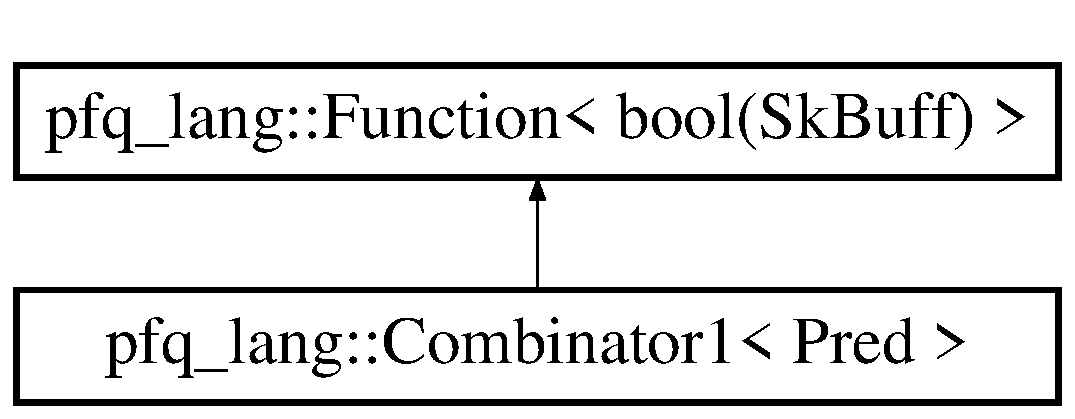
\includegraphics[height=2.000000cm]{structpfq__lang_1_1Combinator1}
\end{center}
\end{figure}
\subsection*{Public Member Functions}
\begin{DoxyCompactItemize}
\item 
\hyperlink{structpfq__lang_1_1Combinator1_a56c94d3734f2976bd0e082d38cf8bd2b}{Combinator1} (std\+::string symbol, Pred p)
\end{DoxyCompactItemize}
\subsection*{Public Attributes}
\begin{DoxyCompactItemize}
\item 
std\+::string \hyperlink{structpfq__lang_1_1Combinator1_addfe327a3bf56ffd84f5c370c5fc3456}{symbol\+\_\+}
\item 
Pred \hyperlink{structpfq__lang_1_1Combinator1_ad4a0a97d1435bd35fe25796a88bbdebf}{pred\+\_\+}
\end{DoxyCompactItemize}
\subsection*{Additional Inherited Members}


\subsection{Constructor \& Destructor Documentation}
\hypertarget{structpfq__lang_1_1Combinator1_a56c94d3734f2976bd0e082d38cf8bd2b}{\index{pfq\+\_\+lang\+::\+Combinator1@{pfq\+\_\+lang\+::\+Combinator1}!Combinator1@{Combinator1}}
\index{Combinator1@{Combinator1}!pfq\+\_\+lang\+::\+Combinator1@{pfq\+\_\+lang\+::\+Combinator1}}
\subsubsection[{Combinator1}]{\setlength{\rightskip}{0pt plus 5cm}template$<$typename Pred$>$ {\bf pfq\+\_\+lang\+::\+Combinator1}$<$ Pred $>$\+::{\bf Combinator1} (
\begin{DoxyParamCaption}
\item[{std\+::string}]{symbol, }
\item[{Pred}]{p}
\end{DoxyParamCaption}
)\hspace{0.3cm}{\ttfamily [inline]}}}\label{structpfq__lang_1_1Combinator1_a56c94d3734f2976bd0e082d38cf8bd2b}


\subsection{Member Data Documentation}
\hypertarget{structpfq__lang_1_1Combinator1_ad4a0a97d1435bd35fe25796a88bbdebf}{\index{pfq\+\_\+lang\+::\+Combinator1@{pfq\+\_\+lang\+::\+Combinator1}!pred\+\_\+@{pred\+\_\+}}
\index{pred\+\_\+@{pred\+\_\+}!pfq\+\_\+lang\+::\+Combinator1@{pfq\+\_\+lang\+::\+Combinator1}}
\subsubsection[{pred\+\_\+}]{\setlength{\rightskip}{0pt plus 5cm}template$<$typename Pred$>$ Pred {\bf pfq\+\_\+lang\+::\+Combinator1}$<$ Pred $>$\+::pred\+\_\+}}\label{structpfq__lang_1_1Combinator1_ad4a0a97d1435bd35fe25796a88bbdebf}
\hypertarget{structpfq__lang_1_1Combinator1_addfe327a3bf56ffd84f5c370c5fc3456}{\index{pfq\+\_\+lang\+::\+Combinator1@{pfq\+\_\+lang\+::\+Combinator1}!symbol\+\_\+@{symbol\+\_\+}}
\index{symbol\+\_\+@{symbol\+\_\+}!pfq\+\_\+lang\+::\+Combinator1@{pfq\+\_\+lang\+::\+Combinator1}}
\subsubsection[{symbol\+\_\+}]{\setlength{\rightskip}{0pt plus 5cm}template$<$typename Pred$>$ std\+::string {\bf pfq\+\_\+lang\+::\+Combinator1}$<$ Pred $>$\+::symbol\+\_\+}}\label{structpfq__lang_1_1Combinator1_addfe327a3bf56ffd84f5c370c5fc3456}


The documentation for this struct was generated from the following file\+:\begin{DoxyCompactItemize}
\item 
C++/pfq-\/lang/\hyperlink{lang_8hpp}{lang.\+hpp}\end{DoxyCompactItemize}

\hypertarget{structpfq__lang_1_1Combinator2}{\section{pfq\+\_\+lang\+:\+:Combinator2$<$ Pred1, Pred2 $>$ Struct Template Reference}
\label{structpfq__lang_1_1Combinator2}\index{pfq\+\_\+lang\+::\+Combinator2$<$ Pred1, Pred2 $>$@{pfq\+\_\+lang\+::\+Combinator2$<$ Pred1, Pred2 $>$}}
}


{\ttfamily \#include $<$lang.\+hpp$>$}

Inheritance diagram for pfq\+\_\+lang\+:\+:Combinator2$<$ Pred1, Pred2 $>$\+:\begin{figure}[H]
\begin{center}
\leavevmode
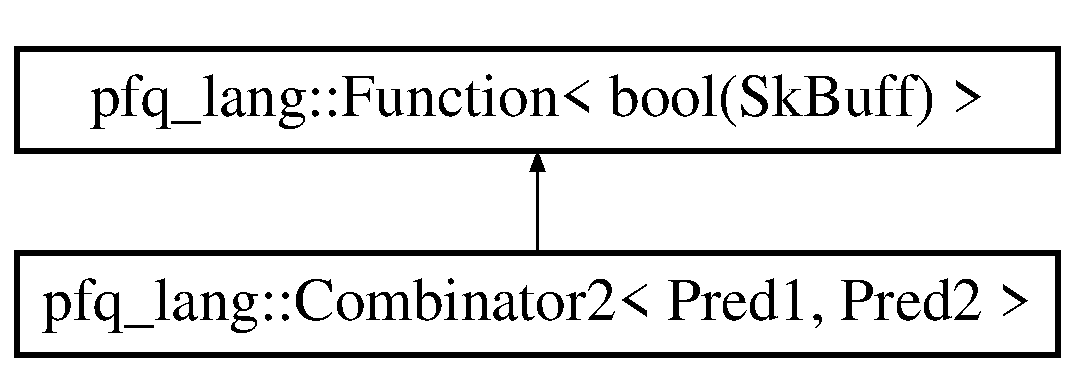
\includegraphics[height=2.000000cm]{structpfq__lang_1_1Combinator2}
\end{center}
\end{figure}
\subsection*{Public Member Functions}
\begin{DoxyCompactItemize}
\item 
\hyperlink{structpfq__lang_1_1Combinator2_a52efcf321388d53ba41d28b6caec515d}{Combinator2} (std\+::string symbol, Pred1 p1, Pred2 p2)
\end{DoxyCompactItemize}
\subsection*{Public Attributes}
\begin{DoxyCompactItemize}
\item 
std\+::string \hyperlink{structpfq__lang_1_1Combinator2_a0fb906403163d6c600b7b86ff915900b}{symbol\+\_\+}
\item 
Pred1 \hyperlink{structpfq__lang_1_1Combinator2_a65f2f5cef67e0525a504529bdb264ab3}{pred1\+\_\+}
\item 
Pred2 \hyperlink{structpfq__lang_1_1Combinator2_a32669787a9dc32693db9813e1e5b7c0d}{pred2\+\_\+}
\end{DoxyCompactItemize}
\subsection*{Additional Inherited Members}


\subsection{Constructor \& Destructor Documentation}
\hypertarget{structpfq__lang_1_1Combinator2_a52efcf321388d53ba41d28b6caec515d}{\index{pfq\+\_\+lang\+::\+Combinator2@{pfq\+\_\+lang\+::\+Combinator2}!Combinator2@{Combinator2}}
\index{Combinator2@{Combinator2}!pfq\+\_\+lang\+::\+Combinator2@{pfq\+\_\+lang\+::\+Combinator2}}
\subsubsection[{Combinator2}]{\setlength{\rightskip}{0pt plus 5cm}template$<$typename Pred1, typename Pred2$>$ {\bf pfq\+\_\+lang\+::\+Combinator2}$<$ Pred1, Pred2 $>$\+::{\bf Combinator2} (
\begin{DoxyParamCaption}
\item[{std\+::string}]{symbol, }
\item[{Pred1}]{p1, }
\item[{Pred2}]{p2}
\end{DoxyParamCaption}
)\hspace{0.3cm}{\ttfamily [inline]}}}\label{structpfq__lang_1_1Combinator2_a52efcf321388d53ba41d28b6caec515d}


\subsection{Member Data Documentation}
\hypertarget{structpfq__lang_1_1Combinator2_a65f2f5cef67e0525a504529bdb264ab3}{\index{pfq\+\_\+lang\+::\+Combinator2@{pfq\+\_\+lang\+::\+Combinator2}!pred1\+\_\+@{pred1\+\_\+}}
\index{pred1\+\_\+@{pred1\+\_\+}!pfq\+\_\+lang\+::\+Combinator2@{pfq\+\_\+lang\+::\+Combinator2}}
\subsubsection[{pred1\+\_\+}]{\setlength{\rightskip}{0pt plus 5cm}template$<$typename Pred1, typename Pred2$>$ Pred1 {\bf pfq\+\_\+lang\+::\+Combinator2}$<$ Pred1, Pred2 $>$\+::pred1\+\_\+}}\label{structpfq__lang_1_1Combinator2_a65f2f5cef67e0525a504529bdb264ab3}
\hypertarget{structpfq__lang_1_1Combinator2_a32669787a9dc32693db9813e1e5b7c0d}{\index{pfq\+\_\+lang\+::\+Combinator2@{pfq\+\_\+lang\+::\+Combinator2}!pred2\+\_\+@{pred2\+\_\+}}
\index{pred2\+\_\+@{pred2\+\_\+}!pfq\+\_\+lang\+::\+Combinator2@{pfq\+\_\+lang\+::\+Combinator2}}
\subsubsection[{pred2\+\_\+}]{\setlength{\rightskip}{0pt plus 5cm}template$<$typename Pred1, typename Pred2$>$ Pred2 {\bf pfq\+\_\+lang\+::\+Combinator2}$<$ Pred1, Pred2 $>$\+::pred2\+\_\+}}\label{structpfq__lang_1_1Combinator2_a32669787a9dc32693db9813e1e5b7c0d}
\hypertarget{structpfq__lang_1_1Combinator2_a0fb906403163d6c600b7b86ff915900b}{\index{pfq\+\_\+lang\+::\+Combinator2@{pfq\+\_\+lang\+::\+Combinator2}!symbol\+\_\+@{symbol\+\_\+}}
\index{symbol\+\_\+@{symbol\+\_\+}!pfq\+\_\+lang\+::\+Combinator2@{pfq\+\_\+lang\+::\+Combinator2}}
\subsubsection[{symbol\+\_\+}]{\setlength{\rightskip}{0pt plus 5cm}template$<$typename Pred1, typename Pred2$>$ std\+::string {\bf pfq\+\_\+lang\+::\+Combinator2}$<$ Pred1, Pred2 $>$\+::symbol\+\_\+}}\label{structpfq__lang_1_1Combinator2_a0fb906403163d6c600b7b86ff915900b}


The documentation for this struct was generated from the following file\+:\begin{DoxyCompactItemize}
\item 
C++/pfq-\/lang/\hyperlink{lang_8hpp}{lang.\+hpp}\end{DoxyCompactItemize}

\hypertarget{structpfq__lang_1_1Composition}{\section{pfq\+\_\+lang\+:\+:Composition$<$ F, G $>$ Struct Template Reference}
\label{structpfq__lang_1_1Composition}\index{pfq\+\_\+lang\+::\+Composition$<$ F, G $>$@{pfq\+\_\+lang\+::\+Composition$<$ F, G $>$}}
}


{\ttfamily \#include $<$lang.\+hpp$>$}

\subsection*{Public Types}
\begin{DoxyCompactItemize}
\item 
using \hyperlink{structpfq__lang_1_1Composition_a60d50413f2357666cec82a4026c87b65}{type} = typename \hyperlink{structpfq__lang_1_1kleisly}{kleisly}$<$ typename F\+::type, typename G\+::type $>$\+::\hyperlink{structpfq__lang_1_1Composition_a60d50413f2357666cec82a4026c87b65}{type}
\end{DoxyCompactItemize}
\subsection*{Public Attributes}
\begin{DoxyCompactItemize}
\item 
F \hyperlink{structpfq__lang_1_1Composition_ac2acb2594f7648731422581b9f2f63b0}{f\+\_\+}
\item 
G \hyperlink{structpfq__lang_1_1Composition_a257ccfaae7168eb34420f23c685f3d41}{g\+\_\+}
\end{DoxyCompactItemize}


\subsection{Member Typedef Documentation}
\hypertarget{structpfq__lang_1_1Composition_a60d50413f2357666cec82a4026c87b65}{\index{pfq\+\_\+lang\+::\+Composition@{pfq\+\_\+lang\+::\+Composition}!type@{type}}
\index{type@{type}!pfq\+\_\+lang\+::\+Composition@{pfq\+\_\+lang\+::\+Composition}}
\subsubsection[{type}]{\setlength{\rightskip}{0pt plus 5cm}template$<$typename F, typename G$>$ using {\bf pfq\+\_\+lang\+::\+Composition}$<$ F, G $>$\+::{\bf type} =  typename {\bf kleisly}$<$typename F\+::type, typename G\+::type$>$\+::{\bf type}}}\label{structpfq__lang_1_1Composition_a60d50413f2357666cec82a4026c87b65}


\subsection{Member Data Documentation}
\hypertarget{structpfq__lang_1_1Composition_ac2acb2594f7648731422581b9f2f63b0}{\index{pfq\+\_\+lang\+::\+Composition@{pfq\+\_\+lang\+::\+Composition}!f\+\_\+@{f\+\_\+}}
\index{f\+\_\+@{f\+\_\+}!pfq\+\_\+lang\+::\+Composition@{pfq\+\_\+lang\+::\+Composition}}
\subsubsection[{f\+\_\+}]{\setlength{\rightskip}{0pt plus 5cm}template$<$typename F, typename G$>$ F {\bf pfq\+\_\+lang\+::\+Composition}$<$ F, G $>$\+::f\+\_\+}}\label{structpfq__lang_1_1Composition_ac2acb2594f7648731422581b9f2f63b0}
\hypertarget{structpfq__lang_1_1Composition_a257ccfaae7168eb34420f23c685f3d41}{\index{pfq\+\_\+lang\+::\+Composition@{pfq\+\_\+lang\+::\+Composition}!g\+\_\+@{g\+\_\+}}
\index{g\+\_\+@{g\+\_\+}!pfq\+\_\+lang\+::\+Composition@{pfq\+\_\+lang\+::\+Composition}}
\subsubsection[{g\+\_\+}]{\setlength{\rightskip}{0pt plus 5cm}template$<$typename F, typename G$>$ G {\bf pfq\+\_\+lang\+::\+Composition}$<$ F, G $>$\+::g\+\_\+}}\label{structpfq__lang_1_1Composition_a257ccfaae7168eb34420f23c685f3d41}


The documentation for this struct was generated from the following file\+:\begin{DoxyCompactItemize}
\item 
C++/pfq-\/lang/\hyperlink{lang_8hpp}{lang.\+hpp}\end{DoxyCompactItemize}

\hypertarget{structpfq__lang_1_1Function}{\section{pfq\+\_\+lang\+:\+:Function$<$ Sig $>$ Struct Template Reference}
\label{structpfq__lang_1_1Function}\index{pfq\+\_\+lang\+::\+Function$<$ Sig $>$@{pfq\+\_\+lang\+::\+Function$<$ Sig $>$}}
}


{\ttfamily \#include $<$lang.\+hpp$>$}

Inheritance diagram for pfq\+\_\+lang\+:\+:Function$<$ Sig $>$\+:\begin{figure}[H]
\begin{center}
\leavevmode
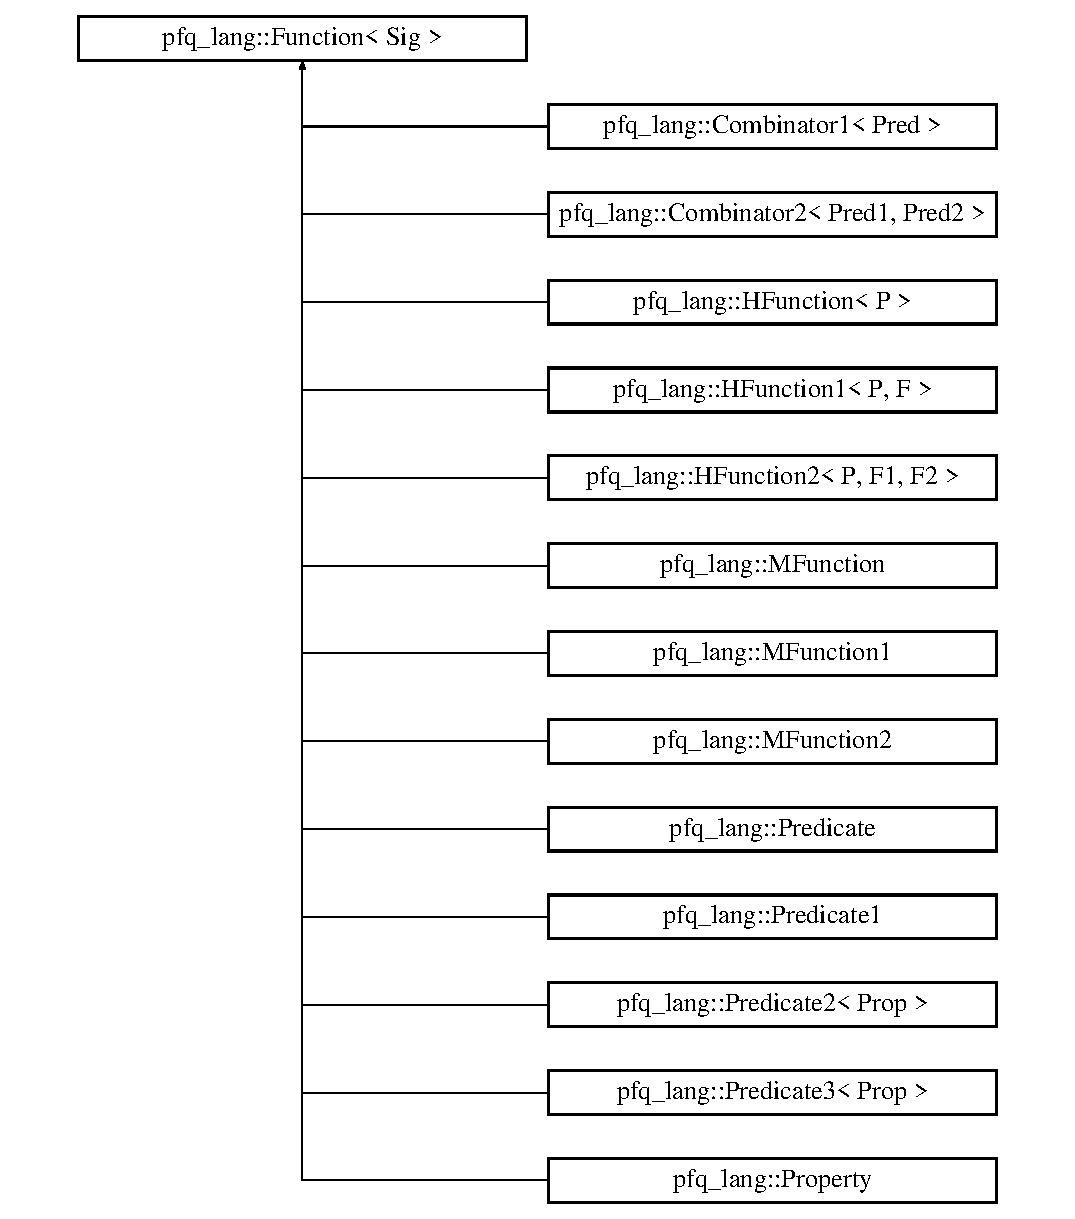
\includegraphics[height=12.000000cm]{structpfq__lang_1_1Function}
\end{center}
\end{figure}
\subsection*{Public Types}
\begin{DoxyCompactItemize}
\item 
using \hyperlink{structpfq__lang_1_1Function_a084321c040f1cec047e0c6ae0c5ec8bd}{type} = \hyperlink{structpfq__lang_1_1Function}{Function}$<$ Sig $>$
\end{DoxyCompactItemize}


\subsection{Member Typedef Documentation}
\hypertarget{structpfq__lang_1_1Function_a084321c040f1cec047e0c6ae0c5ec8bd}{\index{pfq\+\_\+lang\+::\+Function@{pfq\+\_\+lang\+::\+Function}!type@{type}}
\index{type@{type}!pfq\+\_\+lang\+::\+Function@{pfq\+\_\+lang\+::\+Function}}
\subsubsection[{type}]{\setlength{\rightskip}{0pt plus 5cm}template$<$typename Sig $>$ using {\bf pfq\+\_\+lang\+::\+Function}$<$ Sig $>$\+::{\bf type} =  {\bf Function}$<$Sig$>$}}\label{structpfq__lang_1_1Function_a084321c040f1cec047e0c6ae0c5ec8bd}


The documentation for this struct was generated from the following file\+:\begin{DoxyCompactItemize}
\item 
C++/pfq-\/lang/\hyperlink{lang_8hpp}{lang.\+hpp}\end{DoxyCompactItemize}

\hypertarget{structpfq__lang_1_1FunctionDescr}{\section{pfq\+\_\+lang\+:\+:Function\+Descr Struct Reference}
\label{structpfq__lang_1_1FunctionDescr}\index{pfq\+\_\+lang\+::\+Function\+Descr@{pfq\+\_\+lang\+::\+Function\+Descr}}
}


{\ttfamily \#include $<$lang.\+hpp$>$}

\subsection*{Public Attributes}
\begin{DoxyCompactItemize}
\item 
std\+::string \hyperlink{structpfq__lang_1_1FunctionDescr_a58a21262184201b670246fdfdf0cef92}{symbol}
\item 
std\+::array$<$ \hyperlink{structpfq__lang_1_1Argument}{Argument}, 4 $>$ \hyperlink{structpfq__lang_1_1FunctionDescr_a30060a300e3162c65b2bcaf8bde97709}{arg}
\item 
std\+::size\+\_\+t \hyperlink{structpfq__lang_1_1FunctionDescr_abe5a252468a64ff545c4a17b05650744}{next}
\end{DoxyCompactItemize}


\subsection{Member Data Documentation}
\hypertarget{structpfq__lang_1_1FunctionDescr_a30060a300e3162c65b2bcaf8bde97709}{\index{pfq\+\_\+lang\+::\+Function\+Descr@{pfq\+\_\+lang\+::\+Function\+Descr}!arg@{arg}}
\index{arg@{arg}!pfq\+\_\+lang\+::\+Function\+Descr@{pfq\+\_\+lang\+::\+Function\+Descr}}
\subsubsection[{arg}]{\setlength{\rightskip}{0pt plus 5cm}std\+::array$<${\bf Argument}, 4$>$ pfq\+\_\+lang\+::\+Function\+Descr\+::arg}}\label{structpfq__lang_1_1FunctionDescr_a30060a300e3162c65b2bcaf8bde97709}
\hypertarget{structpfq__lang_1_1FunctionDescr_abe5a252468a64ff545c4a17b05650744}{\index{pfq\+\_\+lang\+::\+Function\+Descr@{pfq\+\_\+lang\+::\+Function\+Descr}!next@{next}}
\index{next@{next}!pfq\+\_\+lang\+::\+Function\+Descr@{pfq\+\_\+lang\+::\+Function\+Descr}}
\subsubsection[{next}]{\setlength{\rightskip}{0pt plus 5cm}std\+::size\+\_\+t pfq\+\_\+lang\+::\+Function\+Descr\+::next}}\label{structpfq__lang_1_1FunctionDescr_abe5a252468a64ff545c4a17b05650744}
\hypertarget{structpfq__lang_1_1FunctionDescr_a58a21262184201b670246fdfdf0cef92}{\index{pfq\+\_\+lang\+::\+Function\+Descr@{pfq\+\_\+lang\+::\+Function\+Descr}!symbol@{symbol}}
\index{symbol@{symbol}!pfq\+\_\+lang\+::\+Function\+Descr@{pfq\+\_\+lang\+::\+Function\+Descr}}
\subsubsection[{symbol}]{\setlength{\rightskip}{0pt plus 5cm}std\+::string pfq\+\_\+lang\+::\+Function\+Descr\+::symbol}}\label{structpfq__lang_1_1FunctionDescr_a58a21262184201b670246fdfdf0cef92}


The documentation for this struct was generated from the following file\+:\begin{DoxyCompactItemize}
\item 
C++/pfq-\/lang/\hyperlink{lang_8hpp}{lang.\+hpp}\end{DoxyCompactItemize}

\hypertarget{structpfq__lang_1_1has__insertion__operator}{\section{pfq\+\_\+lang\+:\+:has\+\_\+insertion\+\_\+operator$<$ T $>$ Struct Template Reference}
\label{structpfq__lang_1_1has__insertion__operator}\index{pfq\+\_\+lang\+::has\+\_\+insertion\+\_\+operator$<$ T $>$@{pfq\+\_\+lang\+::has\+\_\+insertion\+\_\+operator$<$ T $>$}}
}


{\ttfamily \#include $<$lang.\+hpp$>$}

Inheritance diagram for pfq\+\_\+lang\+:\+:has\+\_\+insertion\+\_\+operator$<$ T $>$\+:\begin{figure}[H]
\begin{center}
\leavevmode
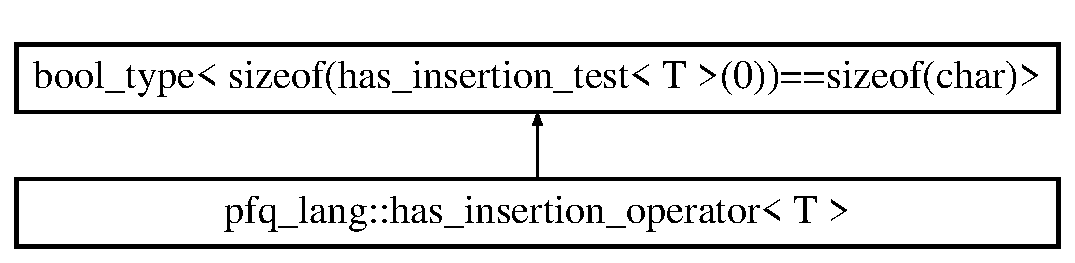
\includegraphics[height=2.000000cm]{structpfq__lang_1_1has__insertion__operator}
\end{center}
\end{figure}


The documentation for this struct was generated from the following file\+:\begin{DoxyCompactItemize}
\item 
C++/pfq-\/lang/\hyperlink{lang_8hpp}{lang.\+hpp}\end{DoxyCompactItemize}

\hypertarget{structpfq__lang_1_1HFunction}{\section{pfq\+\_\+lang\+:\+:H\+Function$<$ P $>$ Struct Template Reference}
\label{structpfq__lang_1_1HFunction}\index{pfq\+\_\+lang\+::\+H\+Function$<$ P $>$@{pfq\+\_\+lang\+::\+H\+Function$<$ P $>$}}
}


{\ttfamily \#include $<$lang.\+hpp$>$}

Inheritance diagram for pfq\+\_\+lang\+:\+:H\+Function$<$ P $>$\+:\begin{figure}[H]
\begin{center}
\leavevmode
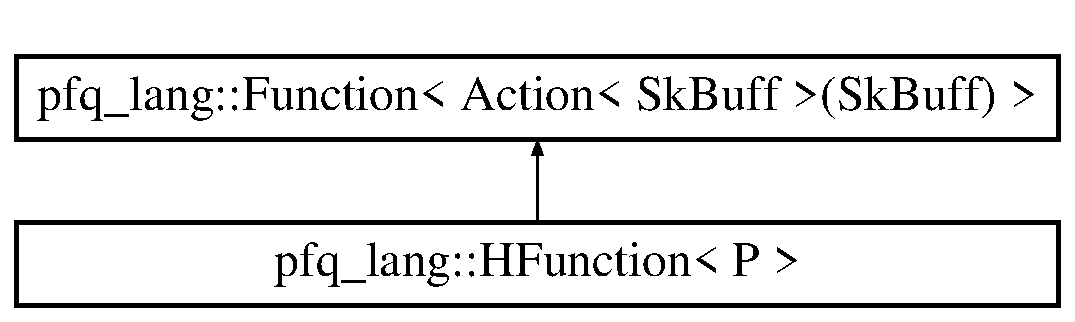
\includegraphics[height=2.000000cm]{structpfq__lang_1_1HFunction}
\end{center}
\end{figure}
\subsection*{Public Member Functions}
\begin{DoxyCompactItemize}
\item 
\hyperlink{structpfq__lang_1_1HFunction_a4cc9560b79a16c4f6c7c7757bd40480c}{H\+Function} (std\+::string symbol, P const \&pred)
\end{DoxyCompactItemize}
\subsection*{Public Attributes}
\begin{DoxyCompactItemize}
\item 
std\+::string \hyperlink{structpfq__lang_1_1HFunction_aaa57a6f399932d77335276b3861c8e08}{symbol\+\_\+}
\item 
P \hyperlink{structpfq__lang_1_1HFunction_abfe7eeab2caa2997c6abb682bf069b8a}{pred\+\_\+}
\end{DoxyCompactItemize}
\subsection*{Additional Inherited Members}


\subsection{Constructor \& Destructor Documentation}
\hypertarget{structpfq__lang_1_1HFunction_a4cc9560b79a16c4f6c7c7757bd40480c}{\index{pfq\+\_\+lang\+::\+H\+Function@{pfq\+\_\+lang\+::\+H\+Function}!H\+Function@{H\+Function}}
\index{H\+Function@{H\+Function}!pfq\+\_\+lang\+::\+H\+Function@{pfq\+\_\+lang\+::\+H\+Function}}
\subsubsection[{H\+Function}]{\setlength{\rightskip}{0pt plus 5cm}template$<$typename P$>$ {\bf pfq\+\_\+lang\+::\+H\+Function}$<$ P $>$\+::{\bf H\+Function} (
\begin{DoxyParamCaption}
\item[{std\+::string}]{symbol, }
\item[{P const \&}]{pred}
\end{DoxyParamCaption}
)\hspace{0.3cm}{\ttfamily [inline]}}}\label{structpfq__lang_1_1HFunction_a4cc9560b79a16c4f6c7c7757bd40480c}


\subsection{Member Data Documentation}
\hypertarget{structpfq__lang_1_1HFunction_abfe7eeab2caa2997c6abb682bf069b8a}{\index{pfq\+\_\+lang\+::\+H\+Function@{pfq\+\_\+lang\+::\+H\+Function}!pred\+\_\+@{pred\+\_\+}}
\index{pred\+\_\+@{pred\+\_\+}!pfq\+\_\+lang\+::\+H\+Function@{pfq\+\_\+lang\+::\+H\+Function}}
\subsubsection[{pred\+\_\+}]{\setlength{\rightskip}{0pt plus 5cm}template$<$typename P$>$ P {\bf pfq\+\_\+lang\+::\+H\+Function}$<$ P $>$\+::pred\+\_\+}}\label{structpfq__lang_1_1HFunction_abfe7eeab2caa2997c6abb682bf069b8a}
\hypertarget{structpfq__lang_1_1HFunction_aaa57a6f399932d77335276b3861c8e08}{\index{pfq\+\_\+lang\+::\+H\+Function@{pfq\+\_\+lang\+::\+H\+Function}!symbol\+\_\+@{symbol\+\_\+}}
\index{symbol\+\_\+@{symbol\+\_\+}!pfq\+\_\+lang\+::\+H\+Function@{pfq\+\_\+lang\+::\+H\+Function}}
\subsubsection[{symbol\+\_\+}]{\setlength{\rightskip}{0pt plus 5cm}template$<$typename P$>$ std\+::string {\bf pfq\+\_\+lang\+::\+H\+Function}$<$ P $>$\+::symbol\+\_\+}}\label{structpfq__lang_1_1HFunction_aaa57a6f399932d77335276b3861c8e08}


The documentation for this struct was generated from the following file\+:\begin{DoxyCompactItemize}
\item 
C++/pfq-\/lang/\hyperlink{lang_8hpp}{lang.\+hpp}\end{DoxyCompactItemize}

\hypertarget{structpfq__lang_1_1HFunction1}{\section{pfq\+\_\+lang\+:\+:H\+Function1$<$ P, F $>$ Struct Template Reference}
\label{structpfq__lang_1_1HFunction1}\index{pfq\+\_\+lang\+::\+H\+Function1$<$ P, F $>$@{pfq\+\_\+lang\+::\+H\+Function1$<$ P, F $>$}}
}


{\ttfamily \#include $<$lang.\+hpp$>$}

Inheritance diagram for pfq\+\_\+lang\+:\+:H\+Function1$<$ P, F $>$\+:\begin{figure}[H]
\begin{center}
\leavevmode
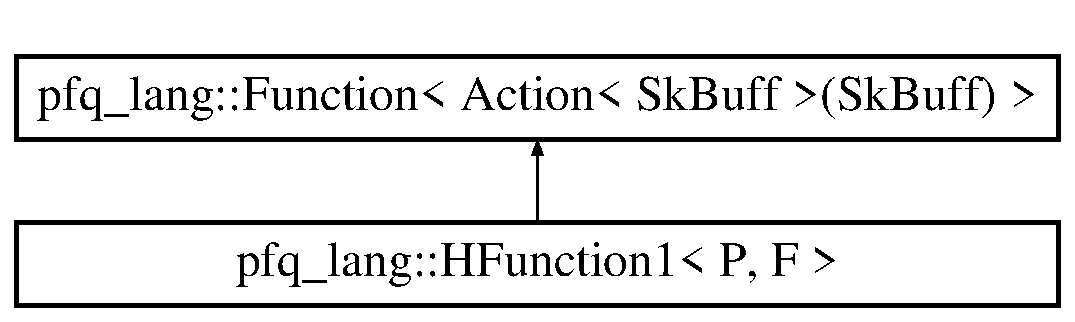
\includegraphics[height=2.000000cm]{structpfq__lang_1_1HFunction1}
\end{center}
\end{figure}
\subsection*{Public Member Functions}
\begin{DoxyCompactItemize}
\item 
\hyperlink{structpfq__lang_1_1HFunction1_ae7edffd30248e1ec3d151326bd3d2cb8}{H\+Function1} (std\+::string symbol, P const \&pred, F const \&fun)
\end{DoxyCompactItemize}
\subsection*{Public Attributes}
\begin{DoxyCompactItemize}
\item 
std\+::string \hyperlink{structpfq__lang_1_1HFunction1_a887acb41567eabcdf4bc02d04b5250ea}{symbol\+\_\+}
\item 
P \hyperlink{structpfq__lang_1_1HFunction1_a2b27dcdb7b9183f330438e650a36aa42}{pred\+\_\+}
\item 
F \hyperlink{structpfq__lang_1_1HFunction1_a24ea2e91b39b0eb547df29785b9a440c}{fun\+\_\+}
\end{DoxyCompactItemize}
\subsection*{Additional Inherited Members}


\subsection{Constructor \& Destructor Documentation}
\hypertarget{structpfq__lang_1_1HFunction1_ae7edffd30248e1ec3d151326bd3d2cb8}{\index{pfq\+\_\+lang\+::\+H\+Function1@{pfq\+\_\+lang\+::\+H\+Function1}!H\+Function1@{H\+Function1}}
\index{H\+Function1@{H\+Function1}!pfq\+\_\+lang\+::\+H\+Function1@{pfq\+\_\+lang\+::\+H\+Function1}}
\subsubsection[{H\+Function1}]{\setlength{\rightskip}{0pt plus 5cm}template$<$typename P, typename F$>$ {\bf pfq\+\_\+lang\+::\+H\+Function1}$<$ P, F $>$\+::{\bf H\+Function1} (
\begin{DoxyParamCaption}
\item[{std\+::string}]{symbol, }
\item[{P const \&}]{pred, }
\item[{F const \&}]{fun}
\end{DoxyParamCaption}
)\hspace{0.3cm}{\ttfamily [inline]}}}\label{structpfq__lang_1_1HFunction1_ae7edffd30248e1ec3d151326bd3d2cb8}


\subsection{Member Data Documentation}
\hypertarget{structpfq__lang_1_1HFunction1_a24ea2e91b39b0eb547df29785b9a440c}{\index{pfq\+\_\+lang\+::\+H\+Function1@{pfq\+\_\+lang\+::\+H\+Function1}!fun\+\_\+@{fun\+\_\+}}
\index{fun\+\_\+@{fun\+\_\+}!pfq\+\_\+lang\+::\+H\+Function1@{pfq\+\_\+lang\+::\+H\+Function1}}
\subsubsection[{fun\+\_\+}]{\setlength{\rightskip}{0pt plus 5cm}template$<$typename P, typename F$>$ F {\bf pfq\+\_\+lang\+::\+H\+Function1}$<$ P, F $>$\+::fun\+\_\+}}\label{structpfq__lang_1_1HFunction1_a24ea2e91b39b0eb547df29785b9a440c}
\hypertarget{structpfq__lang_1_1HFunction1_a2b27dcdb7b9183f330438e650a36aa42}{\index{pfq\+\_\+lang\+::\+H\+Function1@{pfq\+\_\+lang\+::\+H\+Function1}!pred\+\_\+@{pred\+\_\+}}
\index{pred\+\_\+@{pred\+\_\+}!pfq\+\_\+lang\+::\+H\+Function1@{pfq\+\_\+lang\+::\+H\+Function1}}
\subsubsection[{pred\+\_\+}]{\setlength{\rightskip}{0pt plus 5cm}template$<$typename P, typename F$>$ P {\bf pfq\+\_\+lang\+::\+H\+Function1}$<$ P, F $>$\+::pred\+\_\+}}\label{structpfq__lang_1_1HFunction1_a2b27dcdb7b9183f330438e650a36aa42}
\hypertarget{structpfq__lang_1_1HFunction1_a887acb41567eabcdf4bc02d04b5250ea}{\index{pfq\+\_\+lang\+::\+H\+Function1@{pfq\+\_\+lang\+::\+H\+Function1}!symbol\+\_\+@{symbol\+\_\+}}
\index{symbol\+\_\+@{symbol\+\_\+}!pfq\+\_\+lang\+::\+H\+Function1@{pfq\+\_\+lang\+::\+H\+Function1}}
\subsubsection[{symbol\+\_\+}]{\setlength{\rightskip}{0pt plus 5cm}template$<$typename P, typename F$>$ std\+::string {\bf pfq\+\_\+lang\+::\+H\+Function1}$<$ P, F $>$\+::symbol\+\_\+}}\label{structpfq__lang_1_1HFunction1_a887acb41567eabcdf4bc02d04b5250ea}


The documentation for this struct was generated from the following file\+:\begin{DoxyCompactItemize}
\item 
C++/pfq-\/lang/\hyperlink{lang_8hpp}{lang.\+hpp}\end{DoxyCompactItemize}

\hypertarget{structpfq__lang_1_1HFunction2}{\section{pfq\+\_\+lang\+:\+:H\+Function2$<$ P, F1, F2 $>$ Struct Template Reference}
\label{structpfq__lang_1_1HFunction2}\index{pfq\+\_\+lang\+::\+H\+Function2$<$ P, F1, F2 $>$@{pfq\+\_\+lang\+::\+H\+Function2$<$ P, F1, F2 $>$}}
}


{\ttfamily \#include $<$lang.\+hpp$>$}

Inheritance diagram for pfq\+\_\+lang\+:\+:H\+Function2$<$ P, F1, F2 $>$\+:\begin{figure}[H]
\begin{center}
\leavevmode
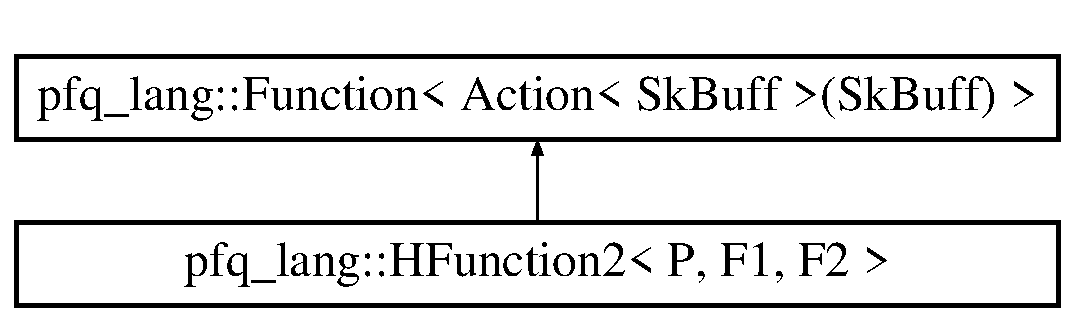
\includegraphics[height=2.000000cm]{structpfq__lang_1_1HFunction2}
\end{center}
\end{figure}
\subsection*{Public Member Functions}
\begin{DoxyCompactItemize}
\item 
\hyperlink{structpfq__lang_1_1HFunction2_a6c0b3bb60f200e7d34876b6b429ab80f}{H\+Function2} (std\+::string symbol, P const \&pred, F const \&fun1, G const \&fun2)
\end{DoxyCompactItemize}
\subsection*{Public Attributes}
\begin{DoxyCompactItemize}
\item 
std\+::string \hyperlink{structpfq__lang_1_1HFunction2_a5c354f72202e280f4e01fa033709da68}{symbol\+\_\+}
\item 
P \hyperlink{structpfq__lang_1_1HFunction2_ab1f1307df8a4b1c23cd9e2905b308679}{pred\+\_\+}
\item 
F \hyperlink{structpfq__lang_1_1HFunction2_a1e7d18cef3f4fce903509c3562369418}{fun1\+\_\+}
\item 
G \hyperlink{structpfq__lang_1_1HFunction2_a55766e7665c4a9f14f9fb5e35ca24405}{fun2\+\_\+}
\end{DoxyCompactItemize}
\subsection*{Additional Inherited Members}


\subsection{Constructor \& Destructor Documentation}
\hypertarget{structpfq__lang_1_1HFunction2_a6c0b3bb60f200e7d34876b6b429ab80f}{\index{pfq\+\_\+lang\+::\+H\+Function2@{pfq\+\_\+lang\+::\+H\+Function2}!H\+Function2@{H\+Function2}}
\index{H\+Function2@{H\+Function2}!pfq\+\_\+lang\+::\+H\+Function2@{pfq\+\_\+lang\+::\+H\+Function2}}
\subsubsection[{H\+Function2}]{\setlength{\rightskip}{0pt plus 5cm}template$<$typename P, typename F1, typename F2$>$ {\bf pfq\+\_\+lang\+::\+H\+Function2}$<$ P, F1, F2 $>$\+::{\bf H\+Function2} (
\begin{DoxyParamCaption}
\item[{std\+::string}]{symbol, }
\item[{P const \&}]{pred, }
\item[{F const \&}]{fun1, }
\item[{G const \&}]{fun2}
\end{DoxyParamCaption}
)\hspace{0.3cm}{\ttfamily [inline]}}}\label{structpfq__lang_1_1HFunction2_a6c0b3bb60f200e7d34876b6b429ab80f}


\subsection{Member Data Documentation}
\hypertarget{structpfq__lang_1_1HFunction2_a1e7d18cef3f4fce903509c3562369418}{\index{pfq\+\_\+lang\+::\+H\+Function2@{pfq\+\_\+lang\+::\+H\+Function2}!fun1\+\_\+@{fun1\+\_\+}}
\index{fun1\+\_\+@{fun1\+\_\+}!pfq\+\_\+lang\+::\+H\+Function2@{pfq\+\_\+lang\+::\+H\+Function2}}
\subsubsection[{fun1\+\_\+}]{\setlength{\rightskip}{0pt plus 5cm}template$<$typename P, typename F1, typename F2$>$ F {\bf pfq\+\_\+lang\+::\+H\+Function2}$<$ P, F1, F2 $>$\+::fun1\+\_\+}}\label{structpfq__lang_1_1HFunction2_a1e7d18cef3f4fce903509c3562369418}
\hypertarget{structpfq__lang_1_1HFunction2_a55766e7665c4a9f14f9fb5e35ca24405}{\index{pfq\+\_\+lang\+::\+H\+Function2@{pfq\+\_\+lang\+::\+H\+Function2}!fun2\+\_\+@{fun2\+\_\+}}
\index{fun2\+\_\+@{fun2\+\_\+}!pfq\+\_\+lang\+::\+H\+Function2@{pfq\+\_\+lang\+::\+H\+Function2}}
\subsubsection[{fun2\+\_\+}]{\setlength{\rightskip}{0pt plus 5cm}template$<$typename P, typename F1, typename F2$>$ G {\bf pfq\+\_\+lang\+::\+H\+Function2}$<$ P, F1, F2 $>$\+::fun2\+\_\+}}\label{structpfq__lang_1_1HFunction2_a55766e7665c4a9f14f9fb5e35ca24405}
\hypertarget{structpfq__lang_1_1HFunction2_ab1f1307df8a4b1c23cd9e2905b308679}{\index{pfq\+\_\+lang\+::\+H\+Function2@{pfq\+\_\+lang\+::\+H\+Function2}!pred\+\_\+@{pred\+\_\+}}
\index{pred\+\_\+@{pred\+\_\+}!pfq\+\_\+lang\+::\+H\+Function2@{pfq\+\_\+lang\+::\+H\+Function2}}
\subsubsection[{pred\+\_\+}]{\setlength{\rightskip}{0pt plus 5cm}template$<$typename P, typename F1, typename F2$>$ P {\bf pfq\+\_\+lang\+::\+H\+Function2}$<$ P, F1, F2 $>$\+::pred\+\_\+}}\label{structpfq__lang_1_1HFunction2_ab1f1307df8a4b1c23cd9e2905b308679}
\hypertarget{structpfq__lang_1_1HFunction2_a5c354f72202e280f4e01fa033709da68}{\index{pfq\+\_\+lang\+::\+H\+Function2@{pfq\+\_\+lang\+::\+H\+Function2}!symbol\+\_\+@{symbol\+\_\+}}
\index{symbol\+\_\+@{symbol\+\_\+}!pfq\+\_\+lang\+::\+H\+Function2@{pfq\+\_\+lang\+::\+H\+Function2}}
\subsubsection[{symbol\+\_\+}]{\setlength{\rightskip}{0pt plus 5cm}template$<$typename P, typename F1, typename F2$>$ std\+::string {\bf pfq\+\_\+lang\+::\+H\+Function2}$<$ P, F1, F2 $>$\+::symbol\+\_\+}}\label{structpfq__lang_1_1HFunction2_a5c354f72202e280f4e01fa033709da68}


The documentation for this struct was generated from the following file\+:\begin{DoxyCompactItemize}
\item 
C++/pfq-\/lang/\hyperlink{lang_8hpp}{lang.\+hpp}\end{DoxyCompactItemize}

\hypertarget{structpfq__lang_1_1HFunction3}{\section{pfq\+\_\+lang\+:\+:H\+Function3$<$ F $>$ Struct Template Reference}
\label{structpfq__lang_1_1HFunction3}\index{pfq\+\_\+lang\+::\+H\+Function3$<$ F $>$@{pfq\+\_\+lang\+::\+H\+Function3$<$ F $>$}}
}


{\ttfamily \#include $<$lang.\+hpp$>$}

Inheritance diagram for pfq\+\_\+lang\+:\+:H\+Function3$<$ F $>$\+:\begin{figure}[H]
\begin{center}
\leavevmode
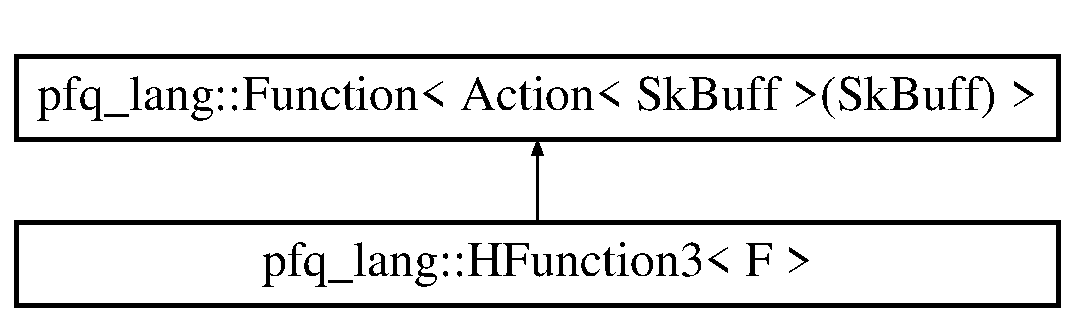
\includegraphics[height=2.000000cm]{structpfq__lang_1_1HFunction3}
\end{center}
\end{figure}
\subsection*{Public Member Functions}
\begin{DoxyCompactItemize}
\item 
\hyperlink{structpfq__lang_1_1HFunction3_ae3e015cd8bcc99f4b1c3b38367964371}{H\+Function3} (std\+::string symbol, F const \&fun)
\end{DoxyCompactItemize}
\subsection*{Public Attributes}
\begin{DoxyCompactItemize}
\item 
std\+::string \hyperlink{structpfq__lang_1_1HFunction3_ae0ba31689b517305a696401dbd63bd31}{symbol\+\_\+}
\item 
F \hyperlink{structpfq__lang_1_1HFunction3_ab7ac85c47b00236fa5d8dbd268669770}{fun\+\_\+}
\end{DoxyCompactItemize}
\subsection*{Additional Inherited Members}


\subsection{Constructor \& Destructor Documentation}
\hypertarget{structpfq__lang_1_1HFunction3_ae3e015cd8bcc99f4b1c3b38367964371}{\index{pfq\+\_\+lang\+::\+H\+Function3@{pfq\+\_\+lang\+::\+H\+Function3}!H\+Function3@{H\+Function3}}
\index{H\+Function3@{H\+Function3}!pfq\+\_\+lang\+::\+H\+Function3@{pfq\+\_\+lang\+::\+H\+Function3}}
\subsubsection[{H\+Function3}]{\setlength{\rightskip}{0pt plus 5cm}template$<$typename F$>$ {\bf pfq\+\_\+lang\+::\+H\+Function3}$<$ F $>$\+::{\bf H\+Function3} (
\begin{DoxyParamCaption}
\item[{std\+::string}]{symbol, }
\item[{F const \&}]{fun}
\end{DoxyParamCaption}
)\hspace{0.3cm}{\ttfamily [inline]}}}\label{structpfq__lang_1_1HFunction3_ae3e015cd8bcc99f4b1c3b38367964371}


\subsection{Member Data Documentation}
\hypertarget{structpfq__lang_1_1HFunction3_ab7ac85c47b00236fa5d8dbd268669770}{\index{pfq\+\_\+lang\+::\+H\+Function3@{pfq\+\_\+lang\+::\+H\+Function3}!fun\+\_\+@{fun\+\_\+}}
\index{fun\+\_\+@{fun\+\_\+}!pfq\+\_\+lang\+::\+H\+Function3@{pfq\+\_\+lang\+::\+H\+Function3}}
\subsubsection[{fun\+\_\+}]{\setlength{\rightskip}{0pt plus 5cm}template$<$typename F$>$ F {\bf pfq\+\_\+lang\+::\+H\+Function3}$<$ F $>$\+::fun\+\_\+}}\label{structpfq__lang_1_1HFunction3_ab7ac85c47b00236fa5d8dbd268669770}
\hypertarget{structpfq__lang_1_1HFunction3_ae0ba31689b517305a696401dbd63bd31}{\index{pfq\+\_\+lang\+::\+H\+Function3@{pfq\+\_\+lang\+::\+H\+Function3}!symbol\+\_\+@{symbol\+\_\+}}
\index{symbol\+\_\+@{symbol\+\_\+}!pfq\+\_\+lang\+::\+H\+Function3@{pfq\+\_\+lang\+::\+H\+Function3}}
\subsubsection[{symbol\+\_\+}]{\setlength{\rightskip}{0pt plus 5cm}template$<$typename F$>$ std\+::string {\bf pfq\+\_\+lang\+::\+H\+Function3}$<$ F $>$\+::symbol\+\_\+}}\label{structpfq__lang_1_1HFunction3_ae0ba31689b517305a696401dbd63bd31}


The documentation for this struct was generated from the following file\+:\begin{DoxyCompactItemize}
\item 
C++/pfq-\/lang/\hyperlink{lang_8hpp}{lang.\+hpp}\end{DoxyCompactItemize}

\hypertarget{structpfq__lang_1_1HFunction4}{\section{pfq\+\_\+lang\+:\+:H\+Function4$<$ F, G $>$ Struct Template Reference}
\label{structpfq__lang_1_1HFunction4}\index{pfq\+\_\+lang\+::\+H\+Function4$<$ F, G $>$@{pfq\+\_\+lang\+::\+H\+Function4$<$ F, G $>$}}
}


{\ttfamily \#include $<$lang.\+hpp$>$}

Inheritance diagram for pfq\+\_\+lang\+:\+:H\+Function4$<$ F, G $>$\+:\begin{figure}[H]
\begin{center}
\leavevmode
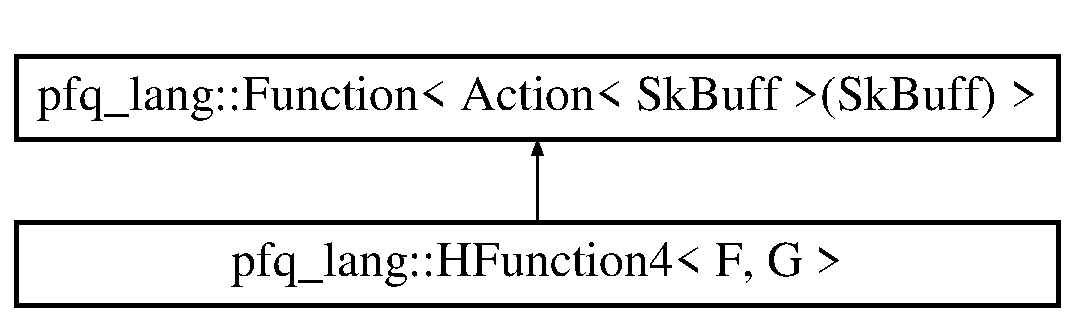
\includegraphics[height=2.000000cm]{structpfq__lang_1_1HFunction4}
\end{center}
\end{figure}
\subsection*{Public Member Functions}
\begin{DoxyCompactItemize}
\item 
\hyperlink{structpfq__lang_1_1HFunction4_abc43b6b36341cd71c4d6a6de0d7265dc}{H\+Function4} (std\+::string symbol, F const \&f, G const \&g)
\end{DoxyCompactItemize}
\subsection*{Public Attributes}
\begin{DoxyCompactItemize}
\item 
std\+::string \hyperlink{structpfq__lang_1_1HFunction4_ad58dbdba4ab08dc0d78cce96f16b02c5}{symbol\+\_\+}
\item 
F \hyperlink{structpfq__lang_1_1HFunction4_a4a05b28c32d35ba19353d5c7fe028aa0}{f\+\_\+}
\item 
G \hyperlink{structpfq__lang_1_1HFunction4_ad7cf948fb1775430924e0a46dece3d12}{g\+\_\+}
\end{DoxyCompactItemize}
\subsection*{Additional Inherited Members}


\subsection{Constructor \& Destructor Documentation}
\hypertarget{structpfq__lang_1_1HFunction4_abc43b6b36341cd71c4d6a6de0d7265dc}{\index{pfq\+\_\+lang\+::\+H\+Function4@{pfq\+\_\+lang\+::\+H\+Function4}!H\+Function4@{H\+Function4}}
\index{H\+Function4@{H\+Function4}!pfq\+\_\+lang\+::\+H\+Function4@{pfq\+\_\+lang\+::\+H\+Function4}}
\subsubsection[{H\+Function4}]{\setlength{\rightskip}{0pt plus 5cm}template$<$typename F, typename G$>$ {\bf pfq\+\_\+lang\+::\+H\+Function4}$<$ F, G $>$\+::{\bf H\+Function4} (
\begin{DoxyParamCaption}
\item[{std\+::string}]{symbol, }
\item[{F const \&}]{f, }
\item[{G const \&}]{g}
\end{DoxyParamCaption}
)\hspace{0.3cm}{\ttfamily [inline]}}}\label{structpfq__lang_1_1HFunction4_abc43b6b36341cd71c4d6a6de0d7265dc}


\subsection{Member Data Documentation}
\hypertarget{structpfq__lang_1_1HFunction4_a4a05b28c32d35ba19353d5c7fe028aa0}{\index{pfq\+\_\+lang\+::\+H\+Function4@{pfq\+\_\+lang\+::\+H\+Function4}!f\+\_\+@{f\+\_\+}}
\index{f\+\_\+@{f\+\_\+}!pfq\+\_\+lang\+::\+H\+Function4@{pfq\+\_\+lang\+::\+H\+Function4}}
\subsubsection[{f\+\_\+}]{\setlength{\rightskip}{0pt plus 5cm}template$<$typename F, typename G$>$ F {\bf pfq\+\_\+lang\+::\+H\+Function4}$<$ F, G $>$\+::f\+\_\+}}\label{structpfq__lang_1_1HFunction4_a4a05b28c32d35ba19353d5c7fe028aa0}
\hypertarget{structpfq__lang_1_1HFunction4_ad7cf948fb1775430924e0a46dece3d12}{\index{pfq\+\_\+lang\+::\+H\+Function4@{pfq\+\_\+lang\+::\+H\+Function4}!g\+\_\+@{g\+\_\+}}
\index{g\+\_\+@{g\+\_\+}!pfq\+\_\+lang\+::\+H\+Function4@{pfq\+\_\+lang\+::\+H\+Function4}}
\subsubsection[{g\+\_\+}]{\setlength{\rightskip}{0pt plus 5cm}template$<$typename F, typename G$>$ G {\bf pfq\+\_\+lang\+::\+H\+Function4}$<$ F, G $>$\+::g\+\_\+}}\label{structpfq__lang_1_1HFunction4_ad7cf948fb1775430924e0a46dece3d12}
\hypertarget{structpfq__lang_1_1HFunction4_ad58dbdba4ab08dc0d78cce96f16b02c5}{\index{pfq\+\_\+lang\+::\+H\+Function4@{pfq\+\_\+lang\+::\+H\+Function4}!symbol\+\_\+@{symbol\+\_\+}}
\index{symbol\+\_\+@{symbol\+\_\+}!pfq\+\_\+lang\+::\+H\+Function4@{pfq\+\_\+lang\+::\+H\+Function4}}
\subsubsection[{symbol\+\_\+}]{\setlength{\rightskip}{0pt plus 5cm}template$<$typename F, typename G$>$ std\+::string {\bf pfq\+\_\+lang\+::\+H\+Function4}$<$ F, G $>$\+::symbol\+\_\+}}\label{structpfq__lang_1_1HFunction4_ad58dbdba4ab08dc0d78cce96f16b02c5}


The documentation for this struct was generated from the following file\+:\begin{DoxyCompactItemize}
\item 
C++/pfq-\/lang/\hyperlink{lang_8hpp}{lang.\+hpp}\end{DoxyCompactItemize}

\hypertarget{structpfq__lang_1_1is__Function}{\section{pfq\+\_\+lang\+:\+:is\+\_\+\+Function$<$ Tp $>$ Struct Template Reference}
\label{structpfq__lang_1_1is__Function}\index{pfq\+\_\+lang\+::is\+\_\+\+Function$<$ Tp $>$@{pfq\+\_\+lang\+::is\+\_\+\+Function$<$ Tp $>$}}
}


{\ttfamily \#include $<$lang.\+hpp$>$}

Inheritance diagram for pfq\+\_\+lang\+:\+:is\+\_\+\+Function$<$ Tp $>$\+:\begin{figure}[H]
\begin{center}
\leavevmode
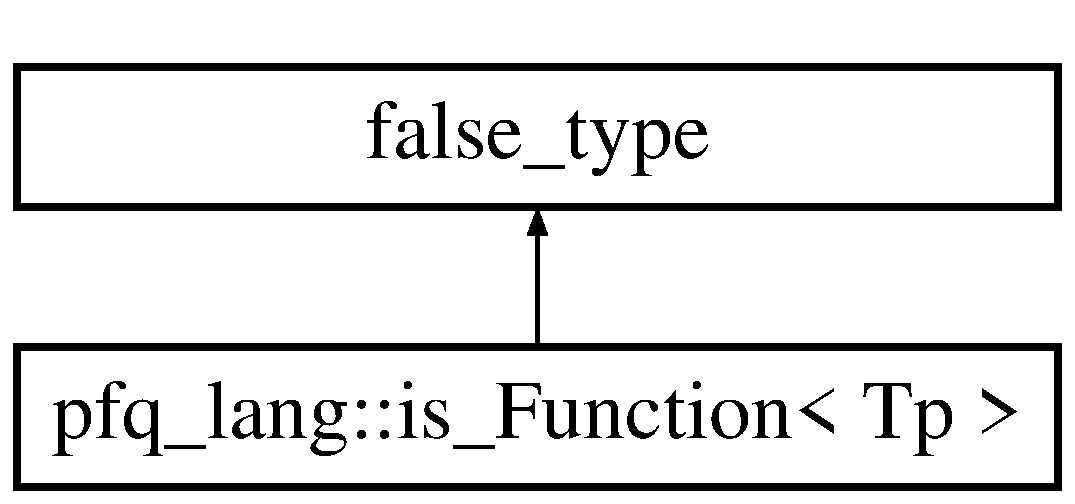
\includegraphics[height=2.000000cm]{structpfq__lang_1_1is__Function}
\end{center}
\end{figure}


The documentation for this struct was generated from the following file\+:\begin{DoxyCompactItemize}
\item 
C++/pfq-\/lang/\hyperlink{lang_8hpp}{lang.\+hpp}\end{DoxyCompactItemize}

\hypertarget{structpfq__lang_1_1is__Function_3_01Function_3_01S_01_4_01_4}{\section{pfq\+\_\+lang\+:\+:is\+\_\+\+Function$<$ Function$<$ S $>$ $>$ Struct Template Reference}
\label{structpfq__lang_1_1is__Function_3_01Function_3_01S_01_4_01_4}\index{pfq\+\_\+lang\+::is\+\_\+\+Function$<$ Function$<$ S $>$ $>$@{pfq\+\_\+lang\+::is\+\_\+\+Function$<$ Function$<$ S $>$ $>$}}
}


{\ttfamily \#include $<$lang.\+hpp$>$}

Inheritance diagram for pfq\+\_\+lang\+:\+:is\+\_\+\+Function$<$ Function$<$ S $>$ $>$\+:\begin{figure}[H]
\begin{center}
\leavevmode
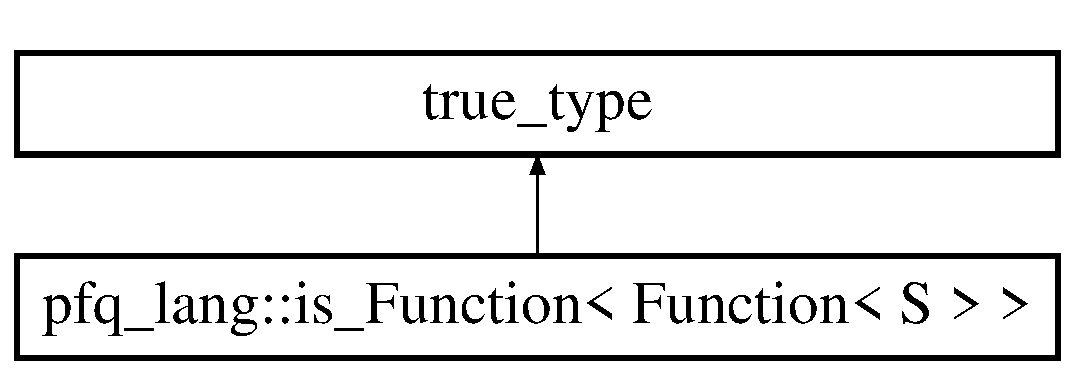
\includegraphics[height=2.000000cm]{structpfq__lang_1_1is__Function_3_01Function_3_01S_01_4_01_4}
\end{center}
\end{figure}


The documentation for this struct was generated from the following file\+:\begin{DoxyCompactItemize}
\item 
C++/pfq-\/lang/\hyperlink{lang_8hpp}{lang.\+hpp}\end{DoxyCompactItemize}

\hypertarget{structpfq__lang_1_1is__mfunction}{\section{pfq\+\_\+lang\+:\+:is\+\_\+mfunction$<$ Tp $>$ Struct Template Reference}
\label{structpfq__lang_1_1is__mfunction}\index{pfq\+\_\+lang\+::is\+\_\+mfunction$<$ Tp $>$@{pfq\+\_\+lang\+::is\+\_\+mfunction$<$ Tp $>$}}
}


{\ttfamily \#include $<$lang.\+hpp$>$}

Inheritance diagram for pfq\+\_\+lang\+:\+:is\+\_\+mfunction$<$ Tp $>$\+:\begin{figure}[H]
\begin{center}
\leavevmode
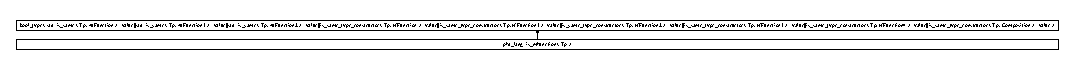
\includegraphics[height=0.436477cm]{structpfq__lang_1_1is__mfunction}
\end{center}
\end{figure}


The documentation for this struct was generated from the following file\+:\begin{DoxyCompactItemize}
\item 
C++/pfq-\/lang/\hyperlink{lang_8hpp}{lang.\+hpp}\end{DoxyCompactItemize}

\hypertarget{structpfq__lang_1_1is__predicate}{\section{pfq\+\_\+lang\+:\+:is\+\_\+predicate$<$ Tp $>$ Struct Template Reference}
\label{structpfq__lang_1_1is__predicate}\index{pfq\+\_\+lang\+::is\+\_\+predicate$<$ Tp $>$@{pfq\+\_\+lang\+::is\+\_\+predicate$<$ Tp $>$}}
}


{\ttfamily \#include $<$lang.\+hpp$>$}

Inheritance diagram for pfq\+\_\+lang\+:\+:is\+\_\+predicate$<$ Tp $>$\+:\begin{figure}[H]
\begin{center}
\leavevmode
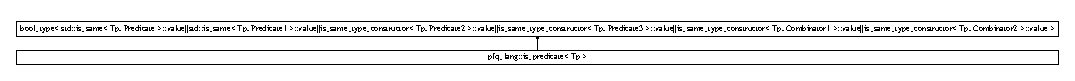
\includegraphics[height=0.645905cm]{structpfq__lang_1_1is__predicate}
\end{center}
\end{figure}


The documentation for this struct was generated from the following file\+:\begin{DoxyCompactItemize}
\item 
C++/pfq-\/lang/\hyperlink{lang_8hpp}{lang.\+hpp}\end{DoxyCompactItemize}

\hypertarget{structpfq__lang_1_1is__property}{\section{pfq\+\_\+lang\+:\+:is\+\_\+property$<$ Tp $>$ Struct Template Reference}
\label{structpfq__lang_1_1is__property}\index{pfq\+\_\+lang\+::is\+\_\+property$<$ Tp $>$@{pfq\+\_\+lang\+::is\+\_\+property$<$ Tp $>$}}
}


{\ttfamily \#include $<$lang.\+hpp$>$}

Inheritance diagram for pfq\+\_\+lang\+:\+:is\+\_\+property$<$ Tp $>$\+:\begin{figure}[H]
\begin{center}
\leavevmode
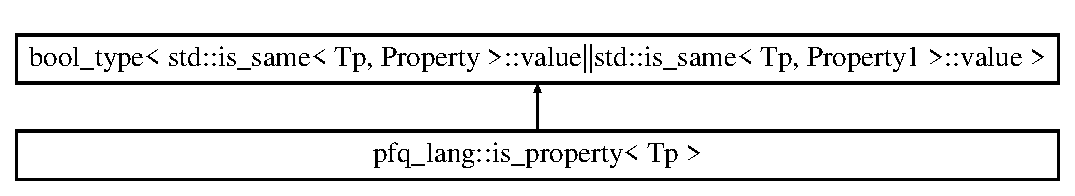
\includegraphics[height=2.000000cm]{structpfq__lang_1_1is__property}
\end{center}
\end{figure}


The documentation for this struct was generated from the following file\+:\begin{DoxyCompactItemize}
\item 
C++/pfq-\/lang/\hyperlink{lang_8hpp}{lang.\+hpp}\end{DoxyCompactItemize}

\hypertarget{structpfq__lang_1_1is__same__type__constructor}{\section{pfq\+\_\+lang\+:\+:is\+\_\+same\+\_\+type\+\_\+constructor$<$ T, Tp $>$ Struct Template Reference}
\label{structpfq__lang_1_1is__same__type__constructor}\index{pfq\+\_\+lang\+::is\+\_\+same\+\_\+type\+\_\+constructor$<$ T, Tp $>$@{pfq\+\_\+lang\+::is\+\_\+same\+\_\+type\+\_\+constructor$<$ T, Tp $>$}}
}


{\ttfamily \#include $<$lang.\+hpp$>$}

Inheritance diagram for pfq\+\_\+lang\+:\+:is\+\_\+same\+\_\+type\+\_\+constructor$<$ T, Tp $>$\+:\begin{figure}[H]
\begin{center}
\leavevmode
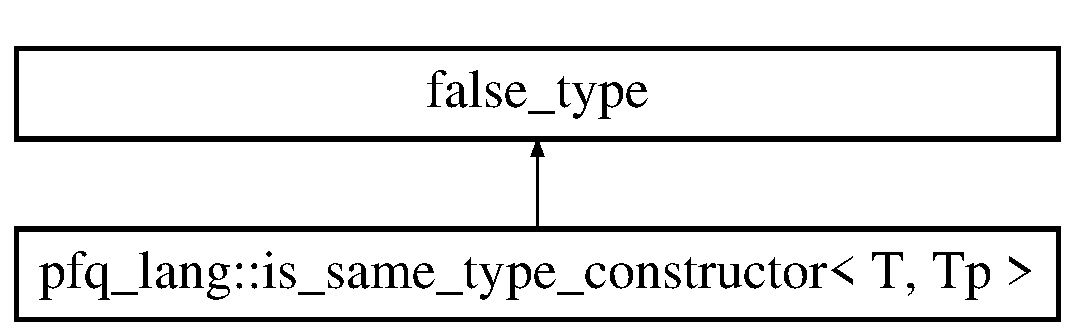
\includegraphics[height=2.000000cm]{structpfq__lang_1_1is__same__type__constructor}
\end{center}
\end{figure}


The documentation for this struct was generated from the following file\+:\begin{DoxyCompactItemize}
\item 
C++/pfq-\/lang/\hyperlink{lang_8hpp}{lang.\+hpp}\end{DoxyCompactItemize}

\hypertarget{structpfq__lang_1_1is__same__type__constructor_3_01Tp_3_01Ti_8_8_8_4_00_01Tp_01_4}{\section{pfq\+\_\+lang\+:\+:is\+\_\+same\+\_\+type\+\_\+constructor$<$ Tp$<$ Ti...$>$, Tp $>$ Struct Template Reference}
\label{structpfq__lang_1_1is__same__type__constructor_3_01Tp_3_01Ti_8_8_8_4_00_01Tp_01_4}\index{pfq\+\_\+lang\+::is\+\_\+same\+\_\+type\+\_\+constructor$<$ Tp$<$ Ti...$>$, Tp $>$@{pfq\+\_\+lang\+::is\+\_\+same\+\_\+type\+\_\+constructor$<$ Tp$<$ Ti...$>$, Tp $>$}}
}


{\ttfamily \#include $<$lang.\+hpp$>$}

Inheritance diagram for pfq\+\_\+lang\+:\+:is\+\_\+same\+\_\+type\+\_\+constructor$<$ Tp$<$ Ti...$>$, Tp $>$\+:\begin{figure}[H]
\begin{center}
\leavevmode
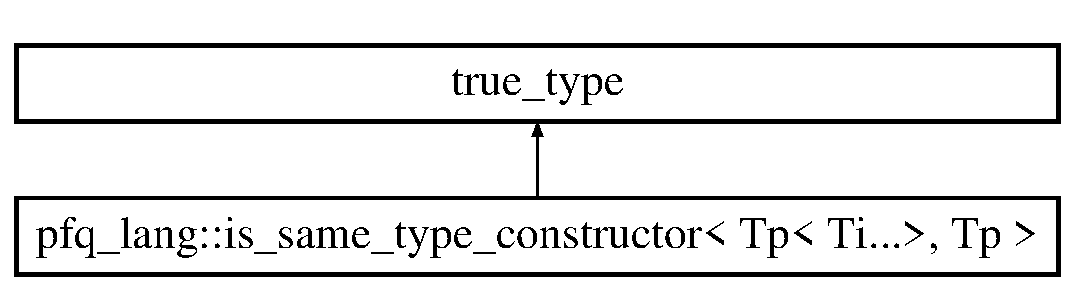
\includegraphics[height=2.000000cm]{structpfq__lang_1_1is__same__type__constructor_3_01Tp_3_01Ti_8_8_8_4_00_01Tp_01_4}
\end{center}
\end{figure}


The documentation for this struct was generated from the following file\+:\begin{DoxyCompactItemize}
\item 
C++/pfq-\/lang/\hyperlink{lang_8hpp}{lang.\+hpp}\end{DoxyCompactItemize}

\hypertarget{structpfq__lang_1_1kleisly}{\section{pfq\+\_\+lang\+:\+:kleisly$<$ F, G $>$ Struct Template Reference}
\label{structpfq__lang_1_1kleisly}\index{pfq\+\_\+lang\+::kleisly$<$ F, G $>$@{pfq\+\_\+lang\+::kleisly$<$ F, G $>$}}
}


{\ttfamily \#include $<$lang.\+hpp$>$}



The documentation for this struct was generated from the following file\+:\begin{DoxyCompactItemize}
\item 
C++/pfq-\/lang/\hyperlink{lang_8hpp}{lang.\+hpp}\end{DoxyCompactItemize}

\hypertarget{structpfq__lang_1_1kleisly_3_01Function_3_01M_3_01B_01_4_07A_08_01_4_00_01Composition_3_01F_00_01G_01_4_01_4}{\section{pfq\+\_\+lang\+:\+:kleisly$<$ Function$<$ M$<$ B $>$(A) $>$, Composition$<$ F, G $>$ $>$ Struct Template Reference}
\label{structpfq__lang_1_1kleisly_3_01Function_3_01M_3_01B_01_4_07A_08_01_4_00_01Composition_3_01F_00_01G_01_4_01_4}\index{pfq\+\_\+lang\+::kleisly$<$ Function$<$ M$<$ B $>$(\+A) $>$, Composition$<$ F, G $>$ $>$@{pfq\+\_\+lang\+::kleisly$<$ Function$<$ M$<$ B $>$(\+A) $>$, Composition$<$ F, G $>$ $>$}}
}


{\ttfamily \#include $<$lang.\+hpp$>$}

\subsection*{Public Types}
\begin{DoxyCompactItemize}
\item 
using \hyperlink{structpfq__lang_1_1kleisly_3_01Function_3_01M_3_01B_01_4_07A_08_01_4_00_01Composition_3_01F_00_01G_01_4_01_4_a73a71a99f99e69b49591eaab1f358e18}{type} = typename \hyperlink{structpfq__lang_1_1kleisly}{kleisly}$<$ \hyperlink{structpfq__lang_1_1Function}{Function}$<$ M$<$ B $>$(A)$>$, typename \hyperlink{structpfq__lang_1_1kleisly}{kleisly}$<$ F, G $>$\+::\hyperlink{structpfq__lang_1_1kleisly_3_01Function_3_01M_3_01B_01_4_07A_08_01_4_00_01Composition_3_01F_00_01G_01_4_01_4_a73a71a99f99e69b49591eaab1f358e18}{type} $>$\+::\hyperlink{structpfq__lang_1_1kleisly_3_01Function_3_01M_3_01B_01_4_07A_08_01_4_00_01Composition_3_01F_00_01G_01_4_01_4_a73a71a99f99e69b49591eaab1f358e18}{type}
\end{DoxyCompactItemize}


\subsection{Member Typedef Documentation}
\hypertarget{structpfq__lang_1_1kleisly_3_01Function_3_01M_3_01B_01_4_07A_08_01_4_00_01Composition_3_01F_00_01G_01_4_01_4_a73a71a99f99e69b49591eaab1f358e18}{\index{pfq\+\_\+lang\+::kleisly$<$ Function$<$ M$<$ B $>$(\+A) $>$, Composition$<$ F, G $>$ $>$@{pfq\+\_\+lang\+::kleisly$<$ Function$<$ M$<$ B $>$(\+A) $>$, Composition$<$ F, G $>$ $>$}!type@{type}}
\index{type@{type}!pfq\+\_\+lang\+::kleisly$<$ Function$<$ M$<$ B $>$(\+A) $>$, Composition$<$ F, G $>$ $>$@{pfq\+\_\+lang\+::kleisly$<$ Function$<$ M$<$ B $>$(\+A) $>$, Composition$<$ F, G $>$ $>$}}
\subsubsection[{type}]{\setlength{\rightskip}{0pt plus 5cm}template$<$template$<$ typename $>$ class M, typename A , typename B , typename F , typename G $>$ using {\bf pfq\+\_\+lang\+::kleisly}$<$ {\bf Function}$<$ M$<$ B $>$(A) $>$, {\bf Composition}$<$ F, G $>$ $>$\+::{\bf type} =  typename {\bf kleisly}$<$ {\bf Function}$<$M$<$B$>$(A)$>$, typename {\bf kleisly}$<$F,G$>$\+::{\bf type}$>$\+::{\bf type}}}\label{structpfq__lang_1_1kleisly_3_01Function_3_01M_3_01B_01_4_07A_08_01_4_00_01Composition_3_01F_00_01G_01_4_01_4_a73a71a99f99e69b49591eaab1f358e18}


The documentation for this struct was generated from the following file\+:\begin{DoxyCompactItemize}
\item 
C++/pfq-\/lang/\hyperlink{lang_8hpp}{lang.\+hpp}\end{DoxyCompactItemize}

\hypertarget{structpfq__lang_1_1kleisly_3_01Function_3_01M_3_01B_01_4_07A_08_01_4_00_01Function_3_01M_3_01C_01_4_07B_08_4_01_4}{\section{pfq\+\_\+lang\+:\+:kleisly$<$ Function$<$ M$<$ B $>$(A) $>$, Function$<$ M$<$ C $>$(B)$>$ $>$ Struct Template Reference}
\label{structpfq__lang_1_1kleisly_3_01Function_3_01M_3_01B_01_4_07A_08_01_4_00_01Function_3_01M_3_01C_01_4_07B_08_4_01_4}\index{pfq\+\_\+lang\+::kleisly$<$ Function$<$ M$<$ B $>$(\+A) $>$, Function$<$ M$<$ C $>$(\+B)$>$ $>$@{pfq\+\_\+lang\+::kleisly$<$ Function$<$ M$<$ B $>$(\+A) $>$, Function$<$ M$<$ C $>$(\+B)$>$ $>$}}
}


{\ttfamily \#include $<$lang.\+hpp$>$}

\subsection*{Public Types}
\begin{DoxyCompactItemize}
\item 
using \hyperlink{structpfq__lang_1_1kleisly_3_01Function_3_01M_3_01B_01_4_07A_08_01_4_00_01Function_3_01M_3_01C_01_4_07B_08_4_01_4_a9a202c30484a455c38a3632c5eee4c47}{type} = \hyperlink{structpfq__lang_1_1Function}{Function}$<$ M$<$ C $>$(A) $>$
\end{DoxyCompactItemize}


\subsection{Member Typedef Documentation}
\hypertarget{structpfq__lang_1_1kleisly_3_01Function_3_01M_3_01B_01_4_07A_08_01_4_00_01Function_3_01M_3_01C_01_4_07B_08_4_01_4_a9a202c30484a455c38a3632c5eee4c47}{\index{pfq\+\_\+lang\+::kleisly$<$ Function$<$ M$<$ B $>$(\+A) $>$, Function$<$ M$<$ C $>$(\+B)$>$ $>$@{pfq\+\_\+lang\+::kleisly$<$ Function$<$ M$<$ B $>$(\+A) $>$, Function$<$ M$<$ C $>$(\+B)$>$ $>$}!type@{type}}
\index{type@{type}!pfq\+\_\+lang\+::kleisly$<$ Function$<$ M$<$ B $>$(\+A) $>$, Function$<$ M$<$ C $>$(\+B)$>$ $>$@{pfq\+\_\+lang\+::kleisly$<$ Function$<$ M$<$ B $>$(\+A) $>$, Function$<$ M$<$ C $>$(\+B)$>$ $>$}}
\subsubsection[{type}]{\setlength{\rightskip}{0pt plus 5cm}template$<$template$<$ typename $>$ class M, typename A , typename B , typename C $>$ using {\bf pfq\+\_\+lang\+::kleisly}$<$ {\bf Function}$<$ M$<$ B $>$(A) $>$, {\bf Function}$<$ M$<$ C $>$(B)$>$ $>$\+::{\bf type} =  {\bf Function} $<$ M$<$C$>$(A) $>$}}\label{structpfq__lang_1_1kleisly_3_01Function_3_01M_3_01B_01_4_07A_08_01_4_00_01Function_3_01M_3_01C_01_4_07B_08_4_01_4_a9a202c30484a455c38a3632c5eee4c47}


The documentation for this struct was generated from the following file\+:\begin{DoxyCompactItemize}
\item 
C++/pfq-\/lang/\hyperlink{lang_8hpp}{lang.\+hpp}\end{DoxyCompactItemize}

\hypertarget{structpfq__lang_1_1MFunction}{\section{pfq\+\_\+lang\+:\+:M\+Function Struct Reference}
\label{structpfq__lang_1_1MFunction}\index{pfq\+\_\+lang\+::\+M\+Function@{pfq\+\_\+lang\+::\+M\+Function}}
}


{\ttfamily \#include $<$lang.\+hpp$>$}

Inheritance diagram for pfq\+\_\+lang\+:\+:M\+Function\+:\begin{figure}[H]
\begin{center}
\leavevmode
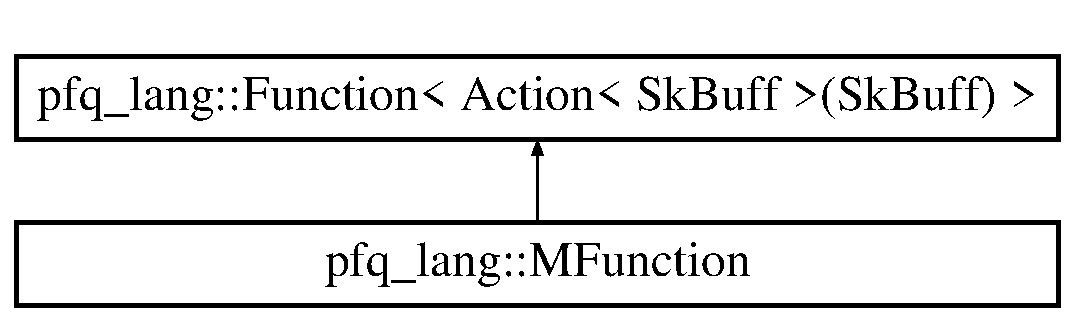
\includegraphics[height=2.000000cm]{structpfq__lang_1_1MFunction}
\end{center}
\end{figure}
\subsection*{Public Member Functions}
\begin{DoxyCompactItemize}
\item 
\hyperlink{structpfq__lang_1_1MFunction_a0903ea045763e5516cbdab8b724ff644}{M\+Function} (std\+::string symbol)
\end{DoxyCompactItemize}
\subsection*{Public Attributes}
\begin{DoxyCompactItemize}
\item 
std\+::string \hyperlink{structpfq__lang_1_1MFunction_af161111a9d2ffbd56bc44ec58a5bbce4}{symbol\+\_\+}
\end{DoxyCompactItemize}
\subsection*{Additional Inherited Members}


\subsection{Constructor \& Destructor Documentation}
\hypertarget{structpfq__lang_1_1MFunction_a0903ea045763e5516cbdab8b724ff644}{\index{pfq\+\_\+lang\+::\+M\+Function@{pfq\+\_\+lang\+::\+M\+Function}!M\+Function@{M\+Function}}
\index{M\+Function@{M\+Function}!pfq\+\_\+lang\+::\+M\+Function@{pfq\+\_\+lang\+::\+M\+Function}}
\subsubsection[{M\+Function}]{\setlength{\rightskip}{0pt plus 5cm}pfq\+\_\+lang\+::\+M\+Function\+::\+M\+Function (
\begin{DoxyParamCaption}
\item[{std\+::string}]{symbol}
\end{DoxyParamCaption}
)\hspace{0.3cm}{\ttfamily [inline]}}}\label{structpfq__lang_1_1MFunction_a0903ea045763e5516cbdab8b724ff644}


\subsection{Member Data Documentation}
\hypertarget{structpfq__lang_1_1MFunction_af161111a9d2ffbd56bc44ec58a5bbce4}{\index{pfq\+\_\+lang\+::\+M\+Function@{pfq\+\_\+lang\+::\+M\+Function}!symbol\+\_\+@{symbol\+\_\+}}
\index{symbol\+\_\+@{symbol\+\_\+}!pfq\+\_\+lang\+::\+M\+Function@{pfq\+\_\+lang\+::\+M\+Function}}
\subsubsection[{symbol\+\_\+}]{\setlength{\rightskip}{0pt plus 5cm}std\+::string pfq\+\_\+lang\+::\+M\+Function\+::symbol\+\_\+}}\label{structpfq__lang_1_1MFunction_af161111a9d2ffbd56bc44ec58a5bbce4}


The documentation for this struct was generated from the following file\+:\begin{DoxyCompactItemize}
\item 
C++/pfq-\/lang/\hyperlink{lang_8hpp}{lang.\+hpp}\end{DoxyCompactItemize}

\hypertarget{structpfq__lang_1_1MFunction1}{\section{pfq\+\_\+lang\+:\+:M\+Function1 Struct Reference}
\label{structpfq__lang_1_1MFunction1}\index{pfq\+\_\+lang\+::\+M\+Function1@{pfq\+\_\+lang\+::\+M\+Function1}}
}


{\ttfamily \#include $<$lang.\+hpp$>$}

Inheritance diagram for pfq\+\_\+lang\+:\+:M\+Function1\+:\begin{figure}[H]
\begin{center}
\leavevmode
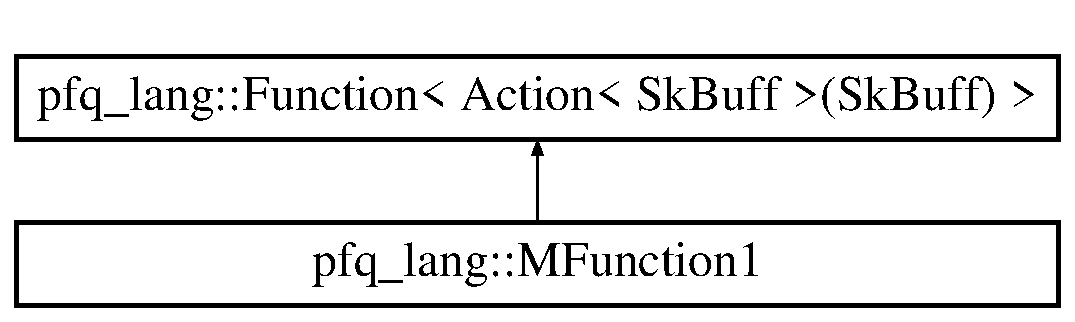
\includegraphics[height=2.000000cm]{structpfq__lang_1_1MFunction1}
\end{center}
\end{figure}
\subsection*{Public Member Functions}
\begin{DoxyCompactItemize}
\item 
{\footnotesize template$<$typename T $>$ }\\\hyperlink{structpfq__lang_1_1MFunction1_aacf9e776abdfd49513ce6bcc6a5315ac}{M\+Function1} (std\+::string symbol, T const \&arg)
\end{DoxyCompactItemize}
\subsection*{Public Attributes}
\begin{DoxyCompactItemize}
\item 
std\+::string \hyperlink{structpfq__lang_1_1MFunction1_a742ffe5f58b94f85b6ddaa8f7c04e02d}{symbol\+\_\+}
\item 
\hyperlink{structpfq__lang_1_1Argument}{Argument} \hyperlink{structpfq__lang_1_1MFunction1_ab6f349bca9961d255f2daf25bc975635}{arg\+\_\+}
\end{DoxyCompactItemize}
\subsection*{Additional Inherited Members}


\subsection{Constructor \& Destructor Documentation}
\hypertarget{structpfq__lang_1_1MFunction1_aacf9e776abdfd49513ce6bcc6a5315ac}{\index{pfq\+\_\+lang\+::\+M\+Function1@{pfq\+\_\+lang\+::\+M\+Function1}!M\+Function1@{M\+Function1}}
\index{M\+Function1@{M\+Function1}!pfq\+\_\+lang\+::\+M\+Function1@{pfq\+\_\+lang\+::\+M\+Function1}}
\subsubsection[{M\+Function1}]{\setlength{\rightskip}{0pt plus 5cm}template$<$typename T $>$ pfq\+\_\+lang\+::\+M\+Function1\+::\+M\+Function1 (
\begin{DoxyParamCaption}
\item[{std\+::string}]{symbol, }
\item[{T const \&}]{arg}
\end{DoxyParamCaption}
)\hspace{0.3cm}{\ttfamily [inline]}}}\label{structpfq__lang_1_1MFunction1_aacf9e776abdfd49513ce6bcc6a5315ac}


\subsection{Member Data Documentation}
\hypertarget{structpfq__lang_1_1MFunction1_ab6f349bca9961d255f2daf25bc975635}{\index{pfq\+\_\+lang\+::\+M\+Function1@{pfq\+\_\+lang\+::\+M\+Function1}!arg\+\_\+@{arg\+\_\+}}
\index{arg\+\_\+@{arg\+\_\+}!pfq\+\_\+lang\+::\+M\+Function1@{pfq\+\_\+lang\+::\+M\+Function1}}
\subsubsection[{arg\+\_\+}]{\setlength{\rightskip}{0pt plus 5cm}{\bf Argument} pfq\+\_\+lang\+::\+M\+Function1\+::arg\+\_\+}}\label{structpfq__lang_1_1MFunction1_ab6f349bca9961d255f2daf25bc975635}
\hypertarget{structpfq__lang_1_1MFunction1_a742ffe5f58b94f85b6ddaa8f7c04e02d}{\index{pfq\+\_\+lang\+::\+M\+Function1@{pfq\+\_\+lang\+::\+M\+Function1}!symbol\+\_\+@{symbol\+\_\+}}
\index{symbol\+\_\+@{symbol\+\_\+}!pfq\+\_\+lang\+::\+M\+Function1@{pfq\+\_\+lang\+::\+M\+Function1}}
\subsubsection[{symbol\+\_\+}]{\setlength{\rightskip}{0pt plus 5cm}std\+::string pfq\+\_\+lang\+::\+M\+Function1\+::symbol\+\_\+}}\label{structpfq__lang_1_1MFunction1_a742ffe5f58b94f85b6ddaa8f7c04e02d}


The documentation for this struct was generated from the following file\+:\begin{DoxyCompactItemize}
\item 
C++/pfq-\/lang/\hyperlink{lang_8hpp}{lang.\+hpp}\end{DoxyCompactItemize}

\hypertarget{structpfq__lang_1_1MFunction2}{\section{pfq\+\_\+lang\+:\+:M\+Function2 Struct Reference}
\label{structpfq__lang_1_1MFunction2}\index{pfq\+\_\+lang\+::\+M\+Function2@{pfq\+\_\+lang\+::\+M\+Function2}}
}


{\ttfamily \#include $<$lang.\+hpp$>$}

Inheritance diagram for pfq\+\_\+lang\+:\+:M\+Function2\+:\begin{figure}[H]
\begin{center}
\leavevmode
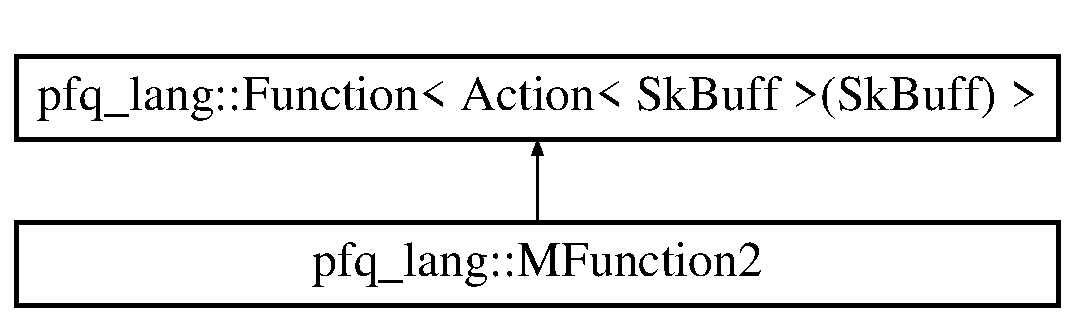
\includegraphics[height=2.000000cm]{structpfq__lang_1_1MFunction2}
\end{center}
\end{figure}
\subsection*{Public Member Functions}
\begin{DoxyCompactItemize}
\item 
\hyperlink{structpfq__lang_1_1MFunction2_aa0ee0ece97ba1a6b58130f374a9c5f3c}{M\+Function2} (std\+::string symbol, std\+::string msg)
\end{DoxyCompactItemize}
\subsection*{Public Attributes}
\begin{DoxyCompactItemize}
\item 
std\+::string \hyperlink{structpfq__lang_1_1MFunction2_a1cf86ea54a5fedb9bfa27fa7866554d0}{symbol\+\_\+}
\item 
\hyperlink{structpfq__lang_1_1Argument}{Argument} \hyperlink{structpfq__lang_1_1MFunction2_a0928b4336ac51e05036af896b479d3b7}{arg\+\_\+}
\end{DoxyCompactItemize}
\subsection*{Additional Inherited Members}


\subsection{Constructor \& Destructor Documentation}
\hypertarget{structpfq__lang_1_1MFunction2_aa0ee0ece97ba1a6b58130f374a9c5f3c}{\index{pfq\+\_\+lang\+::\+M\+Function2@{pfq\+\_\+lang\+::\+M\+Function2}!M\+Function2@{M\+Function2}}
\index{M\+Function2@{M\+Function2}!pfq\+\_\+lang\+::\+M\+Function2@{pfq\+\_\+lang\+::\+M\+Function2}}
\subsubsection[{M\+Function2}]{\setlength{\rightskip}{0pt plus 5cm}pfq\+\_\+lang\+::\+M\+Function2\+::\+M\+Function2 (
\begin{DoxyParamCaption}
\item[{std\+::string}]{symbol, }
\item[{std\+::string}]{msg}
\end{DoxyParamCaption}
)\hspace{0.3cm}{\ttfamily [inline]}}}\label{structpfq__lang_1_1MFunction2_aa0ee0ece97ba1a6b58130f374a9c5f3c}


\subsection{Member Data Documentation}
\hypertarget{structpfq__lang_1_1MFunction2_a0928b4336ac51e05036af896b479d3b7}{\index{pfq\+\_\+lang\+::\+M\+Function2@{pfq\+\_\+lang\+::\+M\+Function2}!arg\+\_\+@{arg\+\_\+}}
\index{arg\+\_\+@{arg\+\_\+}!pfq\+\_\+lang\+::\+M\+Function2@{pfq\+\_\+lang\+::\+M\+Function2}}
\subsubsection[{arg\+\_\+}]{\setlength{\rightskip}{0pt plus 5cm}{\bf Argument} pfq\+\_\+lang\+::\+M\+Function2\+::arg\+\_\+}}\label{structpfq__lang_1_1MFunction2_a0928b4336ac51e05036af896b479d3b7}
\hypertarget{structpfq__lang_1_1MFunction2_a1cf86ea54a5fedb9bfa27fa7866554d0}{\index{pfq\+\_\+lang\+::\+M\+Function2@{pfq\+\_\+lang\+::\+M\+Function2}!symbol\+\_\+@{symbol\+\_\+}}
\index{symbol\+\_\+@{symbol\+\_\+}!pfq\+\_\+lang\+::\+M\+Function2@{pfq\+\_\+lang\+::\+M\+Function2}}
\subsubsection[{symbol\+\_\+}]{\setlength{\rightskip}{0pt plus 5cm}std\+::string pfq\+\_\+lang\+::\+M\+Function2\+::symbol\+\_\+}}\label{structpfq__lang_1_1MFunction2_a1cf86ea54a5fedb9bfa27fa7866554d0}


The documentation for this struct was generated from the following file\+:\begin{DoxyCompactItemize}
\item 
C++/pfq-\/lang/\hyperlink{lang_8hpp}{lang.\+hpp}\end{DoxyCompactItemize}

\hypertarget{structpfq__lang_1_1Predicate}{\section{pfq\+\_\+lang\+:\+:Predicate Struct Reference}
\label{structpfq__lang_1_1Predicate}\index{pfq\+\_\+lang\+::\+Predicate@{pfq\+\_\+lang\+::\+Predicate}}
}


{\ttfamily \#include $<$lang.\+hpp$>$}

Inheritance diagram for pfq\+\_\+lang\+:\+:Predicate\+:\begin{figure}[H]
\begin{center}
\leavevmode
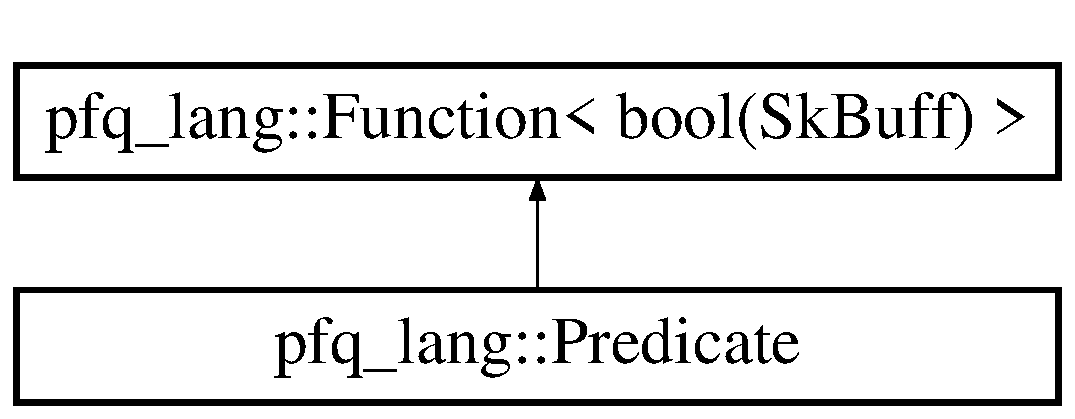
\includegraphics[height=2.000000cm]{structpfq__lang_1_1Predicate}
\end{center}
\end{figure}
\subsection*{Public Member Functions}
\begin{DoxyCompactItemize}
\item 
\hyperlink{structpfq__lang_1_1Predicate_ab91af9569c514d8ec1f8c5c75d74b0c5}{Predicate} (std\+::string symb)
\end{DoxyCompactItemize}
\subsection*{Public Attributes}
\begin{DoxyCompactItemize}
\item 
std\+::string \hyperlink{structpfq__lang_1_1Predicate_a44004d3c8071b374fe4cd1838deb28a3}{symbol\+\_\+}
\end{DoxyCompactItemize}
\subsection*{Additional Inherited Members}


\subsection{Constructor \& Destructor Documentation}
\hypertarget{structpfq__lang_1_1Predicate_ab91af9569c514d8ec1f8c5c75d74b0c5}{\index{pfq\+\_\+lang\+::\+Predicate@{pfq\+\_\+lang\+::\+Predicate}!Predicate@{Predicate}}
\index{Predicate@{Predicate}!pfq\+\_\+lang\+::\+Predicate@{pfq\+\_\+lang\+::\+Predicate}}
\subsubsection[{Predicate}]{\setlength{\rightskip}{0pt plus 5cm}pfq\+\_\+lang\+::\+Predicate\+::\+Predicate (
\begin{DoxyParamCaption}
\item[{std\+::string}]{symb}
\end{DoxyParamCaption}
)\hspace{0.3cm}{\ttfamily [inline]}}}\label{structpfq__lang_1_1Predicate_ab91af9569c514d8ec1f8c5c75d74b0c5}


\subsection{Member Data Documentation}
\hypertarget{structpfq__lang_1_1Predicate_a44004d3c8071b374fe4cd1838deb28a3}{\index{pfq\+\_\+lang\+::\+Predicate@{pfq\+\_\+lang\+::\+Predicate}!symbol\+\_\+@{symbol\+\_\+}}
\index{symbol\+\_\+@{symbol\+\_\+}!pfq\+\_\+lang\+::\+Predicate@{pfq\+\_\+lang\+::\+Predicate}}
\subsubsection[{symbol\+\_\+}]{\setlength{\rightskip}{0pt plus 5cm}std\+::string pfq\+\_\+lang\+::\+Predicate\+::symbol\+\_\+}}\label{structpfq__lang_1_1Predicate_a44004d3c8071b374fe4cd1838deb28a3}


The documentation for this struct was generated from the following file\+:\begin{DoxyCompactItemize}
\item 
C++/pfq-\/lang/\hyperlink{lang_8hpp}{lang.\+hpp}\end{DoxyCompactItemize}

\hypertarget{structpfq__lang_1_1Predicate1}{\section{pfq\+\_\+lang\+:\+:Predicate1 Struct Reference}
\label{structpfq__lang_1_1Predicate1}\index{pfq\+\_\+lang\+::\+Predicate1@{pfq\+\_\+lang\+::\+Predicate1}}
}


{\ttfamily \#include $<$lang.\+hpp$>$}

Inheritance diagram for pfq\+\_\+lang\+:\+:Predicate1\+:\begin{figure}[H]
\begin{center}
\leavevmode
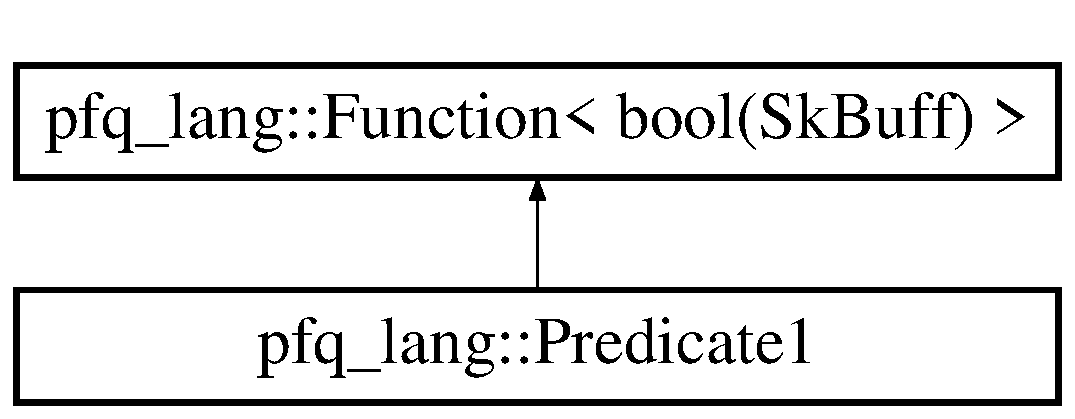
\includegraphics[height=2.000000cm]{structpfq__lang_1_1Predicate1}
\end{center}
\end{figure}
\subsection*{Public Member Functions}
\begin{DoxyCompactItemize}
\item 
{\footnotesize template$<$typename Tp $>$ }\\\hyperlink{structpfq__lang_1_1Predicate1_a18e5c94ef3de56bc383a1163900e8677}{Predicate1} (std\+::string symb, Tp const \&arg)
\end{DoxyCompactItemize}
\subsection*{Public Attributes}
\begin{DoxyCompactItemize}
\item 
std\+::string \hyperlink{structpfq__lang_1_1Predicate1_a1753b4b7aa7045934989a4b24a6fbd36}{symbol\+\_\+}
\item 
\hyperlink{structpfq__lang_1_1Argument}{Argument} \hyperlink{structpfq__lang_1_1Predicate1_a6691bf8b92a93edf9dc77bb6b54b51d5}{arg\+\_\+}
\end{DoxyCompactItemize}
\subsection*{Additional Inherited Members}


\subsection{Constructor \& Destructor Documentation}
\hypertarget{structpfq__lang_1_1Predicate1_a18e5c94ef3de56bc383a1163900e8677}{\index{pfq\+\_\+lang\+::\+Predicate1@{pfq\+\_\+lang\+::\+Predicate1}!Predicate1@{Predicate1}}
\index{Predicate1@{Predicate1}!pfq\+\_\+lang\+::\+Predicate1@{pfq\+\_\+lang\+::\+Predicate1}}
\subsubsection[{Predicate1}]{\setlength{\rightskip}{0pt plus 5cm}template$<$typename Tp $>$ pfq\+\_\+lang\+::\+Predicate1\+::\+Predicate1 (
\begin{DoxyParamCaption}
\item[{std\+::string}]{symb, }
\item[{Tp const \&}]{arg}
\end{DoxyParamCaption}
)\hspace{0.3cm}{\ttfamily [inline]}}}\label{structpfq__lang_1_1Predicate1_a18e5c94ef3de56bc383a1163900e8677}


\subsection{Member Data Documentation}
\hypertarget{structpfq__lang_1_1Predicate1_a6691bf8b92a93edf9dc77bb6b54b51d5}{\index{pfq\+\_\+lang\+::\+Predicate1@{pfq\+\_\+lang\+::\+Predicate1}!arg\+\_\+@{arg\+\_\+}}
\index{arg\+\_\+@{arg\+\_\+}!pfq\+\_\+lang\+::\+Predicate1@{pfq\+\_\+lang\+::\+Predicate1}}
\subsubsection[{arg\+\_\+}]{\setlength{\rightskip}{0pt plus 5cm}{\bf Argument} pfq\+\_\+lang\+::\+Predicate1\+::arg\+\_\+}}\label{structpfq__lang_1_1Predicate1_a6691bf8b92a93edf9dc77bb6b54b51d5}
\hypertarget{structpfq__lang_1_1Predicate1_a1753b4b7aa7045934989a4b24a6fbd36}{\index{pfq\+\_\+lang\+::\+Predicate1@{pfq\+\_\+lang\+::\+Predicate1}!symbol\+\_\+@{symbol\+\_\+}}
\index{symbol\+\_\+@{symbol\+\_\+}!pfq\+\_\+lang\+::\+Predicate1@{pfq\+\_\+lang\+::\+Predicate1}}
\subsubsection[{symbol\+\_\+}]{\setlength{\rightskip}{0pt plus 5cm}std\+::string pfq\+\_\+lang\+::\+Predicate1\+::symbol\+\_\+}}\label{structpfq__lang_1_1Predicate1_a1753b4b7aa7045934989a4b24a6fbd36}


The documentation for this struct was generated from the following file\+:\begin{DoxyCompactItemize}
\item 
C++/pfq-\/lang/\hyperlink{lang_8hpp}{lang.\+hpp}\end{DoxyCompactItemize}

\hypertarget{structpfq__lang_1_1Predicate2}{\section{pfq\+\_\+lang\+:\+:Predicate2$<$ Prop $>$ Struct Template Reference}
\label{structpfq__lang_1_1Predicate2}\index{pfq\+\_\+lang\+::\+Predicate2$<$ Prop $>$@{pfq\+\_\+lang\+::\+Predicate2$<$ Prop $>$}}
}


{\ttfamily \#include $<$lang.\+hpp$>$}

Inheritance diagram for pfq\+\_\+lang\+:\+:Predicate2$<$ Prop $>$\+:\begin{figure}[H]
\begin{center}
\leavevmode
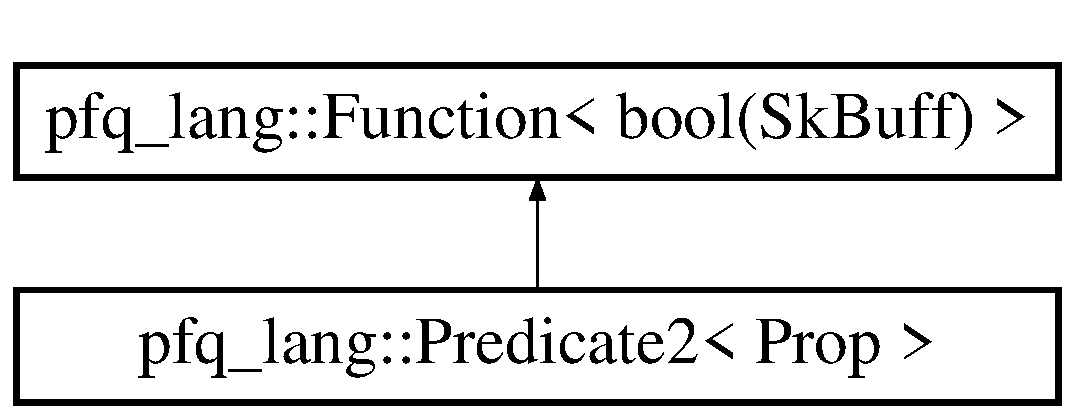
\includegraphics[height=2.000000cm]{structpfq__lang_1_1Predicate2}
\end{center}
\end{figure}
\subsection*{Public Member Functions}
\begin{DoxyCompactItemize}
\item 
\hyperlink{structpfq__lang_1_1Predicate2_a679505645d9410abe961cc4e51aff0c4}{Predicate2} (std\+::string symb, Prop const \&p)
\end{DoxyCompactItemize}
\subsection*{Public Attributes}
\begin{DoxyCompactItemize}
\item 
std\+::string \hyperlink{structpfq__lang_1_1Predicate2_a4e35998af857cdc5da3a515009fb8247}{symbol\+\_\+}
\item 
Prop \hyperlink{structpfq__lang_1_1Predicate2_af3f7dcc4db7db8e2b0dc610b21966224}{prop\+\_\+}
\end{DoxyCompactItemize}
\subsection*{Additional Inherited Members}


\subsection{Constructor \& Destructor Documentation}
\hypertarget{structpfq__lang_1_1Predicate2_a679505645d9410abe961cc4e51aff0c4}{\index{pfq\+\_\+lang\+::\+Predicate2@{pfq\+\_\+lang\+::\+Predicate2}!Predicate2@{Predicate2}}
\index{Predicate2@{Predicate2}!pfq\+\_\+lang\+::\+Predicate2@{pfq\+\_\+lang\+::\+Predicate2}}
\subsubsection[{Predicate2}]{\setlength{\rightskip}{0pt plus 5cm}template$<$typename Prop$>$ {\bf pfq\+\_\+lang\+::\+Predicate2}$<$ Prop $>$\+::{\bf Predicate2} (
\begin{DoxyParamCaption}
\item[{std\+::string}]{symb, }
\item[{Prop const \&}]{p}
\end{DoxyParamCaption}
)\hspace{0.3cm}{\ttfamily [inline]}}}\label{structpfq__lang_1_1Predicate2_a679505645d9410abe961cc4e51aff0c4}


\subsection{Member Data Documentation}
\hypertarget{structpfq__lang_1_1Predicate2_af3f7dcc4db7db8e2b0dc610b21966224}{\index{pfq\+\_\+lang\+::\+Predicate2@{pfq\+\_\+lang\+::\+Predicate2}!prop\+\_\+@{prop\+\_\+}}
\index{prop\+\_\+@{prop\+\_\+}!pfq\+\_\+lang\+::\+Predicate2@{pfq\+\_\+lang\+::\+Predicate2}}
\subsubsection[{prop\+\_\+}]{\setlength{\rightskip}{0pt plus 5cm}template$<$typename Prop$>$ Prop {\bf pfq\+\_\+lang\+::\+Predicate2}$<$ Prop $>$\+::prop\+\_\+}}\label{structpfq__lang_1_1Predicate2_af3f7dcc4db7db8e2b0dc610b21966224}
\hypertarget{structpfq__lang_1_1Predicate2_a4e35998af857cdc5da3a515009fb8247}{\index{pfq\+\_\+lang\+::\+Predicate2@{pfq\+\_\+lang\+::\+Predicate2}!symbol\+\_\+@{symbol\+\_\+}}
\index{symbol\+\_\+@{symbol\+\_\+}!pfq\+\_\+lang\+::\+Predicate2@{pfq\+\_\+lang\+::\+Predicate2}}
\subsubsection[{symbol\+\_\+}]{\setlength{\rightskip}{0pt plus 5cm}template$<$typename Prop$>$ std\+::string {\bf pfq\+\_\+lang\+::\+Predicate2}$<$ Prop $>$\+::symbol\+\_\+}}\label{structpfq__lang_1_1Predicate2_a4e35998af857cdc5da3a515009fb8247}


The documentation for this struct was generated from the following file\+:\begin{DoxyCompactItemize}
\item 
C++/pfq-\/lang/\hyperlink{lang_8hpp}{lang.\+hpp}\end{DoxyCompactItemize}

\hypertarget{structpfq__lang_1_1Predicate3}{\section{pfq\+\_\+lang\+:\+:Predicate3$<$ Prop $>$ Struct Template Reference}
\label{structpfq__lang_1_1Predicate3}\index{pfq\+\_\+lang\+::\+Predicate3$<$ Prop $>$@{pfq\+\_\+lang\+::\+Predicate3$<$ Prop $>$}}
}


{\ttfamily \#include $<$lang.\+hpp$>$}

Inheritance diagram for pfq\+\_\+lang\+:\+:Predicate3$<$ Prop $>$\+:\begin{figure}[H]
\begin{center}
\leavevmode
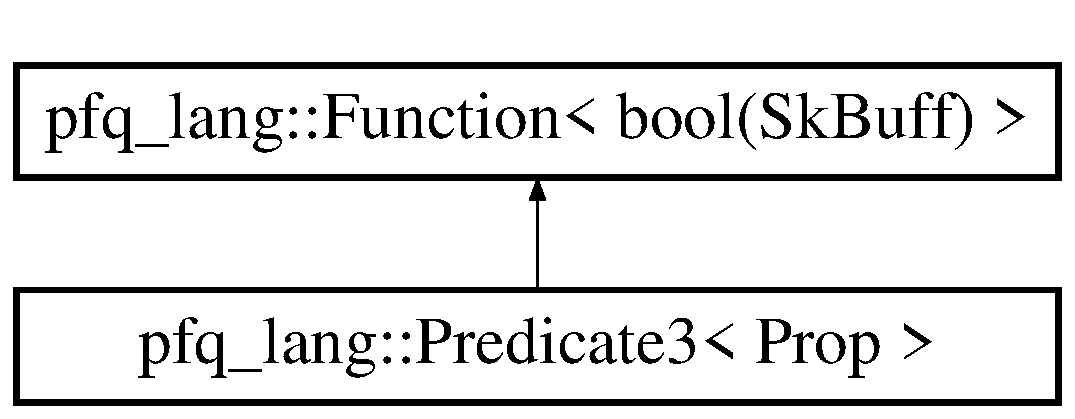
\includegraphics[height=2.000000cm]{structpfq__lang_1_1Predicate3}
\end{center}
\end{figure}
\subsection*{Public Member Functions}
\begin{DoxyCompactItemize}
\item 
{\footnotesize template$<$typename Tp $>$ }\\\hyperlink{structpfq__lang_1_1Predicate3_a1b2f41a793ac559592df47896b2a1180}{Predicate3} (std\+::string symb, Prop const \&p, Tp const \&arg)
\end{DoxyCompactItemize}
\subsection*{Public Attributes}
\begin{DoxyCompactItemize}
\item 
std\+::string \hyperlink{structpfq__lang_1_1Predicate3_acd29e8718600ed723e659fa19251a6f5}{symbol\+\_\+}
\item 
Prop \hyperlink{structpfq__lang_1_1Predicate3_a3d1b5001e401ee228375eefc72da5d88}{prop\+\_\+}
\item 
\hyperlink{structpfq__lang_1_1Argument}{Argument} \hyperlink{structpfq__lang_1_1Predicate3_adf52e42c7be28e2cb25d2f188e501f48}{arg\+\_\+}
\end{DoxyCompactItemize}
\subsection*{Additional Inherited Members}


\subsection{Constructor \& Destructor Documentation}
\hypertarget{structpfq__lang_1_1Predicate3_a1b2f41a793ac559592df47896b2a1180}{\index{pfq\+\_\+lang\+::\+Predicate3@{pfq\+\_\+lang\+::\+Predicate3}!Predicate3@{Predicate3}}
\index{Predicate3@{Predicate3}!pfq\+\_\+lang\+::\+Predicate3@{pfq\+\_\+lang\+::\+Predicate3}}
\subsubsection[{Predicate3}]{\setlength{\rightskip}{0pt plus 5cm}template$<$typename Prop$>$ template$<$typename Tp $>$ {\bf pfq\+\_\+lang\+::\+Predicate3}$<$ Prop $>$\+::{\bf Predicate3} (
\begin{DoxyParamCaption}
\item[{std\+::string}]{symb, }
\item[{Prop const \&}]{p, }
\item[{Tp const \&}]{arg}
\end{DoxyParamCaption}
)\hspace{0.3cm}{\ttfamily [inline]}}}\label{structpfq__lang_1_1Predicate3_a1b2f41a793ac559592df47896b2a1180}


\subsection{Member Data Documentation}
\hypertarget{structpfq__lang_1_1Predicate3_adf52e42c7be28e2cb25d2f188e501f48}{\index{pfq\+\_\+lang\+::\+Predicate3@{pfq\+\_\+lang\+::\+Predicate3}!arg\+\_\+@{arg\+\_\+}}
\index{arg\+\_\+@{arg\+\_\+}!pfq\+\_\+lang\+::\+Predicate3@{pfq\+\_\+lang\+::\+Predicate3}}
\subsubsection[{arg\+\_\+}]{\setlength{\rightskip}{0pt plus 5cm}template$<$typename Prop$>$ {\bf Argument} {\bf pfq\+\_\+lang\+::\+Predicate3}$<$ Prop $>$\+::arg\+\_\+}}\label{structpfq__lang_1_1Predicate3_adf52e42c7be28e2cb25d2f188e501f48}
\hypertarget{structpfq__lang_1_1Predicate3_a3d1b5001e401ee228375eefc72da5d88}{\index{pfq\+\_\+lang\+::\+Predicate3@{pfq\+\_\+lang\+::\+Predicate3}!prop\+\_\+@{prop\+\_\+}}
\index{prop\+\_\+@{prop\+\_\+}!pfq\+\_\+lang\+::\+Predicate3@{pfq\+\_\+lang\+::\+Predicate3}}
\subsubsection[{prop\+\_\+}]{\setlength{\rightskip}{0pt plus 5cm}template$<$typename Prop$>$ Prop {\bf pfq\+\_\+lang\+::\+Predicate3}$<$ Prop $>$\+::prop\+\_\+}}\label{structpfq__lang_1_1Predicate3_a3d1b5001e401ee228375eefc72da5d88}
\hypertarget{structpfq__lang_1_1Predicate3_acd29e8718600ed723e659fa19251a6f5}{\index{pfq\+\_\+lang\+::\+Predicate3@{pfq\+\_\+lang\+::\+Predicate3}!symbol\+\_\+@{symbol\+\_\+}}
\index{symbol\+\_\+@{symbol\+\_\+}!pfq\+\_\+lang\+::\+Predicate3@{pfq\+\_\+lang\+::\+Predicate3}}
\subsubsection[{symbol\+\_\+}]{\setlength{\rightskip}{0pt plus 5cm}template$<$typename Prop$>$ std\+::string {\bf pfq\+\_\+lang\+::\+Predicate3}$<$ Prop $>$\+::symbol\+\_\+}}\label{structpfq__lang_1_1Predicate3_acd29e8718600ed723e659fa19251a6f5}


The documentation for this struct was generated from the following file\+:\begin{DoxyCompactItemize}
\item 
C++/pfq-\/lang/\hyperlink{lang_8hpp}{lang.\+hpp}\end{DoxyCompactItemize}

\hypertarget{structpfq__lang_1_1Property}{\section{pfq\+\_\+lang\+:\+:Property Struct Reference}
\label{structpfq__lang_1_1Property}\index{pfq\+\_\+lang\+::\+Property@{pfq\+\_\+lang\+::\+Property}}
}


{\ttfamily \#include $<$lang.\+hpp$>$}

Inheritance diagram for pfq\+\_\+lang\+:\+:Property\+:\begin{figure}[H]
\begin{center}
\leavevmode
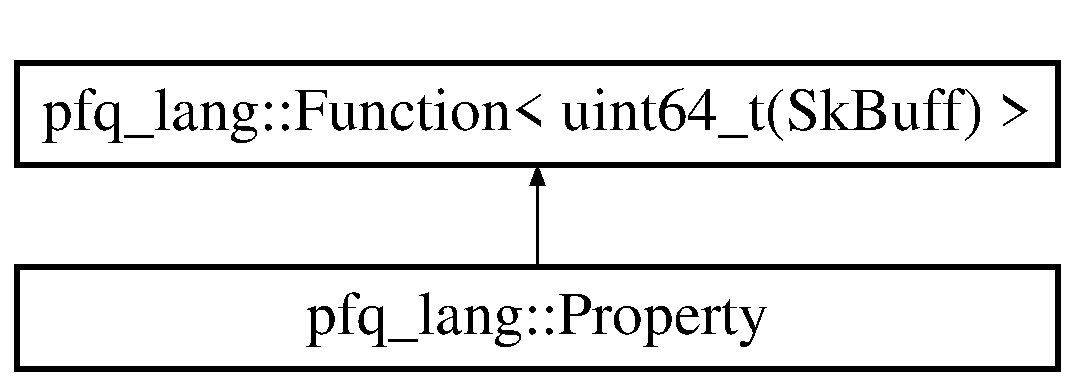
\includegraphics[height=2.000000cm]{structpfq__lang_1_1Property}
\end{center}
\end{figure}
\subsection*{Public Member Functions}
\begin{DoxyCompactItemize}
\item 
\hyperlink{structpfq__lang_1_1Property_a59dc13f20077530b8388cfc7d4e9565b}{Property} (std\+::string symbol)
\end{DoxyCompactItemize}
\subsection*{Public Attributes}
\begin{DoxyCompactItemize}
\item 
std\+::string \hyperlink{structpfq__lang_1_1Property_a60ee4a17e077da3243ded2defb8c4437}{symbol\+\_\+}
\end{DoxyCompactItemize}
\subsection*{Additional Inherited Members}


\subsection{Constructor \& Destructor Documentation}
\hypertarget{structpfq__lang_1_1Property_a59dc13f20077530b8388cfc7d4e9565b}{\index{pfq\+\_\+lang\+::\+Property@{pfq\+\_\+lang\+::\+Property}!Property@{Property}}
\index{Property@{Property}!pfq\+\_\+lang\+::\+Property@{pfq\+\_\+lang\+::\+Property}}
\subsubsection[{Property}]{\setlength{\rightskip}{0pt plus 5cm}pfq\+\_\+lang\+::\+Property\+::\+Property (
\begin{DoxyParamCaption}
\item[{std\+::string}]{symbol}
\end{DoxyParamCaption}
)\hspace{0.3cm}{\ttfamily [inline]}}}\label{structpfq__lang_1_1Property_a59dc13f20077530b8388cfc7d4e9565b}


\subsection{Member Data Documentation}
\hypertarget{structpfq__lang_1_1Property_a60ee4a17e077da3243ded2defb8c4437}{\index{pfq\+\_\+lang\+::\+Property@{pfq\+\_\+lang\+::\+Property}!symbol\+\_\+@{symbol\+\_\+}}
\index{symbol\+\_\+@{symbol\+\_\+}!pfq\+\_\+lang\+::\+Property@{pfq\+\_\+lang\+::\+Property}}
\subsubsection[{symbol\+\_\+}]{\setlength{\rightskip}{0pt plus 5cm}std\+::string pfq\+\_\+lang\+::\+Property\+::symbol\+\_\+}}\label{structpfq__lang_1_1Property_a60ee4a17e077da3243ded2defb8c4437}


The documentation for this struct was generated from the following file\+:\begin{DoxyCompactItemize}
\item 
C++/pfq-\/lang/\hyperlink{lang_8hpp}{lang.\+hpp}\end{DoxyCompactItemize}

\hypertarget{structpfq__lang_1_1Property1}{\section{pfq\+\_\+lang\+:\+:Property1 Struct Reference}
\label{structpfq__lang_1_1Property1}\index{pfq\+\_\+lang\+::\+Property1@{pfq\+\_\+lang\+::\+Property1}}
}


{\ttfamily \#include $<$lang.\+hpp$>$}

\subsection*{Public Member Functions}
\begin{DoxyCompactItemize}
\item 
{\footnotesize template$<$typename T $>$ }\\\hyperlink{structpfq__lang_1_1Property1_ad964f8ae009367e7bbbac06a238eaf25}{Property1} (std\+::string symbol, T const \&arg)
\end{DoxyCompactItemize}
\subsection*{Public Attributes}
\begin{DoxyCompactItemize}
\item 
std\+::string \hyperlink{structpfq__lang_1_1Property1_aa4c4ac30609cd7e17f71dbdf9cf40608}{symbol\+\_\+}
\item 
\hyperlink{structpfq__lang_1_1Argument}{Argument} \hyperlink{structpfq__lang_1_1Property1_a65593e0522f2492c9d77e64dc73cbf9c}{arg\+\_\+}
\end{DoxyCompactItemize}


\subsection{Constructor \& Destructor Documentation}
\hypertarget{structpfq__lang_1_1Property1_ad964f8ae009367e7bbbac06a238eaf25}{\index{pfq\+\_\+lang\+::\+Property1@{pfq\+\_\+lang\+::\+Property1}!Property1@{Property1}}
\index{Property1@{Property1}!pfq\+\_\+lang\+::\+Property1@{pfq\+\_\+lang\+::\+Property1}}
\subsubsection[{Property1}]{\setlength{\rightskip}{0pt plus 5cm}template$<$typename T $>$ pfq\+\_\+lang\+::\+Property1\+::\+Property1 (
\begin{DoxyParamCaption}
\item[{std\+::string}]{symbol, }
\item[{T const \&}]{arg}
\end{DoxyParamCaption}
)\hspace{0.3cm}{\ttfamily [inline]}}}\label{structpfq__lang_1_1Property1_ad964f8ae009367e7bbbac06a238eaf25}


\subsection{Member Data Documentation}
\hypertarget{structpfq__lang_1_1Property1_a65593e0522f2492c9d77e64dc73cbf9c}{\index{pfq\+\_\+lang\+::\+Property1@{pfq\+\_\+lang\+::\+Property1}!arg\+\_\+@{arg\+\_\+}}
\index{arg\+\_\+@{arg\+\_\+}!pfq\+\_\+lang\+::\+Property1@{pfq\+\_\+lang\+::\+Property1}}
\subsubsection[{arg\+\_\+}]{\setlength{\rightskip}{0pt plus 5cm}{\bf Argument} pfq\+\_\+lang\+::\+Property1\+::arg\+\_\+}}\label{structpfq__lang_1_1Property1_a65593e0522f2492c9d77e64dc73cbf9c}
\hypertarget{structpfq__lang_1_1Property1_aa4c4ac30609cd7e17f71dbdf9cf40608}{\index{pfq\+\_\+lang\+::\+Property1@{pfq\+\_\+lang\+::\+Property1}!symbol\+\_\+@{symbol\+\_\+}}
\index{symbol\+\_\+@{symbol\+\_\+}!pfq\+\_\+lang\+::\+Property1@{pfq\+\_\+lang\+::\+Property1}}
\subsubsection[{symbol\+\_\+}]{\setlength{\rightskip}{0pt plus 5cm}std\+::string pfq\+\_\+lang\+::\+Property1\+::symbol\+\_\+}}\label{structpfq__lang_1_1Property1_aa4c4ac30609cd7e17f71dbdf9cf40608}


The documentation for this struct was generated from the following file\+:\begin{DoxyCompactItemize}
\item 
C++/pfq-\/lang/\hyperlink{lang_8hpp}{lang.\+hpp}\end{DoxyCompactItemize}

\hypertarget{structpfq__lang_1_1SkBuff}{\section{pfq\+\_\+lang\+:\+:Sk\+Buff Struct Reference}
\label{structpfq__lang_1_1SkBuff}\index{pfq\+\_\+lang\+::\+Sk\+Buff@{pfq\+\_\+lang\+::\+Sk\+Buff}}
}


{\ttfamily \#include $<$lang.\+hpp$>$}



The documentation for this struct was generated from the following file\+:\begin{DoxyCompactItemize}
\item 
C++/pfq-\/lang/\hyperlink{lang_8hpp}{lang.\+hpp}\end{DoxyCompactItemize}

\hypertarget{structpfq__lang_1_1StorableShow}{\section{pfq\+\_\+lang\+:\+:Storable\+Show$<$ Tp, typename $>$ Struct Template Reference}
\label{structpfq__lang_1_1StorableShow}\index{pfq\+\_\+lang\+::\+Storable\+Show$<$ Tp, typename $>$@{pfq\+\_\+lang\+::\+Storable\+Show$<$ Tp, typename $>$}}
}


{\ttfamily \#include $<$lang.\+hpp$>$}



The documentation for this struct was generated from the following file\+:\begin{DoxyCompactItemize}
\item 
C++/pfq-\/lang/\hyperlink{lang_8hpp}{lang.\+hpp}\end{DoxyCompactItemize}

\hypertarget{structpfq__lang_1_1StorableShow_3_01Tp_00_01typename_01std_1_1enable__if_3_01has__insertion__ope410294f2cbdf117d0cfbbeb13476ebf1}{\section{pfq\+\_\+lang\+:\+:Storable\+Show$<$ Tp, typename std\+:\+:enable\+\_\+if$<$ has\+\_\+insertion\+\_\+operator$<$Tp $>$\+:\+:value $>$\+:\+:type $>$ Struct Template Reference}
\label{structpfq__lang_1_1StorableShow_3_01Tp_00_01typename_01std_1_1enable__if_3_01has__insertion__ope410294f2cbdf117d0cfbbeb13476ebf1}\index{pfq\+\_\+lang\+::\+Storable\+Show$<$ Tp, typename std\+::enable\+\_\+if$<$ has\+\_\+insertion\+\_\+operator$<$\+Tp $>$\+::value $>$\+::type $>$@{pfq\+\_\+lang\+::\+Storable\+Show$<$ Tp, typename std\+::enable\+\_\+if$<$ has\+\_\+insertion\+\_\+operator$<$\+Tp $>$\+::value $>$\+::type $>$}}
}


{\ttfamily \#include $<$lang.\+hpp$>$}

Inheritance diagram for pfq\+\_\+lang\+:\+:Storable\+Show$<$ Tp, typename std\+:\+:enable\+\_\+if$<$ has\+\_\+insertion\+\_\+operator$<$Tp $>$\+:\+:value $>$\+:\+:type $>$\+:\begin{figure}[H]
\begin{center}
\leavevmode
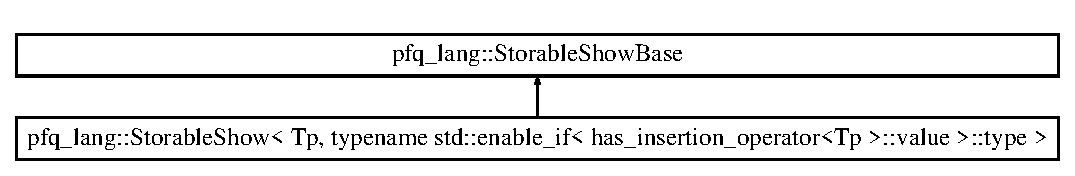
\includegraphics[height=1.911263cm]{structpfq__lang_1_1StorableShow_3_01Tp_00_01typename_01std_1_1enable__if_3_01has__insertion__ope410294f2cbdf117d0cfbbeb13476ebf1}
\end{center}
\end{figure}
\subsection*{Public Member Functions}
\begin{DoxyCompactItemize}
\item 
\hyperlink{structpfq__lang_1_1StorableShow_3_01Tp_00_01typename_01std_1_1enable__if_3_01has__insertion__ope410294f2cbdf117d0cfbbeb13476ebf1_a3d453254c884983343eb2c4e65a78345}{Storable\+Show} (Tp v)
\item 
const void $\ast$ \hyperlink{structpfq__lang_1_1StorableShow_3_01Tp_00_01typename_01std_1_1enable__if_3_01has__insertion__ope410294f2cbdf117d0cfbbeb13476ebf1_a5ec739ac33a3f48073bae2d30bb05630}{forall\+\_\+addr} () const override
\item 
std\+::string \hyperlink{structpfq__lang_1_1StorableShow_3_01Tp_00_01typename_01std_1_1enable__if_3_01has__insertion__ope410294f2cbdf117d0cfbbeb13476ebf1_a3125673ba8d8ca64063815f62b039da5}{forall\+\_\+show} () const override
\end{DoxyCompactItemize}
\subsection*{Public Attributes}
\begin{DoxyCompactItemize}
\item 
Tp \hyperlink{structpfq__lang_1_1StorableShow_3_01Tp_00_01typename_01std_1_1enable__if_3_01has__insertion__ope410294f2cbdf117d0cfbbeb13476ebf1_a2d991395164d152da6dd32aa6f795984}{value}
\end{DoxyCompactItemize}
\subsection*{Additional Inherited Members}


\subsection{Constructor \& Destructor Documentation}
\hypertarget{structpfq__lang_1_1StorableShow_3_01Tp_00_01typename_01std_1_1enable__if_3_01has__insertion__ope410294f2cbdf117d0cfbbeb13476ebf1_a3d453254c884983343eb2c4e65a78345}{\index{pfq\+\_\+lang\+::\+Storable\+Show$<$ Tp, typename std\+::enable\+\_\+if$<$ has\+\_\+insertion\+\_\+operator$<$\+Tp $>$\+::value $>$\+::type $>$@{pfq\+\_\+lang\+::\+Storable\+Show$<$ Tp, typename std\+::enable\+\_\+if$<$ has\+\_\+insertion\+\_\+operator$<$\+Tp $>$\+::value $>$\+::type $>$}!Storable\+Show@{Storable\+Show}}
\index{Storable\+Show@{Storable\+Show}!pfq\+\_\+lang\+::\+Storable\+Show$<$ Tp, typename std\+::enable\+\_\+if$<$ has\+\_\+insertion\+\_\+operator$<$\+Tp $>$\+::value $>$\+::type $>$@{pfq\+\_\+lang\+::\+Storable\+Show$<$ Tp, typename std\+::enable\+\_\+if$<$ has\+\_\+insertion\+\_\+operator$<$\+Tp $>$\+::value $>$\+::type $>$}}
\subsubsection[{Storable\+Show}]{\setlength{\rightskip}{0pt plus 5cm}template$<$typename Tp $>$ {\bf pfq\+\_\+lang\+::\+Storable\+Show}$<$ Tp, typename std\+::enable\+\_\+if$<$ {\bf has\+\_\+insertion\+\_\+operator}$<$Tp $>$\+::{\bf value} $>$\+::type $>$\+::{\bf Storable\+Show} (
\begin{DoxyParamCaption}
\item[{Tp}]{v}
\end{DoxyParamCaption}
)\hspace{0.3cm}{\ttfamily [inline]}}}\label{structpfq__lang_1_1StorableShow_3_01Tp_00_01typename_01std_1_1enable__if_3_01has__insertion__ope410294f2cbdf117d0cfbbeb13476ebf1_a3d453254c884983343eb2c4e65a78345}


\subsection{Member Function Documentation}
\hypertarget{structpfq__lang_1_1StorableShow_3_01Tp_00_01typename_01std_1_1enable__if_3_01has__insertion__ope410294f2cbdf117d0cfbbeb13476ebf1_a5ec739ac33a3f48073bae2d30bb05630}{\index{pfq\+\_\+lang\+::\+Storable\+Show$<$ Tp, typename std\+::enable\+\_\+if$<$ has\+\_\+insertion\+\_\+operator$<$\+Tp $>$\+::value $>$\+::type $>$@{pfq\+\_\+lang\+::\+Storable\+Show$<$ Tp, typename std\+::enable\+\_\+if$<$ has\+\_\+insertion\+\_\+operator$<$\+Tp $>$\+::value $>$\+::type $>$}!forall\+\_\+addr@{forall\+\_\+addr}}
\index{forall\+\_\+addr@{forall\+\_\+addr}!pfq\+\_\+lang\+::\+Storable\+Show$<$ Tp, typename std\+::enable\+\_\+if$<$ has\+\_\+insertion\+\_\+operator$<$\+Tp $>$\+::value $>$\+::type $>$@{pfq\+\_\+lang\+::\+Storable\+Show$<$ Tp, typename std\+::enable\+\_\+if$<$ has\+\_\+insertion\+\_\+operator$<$\+Tp $>$\+::value $>$\+::type $>$}}
\subsubsection[{forall\+\_\+addr}]{\setlength{\rightskip}{0pt plus 5cm}template$<$typename Tp $>$ const void$\ast$ {\bf pfq\+\_\+lang\+::\+Storable\+Show}$<$ Tp, typename std\+::enable\+\_\+if$<$ {\bf has\+\_\+insertion\+\_\+operator}$<$Tp $>$\+::{\bf value} $>$\+::type $>$\+::forall\+\_\+addr (
\begin{DoxyParamCaption}
{}
\end{DoxyParamCaption}
) const\hspace{0.3cm}{\ttfamily [inline]}, {\ttfamily [override]}, {\ttfamily [virtual]}}}\label{structpfq__lang_1_1StorableShow_3_01Tp_00_01typename_01std_1_1enable__if_3_01has__insertion__ope410294f2cbdf117d0cfbbeb13476ebf1_a5ec739ac33a3f48073bae2d30bb05630}


Implements \hyperlink{structpfq__lang_1_1StorableShowBase_a7ad3bcb5b59da3fb0f1a82ce1b284afd}{pfq\+\_\+lang\+::\+Storable\+Show\+Base}.

\hypertarget{structpfq__lang_1_1StorableShow_3_01Tp_00_01typename_01std_1_1enable__if_3_01has__insertion__ope410294f2cbdf117d0cfbbeb13476ebf1_a3125673ba8d8ca64063815f62b039da5}{\index{pfq\+\_\+lang\+::\+Storable\+Show$<$ Tp, typename std\+::enable\+\_\+if$<$ has\+\_\+insertion\+\_\+operator$<$\+Tp $>$\+::value $>$\+::type $>$@{pfq\+\_\+lang\+::\+Storable\+Show$<$ Tp, typename std\+::enable\+\_\+if$<$ has\+\_\+insertion\+\_\+operator$<$\+Tp $>$\+::value $>$\+::type $>$}!forall\+\_\+show@{forall\+\_\+show}}
\index{forall\+\_\+show@{forall\+\_\+show}!pfq\+\_\+lang\+::\+Storable\+Show$<$ Tp, typename std\+::enable\+\_\+if$<$ has\+\_\+insertion\+\_\+operator$<$\+Tp $>$\+::value $>$\+::type $>$@{pfq\+\_\+lang\+::\+Storable\+Show$<$ Tp, typename std\+::enable\+\_\+if$<$ has\+\_\+insertion\+\_\+operator$<$\+Tp $>$\+::value $>$\+::type $>$}}
\subsubsection[{forall\+\_\+show}]{\setlength{\rightskip}{0pt plus 5cm}template$<$typename Tp $>$ std\+::string {\bf pfq\+\_\+lang\+::\+Storable\+Show}$<$ Tp, typename std\+::enable\+\_\+if$<$ {\bf has\+\_\+insertion\+\_\+operator}$<$Tp $>$\+::{\bf value} $>$\+::type $>$\+::forall\+\_\+show (
\begin{DoxyParamCaption}
{}
\end{DoxyParamCaption}
) const\hspace{0.3cm}{\ttfamily [inline]}, {\ttfamily [override]}, {\ttfamily [virtual]}}}\label{structpfq__lang_1_1StorableShow_3_01Tp_00_01typename_01std_1_1enable__if_3_01has__insertion__ope410294f2cbdf117d0cfbbeb13476ebf1_a3125673ba8d8ca64063815f62b039da5}


Implements \hyperlink{structpfq__lang_1_1StorableShowBase_aea533aa9bd20171aae76157c9ebbd43e}{pfq\+\_\+lang\+::\+Storable\+Show\+Base}.



\subsection{Member Data Documentation}
\hypertarget{structpfq__lang_1_1StorableShow_3_01Tp_00_01typename_01std_1_1enable__if_3_01has__insertion__ope410294f2cbdf117d0cfbbeb13476ebf1_a2d991395164d152da6dd32aa6f795984}{\index{pfq\+\_\+lang\+::\+Storable\+Show$<$ Tp, typename std\+::enable\+\_\+if$<$ has\+\_\+insertion\+\_\+operator$<$\+Tp $>$\+::value $>$\+::type $>$@{pfq\+\_\+lang\+::\+Storable\+Show$<$ Tp, typename std\+::enable\+\_\+if$<$ has\+\_\+insertion\+\_\+operator$<$\+Tp $>$\+::value $>$\+::type $>$}!value@{value}}
\index{value@{value}!pfq\+\_\+lang\+::\+Storable\+Show$<$ Tp, typename std\+::enable\+\_\+if$<$ has\+\_\+insertion\+\_\+operator$<$\+Tp $>$\+::value $>$\+::type $>$@{pfq\+\_\+lang\+::\+Storable\+Show$<$ Tp, typename std\+::enable\+\_\+if$<$ has\+\_\+insertion\+\_\+operator$<$\+Tp $>$\+::value $>$\+::type $>$}}
\subsubsection[{value}]{\setlength{\rightskip}{0pt plus 5cm}template$<$typename Tp $>$ Tp {\bf pfq\+\_\+lang\+::\+Storable\+Show}$<$ Tp, typename std\+::enable\+\_\+if$<$ {\bf has\+\_\+insertion\+\_\+operator}$<$Tp $>$\+::value $>$\+::type $>$\+::value}}\label{structpfq__lang_1_1StorableShow_3_01Tp_00_01typename_01std_1_1enable__if_3_01has__insertion__ope410294f2cbdf117d0cfbbeb13476ebf1_a2d991395164d152da6dd32aa6f795984}


The documentation for this struct was generated from the following file\+:\begin{DoxyCompactItemize}
\item 
C++/pfq-\/lang/\hyperlink{lang_8hpp}{lang.\+hpp}\end{DoxyCompactItemize}

\hypertarget{structpfq__lang_1_1StorableShow_3_01Tp_00_01typename_01std_1_1enable__if_3_9has__insertion__operc98e9de6b381c730d9d28da7df10d016}{\section{pfq\+\_\+lang\+:\+:Storable\+Show$<$ Tp, typename std\+:\+:enable\+\_\+if$<$!has\+\_\+insertion\+\_\+operator$<$Tp $>$\+:\+:value $>$\+:\+:type $>$ Struct Template Reference}
\label{structpfq__lang_1_1StorableShow_3_01Tp_00_01typename_01std_1_1enable__if_3_9has__insertion__operc98e9de6b381c730d9d28da7df10d016}\index{pfq\+\_\+lang\+::\+Storable\+Show$<$ Tp, typename std\+::enable\+\_\+if$<$"!has\+\_\+insertion\+\_\+operator$<$\+Tp $>$\+::value $>$\+::type $>$@{pfq\+\_\+lang\+::\+Storable\+Show$<$ Tp, typename std\+::enable\+\_\+if$<$"!has\+\_\+insertion\+\_\+operator$<$\+Tp $>$\+::value $>$\+::type $>$}}
}


{\ttfamily \#include $<$lang.\+hpp$>$}

Inheritance diagram for pfq\+\_\+lang\+:\+:Storable\+Show$<$ Tp, typename std\+:\+:enable\+\_\+if$<$!has\+\_\+insertion\+\_\+operator$<$Tp $>$\+:\+:value $>$\+:\+:type $>$\+:\begin{figure}[H]
\begin{center}
\leavevmode
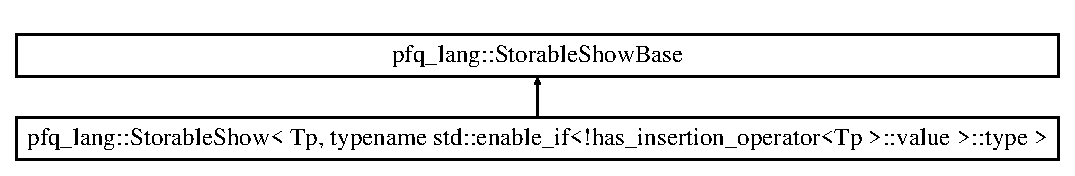
\includegraphics[height=1.917808cm]{structpfq__lang_1_1StorableShow_3_01Tp_00_01typename_01std_1_1enable__if_3_9has__insertion__operc98e9de6b381c730d9d28da7df10d016}
\end{center}
\end{figure}
\subsection*{Public Member Functions}
\begin{DoxyCompactItemize}
\item 
\hyperlink{structpfq__lang_1_1StorableShow_3_01Tp_00_01typename_01std_1_1enable__if_3_9has__insertion__operc98e9de6b381c730d9d28da7df10d016_aa1c419e6174b34eec53430c6f2a479a2}{Storable\+Show} (Tp v)
\item 
const void $\ast$ \hyperlink{structpfq__lang_1_1StorableShow_3_01Tp_00_01typename_01std_1_1enable__if_3_9has__insertion__operc98e9de6b381c730d9d28da7df10d016_a1d2ff6a788af963ba952a4d83dac48c7}{forall\+\_\+addr} () const override
\item 
std\+::string \hyperlink{structpfq__lang_1_1StorableShow_3_01Tp_00_01typename_01std_1_1enable__if_3_9has__insertion__operc98e9de6b381c730d9d28da7df10d016_aba784c55c209b0c780bc9deca4e698e8}{forall\+\_\+show} () const override
\end{DoxyCompactItemize}
\subsection*{Public Attributes}
\begin{DoxyCompactItemize}
\item 
Tp \hyperlink{structpfq__lang_1_1StorableShow_3_01Tp_00_01typename_01std_1_1enable__if_3_9has__insertion__operc98e9de6b381c730d9d28da7df10d016_a98fec55c620c3c3d998c2b75fc63fa23}{value}
\end{DoxyCompactItemize}
\subsection*{Additional Inherited Members}


\subsection{Constructor \& Destructor Documentation}
\hypertarget{structpfq__lang_1_1StorableShow_3_01Tp_00_01typename_01std_1_1enable__if_3_9has__insertion__operc98e9de6b381c730d9d28da7df10d016_aa1c419e6174b34eec53430c6f2a479a2}{\index{pfq\+\_\+lang\+::\+Storable\+Show$<$ Tp, typename std\+::enable\+\_\+if$<$"!has\+\_\+insertion\+\_\+operator$<$\+Tp $>$\+::value $>$\+::type $>$@{pfq\+\_\+lang\+::\+Storable\+Show$<$ Tp, typename std\+::enable\+\_\+if$<$"!has\+\_\+insertion\+\_\+operator$<$\+Tp $>$\+::value $>$\+::type $>$}!Storable\+Show@{Storable\+Show}}
\index{Storable\+Show@{Storable\+Show}!pfq\+\_\+lang\+::\+Storable\+Show$<$ Tp, typename std\+::enable\+\_\+if$<$"!has\+\_\+insertion\+\_\+operator$<$\+Tp $>$\+::value $>$\+::type $>$@{pfq\+\_\+lang\+::\+Storable\+Show$<$ Tp, typename std\+::enable\+\_\+if$<$"!has\+\_\+insertion\+\_\+operator$<$\+Tp $>$\+::value $>$\+::type $>$}}
\subsubsection[{Storable\+Show}]{\setlength{\rightskip}{0pt plus 5cm}template$<$typename Tp $>$ {\bf pfq\+\_\+lang\+::\+Storable\+Show}$<$ Tp, typename std\+::enable\+\_\+if$<$!{\bf has\+\_\+insertion\+\_\+operator}$<$Tp $>$\+::{\bf value} $>$\+::type $>$\+::{\bf Storable\+Show} (
\begin{DoxyParamCaption}
\item[{Tp}]{v}
\end{DoxyParamCaption}
)\hspace{0.3cm}{\ttfamily [inline]}}}\label{structpfq__lang_1_1StorableShow_3_01Tp_00_01typename_01std_1_1enable__if_3_9has__insertion__operc98e9de6b381c730d9d28da7df10d016_aa1c419e6174b34eec53430c6f2a479a2}


\subsection{Member Function Documentation}
\hypertarget{structpfq__lang_1_1StorableShow_3_01Tp_00_01typename_01std_1_1enable__if_3_9has__insertion__operc98e9de6b381c730d9d28da7df10d016_a1d2ff6a788af963ba952a4d83dac48c7}{\index{pfq\+\_\+lang\+::\+Storable\+Show$<$ Tp, typename std\+::enable\+\_\+if$<$"!has\+\_\+insertion\+\_\+operator$<$\+Tp $>$\+::value $>$\+::type $>$@{pfq\+\_\+lang\+::\+Storable\+Show$<$ Tp, typename std\+::enable\+\_\+if$<$"!has\+\_\+insertion\+\_\+operator$<$\+Tp $>$\+::value $>$\+::type $>$}!forall\+\_\+addr@{forall\+\_\+addr}}
\index{forall\+\_\+addr@{forall\+\_\+addr}!pfq\+\_\+lang\+::\+Storable\+Show$<$ Tp, typename std\+::enable\+\_\+if$<$"!has\+\_\+insertion\+\_\+operator$<$\+Tp $>$\+::value $>$\+::type $>$@{pfq\+\_\+lang\+::\+Storable\+Show$<$ Tp, typename std\+::enable\+\_\+if$<$"!has\+\_\+insertion\+\_\+operator$<$\+Tp $>$\+::value $>$\+::type $>$}}
\subsubsection[{forall\+\_\+addr}]{\setlength{\rightskip}{0pt plus 5cm}template$<$typename Tp $>$ const void$\ast$ {\bf pfq\+\_\+lang\+::\+Storable\+Show}$<$ Tp, typename std\+::enable\+\_\+if$<$!{\bf has\+\_\+insertion\+\_\+operator}$<$Tp $>$\+::{\bf value} $>$\+::type $>$\+::forall\+\_\+addr (
\begin{DoxyParamCaption}
{}
\end{DoxyParamCaption}
) const\hspace{0.3cm}{\ttfamily [inline]}, {\ttfamily [override]}, {\ttfamily [virtual]}}}\label{structpfq__lang_1_1StorableShow_3_01Tp_00_01typename_01std_1_1enable__if_3_9has__insertion__operc98e9de6b381c730d9d28da7df10d016_a1d2ff6a788af963ba952a4d83dac48c7}


Implements \hyperlink{structpfq__lang_1_1StorableShowBase_a7ad3bcb5b59da3fb0f1a82ce1b284afd}{pfq\+\_\+lang\+::\+Storable\+Show\+Base}.

\hypertarget{structpfq__lang_1_1StorableShow_3_01Tp_00_01typename_01std_1_1enable__if_3_9has__insertion__operc98e9de6b381c730d9d28da7df10d016_aba784c55c209b0c780bc9deca4e698e8}{\index{pfq\+\_\+lang\+::\+Storable\+Show$<$ Tp, typename std\+::enable\+\_\+if$<$"!has\+\_\+insertion\+\_\+operator$<$\+Tp $>$\+::value $>$\+::type $>$@{pfq\+\_\+lang\+::\+Storable\+Show$<$ Tp, typename std\+::enable\+\_\+if$<$"!has\+\_\+insertion\+\_\+operator$<$\+Tp $>$\+::value $>$\+::type $>$}!forall\+\_\+show@{forall\+\_\+show}}
\index{forall\+\_\+show@{forall\+\_\+show}!pfq\+\_\+lang\+::\+Storable\+Show$<$ Tp, typename std\+::enable\+\_\+if$<$"!has\+\_\+insertion\+\_\+operator$<$\+Tp $>$\+::value $>$\+::type $>$@{pfq\+\_\+lang\+::\+Storable\+Show$<$ Tp, typename std\+::enable\+\_\+if$<$"!has\+\_\+insertion\+\_\+operator$<$\+Tp $>$\+::value $>$\+::type $>$}}
\subsubsection[{forall\+\_\+show}]{\setlength{\rightskip}{0pt plus 5cm}template$<$typename Tp $>$ std\+::string {\bf pfq\+\_\+lang\+::\+Storable\+Show}$<$ Tp, typename std\+::enable\+\_\+if$<$!{\bf has\+\_\+insertion\+\_\+operator}$<$Tp $>$\+::{\bf value} $>$\+::type $>$\+::forall\+\_\+show (
\begin{DoxyParamCaption}
{}
\end{DoxyParamCaption}
) const\hspace{0.3cm}{\ttfamily [inline]}, {\ttfamily [override]}, {\ttfamily [virtual]}}}\label{structpfq__lang_1_1StorableShow_3_01Tp_00_01typename_01std_1_1enable__if_3_9has__insertion__operc98e9de6b381c730d9d28da7df10d016_aba784c55c209b0c780bc9deca4e698e8}


Implements \hyperlink{structpfq__lang_1_1StorableShowBase_aea533aa9bd20171aae76157c9ebbd43e}{pfq\+\_\+lang\+::\+Storable\+Show\+Base}.



\subsection{Member Data Documentation}
\hypertarget{structpfq__lang_1_1StorableShow_3_01Tp_00_01typename_01std_1_1enable__if_3_9has__insertion__operc98e9de6b381c730d9d28da7df10d016_a98fec55c620c3c3d998c2b75fc63fa23}{\index{pfq\+\_\+lang\+::\+Storable\+Show$<$ Tp, typename std\+::enable\+\_\+if$<$"!has\+\_\+insertion\+\_\+operator$<$\+Tp $>$\+::value $>$\+::type $>$@{pfq\+\_\+lang\+::\+Storable\+Show$<$ Tp, typename std\+::enable\+\_\+if$<$"!has\+\_\+insertion\+\_\+operator$<$\+Tp $>$\+::value $>$\+::type $>$}!value@{value}}
\index{value@{value}!pfq\+\_\+lang\+::\+Storable\+Show$<$ Tp, typename std\+::enable\+\_\+if$<$"!has\+\_\+insertion\+\_\+operator$<$\+Tp $>$\+::value $>$\+::type $>$@{pfq\+\_\+lang\+::\+Storable\+Show$<$ Tp, typename std\+::enable\+\_\+if$<$"!has\+\_\+insertion\+\_\+operator$<$\+Tp $>$\+::value $>$\+::type $>$}}
\subsubsection[{value}]{\setlength{\rightskip}{0pt plus 5cm}template$<$typename Tp $>$ Tp {\bf pfq\+\_\+lang\+::\+Storable\+Show}$<$ Tp, typename std\+::enable\+\_\+if$<$!{\bf has\+\_\+insertion\+\_\+operator}$<$Tp $>$\+::value $>$\+::type $>$\+::value}}\label{structpfq__lang_1_1StorableShow_3_01Tp_00_01typename_01std_1_1enable__if_3_9has__insertion__operc98e9de6b381c730d9d28da7df10d016_a98fec55c620c3c3d998c2b75fc63fa23}


The documentation for this struct was generated from the following file\+:\begin{DoxyCompactItemize}
\item 
C++/pfq-\/lang/\hyperlink{lang_8hpp}{lang.\+hpp}\end{DoxyCompactItemize}

\hypertarget{structpfq__lang_1_1StorableShowBase}{\section{pfq\+\_\+lang\+:\+:Storable\+Show\+Base Struct Reference}
\label{structpfq__lang_1_1StorableShowBase}\index{pfq\+\_\+lang\+::\+Storable\+Show\+Base@{pfq\+\_\+lang\+::\+Storable\+Show\+Base}}
}


{\ttfamily \#include $<$lang.\+hpp$>$}

Inheritance diagram for pfq\+\_\+lang\+:\+:Storable\+Show\+Base\+:\begin{figure}[H]
\begin{center}
\leavevmode
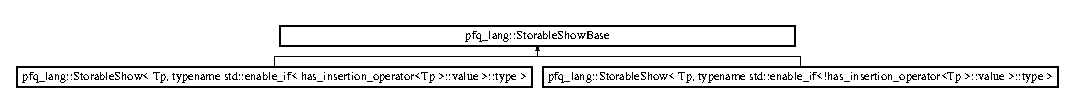
\includegraphics[height=0.955631cm]{structpfq__lang_1_1StorableShowBase}
\end{center}
\end{figure}
\subsection*{Public Member Functions}
\begin{DoxyCompactItemize}
\item 
virtual std\+::string \hyperlink{structpfq__lang_1_1StorableShowBase_aea533aa9bd20171aae76157c9ebbd43e}{forall\+\_\+show} () const =0
\item 
virtual void const $\ast$ \hyperlink{structpfq__lang_1_1StorableShowBase_a7ad3bcb5b59da3fb0f1a82ce1b284afd}{forall\+\_\+addr} () const =0
\end{DoxyCompactItemize}
\subsection*{Static Public Member Functions}
\begin{DoxyCompactItemize}
\item 
static const void $\ast$ \hyperlink{structpfq__lang_1_1StorableShowBase_a964df7b0275fbbf16c6ad55c139f4810}{get\+\_\+addr} (std\+::string const \&that)
\item 
{\footnotesize template$<$typename T $>$ }\\static const void $\ast$ \hyperlink{structpfq__lang_1_1StorableShowBase_a27a48e4b29ec89bb550d4a42613dcb3e}{get\+\_\+addr} (T const \&that)
\end{DoxyCompactItemize}


\subsection{Member Function Documentation}
\hypertarget{structpfq__lang_1_1StorableShowBase_a7ad3bcb5b59da3fb0f1a82ce1b284afd}{\index{pfq\+\_\+lang\+::\+Storable\+Show\+Base@{pfq\+\_\+lang\+::\+Storable\+Show\+Base}!forall\+\_\+addr@{forall\+\_\+addr}}
\index{forall\+\_\+addr@{forall\+\_\+addr}!pfq\+\_\+lang\+::\+Storable\+Show\+Base@{pfq\+\_\+lang\+::\+Storable\+Show\+Base}}
\subsubsection[{forall\+\_\+addr}]{\setlength{\rightskip}{0pt plus 5cm}virtual void const$\ast$ pfq\+\_\+lang\+::\+Storable\+Show\+Base\+::forall\+\_\+addr (
\begin{DoxyParamCaption}
{}
\end{DoxyParamCaption}
) const\hspace{0.3cm}{\ttfamily [pure virtual]}}}\label{structpfq__lang_1_1StorableShowBase_a7ad3bcb5b59da3fb0f1a82ce1b284afd}


Implemented in \hyperlink{structpfq__lang_1_1StorableShow_3_01Tp_00_01typename_01std_1_1enable__if_3_9has__insertion__operc98e9de6b381c730d9d28da7df10d016_a1d2ff6a788af963ba952a4d83dac48c7}{pfq\+\_\+lang\+::\+Storable\+Show$<$ Tp, typename std\+::enable\+\_\+if$<$!has\+\_\+insertion\+\_\+operator$<$\+Tp $>$\+::value $>$\+::type $>$}, and \hyperlink{structpfq__lang_1_1StorableShow_3_01Tp_00_01typename_01std_1_1enable__if_3_01has__insertion__ope410294f2cbdf117d0cfbbeb13476ebf1_a5ec739ac33a3f48073bae2d30bb05630}{pfq\+\_\+lang\+::\+Storable\+Show$<$ Tp, typename std\+::enable\+\_\+if$<$ has\+\_\+insertion\+\_\+operator$<$\+Tp $>$\+::value $>$\+::type $>$}.

\hypertarget{structpfq__lang_1_1StorableShowBase_aea533aa9bd20171aae76157c9ebbd43e}{\index{pfq\+\_\+lang\+::\+Storable\+Show\+Base@{pfq\+\_\+lang\+::\+Storable\+Show\+Base}!forall\+\_\+show@{forall\+\_\+show}}
\index{forall\+\_\+show@{forall\+\_\+show}!pfq\+\_\+lang\+::\+Storable\+Show\+Base@{pfq\+\_\+lang\+::\+Storable\+Show\+Base}}
\subsubsection[{forall\+\_\+show}]{\setlength{\rightskip}{0pt plus 5cm}virtual std\+::string pfq\+\_\+lang\+::\+Storable\+Show\+Base\+::forall\+\_\+show (
\begin{DoxyParamCaption}
{}
\end{DoxyParamCaption}
) const\hspace{0.3cm}{\ttfamily [pure virtual]}}}\label{structpfq__lang_1_1StorableShowBase_aea533aa9bd20171aae76157c9ebbd43e}


Implemented in \hyperlink{structpfq__lang_1_1StorableShow_3_01Tp_00_01typename_01std_1_1enable__if_3_9has__insertion__operc98e9de6b381c730d9d28da7df10d016_aba784c55c209b0c780bc9deca4e698e8}{pfq\+\_\+lang\+::\+Storable\+Show$<$ Tp, typename std\+::enable\+\_\+if$<$!has\+\_\+insertion\+\_\+operator$<$\+Tp $>$\+::value $>$\+::type $>$}, and \hyperlink{structpfq__lang_1_1StorableShow_3_01Tp_00_01typename_01std_1_1enable__if_3_01has__insertion__ope410294f2cbdf117d0cfbbeb13476ebf1_a3125673ba8d8ca64063815f62b039da5}{pfq\+\_\+lang\+::\+Storable\+Show$<$ Tp, typename std\+::enable\+\_\+if$<$ has\+\_\+insertion\+\_\+operator$<$\+Tp $>$\+::value $>$\+::type $>$}.

\hypertarget{structpfq__lang_1_1StorableShowBase_a964df7b0275fbbf16c6ad55c139f4810}{\index{pfq\+\_\+lang\+::\+Storable\+Show\+Base@{pfq\+\_\+lang\+::\+Storable\+Show\+Base}!get\+\_\+addr@{get\+\_\+addr}}
\index{get\+\_\+addr@{get\+\_\+addr}!pfq\+\_\+lang\+::\+Storable\+Show\+Base@{pfq\+\_\+lang\+::\+Storable\+Show\+Base}}
\subsubsection[{get\+\_\+addr}]{\setlength{\rightskip}{0pt plus 5cm}static const void$\ast$ pfq\+\_\+lang\+::\+Storable\+Show\+Base\+::get\+\_\+addr (
\begin{DoxyParamCaption}
\item[{std\+::string const \&}]{that}
\end{DoxyParamCaption}
)\hspace{0.3cm}{\ttfamily [inline]}, {\ttfamily [static]}}}\label{structpfq__lang_1_1StorableShowBase_a964df7b0275fbbf16c6ad55c139f4810}
\hypertarget{structpfq__lang_1_1StorableShowBase_a27a48e4b29ec89bb550d4a42613dcb3e}{\index{pfq\+\_\+lang\+::\+Storable\+Show\+Base@{pfq\+\_\+lang\+::\+Storable\+Show\+Base}!get\+\_\+addr@{get\+\_\+addr}}
\index{get\+\_\+addr@{get\+\_\+addr}!pfq\+\_\+lang\+::\+Storable\+Show\+Base@{pfq\+\_\+lang\+::\+Storable\+Show\+Base}}
\subsubsection[{get\+\_\+addr}]{\setlength{\rightskip}{0pt plus 5cm}template$<$typename T $>$ static const void$\ast$ pfq\+\_\+lang\+::\+Storable\+Show\+Base\+::get\+\_\+addr (
\begin{DoxyParamCaption}
\item[{T const \&}]{that}
\end{DoxyParamCaption}
)\hspace{0.3cm}{\ttfamily [inline]}, {\ttfamily [static]}}}\label{structpfq__lang_1_1StorableShowBase_a27a48e4b29ec89bb550d4a42613dcb3e}


The documentation for this struct was generated from the following file\+:\begin{DoxyCompactItemize}
\item 
C++/pfq-\/lang/\hyperlink{lang_8hpp}{lang.\+hpp}\end{DoxyCompactItemize}

\chapter{File Documentation}
\hypertarget{default_8hpp}{\section{C++/pfq-\/lang/default.hpp File Reference}
\label{default_8hpp}\index{C++/pfq-\/lang/default.\+hpp@{C++/pfq-\/lang/default.\+hpp}}
}
{\ttfamily \#include $<$pfq-\/lang/lang.\+hpp$>$}\\*
{\ttfamily \#include $<$pfq-\/lang/details.\+hpp$>$}\\*
{\ttfamily \#include $<$functional$>$}\\*
{\ttfamily \#include $<$arpa/inet.\+h$>$}\\*
\subsection*{Namespaces}
\begin{DoxyCompactItemize}
\item 
 \hyperlink{namespacepfq__lang}{pfq\+\_\+lang}
\item 
 \hyperlink{namespacepfq__lang_1_1anonymous__namespace_02default_8hpp_03}{pfq\+\_\+lang\+::anonymous\+\_\+namespace\{default.\+hpp\}}
\end{DoxyCompactItemize}
\subsection*{Functions}
\begin{DoxyCompactItemize}
\item 
{\footnotesize template$<$typename P1 , typename P2 $>$ }\\auto \hyperlink{namespacepfq__lang_aa6f7aa80466e4cfd61a341fcf7a2eda4}{pfq\+\_\+lang\+::operator\&} (P1 const \&p1, P2 const \&p2) -\/$>$ decltype(predicate2(combinator(nullptr), p1, p2))
\item 
{\footnotesize template$<$typename P1 , typename P2 $>$ }\\auto \hyperlink{namespacepfq__lang_adeec773d44aae2b2f2957e1498c4ce8f}{pfq\+\_\+lang\+::operator$\vert$} (P1 const \&p1, P2 const \&p2) -\/$>$ decltype(predicate2(combinator(nullptr), p1, p2))
\item 
{\footnotesize template$<$typename P1 , typename P2 $>$ }\\auto \hyperlink{namespacepfq__lang_a29166c6bb957d6edd6892b7081f574df}{pfq\+\_\+lang\+::operator$^\wedge$} (P1 const \&p1, P2 const \&p2) -\/$>$ decltype(predicate2(combinator(nullptr), p1, p2))
\item 
{\footnotesize template$<$typename P $>$ }\\auto \hyperlink{namespacepfq__lang_a222bd443a88e69ec2b3acd886bb80e37}{pfq\+\_\+lang\+::operator$<$} (P const \&prop, uint64\+\_\+t arg) -\/$>$ decltype(predicate4(nullptr, prop, arg))
\item 
{\footnotesize template$<$typename P $>$ }\\auto \hyperlink{namespacepfq__lang_a67b8e80010c51a199869c1c2368b87be}{pfq\+\_\+lang\+::operator$<$=} (P const \&prop, uint64\+\_\+t arg) -\/$>$ decltype(predicate4(nullptr, prop, arg))
\item 
{\footnotesize template$<$typename P $>$ }\\auto \hyperlink{namespacepfq__lang_ab210ad49979608b563eaa74a0d42b63a}{pfq\+\_\+lang\+::operator$>$} (P const \&prop, uint64\+\_\+t arg) -\/$>$ decltype(predicate4(nullptr, prop, arg))
\item 
{\footnotesize template$<$typename P $>$ }\\auto \hyperlink{namespacepfq__lang_ac37c4aac9486ceca12814ccd9b4c3306}{pfq\+\_\+lang\+::operator$>$=} (P const \&prop, uint64\+\_\+t arg) -\/$>$ decltype(predicate4(nullptr, prop, arg))
\item 
{\footnotesize template$<$typename P $>$ }\\auto \hyperlink{namespacepfq__lang_ac55d12423490f127fcb57b29535ca791}{pfq\+\_\+lang\+::operator==} (P const \&prop, uint64\+\_\+t arg) -\/$>$ decltype(predicate4(nullptr, prop, arg))
\item 
{\footnotesize template$<$typename P $>$ }\\auto \hyperlink{namespacepfq__lang_a982f7b6137536d7e75fe9b2c13d581d4}{pfq\+\_\+lang\+::operator!=} (P const \&prop, uint64\+\_\+t arg) -\/$>$ decltype(predicate4(nullptr, prop, arg))
\item 
{\footnotesize template$<$typename P $>$ }\\auto \hyperlink{namespacepfq__lang_a9e93958b1fecbd660154947b474ffd05}{pfq\+\_\+lang\+::any\+\_\+bit} (P const \&prop, uint64\+\_\+t mask) -\/$>$ decltype(predicate4(nullptr, prop, mask))
\item 
{\footnotesize template$<$typename P $>$ }\\auto \hyperlink{namespacepfq__lang_a424b5bd6563ed52fd84807def8ba2f5f}{pfq\+\_\+lang\+::all\+\_\+bit} (P const \&prop, uint64\+\_\+t mask) -\/$>$ decltype(predicate4(nullptr, prop, mask))
\end{DoxyCompactItemize}
\subsection*{Variables}
\begin{DoxyCompactItemize}
\item 
auto \hyperlink{namespacepfq__lang_1_1anonymous__namespace_02default_8hpp_03_a43ee18537268245a58354e044a134df5}{pfq\+\_\+lang\+::anonymous\+\_\+namespace\{default.\+hpp\}\+::is\+\_\+ip} = predicate (\char`\"{}is\+\_\+ip\char`\"{})
\item 
auto \hyperlink{namespacepfq__lang_1_1anonymous__namespace_02default_8hpp_03_a107437a3539c86e92035db62e88b7d81}{pfq\+\_\+lang\+::anonymous\+\_\+namespace\{default.\+hpp\}\+::is\+\_\+ip6} = predicate (\char`\"{}is\+\_\+ip6\char`\"{})
\item 
auto \hyperlink{namespacepfq__lang_1_1anonymous__namespace_02default_8hpp_03_a120b37089690955fc25203beb98f0fe7}{pfq\+\_\+lang\+::anonymous\+\_\+namespace\{default.\+hpp\}\+::is\+\_\+udp} = predicate (\char`\"{}is\+\_\+udp\char`\"{})
\item 
auto \hyperlink{namespacepfq__lang_1_1anonymous__namespace_02default_8hpp_03_a219c50fd572a25336a32e00cf527c565}{pfq\+\_\+lang\+::anonymous\+\_\+namespace\{default.\+hpp\}\+::is\+\_\+tcp} = predicate (\char`\"{}is\+\_\+tcp\char`\"{})
\item 
auto \hyperlink{namespacepfq__lang_1_1anonymous__namespace_02default_8hpp_03_aecfdadd54cbd2d4e93a7f246b6bcd0fc}{pfq\+\_\+lang\+::anonymous\+\_\+namespace\{default.\+hpp\}\+::is\+\_\+icmp} = predicate (\char`\"{}is\+\_\+icmp\char`\"{})
\item 
auto \hyperlink{namespacepfq__lang_1_1anonymous__namespace_02default_8hpp_03_a31e93829d19f72f4aece81f57d7cef9c}{pfq\+\_\+lang\+::anonymous\+\_\+namespace\{default.\+hpp\}\+::is\+\_\+udp6} = predicate (\char`\"{}is\+\_\+udp6\char`\"{})
\item 
auto \hyperlink{namespacepfq__lang_1_1anonymous__namespace_02default_8hpp_03_a096d3a0faa81e83be5cfeb025526275d}{pfq\+\_\+lang\+::anonymous\+\_\+namespace\{default.\+hpp\}\+::is\+\_\+tcp6} = predicate (\char`\"{}is\+\_\+tcp6\char`\"{})
\item 
auto \hyperlink{namespacepfq__lang_1_1anonymous__namespace_02default_8hpp_03_abbce0d21ac217034eac2cd1366f78695}{pfq\+\_\+lang\+::anonymous\+\_\+namespace\{default.\+hpp\}\+::is\+\_\+icmp6} = predicate (\char`\"{}is\+\_\+icmp6\char`\"{})
\item 
auto \hyperlink{namespacepfq__lang_1_1anonymous__namespace_02default_8hpp_03_aa447a7b5765c5c5f9036de8358f86434}{pfq\+\_\+lang\+::anonymous\+\_\+namespace\{default.\+hpp\}\+::is\+\_\+l3\+\_\+proto} = \mbox{[}$\,$\mbox{]} (uint16\+\_\+t type) \{ return predicate1 (\char`\"{}is\+\_\+l3\+\_\+proto\char`\"{}, type); \}
\item 
auto \hyperlink{namespacepfq__lang_1_1anonymous__namespace_02default_8hpp_03_ac2363f68f819b20eb7afc4acdcdd0bf0}{pfq\+\_\+lang\+::anonymous\+\_\+namespace\{default.\+hpp\}\+::is\+\_\+l4\+\_\+proto} = \mbox{[}$\,$\mbox{]} (uint8\+\_\+t proto) \{ return predicate1 (\char`\"{}is\+\_\+l4\+\_\+proto\char`\"{}, proto); \}
\item 
auto \hyperlink{namespacepfq__lang_1_1anonymous__namespace_02default_8hpp_03_ad2840696177c5f4f6f2072bcaae7407e}{pfq\+\_\+lang\+::anonymous\+\_\+namespace\{default.\+hpp\}\+::has\+\_\+port} = \mbox{[}$\,$\mbox{]} (uint16\+\_\+t port) \{ return predicate1 (\char`\"{}is\+\_\+port\char`\"{}, port); \}
\item 
auto \hyperlink{namespacepfq__lang_1_1anonymous__namespace_02default_8hpp_03_ad6d8ed8e08a448b3bf5d23a929d887f9}{pfq\+\_\+lang\+::anonymous\+\_\+namespace\{default.\+hpp\}\+::has\+\_\+src\+\_\+port} = \mbox{[}$\,$\mbox{]} (uint16\+\_\+t port) \{ return predicate1 (\char`\"{}is\+\_\+src\+\_\+port\char`\"{}, port); \}
\item 
auto \hyperlink{namespacepfq__lang_1_1anonymous__namespace_02default_8hpp_03_accc3aed36db0c762dd6c95f3706c8741}{pfq\+\_\+lang\+::anonymous\+\_\+namespace\{default.\+hpp\}\+::has\+\_\+dst\+\_\+port} = \mbox{[}$\,$\mbox{]} (uint16\+\_\+t port) \{ return predicate1 (\char`\"{}is\+\_\+dst\+\_\+port\char`\"{}, port); \}
\item 
auto \hyperlink{namespacepfq__lang_1_1anonymous__namespace_02default_8hpp_03_ac3ef3eefe441b183db012637b4459836}{pfq\+\_\+lang\+::anonymous\+\_\+namespace\{default.\+hpp\}\+::has\+\_\+addr}
\item 
auto \hyperlink{namespacepfq__lang_1_1anonymous__namespace_02default_8hpp_03_aabc75799de679df702f4179ead82114c}{pfq\+\_\+lang\+::anonymous\+\_\+namespace\{default.\+hpp\}\+::has\+\_\+src\+\_\+addr}
\item 
auto \hyperlink{namespacepfq__lang_1_1anonymous__namespace_02default_8hpp_03_af223a0513ceffa69c0b8535a7cca12da}{pfq\+\_\+lang\+::anonymous\+\_\+namespace\{default.\+hpp\}\+::has\+\_\+dst\+\_\+addr}
\item 
auto \hyperlink{namespacepfq__lang_1_1anonymous__namespace_02default_8hpp_03_a32aab6804e2daac2458f7c050ed69cf1}{pfq\+\_\+lang\+::anonymous\+\_\+namespace\{default.\+hpp\}\+::is\+\_\+flow} = predicate (\char`\"{}is\+\_\+flow\char`\"{})
\item 
auto \hyperlink{namespacepfq__lang_1_1anonymous__namespace_02default_8hpp_03_a30a0c8d9bcd28cd17c6c1699c3339c3f}{pfq\+\_\+lang\+::anonymous\+\_\+namespace\{default.\+hpp\}\+::has\+\_\+vlan} = predicate (\char`\"{}has\+\_\+vlan\char`\"{})
\item 
auto \hyperlink{namespacepfq__lang_1_1anonymous__namespace_02default_8hpp_03_adddd2dea56164719f2853af158911a80}{pfq\+\_\+lang\+::anonymous\+\_\+namespace\{default.\+hpp\}\+::has\+\_\+vid} = \mbox{[}$\,$\mbox{]} (int value) \{ return predicate1 (\char`\"{}has\+\_\+vid\char`\"{}, value); \}
\item 
auto \hyperlink{namespacepfq__lang_1_1anonymous__namespace_02default_8hpp_03_a0f9dc3f39bf9793e766b6312718483f1}{pfq\+\_\+lang\+::anonymous\+\_\+namespace\{default.\+hpp\}\+::has\+\_\+mark} = \mbox{[}$\,$\mbox{]} (unsigned long value) \{ return predicate1(\char`\"{}has\+\_\+mark\char`\"{}, value); \}
\item 
auto \hyperlink{namespacepfq__lang_1_1anonymous__namespace_02default_8hpp_03_afc29e9877341008196788bba2bde3e04}{pfq\+\_\+lang\+::anonymous\+\_\+namespace\{default.\+hpp\}\+::ip\+\_\+tos} = property(\char`\"{}ip\+\_\+tos\char`\"{})
\item 
auto \hyperlink{namespacepfq__lang_1_1anonymous__namespace_02default_8hpp_03_a172d424ed5943dda09a80d7c63be9490}{pfq\+\_\+lang\+::anonymous\+\_\+namespace\{default.\+hpp\}\+::ip\+\_\+tot\+\_\+len} = property(\char`\"{}ip\+\_\+tot\+\_\+len\char`\"{})
\item 
auto \hyperlink{namespacepfq__lang_1_1anonymous__namespace_02default_8hpp_03_a7e1fd2e2131451ca8afe2f8ab07b97a8}{pfq\+\_\+lang\+::anonymous\+\_\+namespace\{default.\+hpp\}\+::ip\+\_\+id} = property(\char`\"{}ip\+\_\+id\char`\"{})
\item 
auto \hyperlink{namespacepfq__lang_1_1anonymous__namespace_02default_8hpp_03_a29f207a5d209c3968f5d2e8f3c19c239}{pfq\+\_\+lang\+::anonymous\+\_\+namespace\{default.\+hpp\}\+::ip\+\_\+frag} = property(\char`\"{}ip\+\_\+frag\char`\"{})
\item 
auto \hyperlink{namespacepfq__lang_1_1anonymous__namespace_02default_8hpp_03_a3fb042ff6cf76a1f01b4e97e35b30507}{pfq\+\_\+lang\+::anonymous\+\_\+namespace\{default.\+hpp\}\+::ip\+\_\+ttl} = property(\char`\"{}ip\+\_\+ttl\char`\"{})
\item 
auto \hyperlink{namespacepfq__lang_1_1anonymous__namespace_02default_8hpp_03_a4b3ea94407fb5f52e5dfd9e2511f04a8}{pfq\+\_\+lang\+::anonymous\+\_\+namespace\{default.\+hpp\}\+::tcp\+\_\+source} = property(\char`\"{}tcp\+\_\+source\char`\"{})
\item 
auto \hyperlink{namespacepfq__lang_1_1anonymous__namespace_02default_8hpp_03_a3123415d88452c599055bf8eaba2211e}{pfq\+\_\+lang\+::anonymous\+\_\+namespace\{default.\+hpp\}\+::tcp\+\_\+dest} = property(\char`\"{}tcp\+\_\+dest\char`\"{})
\item 
auto \hyperlink{namespacepfq__lang_1_1anonymous__namespace_02default_8hpp_03_aa8e6b2154ad12220fd1f348c37eaa621}{pfq\+\_\+lang\+::anonymous\+\_\+namespace\{default.\+hpp\}\+::tcp\+\_\+hdrlen} = property(\char`\"{}tcp\+\_\+hdrlen\char`\"{})
\item 
auto \hyperlink{namespacepfq__lang_1_1anonymous__namespace_02default_8hpp_03_a7d2943522cfb795fcb82c894dba83292}{pfq\+\_\+lang\+::anonymous\+\_\+namespace\{default.\+hpp\}\+::udp\+\_\+source} = property(\char`\"{}udp\+\_\+source\char`\"{})
\item 
auto \hyperlink{namespacepfq__lang_1_1anonymous__namespace_02default_8hpp_03_a4f869214bea58f5ed42b3faded5ab088}{pfq\+\_\+lang\+::anonymous\+\_\+namespace\{default.\+hpp\}\+::udp\+\_\+dest} = property(\char`\"{}udp\+\_\+dest\char`\"{})
\item 
auto \hyperlink{namespacepfq__lang_1_1anonymous__namespace_02default_8hpp_03_ab0dcf23db0f218100e7fe51562e0add1}{pfq\+\_\+lang\+::anonymous\+\_\+namespace\{default.\+hpp\}\+::udp\+\_\+len} = property(\char`\"{}udp\+\_\+len\char`\"{})
\item 
auto \hyperlink{namespacepfq__lang_1_1anonymous__namespace_02default_8hpp_03_a4adff7ced08caa2d0016a911dae6d2ed}{pfq\+\_\+lang\+::anonymous\+\_\+namespace\{default.\+hpp\}\+::icmp\+\_\+type} = property(\char`\"{}icmp\+\_\+type\char`\"{})
\item 
auto \hyperlink{namespacepfq__lang_1_1anonymous__namespace_02default_8hpp_03_aad0f666aca065f5aaf283857e5c933ce}{pfq\+\_\+lang\+::anonymous\+\_\+namespace\{default.\+hpp\}\+::icmp\+\_\+code} = property(\char`\"{}icmp\+\_\+code\char`\"{})
\item 
auto \hyperlink{namespacepfq__lang_1_1anonymous__namespace_02default_8hpp_03_af339132b49ec24313a1b3d33cefb1628}{pfq\+\_\+lang\+::anonymous\+\_\+namespace\{default.\+hpp\}\+::steer\+\_\+link} = netfunction(\char`\"{}steer\+\_\+link\char`\"{})
\item 
auto \hyperlink{namespacepfq__lang_1_1anonymous__namespace_02default_8hpp_03_ad32804252244d5b572b9f5fe0cdda675}{pfq\+\_\+lang\+::anonymous\+\_\+namespace\{default.\+hpp\}\+::steer\+\_\+vlan} = netfunction(\char`\"{}steer\+\_\+vlan\char`\"{})
\item 
auto \hyperlink{namespacepfq__lang_1_1anonymous__namespace_02default_8hpp_03_ab44cbea49db522460c5bce82d04280cd}{pfq\+\_\+lang\+::anonymous\+\_\+namespace\{default.\+hpp\}\+::steer\+\_\+ip} = netfunction(\char`\"{}steer\+\_\+ip\char`\"{})
\item 
auto \hyperlink{namespacepfq__lang_1_1anonymous__namespace_02default_8hpp_03_a011de504f63578469615a302f823d238}{pfq\+\_\+lang\+::anonymous\+\_\+namespace\{default.\+hpp\}\+::steer\+\_\+ip6} = netfunction(\char`\"{}steer\+\_\+ip6\char`\"{})
\item 
auto \hyperlink{namespacepfq__lang_1_1anonymous__namespace_02default_8hpp_03_aee7b4eb8c316f9c0cd6ee7bc22b517ef}{pfq\+\_\+lang\+::anonymous\+\_\+namespace\{default.\+hpp\}\+::steer\+\_\+flow} = netfunction(\char`\"{}steer\+\_\+flow\char`\"{})
\item 
auto \hyperlink{namespacepfq__lang_1_1anonymous__namespace_02default_8hpp_03_a16b18fdc10f8dd8c0974d9f0d6c13af9}{pfq\+\_\+lang\+::anonymous\+\_\+namespace\{default.\+hpp\}\+::steer\+\_\+rtp} = netfunction(\char`\"{}steer\+\_\+rtp\char`\"{})
\item 
auto \hyperlink{namespacepfq__lang_1_1anonymous__namespace_02default_8hpp_03_a2c53e95204f3841919f780940b607d68}{pfq\+\_\+lang\+::anonymous\+\_\+namespace\{default.\+hpp\}\+::steer\+\_\+net}
\item 
auto \hyperlink{namespacepfq__lang_1_1anonymous__namespace_02default_8hpp_03_a27d30e7744c84a7cdc41a710ee16b885}{pfq\+\_\+lang\+::anonymous\+\_\+namespace\{default.\+hpp\}\+::ip} = netfunction(\char`\"{}ip\char`\"{})
\item 
auto \hyperlink{namespacepfq__lang_1_1anonymous__namespace_02default_8hpp_03_a566cbe8627dd2ae05071690ef64dbd12}{pfq\+\_\+lang\+::anonymous\+\_\+namespace\{default.\+hpp\}\+::ip6} = netfunction(\char`\"{}ip6\char`\"{})
\item 
auto \hyperlink{namespacepfq__lang_1_1anonymous__namespace_02default_8hpp_03_a1f18de2040dd9d74a07b1c535911abdf}{pfq\+\_\+lang\+::anonymous\+\_\+namespace\{default.\+hpp\}\+::udp} = netfunction(\char`\"{}udp\char`\"{})
\item 
auto \hyperlink{namespacepfq__lang_1_1anonymous__namespace_02default_8hpp_03_a4046140746c0012b4d1ea8d3ef53f084}{pfq\+\_\+lang\+::anonymous\+\_\+namespace\{default.\+hpp\}\+::tcp} = netfunction(\char`\"{}tcp\char`\"{})
\item 
auto \hyperlink{namespacepfq__lang_1_1anonymous__namespace_02default_8hpp_03_a84b7a888d00d5dfea606f7df96ba0ad3}{pfq\+\_\+lang\+::anonymous\+\_\+namespace\{default.\+hpp\}\+::udp6} = netfunction(\char`\"{}udp6\char`\"{})
\item 
auto \hyperlink{namespacepfq__lang_1_1anonymous__namespace_02default_8hpp_03_a734af11014e5ccaef77d6fa39cea0d6b}{pfq\+\_\+lang\+::anonymous\+\_\+namespace\{default.\+hpp\}\+::tcp6} = netfunction(\char`\"{}tcp6\char`\"{})
\item 
auto \hyperlink{namespacepfq__lang_1_1anonymous__namespace_02default_8hpp_03_ab1e01b177ae34e48f61eed78580aeac0}{pfq\+\_\+lang\+::anonymous\+\_\+namespace\{default.\+hpp\}\+::icmp6} = netfunction(\char`\"{}icmp6\char`\"{})
\item 
auto \hyperlink{namespacepfq__lang_1_1anonymous__namespace_02default_8hpp_03_a78f5b5ec52d0563083f1e41d746843f6}{pfq\+\_\+lang\+::anonymous\+\_\+namespace\{default.\+hpp\}\+::vlan} = netfunction(\char`\"{}vlan\char`\"{})
\item 
auto \hyperlink{namespacepfq__lang_1_1anonymous__namespace_02default_8hpp_03_a180c8185595965a528fd2590da7dbeb9}{pfq\+\_\+lang\+::anonymous\+\_\+namespace\{default.\+hpp\}\+::icmp} = netfunction(\char`\"{}icmp\char`\"{})
\item 
auto \hyperlink{namespacepfq__lang_1_1anonymous__namespace_02default_8hpp_03_a90497b962aed613834286418cd7ea722}{pfq\+\_\+lang\+::anonymous\+\_\+namespace\{default.\+hpp\}\+::flow} = netfunction(\char`\"{}flow\char`\"{})
\item 
auto \hyperlink{namespacepfq__lang_1_1anonymous__namespace_02default_8hpp_03_a13ac072f4d7f860256ef22d7f5a1a9ac}{pfq\+\_\+lang\+::anonymous\+\_\+namespace\{default.\+hpp\}\+::rtp} = netfunction(\char`\"{}rtp\char`\"{})
\item 
auto \hyperlink{namespacepfq__lang_1_1anonymous__namespace_02default_8hpp_03_a3b7dd001dfb2302c93212313c0bfa82a}{pfq\+\_\+lang\+::anonymous\+\_\+namespace\{default.\+hpp\}\+::broadcast} = netfunction(\char`\"{}broadcast\char`\"{})
\item 
auto \hyperlink{namespacepfq__lang_1_1anonymous__namespace_02default_8hpp_03_a68a2502f951a2b671a7d0496609f5d2a}{pfq\+\_\+lang\+::anonymous\+\_\+namespace\{default.\+hpp\}\+::kernel} = netfunction(\char`\"{}kernel\char`\"{})
\item 
auto \hyperlink{namespacepfq__lang_1_1anonymous__namespace_02default_8hpp_03_a453450a8ebf5660ab590a3ffb79057e1}{pfq\+\_\+lang\+::anonymous\+\_\+namespace\{default.\+hpp\}\+::forward\+\_\+kernel} = netfunction(\char`\"{}forward\+\_\+kernel\char`\"{})
\item 
auto \hyperlink{namespacepfq__lang_1_1anonymous__namespace_02default_8hpp_03_ad708862e729d0cc6a217d86bb25b1061}{pfq\+\_\+lang\+::anonymous\+\_\+namespace\{default.\+hpp\}\+::sink} = netfunction(\char`\"{}sink\char`\"{})
\item 
auto \hyperlink{namespacepfq__lang_1_1anonymous__namespace_02default_8hpp_03_abed0412f2864624f755594077d255b1e}{pfq\+\_\+lang\+::anonymous\+\_\+namespace\{default.\+hpp\}\+::drop} = netfunction(\char`\"{}drop\char`\"{})
\item 
auto \hyperlink{namespacepfq__lang_1_1anonymous__namespace_02default_8hpp_03_ae78caafebdc64f9180032a049b7c3b3a}{pfq\+\_\+lang\+::anonymous\+\_\+namespace\{default.\+hpp\}\+::unit} = netfunction(\char`\"{}unit\char`\"{})
\item 
auto \hyperlink{namespacepfq__lang_1_1anonymous__namespace_02default_8hpp_03_a27a683ef93570a66844e1a0106e6336a}{pfq\+\_\+lang\+::anonymous\+\_\+namespace\{default.\+hpp\}\+::class\+\_\+} = \mbox{[}$\,$\mbox{]} (int value) \{ return netfunction1(\char`\"{}class\char`\"{}, value); \}
\item 
auto \hyperlink{namespacepfq__lang_1_1anonymous__namespace_02default_8hpp_03_a9baf04657b3da63a2a6d574bbcdafb76}{pfq\+\_\+lang\+::anonymous\+\_\+namespace\{default.\+hpp\}\+::deliver} = \mbox{[}$\,$\mbox{]} (int value) \{ return netfunction1(\char`\"{}deliver\char`\"{}, value); \}
\item 
auto \hyperlink{namespacepfq__lang_1_1anonymous__namespace_02default_8hpp_03_a7fbe4b2614dd240727bf1696b4d06523}{pfq\+\_\+lang\+::anonymous\+\_\+namespace\{default.\+hpp\}\+::forward} = \mbox{[}$\,$\mbox{]} (int index) \{ return netfunction1(\char`\"{}forward\char`\"{}, index); \}
\item 
auto \hyperlink{namespacepfq__lang_1_1anonymous__namespace_02default_8hpp_03_ad6142fe3a0fc859f25ea16956f52a5f0}{pfq\+\_\+lang\+::anonymous\+\_\+namespace\{default.\+hpp\}\+::mark} = \mbox{[}$\,$\mbox{]} (unsigned long value) \{ return netfunction1(\char`\"{}mark\char`\"{}, value); \}
\item 
auto \hyperlink{namespacepfq__lang_1_1anonymous__namespace_02default_8hpp_03_a876b4be1c6cf97e317f74242d8fb3da4}{pfq\+\_\+lang\+::anonymous\+\_\+namespace\{default.\+hpp\}\+::dummy} = \mbox{[}$\,$\mbox{]} (int value) \{ return netfunction1(\char`\"{}dummy\char`\"{}, value); \}
\item 
auto \hyperlink{namespacepfq__lang_1_1anonymous__namespace_02default_8hpp_03_a14246183085ec07f08ab9b0d53907ae5}{pfq\+\_\+lang\+::anonymous\+\_\+namespace\{default.\+hpp\}\+::inc} = \mbox{[}$\,$\mbox{]} (int value) \{ return netfunction1(\char`\"{}inc\char`\"{}, value); \}
\item 
auto \hyperlink{namespacepfq__lang_1_1anonymous__namespace_02default_8hpp_03_a6e71e558e459e950a4e9beeaaaf12cf6}{pfq\+\_\+lang\+::anonymous\+\_\+namespace\{default.\+hpp\}\+::dec} = \mbox{[}$\,$\mbox{]} (int value) \{ return netfunction1(\char`\"{}dec\char`\"{}, value); \}
\item 
auto \hyperlink{namespacepfq__lang_1_1anonymous__namespace_02default_8hpp_03_aed01dd5380a873d92397ec0d4c07abac}{pfq\+\_\+lang\+::anonymous\+\_\+namespace\{default.\+hpp\}\+::l3\+\_\+proto} = \mbox{[}$\,$\mbox{]} (uint16\+\_\+t type) \{ return netfunction1 (\char`\"{}l3\+\_\+proto\char`\"{}, type); \}
\item 
auto \hyperlink{namespacepfq__lang_1_1anonymous__namespace_02default_8hpp_03_a75da77904f1cff4cc42fc3a081f80670}{pfq\+\_\+lang\+::anonymous\+\_\+namespace\{default.\+hpp\}\+::l4\+\_\+proto} = \mbox{[}$\,$\mbox{]} (uint8\+\_\+t proto) \{ return netfunction1 (\char`\"{}l4\+\_\+proto\char`\"{}, proto); \}
\item 
auto \hyperlink{namespacepfq__lang_1_1anonymous__namespace_02default_8hpp_03_a1b370b44e5eedc364f3bb306d5042738}{pfq\+\_\+lang\+::anonymous\+\_\+namespace\{default.\+hpp\}\+::port} = \mbox{[}$\,$\mbox{]} (uint16\+\_\+t port) \{ return netfunction1 (\char`\"{}port\char`\"{}, port); \}
\item 
auto \hyperlink{namespacepfq__lang_1_1anonymous__namespace_02default_8hpp_03_ad4d03d1e69ba9608a2d87ac91a2b521f}{pfq\+\_\+lang\+::anonymous\+\_\+namespace\{default.\+hpp\}\+::src\+\_\+port} = \mbox{[}$\,$\mbox{]} (uint16\+\_\+t port) \{ return netfunction1 (\char`\"{}src\+\_\+port\char`\"{}, port); \}
\item 
auto \hyperlink{namespacepfq__lang_1_1anonymous__namespace_02default_8hpp_03_aceccbe6ec912638fb8d5d3d9e0372a09}{pfq\+\_\+lang\+::anonymous\+\_\+namespace\{default.\+hpp\}\+::dst\+\_\+port} = \mbox{[}$\,$\mbox{]} (uint16\+\_\+t port) \{ return netfunction1 (\char`\"{}dst\+\_\+port\char`\"{}, port); \}
\item 
auto \hyperlink{namespacepfq__lang_1_1anonymous__namespace_02default_8hpp_03_aafce8334d1be83bff9a2115439c8c453}{pfq\+\_\+lang\+::anonymous\+\_\+namespace\{default.\+hpp\}\+::addr}
\item 
auto \hyperlink{namespacepfq__lang_1_1anonymous__namespace_02default_8hpp_03_a63c87ff605d7cefa807fd61bc463785d}{pfq\+\_\+lang\+::anonymous\+\_\+namespace\{default.\+hpp\}\+::src\+\_\+addr}
\item 
auto \hyperlink{namespacepfq__lang_1_1anonymous__namespace_02default_8hpp_03_a4b72bac7c3af312ffe7c670eb2583f9a}{pfq\+\_\+lang\+::anonymous\+\_\+namespace\{default.\+hpp\}\+::dst\+\_\+addr}
\item 
auto \hyperlink{namespacepfq__lang_1_1anonymous__namespace_02default_8hpp_03_a4e7cf4874b42c5722f420fc54f360242}{pfq\+\_\+lang\+::anonymous\+\_\+namespace\{default.\+hpp\}\+::hdummy} = std\+::bind(details\+::hcomp(), \char`\"{}hdummy\char`\"{}, \+\_\+1)
\item 
auto \hyperlink{namespacepfq__lang_1_1anonymous__namespace_02default_8hpp_03_a10e1a2f363aa41a978622f322ac6241f}{pfq\+\_\+lang\+::anonymous\+\_\+namespace\{default.\+hpp\}\+::when} = std\+::bind(details\+::hcomp1(), \char`\"{}when\char`\"{}, \+\_\+1, \+\_\+2)
\item 
auto \hyperlink{namespacepfq__lang_1_1anonymous__namespace_02default_8hpp_03_af01f3831a7b0294b6ffef87a09b481d7}{pfq\+\_\+lang\+::anonymous\+\_\+namespace\{default.\+hpp\}\+::unless} = std\+::bind(details\+::hcomp1(), \char`\"{}unless\char`\"{}, \+\_\+1, \+\_\+2)
\item 
auto \hyperlink{namespacepfq__lang_1_1anonymous__namespace_02default_8hpp_03_a022d0075edf2fff575b93377aec0c228}{pfq\+\_\+lang\+::anonymous\+\_\+namespace\{default.\+hpp\}\+::conditional} = std\+::bind(details\+::hcomp2(), \char`\"{}conditional\char`\"{}, \+\_\+1, \+\_\+2, \+\_\+3)
\item 
auto \hyperlink{namespacepfq__lang_1_1anonymous__namespace_02default_8hpp_03_aaa12e1daf6bd2719a3b8592e673acf84}{pfq\+\_\+lang\+::anonymous\+\_\+namespace\{default.\+hpp\}\+::crc16} = netfunction(\char`\"{}crc16\char`\"{})
\end{DoxyCompactItemize}

\hypertarget{lang_8hpp}{\section{C++/pfq-\/lang/lang.hpp File Reference}
\label{lang_8hpp}\index{C++/pfq-\/lang/lang.\+hpp@{C++/pfq-\/lang/lang.\+hpp}}
}
{\ttfamily \#include $<$iostream$>$}\\*
{\ttfamily \#include $<$sstream$>$}\\*
{\ttfamily \#include $<$string$>$}\\*
{\ttfamily \#include $<$cstring$>$}\\*
{\ttfamily \#include $<$vector$>$}\\*
{\ttfamily \#include $<$memory$>$}\\*
{\ttfamily \#include $<$array$>$}\\*
{\ttfamily \#include $<$type\+\_\+traits$>$}\\*
{\ttfamily \#include $<$linux/pf\+\_\+q.\+h$>$}\\*
\subsection*{Classes}
\begin{DoxyCompactItemize}
\item 
struct \hyperlink{structpfq_1_1lang_1_1is__same__type__constructor}{pfq\+::lang\+::is\+\_\+same\+\_\+type\+\_\+constructor$<$ T, Tp $>$}
\item 
struct \hyperlink{structpfq_1_1lang_1_1is__same__type__constructor_3_01Tp_3_01Ti_8_8_8_4_00_01Tp_01_4}{pfq\+::lang\+::is\+\_\+same\+\_\+type\+\_\+constructor$<$ Tp$<$ Ti...$>$, Tp $>$}
\item 
struct \hyperlink{structpfq_1_1lang_1_1has__insertion__operator}{pfq\+::lang\+::has\+\_\+insertion\+\_\+operator$<$ T $>$}
\item 
struct \hyperlink{structpfq_1_1lang_1_1StorableShowBase}{pfq\+::lang\+::\+Storable\+Show\+Base}
\item 
struct \hyperlink{structpfq_1_1lang_1_1StorableShow}{pfq\+::lang\+::\+Storable\+Show$<$ Tp, typename $>$}
\item 
struct \hyperlink{structpfq_1_1lang_1_1StorableShow_3_01Tp_00_01typename_01std_1_1enable__if_3_01has__insertion__od122cff4f7f007817c88f5b20f967bec}{pfq\+::lang\+::\+Storable\+Show$<$ Tp, typename std\+::enable\+\_\+if$<$ has\+\_\+insertion\+\_\+operator$<$\+Tp $>$\+::value $>$\+::type $>$}
\item 
struct \hyperlink{structpfq_1_1lang_1_1StorableShow_3_01Tp_00_01typename_01std_1_1enable__if_3_9has__insertion__op9c58e317fa180887b2f1b929c60377c7}{pfq\+::lang\+::\+Storable\+Show$<$ Tp, typename std\+::enable\+\_\+if$<$!has\+\_\+insertion\+\_\+operator$<$\+Tp $>$\+::value $>$\+::type $>$}
\item 
struct \hyperlink{structpfq_1_1lang_1_1Argument}{pfq\+::lang\+::\+Argument}
\item 
struct \hyperlink{structpfq_1_1lang_1_1FunctionDescr}{pfq\+::lang\+::\+Function\+Descr}
\item 
struct \hyperlink{structpfq_1_1lang_1_1SkBuff}{pfq\+::lang\+::\+Sk\+Buff}
\item 
struct \hyperlink{structpfq_1_1lang_1_1Action}{pfq\+::lang\+::\+Action$<$ a $>$}
\item 
struct \hyperlink{structpfq_1_1lang_1_1Function}{pfq\+::lang\+::\+Function$<$ Sig $>$}
\item 
struct \hyperlink{structpfq_1_1lang_1_1is__Function}{pfq\+::lang\+::is\+\_\+\+Function$<$ Tp $>$}
\item 
struct \hyperlink{structpfq_1_1lang_1_1is__Function_3_01Function_3_01S_01_4_01_4}{pfq\+::lang\+::is\+\_\+\+Function$<$ Function$<$ S $>$ $>$}
\item 
struct \hyperlink{structpfq_1_1lang_1_1MFunction2}{pfq\+::lang\+::\+M\+Function2$<$ P $>$}
\item 
struct \hyperlink{structpfq_1_1lang_1_1HFunction}{pfq\+::lang\+::\+H\+Function$<$ P $>$}
\item 
struct \hyperlink{structpfq_1_1lang_1_1HFunction1}{pfq\+::lang\+::\+H\+Function1$<$ P, F $>$}
\item 
struct \hyperlink{structpfq_1_1lang_1_1HFunction2}{pfq\+::lang\+::\+H\+Function2$<$ P, F1, F2 $>$}
\item 
struct \hyperlink{structpfq_1_1lang_1_1HFunction3}{pfq\+::lang\+::\+H\+Function3$<$ F $>$}
\item 
struct \hyperlink{structpfq_1_1lang_1_1HFunction4}{pfq\+::lang\+::\+H\+Function4$<$ F, G $>$}
\item 
struct \hyperlink{structpfq_1_1lang_1_1Predicate2}{pfq\+::lang\+::\+Predicate2$<$ Prop $>$}
\item 
struct \hyperlink{structpfq_1_1lang_1_1Predicate3}{pfq\+::lang\+::\+Predicate3$<$ Prop $>$}
\item 
struct \hyperlink{structpfq_1_1lang_1_1Combinator1}{pfq\+::lang\+::\+Combinator1$<$ Pred $>$}
\item 
struct \hyperlink{structpfq_1_1lang_1_1Combinator2}{pfq\+::lang\+::\+Combinator2$<$ Pred1, Pred2 $>$}
\item 
struct \hyperlink{structpfq_1_1lang_1_1Composition}{pfq\+::lang\+::\+Composition$<$ F, G $>$}
\item 
struct \hyperlink{structpfq_1_1lang_1_1is__property}{pfq\+::lang\+::is\+\_\+property$<$ Tp $>$}
\item 
struct \hyperlink{structpfq_1_1lang_1_1is__predicate}{pfq\+::lang\+::is\+\_\+predicate$<$ Tp $>$}
\item 
struct \hyperlink{structpfq_1_1lang_1_1is__mfunction}{pfq\+::lang\+::is\+\_\+mfunction$<$ Tp $>$}
\item 
struct \hyperlink{structpfq_1_1lang_1_1Combinator1}{pfq\+::lang\+::\+Combinator1$<$ Pred $>$}
\item 
struct \hyperlink{structpfq_1_1lang_1_1Combinator2}{pfq\+::lang\+::\+Combinator2$<$ Pred1, Pred2 $>$}
\item 
struct \hyperlink{structpfq_1_1lang_1_1Property}{pfq\+::lang\+::\+Property}
\item 
struct \hyperlink{structpfq_1_1lang_1_1Property1}{pfq\+::lang\+::\+Property1}
\item 
struct \hyperlink{structpfq_1_1lang_1_1Predicate}{pfq\+::lang\+::\+Predicate}
\item 
struct \hyperlink{structpfq_1_1lang_1_1Predicate1}{pfq\+::lang\+::\+Predicate1}
\item 
struct \hyperlink{structpfq_1_1lang_1_1Predicate2}{pfq\+::lang\+::\+Predicate2$<$ Prop $>$}
\item 
struct \hyperlink{structpfq_1_1lang_1_1Predicate3}{pfq\+::lang\+::\+Predicate3$<$ Prop $>$}
\item 
struct \hyperlink{structpfq_1_1lang_1_1MFunction}{pfq\+::lang\+::\+M\+Function}
\item 
struct \hyperlink{structpfq_1_1lang_1_1MFunction1}{pfq\+::lang\+::\+M\+Function1}
\item 
struct \hyperlink{structpfq_1_1lang_1_1MFunction2}{pfq\+::lang\+::\+M\+Function2$<$ P $>$}
\item 
struct \hyperlink{structpfq_1_1lang_1_1HFunction}{pfq\+::lang\+::\+H\+Function$<$ P $>$}
\item 
struct \hyperlink{structpfq_1_1lang_1_1HFunction1}{pfq\+::lang\+::\+H\+Function1$<$ P, F $>$}
\item 
struct \hyperlink{structpfq_1_1lang_1_1HFunction2}{pfq\+::lang\+::\+H\+Function2$<$ P, F1, F2 $>$}
\item 
struct \hyperlink{structpfq_1_1lang_1_1HFunction3}{pfq\+::lang\+::\+H\+Function3$<$ F $>$}
\item 
struct \hyperlink{structpfq_1_1lang_1_1HFunction4}{pfq\+::lang\+::\+H\+Function4$<$ F, G $>$}
\item 
struct \hyperlink{structpfq_1_1lang_1_1kleisly}{pfq\+::lang\+::kleisly$<$ F, G $>$}
\item 
struct \hyperlink{structpfq_1_1lang_1_1Composition}{pfq\+::lang\+::\+Composition$<$ F, G $>$}
\item 
struct \hyperlink{structpfq_1_1lang_1_1kleisly_3_01Function_3_01M_3_01B_01_4_07A_08_01_4_00_01Function_3_01M_3_01C_01_4_07B_08_4_01_4}{pfq\+::lang\+::kleisly$<$ Function$<$ M$<$ B $>$(\+A) $>$, Function$<$ M$<$ C $>$(\+B)$>$ $>$}
\item 
struct \hyperlink{structpfq_1_1lang_1_1kleisly_3_01Function_3_01M_3_01B_01_4_07A_08_01_4_00_01Composition_3_01F_00_01G_01_4_01_4}{pfq\+::lang\+::kleisly$<$ Function$<$ M$<$ B $>$(\+A) $>$, Composition$<$ F, G $>$ $>$}
\end{DoxyCompactItemize}
\subsection*{Namespaces}
\begin{DoxyCompactItemize}
\item 
 \hyperlink{namespacepfq}{pfq}
\item 
 \hyperlink{namespacepfq_1_1lang}{pfq\+::lang}
\end{DoxyCompactItemize}
\subsection*{Typedefs}
\begin{DoxyCompactItemize}
\item 
{\footnotesize template$<$bool Value$>$ }\\using \hyperlink{namespacepfq_1_1lang_a9e5878bb1c3720d53960d8218107fe2c}{pfq\+::lang\+::bool\+\_\+type} = std\+::integral\+\_\+constant$<$ bool, Value $>$
\item 
using \hyperlink{namespacepfq_1_1lang_aa02ee91ad7ff586907fc8526b84e0f53}{pfq\+::lang\+::\+Net\+Function} = Function$<$ Action$<$ Sk\+Buff $>$(Sk\+Buff) $>$
\item 
using \hyperlink{namespacepfq_1_1lang_a3c5b96416a3c3834aefd442157498bbd}{pfq\+::lang\+::\+Net\+Predicate} = Function$<$ bool(Sk\+Buff) $>$
\item 
using \hyperlink{namespacepfq_1_1lang_aa39ba7aedac05c562ea2f9f399e7f370}{pfq\+::lang\+::\+Net\+Property} = Function$<$ uint64\+\_\+t(Sk\+Buff) $>$
\end{DoxyCompactItemize}
\subsection*{Functions}
\begin{DoxyCompactItemize}
\item 
static std\+::string \hyperlink{namespacepfq_1_1lang_aaf4ac849c61e156a5be17b618b9eb3bc}{pfq\+::lang\+::show} (pfq\+\_\+functional\+\_\+descr const \&descr)
\item 
{\footnotesize template$<$typename Tp $>$ }\\std\+::vector$<$ Tp $>$ \hyperlink{namespacepfq_1_1lang_a54f9b99ed2adf6dc2e74d21a38be3bf3}{pfq\+::lang\+::operator+} (std\+::vector$<$ Tp $>$ v1, std\+::vector$<$ Tp $>$ \&\&v2)
\item 
{\footnotesize template$<$typename Tp $>$ }\\std\+::vector$<$ Tp $>$ \hyperlink{namespacepfq_1_1lang_ae66ee716bfcd7329fbf24620066e48e0}{pfq\+::lang\+::operator+} (std\+::vector$<$ Tp $>$ v1, std\+::vector$<$ Tp $>$ const \&v2)
\item 
{\footnotesize template$<$typename C $>$ }\\static char \hyperlink{namespacepfq_1_1lang_aa17006c974b74619f845353f18646f1a}{pfq\+::lang\+::has\+\_\+insertion\+\_\+test} (typename std\+::remove\+\_\+reference$<$ decltype((std\+::cout$<$$<$ std\+::declval$<$ C $>$())) $>$\+::type $\ast$)
\item 
{\footnotesize template$<$typename C $>$ }\\static short \hyperlink{namespacepfq_1_1lang_ad0cb2b1dba5436f8bdf5500f7eaf114c}{pfq\+::lang\+::has\+\_\+insertion\+\_\+test} (...)
\item 
static Argument \hyperlink{namespacepfq_1_1lang_a7f8ab6d31efcb32e736e5655745fa07c}{pfq\+::lang\+::make\+\_\+argument} ()
\item 
static Argument \hyperlink{namespacepfq_1_1lang_ac67ba9000c18dc8ea7d065ee7ff57331}{pfq\+::lang\+::make\+\_\+argument} (std\+::string s)
\item 
static Argument \hyperlink{namespacepfq_1_1lang_a0d4fa0e6d432e19c5780707dbd248304}{pfq\+::lang\+::make\+\_\+argument} (const char $\ast$arr)
\item 
{\footnotesize template$<$typename Tp $>$ }\\static Argument \hyperlink{namespacepfq_1_1lang_ac8f57f13608b2809f1590509fe76d3c3}{pfq\+::lang\+::make\+\_\+argument} (Tp const \&pod)
\item 
{\footnotesize template$<$typename Tp $>$ }\\static Argument \hyperlink{namespacepfq_1_1lang_a8ef23f9871a84600db586c5af58c31ce}{pfq\+::lang\+::make\+\_\+argument} (std\+::vector$<$ Tp $>$ const \&pod)
\item 
static std\+::string \hyperlink{namespacepfq_1_1lang_ad43471f09bd362680d44c350bc1d5020}{pfq\+::lang\+::show} (const Argument \&arg)
\item 
static std\+::string \hyperlink{namespacepfq_1_1lang_aa6334537f6f9c4a38e18f40adb03f35e}{pfq\+::lang\+::pretty} (const Argument \&arg)
\item 
static std\+::string \hyperlink{namespacepfq_1_1lang_ade377a90a5d90f3ef0fc4107ebc48471}{pfq\+::lang\+::show} (const Function\+Descr \&descr)
\item 
{\footnotesize template$<$typename P $>$ }\\static std\+::string \hyperlink{namespacepfq_1_1lang_ad5cfbb22afd79e969a6b21e8236a1965}{pfq\+::lang\+::pretty} (Combinator1$<$ P $>$ const \&comb)
\item 
{\footnotesize template$<$typename P1 , typename P2 $>$ }\\static std\+::string \hyperlink{namespacepfq_1_1lang_ad00356faeaf12c5b65a824ebee6629e9}{pfq\+::lang\+::pretty} (Combinator2$<$ P1, P2 $>$ const \&comb)
\item 
{\footnotesize template$<$typename Pred $>$ }\\static std\+::pair$<$ std\+::vector\\*
$<$ Function\+Descr $>$, std\+::size\+\_\+t $>$ \hyperlink{namespacepfq_1_1lang_af97ab509179c2d57177219547cb14785}{pfq\+::lang\+::serialize} (Combinator1$<$ Pred $>$ const \&f, std\+::size\+\_\+t n)
\item 
{\footnotesize template$<$typename Pred1 , typename Pred2 $>$ }\\static std\+::pair$<$ std\+::vector\\*
$<$ Function\+Descr $>$, std\+::size\+\_\+t $>$ \hyperlink{namespacepfq_1_1lang_a5f4dd4471b7c3eb1b78c8adb39736731}{pfq\+::lang\+::serialize} (Combinator2$<$ Pred1, Pred2 $>$ const \&f, std\+::size\+\_\+t n)
\item 
static std\+::string \hyperlink{namespacepfq_1_1lang_aa396077a67092f815f05169787e16de1}{pfq\+::lang\+::pretty} (Property const \&descr)
\item 
static std\+::string \hyperlink{namespacepfq_1_1lang_a5f817beebd58ca5e70e6ad4c60be1576}{pfq\+::lang\+::pretty} (Property1 const \&descr)
\item 
static std\+::pair$<$ std\+::vector\\*
$<$ Function\+Descr $>$, std\+::size\+\_\+t $>$ \hyperlink{namespacepfq_1_1lang_a4d922875a0f74d43321119f5d5aa6f0a}{pfq\+::lang\+::serialize} (Property const \&p, std\+::size\+\_\+t n)
\item 
static std\+::pair$<$ std\+::vector\\*
$<$ Function\+Descr $>$, std\+::size\+\_\+t $>$ \hyperlink{namespacepfq_1_1lang_a9550f71fb887f40a1027c7268535c261}{pfq\+::lang\+::serialize} (Property1 const \&p, std\+::size\+\_\+t n)
\item 
static std\+::string \hyperlink{namespacepfq_1_1lang_a7e4929e7476337181cea4718f020e72c}{pfq\+::lang\+::pretty} (Predicate const \&descr)
\item 
static std\+::string \hyperlink{namespacepfq_1_1lang_a7e78fc6d6cde9b53a811e428625f8fd6}{pfq\+::lang\+::pretty} (Predicate1 const \&descr)
\item 
{\footnotesize template$<$typename Prop $>$ }\\static std\+::string \hyperlink{namespacepfq_1_1lang_a30e378e8630d90cde8c39e782b139faf}{pfq\+::lang\+::pretty} (Predicate2$<$ Prop $>$ const \&descr)
\item 
{\footnotesize template$<$typename Prop $>$ }\\static std\+::string \hyperlink{namespacepfq_1_1lang_a560f240c17ab1e38106c8336d71a958c}{pfq\+::lang\+::pretty} (Predicate3$<$ Prop $>$ const \&descr)
\item 
static std\+::pair$<$ std\+::vector\\*
$<$ Function\+Descr $>$, std\+::size\+\_\+t $>$ \hyperlink{namespacepfq_1_1lang_acbdd232e78cf2a16205f97faf702769e}{pfq\+::lang\+::serialize} (Predicate const \&p, std\+::size\+\_\+t n)
\item 
static std\+::pair$<$ std\+::vector\\*
$<$ Function\+Descr $>$, std\+::size\+\_\+t $>$ \hyperlink{namespacepfq_1_1lang_aaff9742f444f4986947e9aecb37b8c6f}{pfq\+::lang\+::serialize} (Predicate1 const \&p, std\+::size\+\_\+t n)
\item 
{\footnotesize template$<$typename Prop $>$ }\\static std\+::pair$<$ std\+::vector\\*
$<$ Function\+Descr $>$, std\+::size\+\_\+t $>$ \hyperlink{namespacepfq_1_1lang_a5696d3dc742be387c491814e4b6540d3}{pfq\+::lang\+::serialize} (Predicate2$<$ Prop $>$ const \&p, std\+::size\+\_\+t n)
\item 
{\footnotesize template$<$typename Prop $>$ }\\static std\+::pair$<$ std\+::vector\\*
$<$ Function\+Descr $>$, std\+::size\+\_\+t $>$ \hyperlink{namespacepfq_1_1lang_ad76e5cdc169ff3a550ae186142ab8781}{pfq\+::lang\+::serialize} (Predicate3$<$ Prop $>$ const \&p, std\+::size\+\_\+t n)
\item 
static std\+::string \hyperlink{namespacepfq_1_1lang_a59d9313b8e96c8fd21f7d20bd5ce72f3}{pfq\+::lang\+::pretty} (M\+Function const \&descr)
\item 
static std\+::string \hyperlink{namespacepfq_1_1lang_a66a25c6ce92b86189f2223cce610af21}{pfq\+::lang\+::pretty} (M\+Function1 const \&descr)
\item 
{\footnotesize template$<$typename P $>$ }\\static std\+::string \hyperlink{namespacepfq_1_1lang_a1dd4a00215cc7dadddbe8bb6c08bfa49}{pfq\+::lang\+::pretty} (M\+Function2$<$ P $>$ const \&descr)
\item 
{\footnotesize template$<$typename P $>$ }\\static std\+::string \hyperlink{namespacepfq_1_1lang_a365fd63fa46f090e02d4ec2bad0ddc16}{pfq\+::lang\+::pretty} (H\+Function$<$ P $>$ const \&descr)
\item 
{\footnotesize template$<$typename P , typename C $>$ }\\static std\+::string \hyperlink{namespacepfq_1_1lang_aafc318bd812367683e44226086cc8215}{pfq\+::lang\+::pretty} (H\+Function1$<$ P, C $>$ const \&descr)
\item 
{\footnotesize template$<$typename P , typename C1 , typename C2 $>$ }\\static std\+::string \hyperlink{namespacepfq_1_1lang_acb9b57a7225b66123cea67db8f168bf0}{pfq\+::lang\+::pretty} (H\+Function2$<$ P, C1, C2 $>$ const \&descr)
\item 
{\footnotesize template$<$typename F $>$ }\\static std\+::string \hyperlink{namespacepfq_1_1lang_aad6b4861613894dae0fb5a21ca186632}{pfq\+::lang\+::pretty} (H\+Function3$<$ F $>$ const \&descr)
\item 
{\footnotesize template$<$typename F , typename G $>$ }\\static std\+::string \hyperlink{namespacepfq_1_1lang_a8ad4ec1c5174bba39f08dd1a7ed36f12}{pfq\+::lang\+::pretty} (H\+Function4$<$ F, G $>$ const \&descr)
\item 
{\footnotesize template$<$typename C1 , typename C2 $>$ }\\static std\+::string \hyperlink{namespacepfq_1_1lang_a449449892532a695e7c86c8668569bcf}{pfq\+::lang\+::pretty} (Composition$<$ C1, C2 $>$ const \&descr)
\item 
static std\+::pair$<$ std\+::vector\\*
$<$ Function\+Descr $>$, std\+::size\+\_\+t $>$ \hyperlink{namespacepfq_1_1lang_acdb17bd5f9bb4a95d2c4f15d3e91bf40}{pfq\+::lang\+::serialize} (M\+Function const \&f, std\+::size\+\_\+t n)
\item 
static std\+::pair$<$ std\+::vector\\*
$<$ Function\+Descr $>$, std\+::size\+\_\+t $>$ \hyperlink{namespacepfq_1_1lang_a551d32c83ccf4de7285893966f93b6ba}{pfq\+::lang\+::serialize} (M\+Function1 const \&f, std\+::size\+\_\+t n)
\item 
{\footnotesize template$<$typename P $>$ }\\static std\+::pair$<$ std\+::vector\\*
$<$ Function\+Descr $>$, std\+::size\+\_\+t $>$ \hyperlink{namespacepfq_1_1lang_a2c195b87ea4abc38a9c93d6bc00c0077}{pfq\+::lang\+::serialize} (M\+Function2$<$ P $>$ const \&f, std\+::size\+\_\+t n)
\item 
{\footnotesize template$<$typename P $>$ }\\static std\+::pair$<$ std\+::vector\\*
$<$ Function\+Descr $>$, std\+::size\+\_\+t $>$ \hyperlink{namespacepfq_1_1lang_ab731311e8d76703379efc2edc97b2d0e}{pfq\+::lang\+::serialize} (H\+Function$<$ P $>$ const \&f, std\+::size\+\_\+t n)
\item 
{\footnotesize template$<$typename P , typename C $>$ }\\static std\+::pair$<$ std\+::vector\\*
$<$ Function\+Descr $>$, std\+::size\+\_\+t $>$ \hyperlink{namespacepfq_1_1lang_a26ce8ae36ffa58bb3be5314b032ecc14}{pfq\+::lang\+::serialize} (H\+Function1$<$ P, C $>$ const \&f, std\+::size\+\_\+t n)
\item 
{\footnotesize template$<$typename P , typename C1 , typename C2 $>$ }\\static std\+::pair$<$ std\+::vector\\*
$<$ Function\+Descr $>$, std\+::size\+\_\+t $>$ \hyperlink{namespacepfq_1_1lang_ac1b6c13810860bd478f49c1c7a305375}{pfq\+::lang\+::serialize} (H\+Function2$<$ P, C1, C2 $>$ const \&f, std\+::size\+\_\+t n)
\item 
{\footnotesize template$<$typename F $>$ }\\static std\+::pair$<$ std\+::vector\\*
$<$ Function\+Descr $>$, std\+::size\+\_\+t $>$ \hyperlink{namespacepfq_1_1lang_a6e073a072d9149dcb481d0fef9c99ed0}{pfq\+::lang\+::serialize} (H\+Function3$<$ F $>$ const \&f, std\+::size\+\_\+t n)
\item 
{\footnotesize template$<$typename F , typename G $>$ }\\static std\+::pair$<$ std\+::vector\\*
$<$ Function\+Descr $>$, std\+::size\+\_\+t $>$ \hyperlink{namespacepfq_1_1lang_aeb124f3ef05c52970f1c002b65ffde16}{pfq\+::lang\+::serialize} (H\+Function4$<$ F, G $>$ const \&fun, std\+::size\+\_\+t n)
\item 
{\footnotesize template$<$typename C1 , typename C2 $>$ }\\static std\+::pair$<$ std\+::vector\\*
$<$ Function\+Descr $>$, std\+::size\+\_\+t $>$ \hyperlink{namespacepfq_1_1lang_ac7dbccc17d33bf88ebe4d45cc001d8ad}{pfq\+::lang\+::serialize} (Composition$<$ C1, C2 $>$ const \&f, std\+::size\+\_\+t n)
\item 
static std\+::pair$<$ std\+::vector\\*
$<$ Function\+Descr $>$, std\+::size\+\_\+t $>$ \hyperlink{namespacepfq_1_1lang_ad74d03630e74b910bd77068cdb01cceb}{pfq\+::lang\+::serialize} (std\+::vector$<$ M\+Function $>$ const \&cont, std\+::size\+\_\+t n)
\item 
{\footnotesize template$<$typename P $>$ }\\Combinator1$<$ P $>$ \hyperlink{namespacepfq_1_1lang_ab44ced92c6fdf4c10166eb113ff89860}{pfq\+::lang\+::combinator1} (std\+::string symbol, P const \&pred)
\item 
{\footnotesize template$<$typename P1 , typename P2 $>$ }\\Combinator2$<$ P1, P2 $>$ \hyperlink{namespacepfq_1_1lang_aae4d5ff79879ea73b1feaab4afc77712}{pfq\+::lang\+::combinator2} (std\+::string symbol, P1 const \&pred1, P2 const \&pred2)
\item 
Predicate \hyperlink{namespacepfq_1_1lang_a6c156f209614d0291b280153416dba97}{pfq\+::lang\+::predicate} (std\+::string symbol)
\item 
{\footnotesize template$<$typename Tp $>$ }\\Predicate1 \hyperlink{namespacepfq_1_1lang_a3e018f096545ca95a68e67027c8e3144}{pfq\+::lang\+::predicate1} (std\+::string symbol, Tp const \&arg)
\item 
{\footnotesize template$<$typename Prop $>$ }\\Predicate2$<$ Prop $>$ \hyperlink{namespacepfq_1_1lang_aad65feb15e89bba3150e63c4c09baf45}{pfq\+::lang\+::predicate2} (std\+::string symbol, Prop const \&p)
\item 
{\footnotesize template$<$typename Prop , typename Tp $>$ }\\Predicate3$<$ Prop $>$ \hyperlink{namespacepfq_1_1lang_a0af021183fcd14e3cdbd714538f1ec1b}{pfq\+::lang\+::predicate3} (std\+::string symbol, Prop const \&p, Tp const \&arg)
\item 
Property \hyperlink{namespacepfq_1_1lang_a3f461785d825c3f5e024dd65c18ea3dc}{pfq\+::lang\+::property} (std\+::string symbol)
\item 
{\footnotesize template$<$typename T $>$ }\\Property1 \hyperlink{namespacepfq_1_1lang_adeff1cc02b2a332e791f15ce091a2d83}{pfq\+::lang\+::property1} (std\+::string symbol, const T \&arg)
\item 
M\+Function \hyperlink{namespacepfq_1_1lang_ac3ec84f09576bf5fb5db464623a4c165}{pfq\+::lang\+::mfunction} (std\+::string symbol)
\item 
{\footnotesize template$<$typename T $>$ }\\M\+Function1 \hyperlink{namespacepfq_1_1lang_a68d775c68562fbd0ab9ef213f2519499}{pfq\+::lang\+::mfunction1} (std\+::string symbol, const T \&arg)
\item 
{\footnotesize template$<$typename T , typename P $>$ }\\M\+Function2$<$ P $>$ \hyperlink{namespacepfq_1_1lang_ab4343181a897b7f0c278314daa8dc106}{pfq\+::lang\+::mfunction2} (std\+::string symbol, T const \&arg, P const \&p)
\item 
{\footnotesize template$<$typename P $>$ }\\H\+Function$<$ P $>$ \hyperlink{namespacepfq_1_1lang_ad20d93f65c3c6d32089cbcc8cd056364}{pfq\+::lang\+::hfunction} (std\+::string symbol, P const \&p)
\item 
{\footnotesize template$<$typename P , typename C $>$ }\\H\+Function1$<$ P, C $>$ \hyperlink{namespacepfq_1_1lang_af2f75576ac2932ec71d0ea53a474a638}{pfq\+::lang\+::hfunction1} (std\+::string symbol, P const \&p, C const \&c)
\item 
{\footnotesize template$<$typename P , typename C1 , typename C2 $>$ }\\H\+Function2$<$ P, C1, C2 $>$ \hyperlink{namespacepfq_1_1lang_a8f842ec74b3098263d6444df60370807}{pfq\+::lang\+::hfunction2} (std\+::string symbol, P const \&p, C1 const \&c1, C2 const \&c2)
\item 
{\footnotesize template$<$typename F $>$ }\\H\+Function3$<$ F $>$ \hyperlink{namespacepfq_1_1lang_a2875d9c29d6fed1e92664e6f44010ab7}{pfq\+::lang\+::hfunction3} (std\+::string symbol, F const \&fun)
\item 
{\footnotesize template$<$typename F , typename G $>$ }\\H\+Function4$<$ F, G $>$ \hyperlink{namespacepfq_1_1lang_a5858a4473d19510d936613e34aa87564}{pfq\+::lang\+::hfunction4} (std\+::string symbol, F const \&f, G const \&g)
\item 
{\footnotesize template$<$typename C1 , typename C2 , typename  = typename kleisly$<$typename C1\+::type, typename C2\+::type$>$\+::type$>$ }\\Composition$<$ C1, C2 $>$ \hyperlink{namespacepfq_1_1lang_aa5c4ec63004bfee1742b763ca4a53b23}{pfq\+::lang\+::operator$>$$>$} (C1 c1, C2 c2)
\end{DoxyCompactItemize}

%--- End generated contents ---

% Index
\newpage
\phantomsection
\addcontentsline{toc}{chapter}{Index}
\printindex

\end{document}
